\documentclass[a4paper, 12pt, openright, oneside, german, french, english, brazil]{abntex2}
\usepackage[brazil]{babel}
\usepackage{graphicx}
\usepackage[utf8]{inputenc}
\usepackage{wrapfig}
\usepackage{lscape}
\usepackage{rotating}
\usepackage{epstopdf}
\usepackage[alf]{abntex2cite}
\usepackage[a4paper, left=3cm, right=2cm, top=3cm, bottom=2cm]{geometry}
\usepackage{indentfirst}
\usepackage{longtable}
\usepackage{amsmath}
\usepackage{verbatim}
\usepackage{algorithm}
\floatname{algorithm}{Código}
\renewcommand{\listalgorithmname}{Lista de Códigos}
\usepackage{algpseudocode} %para escrever pseudo-algoritmos
%\algrenewcommand\algorithmicwhile{\textbf{Enquanto}}
%\algrenewcommand\algorithmicfor{\textbf{Para}}
%\algrenewcommand\algorithmicif{\textbf{Se}}
%\algrenewcommand\algorithmicthen{\textbf{então}}
%\algrenewcommand\algorithmicelse{\textbf{Do contrário}}
%\algrenewcommand\algorithmicdo{\textbf{faça}}
%\algrenewcommand\algorithmicfunction{\textbf{Função}}
%\algrenewcommand\algorithmicend{\textbf{termina}}
\usepackage{listings} %para escrever códigos
\usepackage{booktabs}
\usepackage{enumitem}
\pagestyle{plain}

\titulo{\textbf{A Construção Social da Qualidade num Mercado de Música de Concerto}}
\autor{Neylson J. B. F. Crepalde}
\data{Junho, 2019}
\instituicao{UNIVERSIDADE FEDERAL DE MINAS GERAIS
	\par
	Faculdade de Filososia e Ciências Humanas}
\local{Belo Horizonte}
\orientador{Dr. Silvio Salej Higgins}
\preambulo{Tese apresentada ao programa de pós-graduação em sociologia como requisito parcial à obtenção do título de Doutor em Sociologia.

	Linha de Pesquisa: Sociologia Econômica e das Organizações}
\tipotrabalho{Tese (doutorado)}


\begin{document}
	\pretextual
	\imprimircapa
	\imprimirfolhaderosto

		\begin{dedicatoria}
			\vspace*{\fill}
			A Sarah e João Pedro
			\vspace*{\fill}
		\end{dedicatoria}

	\begin{agradecimentos}
          Agradeço a Sarah e João Pedro por trazerem tantas alegrias ao meu coração.

          Agradeço a Gabriela, Isabela e Sueli por compartilharem vitórias e dores diariamente.

          Agradeço a meus pais, Tânia e Neylson, pelos ensinamentos e por todo o apoio em minha carreira e escolhas.

          Agradeço a meu orientador, prof. Silvio Salej Higgins, pelo carinho e dedicação com a qual orientou não apenas este trabalho mas boa parte de minha carreira acadêmica e profissional.

          Je remercie mon co-directeur de thèse, prof. Emmanuel Lazega, pour sa précieuse contribution et son accueil chaleureux à la belle et froide Paris.

          Agradeço aos professores do departamento de sociologia da UFMG com os quais aprendi mais do que posso expressar.

          Agradeço à CAPES pelo apoio financeiro sem o qual este trabalho não seria possível.

          Agradeço a todos os colegas do Programa de Pós-Graduação em Sociologia com quem passei boníssimos momentos.

          Agradeço a meus alunos, razão pela qual escolhi a vida acadêmica.

          Agradeço ao prof. Luciano Sathler por seu apoio e constante incentivo ao desenvolvimento de minha carreira.

          Agradeço aos amigos Felipe Nunes, Renata Salvo, Apoena Ramos e Jonatas Varella pelo aprendizado, amizade e noites animadas de programação.
          
          Agradeço a meus colegas, os professores Guilherme Castro, Avelar Junior, Mariana Bruekers, Aline Carneiro, Mateus Espinha, Lucio Campos e Fabiana Alves por todo o companheirismo.

          Je remercie mes amis du Connect Group de Hillsong Paris qui ont renouvelé mes espoirs dans le cœur humain et ont été une grande bénédiction.

          Agradeço ao querido Elienos Lago por ser uma fonte de inspiração e exemplo constantes em todos os sentidos.

          Agradeço aos meus amados cantores do Coral Getsêmani por tudo.

          Agradeço a todos os instrumentistas e regentes que tão gentilmente colaboraram com esta pesquisa.

          Finalmente, agradeço a Jesus, Rei dos reis e Senhor dos senhores. A Ele seja todo o mérito.

          \begin{center}
            \textit{Soli Deo Gloria}
          \end{center}
          
	\end{agradecimentos}

	\begin{epigrafe}
		\vspace*{\fill}
		\begin{flushright}
			\textit{A verdadeira felicidade custa pouco; sendo cara, é porque a sua qualidade não presta.\\
				François Chateaubriand}
		\end{flushright}
	\end{epigrafe}

	% --- resumo em português ---
	\begin{resumo}
		O presente trabalho visa investigar o mercado da música de concerto na cidade de Belo Horizonte dando especial atenção à qualidade percebida das orquestras. Partindo da constatação de que a qualidade é a principal engrenagem dos mercados culturais, ainda pouco se sabe sobre como esse conceito é construído, de que modo ele emerge da estrutura do próprio mercado. Partimos também da perspectiva relacional a qual postula que a qualidade de uma orquestra não é um atributo dado inerente à organização orquestral mas é sujeito a disputas e negociações no campo e emerge a partir de uma complexa rede de interações entre as organizações participantes do mercado. Para isso, elaboramos uma síntese teórica composta de quatro partes, a saber, o modelo $W(y)$ de Harrison White, a arquitetura dos mercados de Neil Fligstein, os isomorfismos normativos de DiMaggio e Powell e o conceito de coopetição conforme desenvolvido por Lazega. Foram coletados dados junto a músicos da cidade e dirigentes das orquestras selecionadas para o estudo. Os dados foram investigados utilizando o arcabouço analítico da análise de redes sociais (medidas topológicas, \textit{blockmodel} e \textit{Exponential Random Graph Models}) além de análise qualitativa do conteúdo das entrevistas. As hipótese foram testadas utilizando o \textit{Network Autocorrelation Model} como proposto por \citeonline{doreian1984network}. Encontramos que a qualidade percebida de uma orquestra é diretamente influenciada pela complexidade de sua rede egocentrada e pela quantidade de músicos prestigiosos que ela possui. Além disso, o salário, a complexidade organizacional, o orçamento e sobretudo a proximidade com o Estado são condicionantes da percepção da qualidade.
		
		
		\vspace{\onelineskip}
		\noindent
		\textbf{Palavras-chave}: Mercado Cultural; Orquestra; Análise de Redes Sociais; Redes Multinível
              \end{resumo}
              
	% --- resumo em inglês ---
	\begin{resumo}[Abstract]
		\begin{otherlanguage*}{english}
			The present work aims to investigate the concert music market in the city of Belo Horizonte, giving special attention to the perceived quality of the orchestras. Based on the observation that quality is the main mechanism of cultural markets, little is known about how this concept is constructed, how it emerges from the structure of the market itself. We also start from the relational perspective which postulates that the quality of an orchestra is not a given attribute inherent to the orchestral organization but is subject to disputes and negotiations in the field and emerges from a complex network of interactions between the organizations participating in the market. For this, we elaborated a theoretical synthesis composed of four parts, namely the $W(y)$ model by Harrison White, Neil Fligstein's architecture of markets, DiMaggio and Powell's normative isomorphisms, and the concept of coopetition as developed by Lazega. Data was collected with musicians from the city and managers of the orchestras selected for the study. The data was investigated using social network analysis analytical framework (topological measures, \textit{blockmodel} and \textit{Exponential Random Graph Models}) as well as qualitative analysis of interview content. The hypotheses were tested using the \textit{Network Autocorrelation Model} as proposed by \citeonline{doreian1984network}. We found that the perceived quality of an orchestra is directly influenced by the complexity of its ego centered network and by the number of prestigious musicians it possesses. In addition, salary, organizational complexity, budget and especially the proximity to the state are conditioners to the perception of quality.


                        \vspace{\onelineskip}
			\noindent
			\textbf{Keywords}: Cultural Market; Orchestra; Social Network Analysis; Multilevel Networks.
		\end{otherlanguage*}
	\end{resumo}

        % --- resumo em francês ---
	\begin{resumo}[Résumé]
		\begin{otherlanguage*}{french}
                  Le présent travail a pour objectif d’examiner le marché de la musique de concert dans la ville de Belo Horizonte, en accordant une attention particulière à la qualité perçue des orchestres. Partant du constat que la qualité est le principal mécanisme des marchés culturels, on en sait peu sur la manière dont ce concept est construit, comment il émerge de la structure même du marché. Nous partons également de la perspective relationnelle qui postule que la qualité d’un orchestre n’est pas un attribut inhérent à l’organisation orchestrale mais fait l’objet de différends et de négociations et émerge d’un réseau complexe d’interactions entre les organisations participant au marché. Pour cela, nous avons élaboré une synthèse théorique composée de quatre parties, à savoir le modèle $W(y)$ de Harrison White, l'architecture des marchés de Neil Fligstein, les isomorphismes normatifs de DiMaggio et Powell et le concept de coopétition développé par Lazega. Les données ont été collectées avec des musiciens de la ville et des responsables des orchestres sélectionnés pour l'étude. Les données ont été analysées à l'aide d'un cadre analytique d'analyse de réseau social (mesures topologiques, \textit{blockmodel} et \textit{Modèles de Graphes Aléatoires Exponentiels - ERGM}), ainsi que d'une analyse qualitative du contenu des entretiens. Les hypothèses ont été testées en utilisant le \textit{modèle d'auto-corrélation de réseau} proposé par \citeonline{doreian1984network}. Nous avons constaté que la qualité perçue d’un orchestre est directement influencée par la complexité de son réseau centré sur le ego et par le nombre de musiciens prestigieux qu’il possède. En outre, les salaires, la complexité organisationnelle, le budget et surtout la proximité de l'État conditionnent la perception de la qualité.
                  
			\vspace{\onelineskip}
			\noindent
			\textbf{Mots-clés}: Marché culturel; Orchestre; Analyse de réseaux sociaux; Réseaux multiniveaux.
		\end{otherlanguage*}
	\end{resumo}

%	\listofalgorithms
	\listoffigures
	\listoftables
	\newpage
	\tableofcontents
	\textual

	\chapter*[Introdução]{Introdução}
	\addcontentsline{toc}{chapter}{INTRODUÇÃO}

	Para que o produto final por excelência de uma orquestra, a saber o concerto, venha a existir e chegue ao seu destino, o público, uma série de atores se envolvem em diversos processos de cooperação e mobilizam uma série de recursos construindo um sistema de produção em rede, ou o que Howard Becker chamaria de um ``mundo da arte'' (\textit{Art World}). Para \citeonline[p. 1, tradução do autor]{becker2008art}, ``a existência de mundos da arte, bem como o modo como sua existência afeta tanto a produção quanto o consumo de obras de arte, sugere uma abordagem sociológica para as artes'' \footnote{The existence of art worlds, as well as the way their existence affects both the production and consumption of art works, suggests a sociological approach to the arts.}.


	%\begin{citacao}
	%	Os mundos da arte consistem de todas as pessoas cujas atividades são necessárias para a produção de obras características que aquele mundo, e talvez outros ainda, definem como arte. Membros dos mundos da arte coordenam as atividades pelas quais a obra é produzida referindo-se a um corpo de entendimentos convencionais incorporados na prática comum e nos artefatos comumente usados. As mesmas pessoas frequentemente cooperam repetidamente, até mesmo rotineiramente, de formas similares para produzir obras similares, portanto podemos pensar em um mundo da arte como uma rede de conexões de cooperação entre os participantes estabelecida.\footnote{Art worlds consist of all the people whose activities are necessary to the production of the characteristic works which that world, and perhaps others as well, define as art. Members of art worlds coordinate the activities by which work is produced by referring to a body of conventional understandings embodied in common practice and in frequently used artifacts. The same people often cooperate repeatedly, in similar ways to produce similar works, so that we can think of an art world as an established network of cooperative links among participants.} \cite[p. 34-5]{becker2008art}

	%\end{citacao}



	%Para que os concertos aconteçam, a orquestra (formada pelos instrumentistas, pelo maestro, pela administração e ainda pela instituição mantenedora) toca uma obra escrita por um compositor em uma notação convencionada. Os instrumentistas tocam em instrumentos construídos por um luthier de uma maneira também convencionada. Para que o concerto aconteça, é preciso que exista uma demanda por ele. Por isso, além da orquestra, participam do evento o público consumidor do espetáculo, os meios de divulgação pelos quais esse público toma conhecimento do concerto, o Estado como regulador e financiador, as empresas privadas que também financiam a orquestra, além de diversos outros atores com papeis menores, embora igualmente importantes (iluminadores, técnicos de som, funcionários da bilheteria, copistas, arquivistas, montadores, etc.).


	Por outro lado, se prestamos atenção à dinâmica comum aos mercados, o que percebemos com maior facilidade é um ambiente altamente concorrencial. O fenômeno supracitado é abordado por \citeonline{lazega2009theorie} de uma perspectiva distinta: no mundo concorrencial, os atores se veem constantemente em situações em que buscam a estabilidade do mercado tornando-o viável. Isso não acontece simplesmente de acordo com a lei da oferta e da demanda mas a partir do posicionamento dos produtores numa escala de qualidade que diferencia seus produtos. Para que isso seja possível, a concorrência total é inviável já que existe uma parcela de interdependência entre produtores. Essa visão está ancorada na perspectiva relacional a qual concebe mercados como estruturas em rede \cite{white2008,white2002markets,lazega2014redes}.


	O foco deste trabalho é descortinar o mercado da música de concerto investigando, mais especificamente, como a definição da qualidade, principal peça desse mercado, emerge da estrutura. Desse modo, iniciaremos o trabalho apresentando o conhecimento já sedimentado sobre bens culturais buscando entender os desafios específicos colocados por nosso objeto de pesquisa. Em seguida apresentaremos o paradigma adotado para embasar nossa análise, a saber, a sociologia neoestrutural, e a teoria dos mercados de produção de Harrison White que servirá como teoria de base para os fins desta investigação. Buscaremos apresentar no mesmo capítulo o desenho de pesquisa explicitando que tipo de dados foram coletados, os procedimentos adotados, as formas de análises e os resultados esperados.
        No terceiro capítulo apresentaremos uma análise dos dados qualitativos das entrevistas realizadas junto aos músicos sobretudo buscando compreender sua representação da qualidade e da ``boa orquestra''. No mesmo capítulo  apresentamos os dados gerados a partir das entrevistas com os dirigentes das orquestras buscando dar ao leitor um conhecimento tão completo quanto for possível das organizações quanto a seu \textit{modus operandi}, seu estilo, orçamento, relacionamento com o Estado e outras organizações, etc. No capítulo cinco apresentaremos as análises da rede multinível em seus diversos elementos e os testes das hipóteses investigadas neste trabalho seguidas de nossa discussão e considerações finais.



	%Para o autor, ``a construção coletiva da qualidade implica que a viabilidade do mercado vem do coletivo, e que é a estrutura do conjunto do mercado viável que cria a divisão de lucros\footnote{La construction collective de la qualité implique ainsi que la viabilité du marché vient du collectif, et que c'est la structure d'ensemble du marché viable qui crée le partage des rentes.}'' \cite[p. 563, tradução do autor]{lazega2009theorie}.



	%Desse modo, para que esse mercado viável seja possível, é necessário que que as empresas se engajem constantemente numa combinação estável de concorrência e de cooperação. A emergência de uma estrutura a partir das próprias relações assimétricas entre eles pode criar vantagens para alguns. Para \citeonline{lazega2009theorie}, ``as relações de poder e os controles que eles exercem sobre as negociações são, portanto, cruciais nesse modelo. Sobre esse tipo de mercado, por definição, a troca não é jamais bilaterial, sempre multilateral e estratégica\footnote{Les relations de pouvoir et les contraintes qu'elles font peser sur les négociations sont donc cruciales dans ce modèle. Sur ce type de marché, par définition, l'échange n'est jamais bilatéral, toujours multilatéral et stratégique.}'' \cite[p. 563, tradução do autor]{lazega2009theorie}. Esse fenômeno é conhecido na literatura como \textit{coopetition}. A partir das perspectivas apresentadas, entramos na problemática que conduz nossa investigação.



	%\subsection*{Problemas de Pesquisa}

	%\addcontentsline{toc}{section}{Problema de Pesquisa e Objetivos}





	\begin{comment}

	na região Sudeste do Brasil. A investigação é norteada por duas principais perguntas: 1) Entendendo que o mercado das orquestras não opera como um mercado comum, como se dá seu funcionamento; quem são os atores envolvidos e quais são as ações que cada um desenvolve no sistema? 2)Quais são as condições e fatores sociais de produção de padrões de qualidade da música de concerto, ou seja, como é produzido e mantido o \textit{standard} de qualidade com o qual todos estão comprometidos?



	Para desenvolvermos nosso estudo faz-se necessário transcender os limites com os quais a teoria econômica se deparou ao abordar produtos culturais. Ora, em todo o seu decurso, a teoria econômica tem ancorado seus principais achados em dois pressupostos. O primeiro remonta à ideia do \textit{homo economicus}, ou seja, o ator racional que toma decisões visando potencializar ganhos e diminuir perdas. Para isso, ele tem acesso à completude das informações de que precisa e é capaz de processá-las inteiramente. Esse pressuposto dá à economia a capacidade de elaborar modelos elegantes para explicar escolhas e preferências mas não consegue incorporar uma parte central da vida social, a saber, a cultura. A área da sociologia econômica desenvolveu-se, sobretudo, se debruçando sobre as lacunas deixadas por esse pressuposto buscando dar conta de como normas sociais, valores, sistemas de status e prestígio influenciam a ação econômica. Dito de outra forma, uma perspectiva sociológica possibilita enxergar fatores relacionais que ajudam a responder a perguntas clássicas da economia além de tornar o estudo mais próximo da realidade mesmo não tendo modelos tão elegantes e nem lógica tão consistente \cite{hirsch1987dirty}. A sociologia econômica está preocupada com elementos contextuais das trocas econômicas, ou seja, analisar como as interações entre os atores fazem emergir um mercado e como essas interações regulam e controlam os mercados.











	O segundo pressuposto consiste da caracterização geral dos produtos mercantis. Nessa caracterização, as mercadorias são entendidas por meio de quatro critérios objetivos, a saber, suas propriedades físicas (as quais, nesse caso, estão diretamente relacionadas com a qualidade do produto em questão), a data e o local em que estão disponíveis e aquilo que condiciona sua entrega num universo certo, i.e., sem incertezas. A qualidade de um bem, nessa perspectiva, pode ser decomposta em uma série de elementos objetivos, i.e., claramente mensuráveis e hierarquizáveis. Além disso, na teoria econômica clássica todo bem é considerado um ``bem privado'' e, portanto, ``exclusivo e rival'' no consumo. Para citar um exemplo, ``um café, um sanduíche, uma camisa, um par de sapatos, uma cadeira, etc., são bens exclusivos porque é possível impedir-me de obtê-los (\ldots); por outro lado, cada um desses bens é de consumo exclusivo porque no momento em que o aproveito, nenhuma outra pessoa pode usufruí-lo'' \cite[p. 29]{tolila2007cultura}. Ora, os produtos culturais, de um modo geral, são não exclusivos; pode-se, por exemplo, admirar um belo edifício histórico na rua sem ter que pagar por isso. Tampouco são rivais no consumo; o prazer de assistir um concerto não é diminuído pela presença de outras pessoas no público.



	O setor cultural define-se, ainda, pela sua lógica de oferta voltada à produção, ao contrário dos mercados de bens comuns voltados ao consumo. Para \citeonline[p. 32]{tolila2007cultura}, ``essa lógica da oferta caracteriza bem, entre outras, a ação das políticas públicas em termos de investimento, de ajuda e de sustentação das atividades culturais, do patrimônio ao espetáculo ao vivo, e em termos de incentivos às práticas culturais''. De fato, os Estados e coletividades públicas tem demonstrado interesse crescente no setor cultural, o que pode ser verificado através das políticas públicas, das administrações especializadas, da alocação de recursos dirigidos especificamente ao setor e do surgimento de toda uma rede de instituições e profissionais atuantes no setor cultural, grande parte deles financiados por dinheiro público \cite{tolila2007cultura}.



	O valor simbólico dos bens culturais constitui, para nós, um elemento central na compreensão de nosso objeto de estudo, muito embora, contrariando novamente a teoria econômica clássica, não seja objetivo em sua natureza mas relacional e individual, i.e., só existe à medida que é reconhecido pelo indivíduo no momento de seu consumo. Para que o valor simbólico de um determinado bem seja reconhecido, é necessário que haja estruturas cognitivas apropriadas para a compreensão e fruição do bem, ou seja, esquemas mentais adquiridos por meio da educação artística prévia \cite{bourdieu2003amor}.



	As performances musicais possuem ainda uma particularidade quanto à natureza de sua existência na qual reside grande parte das dificuldades metodológicas que as cercam. \citeonline{tolila2007cultura} explica:



	\begin{citacao}

		O que é a música? A partitura escrita? Não. Os músicos que formam a orquestra? Não. O regente? Também não. Na verdade, é quase impossível definir a música como uma ``coisa'' (uma mesa, uma cadeira, uma casa, etc.) pois ela só existe de fato no momento em que é ouvida, isto é, em uma relação com o ouvinte\footnote{Para o autor, ``na verdade, no mundo social, o modo real de existência da maioria dos fenômenos é o da relação entre seres humanos'' \cite[p. 110]{tolila2007cultura}. Curiosamente, nessa premissa se baseia todo o paradigma neoestrutural na sociologia conhecido também como ``perspectiva relacional'' ou ``teoria das redes sociais''.}. \cite[p. 109]{tolila2007cultura}

	\end{citacao}



	Desse modo, a música (bem como a dança e o teatro, por exemplo) assume um modo especial de existência que envolve a participação de todos os elementos ou atores supracitados, a saber, partitura, músicos, regente, etc., na construção de sua materialidade que só existe (e portanto só é possível de ser consumida) no momento da escuta.



	\citeonline{karpik2009elements} trata o mesmo objeto sob a ótica da ``economia de singularidades''. Para esse autor, bens e serviços singulares ``são desconhecidos pela teoria econômica neoclássica. Eles não existem''\footnote{(\dots) ils sont donc méconnus par la théorie économique néo-classique. Ils n'existent pas.} \cite[p. 163]{karpik2009elements}. As singularidades são sinalizadas pela presença do \textit{bom} em sua caracterização como diferencial numa comparação entre qualidades, i.e., o bom vinho, a boa música, a boa orquestra, etc.



	\begin{citacao}

		As singularidades são bens e serviços \textit{estruturados, incertos e incomensuráveis}. Essas três características \textit{combinadas} caracterizam todas as singularidades como sendo únicas, múltiplas e seu suporte material prescinde da produção industrial, uma vez que seja mantido o seu poder simbólico e, por conseguinte, sua capacidade de acolher um número indeterminado de interpretações particulares\footnote{Les singularités sont des biens et services \textit{structurés, incertains et incommensurables.} Ces trois traits \textit{combinés} caractérisent toutes les singularités que'elles soient uniques, multiples ou que leurs supports matériels relèvent de la production industrielle, dès lors qu'est maintenu leur pouvoir symbolique et, par voie de conséquence, leur capacité à accueillir un nombre indéterminé d'interprétations particulières.}. \cite[p. 164]{karpik2009elements}

	\end{citacao}



	\end{comment}









	% Segundo \citeonline[p. 54]{benhamou2007economia} ``a concorrência assume a forma paradoxal de uma competição entre instituições que oferecem bens únicos e efêmeros'' onde o comportamento dos atores econômicos tende a monopólios discriminatórios. Para essa autora, o setor é caracterizado por uma fragilidade constante devido a elevações periódicas de custos e à quase-ausência de reservas de produtividade. De fato, como veremos, o paradigma vigente, no que tange a teoria econômica das performances ao vivo, aponta para um inevitável estado deficitário.







%	\subsection*{Justificativa}





%	Para além de seu ineditismo e originalidade, a presente proposta se justifica por duas principais razões. A primeira reside no aprendizado e desenvolvimento de habilidades e competências num dos mais atualizados paradigmas de pesquisa nas ciências humanas, a saber, a análise de redes sociais, com um de seus principais expoentes no mundo, o prof. Emmanuel Lazega. No Brasil, o número de pesquisadores trabalhando sob a ótica deste paradigma tem crescido exponencialmente. A oportunidade de ter acesso aos últimos avanços na área junto ao pesquisador que hoje ocupa a linha de frente nessa área será de grande benefício à ciência brasileira. (REVISAR)



%	A segunda razão reside nas possibilidades de avanços tanto na socioeconomia brasileira quanto no entendimento do funcionamento das orquestras brasileiras e de seu mercado. \ldots











	%\section*{Objetivos}

	
	
	
	

	



	\chapter{Os produtos culturais}

	O primeiro desafio deste trabalho reside no fato de que estamos lidando com um objeto que desafia a maioria dos pressupostos da teoria econômica vigente. Comecemos, portanto, estabelecendo algumas diferenças fundamentais entre os bens culturais e as mercadorias comuns conforme concebidos tradicionalmente pela teoria econômica. Segundo \citeonline{tolila2007cultura}, as mercadorias são entendidas por meio de quatro critérios objetivos, a saber, suas propriedades físicas (as quais, nesse caso, estão diretamente relacionadas com a qualidade do produto em questão), a data e o local em que ele está disponível e aquilo que condiciona sua entrega num universo certo, i.e., sem incertezas. A qualidade de um bem, nessa perspectiva, pode ser decomposta em uma série de elementos objetivos, i.e., claramente mensuráveis e hierarquizáveis. Além disso, na teoria econômica clássica todo bem é considerado um ``bem privado'' e, portanto, ``exclusivo e rival'' no consumo. Para citar um exemplo, ``um café, um sanduíche, uma camisa, um par de sapatos, uma cadeira, etc., são bens exclusivos porque é possível impedir-me de obtê-los (\ldots); por outro lado, cada um desses bens é de consumo exclusivo porque no momento em que o aproveito, nenhuma outra pessoa pode usufruí-lo'' \cite[p. 29]{tolila2007cultura}. Ora, os produtos culturais, de um modo geral, são não exclusivos; pode-se, por exemplo, admirar um belo edifício histórico na rua sem ter que pagar por isso. Tampouco são rivais no consumo; o prazer de assistir um concerto não é diminuído pela presença de outras pessoas no público.

	Esse setor da economia define-se, ainda, pela sua lógica de oferta voltada à produção, ao contrário dos mercados de bens comuns voltados ao consumo. Para \citeonline[p. 32]{tolila2007cultura}, ``essa lógica da oferta caracteriza bem, entre outras, a ação das políticas públicas em termos de investimento, de ajuda e de sustentação das atividades culturais, do patrimônio ao espetáculo ao vivo, e em termos de incentivos às práticas culturais''. De fato, os Estados e coletividades públicas tem demonstrado interesse crescente no setor cultural, o que pode ser verificado através das políticas públicas, das administrações especializadas, da alocação de recursos dirigidos especificamente ao setor e do surgimento de toda uma rede de instituições e profissionais atuantes no setor cultural, grande parte deles financiados por dinheiro público \cite{tolila2007cultura}. Para \citeauthoronline{tolila2007cultura}

	\begin{citacao}
		Consequentemente, a atenção das autoridades, dos cidadãos e de seus representantes, foi desenvolvida em duas direções clássicas no contexto das democracias: por um lado, \textbf{o debate público interno} sobre a alocação dos recursos, o valor deles e seu significado, por outro, \textbf{a competição exterior} com os outros Estados pelas questões de mercados e de comércio. Essa segunda direção (\ldots) é inseparável dos dilemas e debates que movimentam atualmente todas as reflexões sobre \textbf{a globalização e a diversidade das expressões culturais}. \cite[p. 71-2]{tolila2007cultura}
	\end{citacao}

	Para esse autor, esses dois elementos são constitutivos do valor simbólico atribuído às práticas e ao desenvolvimento cultural à medida que traz relevância ao debate relacionado à identidade e diversidade cultural. O valor simbólico dos bens culturais constitui, para nós, um elemento central na compreensão de nosso objeto de estudo, muito embora, contrariando novamente a teoria econômica clássica, não seja objetivo em sua natureza mas relacional e individual, i.e., só existe à medida que é reconhecido pelo indivíduo no momento de seu consumo. Para que o valor simbólico de um determinado bem seja reconhecido, é necessário que haja estruturas cognitivas apropriadas para a compreensão e fruição do bem, ou seja, esquemas mentais adquiridos por meio da educação artística prévia \cite{bourdieu2003amor}.

	As performances musicais possuem ainda uma particularidade quanto à natureza de sua existência na qual reside grande parte das dificuldades metodológicas que as cercam. \citeonline{tolila2007cultura} explica:

	\begin{citacao}
		O que é a música? A partitura escrita? Não. Os músicos que formam a orquestra? Não. O regente? Também não. Na verdade, é quase impossível definir a música como uma ``coisa'' (uma mesa, uma cadeira, uma casa, etc.) pois ela só existe de fato no momento em que é ouvida, isto é, em uma relação com o ouvinte\footnote{Para o autor, ``na verdade, no mundo social, o modo real de existência da maioria dos fenômenos é o da relação entre seres humanos'' \cite[p. 110]{tolila2007cultura}. Curiosamente, nessa premissa se baseia todo o paradigma neoestrutural na sociologia conhecido também como ``perspectiva relacional'' ou ``teoria das redes sociais''.}. \cite[p. 109]{tolila2007cultura}
	\end{citacao}

	Desse modo, a música (bem como a dança e o teatro, por exemplo) assume um modo especial de existência que envolve a participação de todos os elementos ou atores supracitados, a saber, partitura, músicos, regente, etc., na construção de sua materialidade que só existe (e portanto só é possível de ser consumida) no momento da escuta. Segundo \citeonline[p. 54]{benhamou2007economia} ``a concorrência assume a forma paradoxal de uma competição entre instituições que oferecem bens únicos e efêmeros'' onde o comportamento dos atores econômicos tende a monopólios discriminatórios. Para essa autora, o setor é caracterizado por uma fragilidade constante devido a elevações periódicas de custos e à quase-ausência de reservas de produtividade. De fato, como veremos, o paradigma vigente, no que tange a teoria econômica das performances ao vivo, aponta para um inevitável estado deficitário.
	
	\section{A economia das singularidades}
	
	 %\citeonline{karpik2009elements,karpik2007economie} addresses the problem of stating a market for the ``good'' musical interpretation as well as the good lawyer, wine, theatre spectacle, concert, etc. How something that is, in essence, not comparable and incommensurable can delineate a market?
	
	Karpik (\citeyear{karpik2009elements,karpik2007economie}) aborda o problema do estabelecimento de um mercado da ``boa'' interpretação musical bem como do bom advogado, do bom vinho, do bom espetáculo teatral, do bom concerto, etc. Como algo que é, em essência, não comparável e incomensurável pode delinear um mercado?
	
	%\citeonline{karpik2009elements} states that this problem is resolved with the \textit{judgement devices}. To understand the judgement devices, it is necessary to point the basic difference between the \textit{decision} and the \textit{judgement}. The former is essentially made upon calculations aiming for the optimal outcome. The latter is related to the qualities of a given product and its main action is the \textit{choice}. To this author, no calculation would help on choosing between, say, the best interpretation of Beethoven's 5th. The choice is made essentially as a judgement, an arbitrary and subjective action that tries to take into account all the information one can dispose to build knowledge that differentiates the options into a practical way. For the judgement to happen, consumers mobilize five kinds of judgement devices: (1) networks, the only personal device and the other impersonal devices  (2) appellations, (3) cicerones, (4) rankings and (5) confluences.
	
	\citeonline{karpik2009elements} coloca que esse problema é resolvido através de \textit{dispositivos de julgamento}\footnote{Judgement devices.}. Para entender os dispositivos de julgamento, é necessário apontar a diferença básica entre a \textit{decisão} e o \textit{julgamento}. O primeiro é essencialmente formado a partir de cálculos que visam o \textit{outcome} ótimo. O último está relacionado às qualidades de um dado produto e sua ação principal é a \textit{escolha}. Para esse autor, nenhum cálculo poderia ajudar na escolha, digamos, da melhor interpretação da Quinta Sinfonia de Beethoven. A escolha é feita essencialmente como um julgamento, uma ação arbitrária e subjetiva que tenta levar em conta toda a informação de que se dispõe para construir conhecimento que diferencie as opções de uma maneira prática. Para que o julgamento aconteça, os consumidores mobilizam cinco tipos de dispositivos de julgamento: (1) as redes, o único dispositivo pessoal, e os dispositivos impessoais (2) apelações, (3) cicerones, (4) rankings e (5) confluências. As redes são especialmente interessantes para os fins deste trabalho a qual pretendemos investigar de maneira mais aprofundada.
	
	
	
	
	%According to \citeonline[p. 54]{benhamou2007economia}, ``competition takes a paradoxical form of a competition between institutions that offer unique and ehpemeral goods'' where economic actors behavior tend to discriminatory monopolies. According to the author, the sector is characterized by a strong inclination to the singularities and a constant fragility because of periodic cost increases and the nearly absence of productivity reserves. In fact, as we will see, the current paradigm, regarding the economic theory of live performances, points to an inevitable deficit. We will now examine these two points in further detail.
	
	De acordo com \citeonline[p. 54]{benhamou2007economia}, ``a competição [nesse mercado] toma uma forma paradoxa de uma competição entre instituições que oferecem bens únicos e efêmeros'' onde o comportamento dos atores econômicos tende a monopólios discriminatórios. De acordo com a autora, o o setor é caracterizado por uma forte inclinação às singularidades e uma fragilidade constante devido aos aumentos de custo periódicos e a quase ausência de reservas de produtividade. De fato, conforme argumentação que será apresentada abaixo, o paradigma corrente com relação à teoria econômica da performance ao vivo aponta para o déficit inevitável. Examinaremos agora esses pontos em maiores detalhes.
	

	\section{O modelo de Baumol e Bowen -- a ``doença dos custos''}

	William Baumol e William Bowen empreenderam, sob encomenda da Fundação Ford em 1965, uma pesquisa visando diagnosticar a situação econômica dos teatros da Broadway \cite{benhamou2007economia}. Seus achados são até hoje considerado válidos. Para \apudonline{baumol1966performing}{benhamou2007economia} a economia divide-se em dois setores, o setor 1 (arcaico) e o setor 2 (progressista). O setor arcaico não apresenta possibilidades de gerar ganhos de produtividade enquanto o setor progressista gera ganhos de produtividade a partir de inovações, de economias de escala e da acumulação de capital. A performance ao vivo faz parte do setor arcaico e isso se deve à posição que nele ocupa o trabalho. Para \citeonline{benhamou2007economia}

	\begin{citacao}
		O trabalho é um elemento constitutivo do produto final: não se poderia substituí-lo sem desnaturar o produto. Não se poderia, por exemplo, substituir um dos instrumentistas de um quarteto de cordas por uma gravação\ldots Ora, os salários são iguais aos do setor progressista, devido à fluidez do mercado de trabalho; a consequência é um aumento permanente dos custos relativos do espetáculo ao vivo, que somente uma elevação dos preços das entradas pode compensar, com o risco de reduzir a demanda e as receitas.
	\end{citacao}

	O modelo de \apudonline{baumol1966performing}{benhamou2007economia} baseia-se nas três hipóteses que se seguem:

	\begin{enumerate}
		\item A economia divide-se em dois setores, arcaico e progressista. No setor arcaico, onde reside a performance ao vivo, a produtividade do trabalho é constante ou aumenta pouco e a quantidade de trabalho não pode ser diminuída sem desnaturar o produto. Sendo $L_{1,t}$ o volume de trabalho empregado no setor 1 no momento \textit{t} e \textit{a} um valor constante, a quantidade de produto no setor 1 no momento \textit{t} ($Y_{1,t}$) é obtida por $$Y_{1,t} = aL_{1,t}$$

		Sejam $Y_{2,t}$ e $L_{2,t}$ respectivamente a quantidade de produto do setor progressista no momento \textit{t} e o volume de trabalho empregado no setor 2 no momento \textit{t}, seja r a taxa de aumento da produtividade do trabalho e \textit{b} uma constante, a quantidade de produto no setor é obtido por $$Y_{2,t} = bL_{2,t}[1+r]^t $$

		\item Os custos de produção, comparados somente com os custos salariais (\textit{W}), evoluem no mesmo ritmo e sentido que a produtividade no setor progressista, isto é, $W_{1,t} = W_{2,t} = W_t = W[1+r]^t$. Os custos relativos de cada setor são, portanto, dados por
		$$C_1 = \frac{W_tL_{1,t}}{Y_{1,t}} = \frac{W(1+r)^tL_{1,t}}{aL_{1,t}} = \frac{W(1+r)^t}{a}$$
		$$C_2 = \frac{W_tL_{2,t}}{Y_{2,t}} = \frac{W(1+r)^tL_{2,t}}{bL_{2,t}(1+r)^t} = \frac{W}{b}$$

		Tem-se, então, que o custo por unidade de produto obtido aumenta indefinidamente no setor 1 e mantém-se constante no setor 2. As funções de custos de produção em ambos os setores está representada na Figura \ref{custos-de-producao}.

		% Inserir a figura plotando as duas funções
		\begin{figure}[!h]
			\centering
			\caption{Custos de Produção}
			\label{custos-de-producao}
			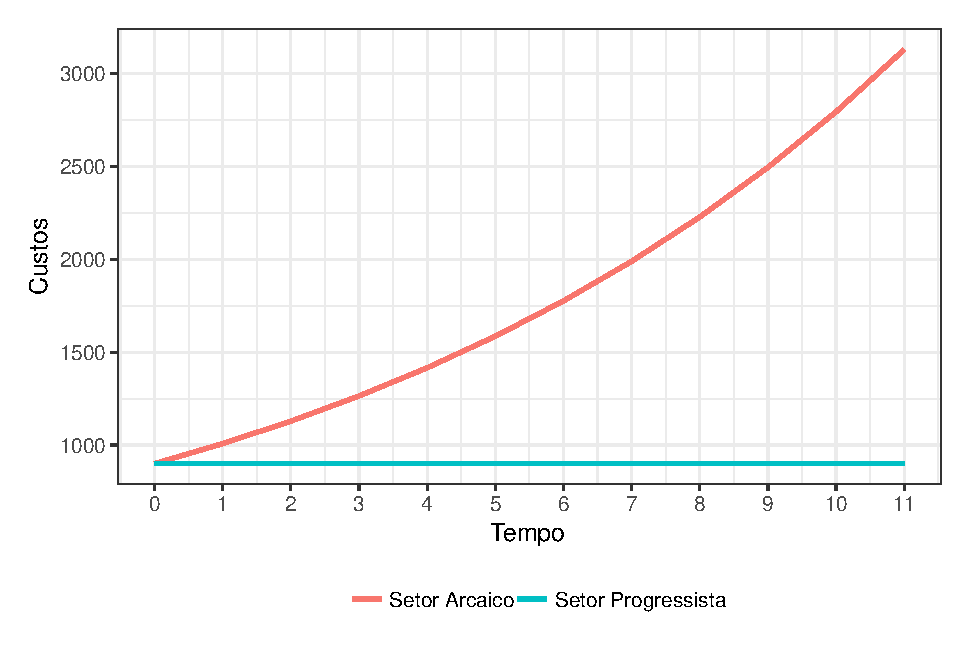
\includegraphics[scale=.8]{doenca_dos_custos.eps}
			\fonte{Elaboração do autor.}
		\end{figure}


		\item ``A demanda de espetáculos ao vivo é elástica; toda alta de preço redunda numa redução do público'' \cite[p. 56]{benhamou2007economia}. Sendo os preços proporcionais aos custos relativos nos dois setores, $P_1 = \alpha C_1$ e $P_2 = \beta C_2$, então
		$$\frac{P_1Y_1}{P_2Y_2} = \frac{\alpha C_1Y_1}{\beta C_2Y_2} = Cte$$ ou
		$$\frac{C_1Y_1}{C_2Y_2} = \frac{W(1+r)^t \cdot L_{1,t}}{W(1+r)^t \cdot L_{2,t}} = \frac{L_{1,t}}{L_{2,t}} = K_0$$ e
		$$\frac{Y_1}{Y_2} = \frac{aL_{1,t}}{bL_{2,t}(1+r)^t} = \frac{aK_0}{b(1+r)^t}$$

		``Quando \textit{t} aumenta, $\frac{Y_1}{Y_2}$ diminui, e quando $t \rightarrow \infty$, $\frac{Y_1}{Y_2} \rightarrow 0$'' \cite[p. 57]{benhamou2007economia}. Desse modo, a produção do setor arcaico (1) diminui fatalmente.
	\end{enumerate}

	De forma complementar à lei de Baumol, \citeonline{throsby1994production} desenvolve uma função da produção do espetáculo ao vivo a qual pode ser sintetizada da seguinte forma:

	O número de representações de uma determinada temporada deve ser fixado levando em conta a capacidade da sala \textit{v}. Sejam $L^s$ e $K^s$ o trabalho e o capital necessários para montar uma produção, sejam $L^r$ e $K^r$ o trabalho e o capital requeridos por cada representação da produção, o número de espectadores da iésima representação da jésima produção, $y_{ij}$, tal que $y_{ij} \leq v$, é dado por
	$$y_j = \sum_iy_{ij} = y_i(L^{s}_{j}, K^{s}_{j}, m_j, q_j) $$ onde
	o número de representações da jésima produção $$m_j = m_j(L^{r}_{j}, K^{r}_{j})$$ e $q_j$ resume as qualidades da jésima produção as quais, nesse contexto, podem ser medidas pela luxuosidade (\textit{lavishness}) da produção. Nesse caso, $q_j$ não é independente de $L^s$ e $K^s$. Espera-se que $$\frac{\partial y_j}{\partial m_j} > 0 \quad, \quad \frac{\partial^2y_j}{\partial m^{2}_{j}} < 0,$$ isto é, extender a temporada pode reduzir o número de espectadores na margem.

	Segundo \citeonline[p. 59]{benhamou2007economia} ``a conclusão do modelo [de Baumol] é a inelutabilidade do aumento dos déficits dos espetáculos ao vivo''. Esse modelo tem sido corroborado por várias pesquisas \cite[e.g.]{throsby1979economics,leroy1980economie,peacock1983inflation,baumol1984inflation,dias2011artes} e, para \citeonline[p. 54]{benhamou2007economia}, essa característica do setor é suficiente para justificar o aumento das subvenções públicas e da prática do mecenato mesmo tendo em vista que ``essa intervenção maciça, distribuída de forma muito desigual, não é suficiente para garantir ao setor um equilíbrio financeiro duradouro''. Para \apudonline[p. 320]{baumol1966performing}{luksetich2011orchestras}, ``se se concorda que a artes de performance conferem benefícios gerais à comunidade como um todo\ldots as artes são bens públicos cujos benefícios demonstravelmente excedem as receitas que se espera coletar na bilheteria\footnote{If one agrees that the performing arts confer general benefits on the community as a whole\ldots the arts are public goods whose benefits demonstrably exceed the receipts one can hope to collect at the box office.}''. O modelo, entretanto, possui inconsistências, algumas delas apontadas por \citeonline{benhamou2007economia}.

	A primeira consiste do pressuposto de que os salários do setor 1 são iguais aos do setor 2. Entretanto, desde a Segunda Guerra Mundial, os salários médios no setor do espetáculo ao vivo apresentaram uma tendência a crescerem menos do que no outro setor \apud{throsby1994production}{benhamou2007economia}. A segunda consiste do pressuposto altamente discutível de que a demanda é sensível ao preço. Maior parece ser o efeito da qualidade (percebida) do espetáculo sobre a demanda. De fato, \citeonline{throsby1994production} salienta que, por causa da dificuldade na medição da qualidade das performances, os efeitos dessa variável usualmente ficam restritos ao termo do erro nos modelos econométricos com a exceção de um estudo experimental conduzido pelo próprio \citeonline{throsby1983quality}. Nesse trabalho, o autor identificou algumas características da qualidade da performance no teatro como a qualidade da atuação, da produção, do roteiro e encontrou que a demanda é inelástica com relação ao preço dos ingressos mas \textit{altamente correlacionada com a qualidade esperada}. Este ponto parece central na investigação do mercado das orquestras e será desenvolvido oportunamente.

	Além disso, é possível reduzir os custos de uma produção de espetáculo ao vivo de várias formas, a saber, através da gravação e reprodução do espetáculo, através do uso, na música, de sons \textit{sampleados} ou eletrônicos ao invés da contratação de músicos, a utilização de um mesmo ator representando mais de um papel em uma montagem cênica ou a reutilização de cenários e figurinos (práticas comum em montagens modernas de ópera), dentre várias outras. Para \citeonline[p. 60]{benhamou2007economia} esses meios ``equivalem a substituir o déficit comercial por um `déficit artístico'. Mesmo assim, essas medidas não são suficientes para compensar a diferença de produtividade.

	A terceira inconsistência reside no fato de que a alta da produtividade nos setores progressistas acompanhada por um aumento de salário proporcional à melhora das qualificações provoca um crescimento da procura por espetáculos, o que \textit{per se} contribui com a solução das dificuldades criadas pela diferença de produtividade nos setores \apud{throsby1979economics}{benhamou2007economia}. O crescimento, para \apudonline{baumol1966performing}{benhamou2007economia} reside na presença de consumidores cada vez mais sagazes e exigentes e acaba por gerar custos marginais superiores às receitas. ``As companhias musicais ajudaram a construir a reputação de artistas cuja contratação se tornou inevitável. A consequência é um aumento exagerado dos cachês e dos custos'' \cite[p. 61]{benhamou2007economia}.

	Por mais que seja verdadeira esta última constatação sobre os custos gerados na contratação de artistas de renome, parece também uma grande ingenuidade acreditar que o aumento de salário acarreta um crescimento na procura por espetáculos ao vivo. Na verdade os estudos em sociologia econômica tem mostrado, como veremos, que o consumo artístico está ligado ao que Bourdieu (\citeyear{bourdieu2011forms,bourdieu2003amor,bourdieu2007distincao}) chama de ``capital cultural'' e à construção de uma identidade social.

	A quarta inconsistência é esta: A gravação dos espetáculos pode gerar receita. Embora as rendas de espetáculos gravados sejam pequenas conforme investigações no contexto americano \apud{heilbrun2001economics}{benhamou2007economia} parecem ser um recurso bastante explorado no setor Algumas orquestras brasileiras costumam disponibilizar as gravações de seus concertos e óperas como produto secundário da sua carta de produtos. Gravações de estúdio e ainda outros produtos (camisetas, acessórios, \textit{souvenirs}) compõem o financiamento dessas instituições. Oportunamente abordaremos esse ponto.

	\citeonline{throsby1994production}, após revisar vários estudos que testam a lei de Baumol conclui que

	\begin{citacao}
		Os impactos combinados dos ajustes de produção aumentaram a demanda e níveis crescentes de receita não esperada contrariaram qualquer tendência em direção a um aumento secular nos déficits entre companias de performance sugerindo que, embora a doença dos custos irá indubitavelmente continuar a presentear a artes performáticas com problemas difíceis, é improvável que chegue ao extremo\footnote{the combined impacts of production adjustments increased demand, and generally rising levels of unearned revenue have countered any tendency towards a secular rise in deficits among performance companies, suggesting that although the cost disease will doubtless continue to present the performing arts with difficult problems, it is unlikely to be terminal.}. \cite[p. 16]{throsby1994production}
	\end{citacao}

	Por fim, a análise de \citeonline{baumol1966performing} apontando a especificidade do setor contribuiu tanto para o desenvolvimento do programa de pesquisa que hoje conhecemos como economia da cultura quanto para o reconhecimento da necessidade de vinculação dos espetáculos ao vivo à esfera não-comercial subvencionada. Sigamos agora examinando como o mercado cultural brasileiro obtém seus recursos e o principal mecanismo de financiamento para que isso aconteça: as leis de incentivo à cultura.

	\section{Políticas Culturais no Brasil}

	Para \citeonline[p. 62]{benhamou2007economia}, ``na França, o espetáculo ao vivo vive essencialmente das subvenções públicas''. A realidade brasileira não parece ser diferente. No Brasil, a música de concerto, bem como as artes em geral, parecem obter a maior parte de seu financiamento através do Estado seja por investimento direto, seja por investimento indireto via isenção fiscal. No contexto brasileiro, a mais substantiva política pública na área da cultura reside na implementação de mecanismos de fomento à produção cultural mediante isenção fiscal os quais conhecemos como ``leis de incentivo à cultura''. Para \citeonline{sarkovas2005incentivo} a receita dos empreendimentos culturais \textit{per se} não dão conta de suprir as demandas do setor. Por isso se fazem necessárias outras três fontes de financiamento, a saber,

	\begin{citacao}
		\_o Estado, que tem a responsabilidade de fomentar a criação artística e intelectual, e a distribuição do conhecimento, bases do progresso humano;\\
		\_o investimento social privado, evolução histórica do mecenato, meio pelo qual cidadãos e instituições privadas tornam-se agentes do desenvolvimento da sociedade;\\
		\_o patrocínio empresarial, estratégia de construção de marcas e de relacionamento com seus públicos, feita por associação com ações de interesse público. \cite[p. 22]{sarkovas2005incentivo}
	\end{citacao}

	Para \citeonline{sarkovas2005incentivo}, essas três fontes foram interconectadas na criação de um sistema de financiamento por isenção fiscal que culminou em nossa conhecida Lei de Incentivo à Cultura. Em 2 de julho de 1986 era sancionada a ``Lei Sarney'', o primeiro mecanismo de isenção fiscal do país. Essa lei permitia que contribuintes abatessem dos impostos a pagar parte da quantia que decidiram investir em instituições culturais. A lei foi revogada sem motivo aparente em 1990 dando lugar a iniciativas semelhantes organizadas pelos governos municipais. No fim do mesmo ano foi promulgada em São Paulo a ``Lei Mendonça'' que permitia dedução do ISS\footnote{Imposto sobre serviços de qualquer natureza.} e do IPTU\footnote{Imposto sobre propriedade predial e territorial urbana.}. Outros municípios brasileiros acompanharam a medida e alguns estados criaram um modelo de isenção fiscal cujo abatimento se dava sobre o ICMS\footnote{Imposto sobre a circulação de mercadorias e serviços.}. Em dezembro de 1991 o sociólogo e então secretário da cultura Sérgio Paulo Rouanet instaura o ``Programa Nacional de Apoio à Cultura'' que ficou conhecido como Lei Rouanet. O programa instituía os mesmos mecanismos de isenção fiscal da antiga Lei Sarney e instituía ainda dois novos instrumentos, o FNC (Fundo Nacional de Cultura) e o FICART (Fundos de Investimento Cultural e Artístico). Segundo \citeonline{sarkovas2005incentivo}, nenhum dos dois mecanismos vingou. Para ele,

	\begin{citacao}
		O FICART tornou-se letra morta porque seus benefícios foram largamente superados pelos níveis de dedução fiscal obscenos que seriam depois adotados em outros mecanismos. E o FNC jamais foi operado pelas regras primárias de um fundo público: transparência de critérios, acessibilidade paritária e primazia do mérito público. Desde que foi criado, seus recursos são arbitrariamente distribuídos segundo predileções e interesses do Ministério da Cultura. \cite[p. 22-3]{sarkovas2005incentivo}
	\end{citacao}

	Em 1997 a medida provisória 1.589 introduziria a dedução de 100\% para as áreas de artes cênicas, livros de valor artístico, literário ou humanístico, música erudita ou instrumental, circulação de exposições de artes plásticas e doações de acervos para bibliotecas públicas e para museus. Em sua gestão, o ministro da cultura Gilberto Gil iniciou um processo de consulta pública em diversos estados denominado ``Cultura para Todos'' visando aprimorar a Lei Rouanet. Para \citeonline{sarkovas2005incentivo}, apesar das boas intenções, a medida foi realizada sem planejamento estratégico adequado e falhou em prover soluções para os problemas encontrados no modelo de financiamento. Esses problemas se relacionam sobretudo ao modo de seleção de projetos a serem financiados pela lei o qual reside na iniciativa privada. Nas palavras desse autor,

	\begin{citacao}
		O financiamento por dedução fiscal transfere e pulveriza, aleatoriamente, o dinheiro e a responsabilidade pública para as empresas e por	isso não é o instrumento adequado para produzir os efeitos que Gil alega desejar: ``desconcentração e democratização dos recursos; ampliação da responsabilidade do Estado e do público beneficiado; qualificação do processo de seleção dos projetos; facilitação e	apoio aos pequenos empreendedores; desburocratização e melhoria dos instrumentos de gestão”. Seria mais eficaz, e menos demagógico, estudar os modelos de financiamento público	direto que funcionam, no Brasil e no mundo,	dentro e fora da área cultural. \cite[p. 25]{sarkovas2005incentivo}
	\end{citacao}

	Isso acontece porque, apesar de o financiamento acontecer através de isenção fiscal, ou seja, com dinheiro público, são as empresas privadas que selecionam os projetos nos quais pretendem ``investir''. Para \citeonline[p. 27]{sarkovas2005incentivo} ``empresas patrocinam para ampliar sua credibilidade, estimular a identificação e melhorar o relacionamento com seus públicos de interesse; agregar atributos e valorizar suas marcas; demonstrar sua participação social''. Desse modo, projetos com grande mérito artístico, cultural ou pedagógico seriam suplantados por projetos que tenham maior apelo de mercado ou que se identifiquem mais com o público alvo da empresa patrocinadora. Para \citeonline[pos. 524]{weiss2009estatais}, um dos pontos fracos da Lei Rouanet consiste justamente da ``desproporção de apoio entre projetos grandiosos e de entretenimento -- e, portanto, de grande apelo de marketing -- e projetos locais, ligados à formação'' além do baixo retorno de captações. Os autores argumentam que mesmo sendo o principal motor da atividade cultural no país tendo movimentado em 2008 cerca de R\$ 1,4 bilhão, o mecanismo gera desequilíbrios, visto que ``as empresas habituaram-se a patrocinar com dinheiro público e os produtores culturais a contar com essa captação como única alternativa''\cite[pos. 475]{weiss2009estatais}.


	No Brasil, o Estado aparece como a grande instituição financiadora e mantenedora da arte, seja através de investimentos diretos, seja por investimentos indiretos. Em outros países, entretanto, encontramos cenários diversos. Alguns divergem completamente onde o financiamento da cultura é focado no mercado e as instituições culturais preferem não se submeter às regras impostas pelo Estado, outros assemelham-se ao caso brasileiro embora com uma porcentagem muitíssimo menor de financiamento público. \citeonline{van2006making} estudou as diversas formas de intervenção estatal nas artes no contexto europeu e avaliou as asserções comuns no discurso da área que sustentam a legitimidade/necessidade dessa intervenção conceituando as diversas linguagens artísticas como bens públicos ou não.


	Após as considerações sobre as especificidades dos produtos culturais e uma investigação preliminar sobre o modelo de financiamento da cultura vigente no Brasil apresentados acima, revisaremos agora a base teórica escolhida para análise e a metodologia.
	
	%Baumol's analysis pointing the specificities of the cultural sector contributed to both the development of the research program that we know today as economy of culture and the recognition of the necessity of binding live performances to the subsidized non-commercial sphere. However, this approach is a standard economic one which, for the purposes of this investigation, lacks some of the social elements that are important to understand the shaping of a market, namely, institutions, social control, cooperation and social coordination, etc. Therefore, we will now try to build a theoretical framework inside social theory and accounting for the findings we have seen so far. Let us start presenting each of the elements we are going to aggregate in our analysis framework, namely, (1), White's $W(y)$ model, (2), Fligstein's theory, (3), normative isomorphisms and (4) multilevel networks.



	\chapter{Arcabouço Teórico e Metodologia}

        \section{A sociologia neoestrutural}
	
	A chamada sociologia neoestrutural (também conhecida como Análise de Redes Sociais ou Sociometria) concebe o mundo social como estruturas interconectadas, redes, compostas por laços sociais \cite{denooy2011exploratory}. A Análise de Redes Sociais não constitui, como alguns argumentam, uma nova metodologia ou técnica de pesquisa (embora se aproprie de técnicas matemáticas e estatísticas complexas para suas análises) mas, antes, um novo paradigma, uma nova forma de olhar para o mundo e perceber seu \textit{modus operandi}.
	
	Dados de dois tipos interessam à sociologia neoestrutural. O primeiro deles é o que podemos chamar \textit{atributos}, ou características gerais de cada unidade na estrutura a ser investigada. Atributos podem estar relacionados a atitudes, opiniões, comportamentos ou características de indivíduos ou grupos específicos. Normalmente, quando a unidade individual da rede em questão são pessoas, observamos a idade, o sexo, cor da pele, renda, anos de escolaridade, etc. Se as unidades da rede são, por exemplo, organizações, é comum observarmos orçamento anual, quantidade de funcionários, valor de custo fixo, receitas, natureza do negócio na qual a organização está inserida, etc. O segundo tipo é o que chamamos de \textit{dados relacionais} e consistem de contatos, conexões, laços que conectam um indivíduo a outro \cite{scott2017social,wasserman1994social,lazega2014redes}. De acordo com \citeonline[p. 3]{scott2017social}, esse dado ``não pode ser reduzido a propriedades dos agentes individuais em si. Relações não são propriedades dos agentes, mas de sistemas de agentes\footnote{[Relational Data] (\dots) cannot be reduced to the properties of the individual agents themselves. Relations are not the properties of agents, but of systems of agents.}''. Para \citeonline{lazega2014redes}, o dado do tipo relacional é o grande diferencial da sociologia neoestrutural (embora não deem menos importância aos atributos). Para esses autores, uma relação social pode ser entendida como um canal para troca ou transferência de recursos ou como interação ativa com outros membros participantes do mesmo coletivo social. Ainda segundo os autores, o pesquisador observa um sistema de interdependências que emerge das relações entre membros de uma coletividade para, a partir de suas observações
	
	\begin{citacao}
		(\dots) reconstituir um \textit{sistema de interdependências}, descrever a influência desse sistema no comportamento dos membros e as variadas maneiras que empregam para gerir essas interdependências e as formas adquiridas pelos processos sociais decorrentes dessa gestão: aprendizagens, solidariedades, controles sociais, regulações, para citar apenas os mais genéricos. \cite[p. 5]{lazega2014redes}
	\end{citacao}

	
	
	A sociologia neoestrutural consiste, portanto, de um grande avanço no corpo teórico sociológico tradicional posto que abandona a velha dicotomia insolúvel entre agência e estrutura mas concebe o mundo como uma estrutura de indivíduos interdependentes onde tanto a ação individual quanto a força estrutural sobre o indivíduo emergem da própria estrutura e moldam-se uma à outra mutuamente \cite{white2008,higgins2018analise}.
	
	\subsection{Representação}
	
	Do ponto de vista técnico, as redes podem ser representadas de duas formas, utilizando matrizes e grafos. No caso das redes de 1 modo (redes construídas observando-se laços entre entidades da mesma natureza) a matriz é sempre quadrada de tamanho $m \times m$ onde cada linha e cada coluna corresponde a um ator da estrutura. Podemos, por exemplo, representar uma rede da seguinte maneira:
	
	\begin{equation}
	\label{example-matrix}
	M = \begin{pmatrix}
		0 & 1 & 1 & 1 & 1 \\
		1 & 0 & 0 & 0 & 0 \\
		1 & 0 & 0 & 0 & 0 \\
		1 & 0 & 0 & 0 & 0 \\
		1 & 0 & 0 & 0 & 0 \\
	\end{pmatrix}
	\end{equation}
	
	A matriz de adjacência \ref{example-matrix} representa uma rede binária, isto é, cada célula assume apenas a informação da existência ou não de um dado laço. No exemplo dado, o ator 2 possui um laço com o ator 1, o ator 3 possui laço com o ator 1, igualmente os atores 4 e 5. Normalmente, em redes de 1 modo, a diagonal da matriz é ignorada\footnote{Um valor igual a 1 numa célula diagonal indicaria que um ator possui uma relação com ele mesmo, o que chamado de \textit{looping}. Muito embora existam casos em que seja ontologicamente plausível que um ator possua uma relação consigo mesmo (voto, por exemplo), isso não é muito comum.}. A representação matricial é fundamental para a Análise de Redes Sociais pois é a partir dela que serão realizados os cálculos matemáticos dos escores e métricas típicos da abordagem. A mesma estrutura pode ser também representada a partir de um grafo (cf. Figura \ref{example-graph}).
	
	
	\begin{figure}[!ht]
		\centering
		\caption{Exemplo de grafo não direcionado}
		\label{example-graph}
		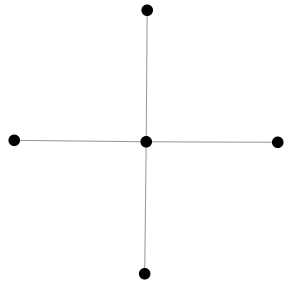
\includegraphics[scale=.4]{example-graph.png}
		\fonte{Elaboração do autor.}
	\end{figure}

	O grafo representado na Figura \ref{example-graph} é também um grafo não direcionado, ou seja, os laços nele observados não possuem direção inerente. Este é o caso, por exemplo, de redes de parentesco e matrimônio. Os grafos são compostos por pontos chamados \textit{vértices} ou \textit{nós} e conexões entre eles chamados de \textit{arestas} ou \textit{laços}. Existem também redes direcionadas, ou seja, cujos laços possuem direção inerente. Este é o caso, por exemplo, de redes de compra e venda, de trocas de recursos, de pedidos de conselho, etc. Além disso, podemos ter uma rede \textit{valorada} ou \textit{balanceada} quando os laços entre os vértices possuem pesos distintos. É possível, por exemplo, representar o volume de trocas econômicas entre empresas usando o valor do laço entre os vértices que as representam. Por outro lado, quando falamos de redes de amizade, por exemplo, o peso está associado ao conceito de \textit{força do laço} onde, usualmente, quanto mais tempo dois indivíduos passam juntos ou quanto maior for a carga emocional da relação, maior será o peso do laço\footnote{A esse respeito, consultar o trabalho seminal de \citeonline{granovetter1973strength}}.
	
	Uma rede direcionada e valorada poderia ser representada a partir da matriz \ref{weighted-matrix} e do grafo da Figura \ref{weighted-graph}.
	
	\begin{equation}
	\label{weighted-matrix}
	M = \begin{pmatrix}
	0 & 1 & 2 & 0 & 1 \\
	1 & 0 & 0 & 1 & 0 \\
	2 & 1 & 0 & 0 & 0 \\
	0 & 0 & 3 & 0 & 0 \\
	3 & 0 & 0 & 1 & 0 \\
	\end{pmatrix}
	\end{equation}
	
	
	\begin{figure}[!ht]
		\centering
		\caption{Exemplo de grafo direcionado e valorado}
		\label{weighted-graph}
		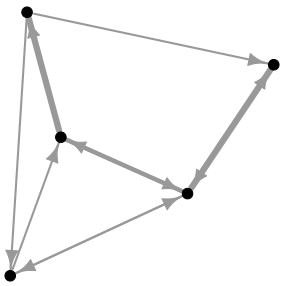
\includegraphics[scale=.4]{weighted-graph.png}
		\fonte{Elaboração do autor.}
	\end{figure}
	
	
	\subsection{Análise topológica da estrutra}
	
	As análises preliminares realizadas numa rede comumente abordam sua topologia. Trata-se de uma análise mais descritiva da estrutura. Isso não significa, entretanto, que a partir dela não possam ser feitas interpretações sociológicas profundas. Pelo contrário; é comum as primeiras análises trazerem excelentes esclarecimentos sobre a estrutura, até mesmo a análise visual da disposição dos vértices no plano\footnote{Aqui é pertinente comentar com o leitor que a disposição dos vértices no espaço não é algo trivial. Existem diversos algoritmos elaborados para isso hoje conhecidos na literatura e disponibilizados nos principais softwares de análise de redes sociais. Um \textit{layout} mal feito pode levar a \textit{insights} equivocados.} a qual, \textit{per se}, já é uma poderosa ferramenta analítica.
	
	A partir da matriz de adjacência podemos calcular a \textit{distância geodésica} entre dois vértices \textit{i} e \textit{j}, isto é, a distância mais curta em ``passos'' entre esses dois pontos. Quando a distância geodésica é pequena, podemos considerar que \textit{i} e \textit{j} estão próximos; quando é grande, podemos considerar que eles estão distantes. Do mesmo modo, o \textit{diâmetro} mostra a maior distância geodésica entre dois pontos observada na estrutura. Dizemos que um grafo é \textit{conectado} quando há um caminho ligando todos os seus vértices.
	
	A \textit{densidade} da rede pode ser calculada tomando-se o número de laços observados sobre o número de laços possíveis na estrutura. O cálculo pode ser definido por $$\delta = \frac{L}{g(g-1)}$$ onde $g$ é o número de vértices e $L$ o número de laços observados. Esta medida é um indicador de base da estrutura da rede e tende a diminuir quando o tamanho da rede aumenta \cite{lazega2014redes}. Se a rede sob investigação for valorada, a métrica pode representar a força média dos laços. No geral, quanto mais denso for um grafo, mais conectado ele é.
	
	\subsubsection{As medidas de centralidade}
	
	Uma das medidas mais importantes na Análise de Redes Sociais é o escore de \textit{centralidade} o qual indica o posicionamento de um vértice em relação à estrutura. A partir dela, podemos identificar os atores mais ``importantes'' do sistema de acordo com alguns critérios. As medidas de centralidade estão normalmente associadas a duas condições sociais, a saber, o \textit{prestígio} e a \textit{atividade}. No caso das redes direcionadas, podemos dizer que um indivíduo possui alto prestígio quando recebe muitos laços; de forma análoga, podemos dizer que um indivíduo é muito ativo na rede quando envia muitos laços. Nos casos das redes não direcionadas não é possível fazer essa distinção visto que o laço não possui direção intrínseca. Falamos, nesses casos, de centralidade de uma forma mais geral, como importância \cite{lazega2014redes}.
	
	As três medidas de centralidade mais comuns na literatura são a centralidade de grau (\textit{degree centrality}), a centralidade de intermediação (\textit{betweeness centrality}) e a centralidade de proximidade (\textit{closeness centrality}).
	
	A centralidade de grau de um nó é igual à força dos laços que ele possui. Nesse aspecto, quanto mais conectado com outros um ator tiver e quanto mais fortes forem seus laços, mais central ele será. 
	
	``A centralidade de proximidade de um ator é medida pelo número mínimo de passos que ele deve fazer para entrar em contato com os outros atores no sistema'' \cite[p. 43]{lazega2014redes}. Nesse aspecto, quanto mais próximo dos demais um ator estiver, mais central será pois poderá interagir com maior facilidade. A centralidade de proximidade é definida por $$C_{pro} = \frac{1}{\sum_{j=i}^{g} d_{ij}}$$ onde $d_{ij}$ é a distância geodésica entre os atores \textit{i} e \textit{j}. ``A distância total entre o ator \textit{i} e todos os outros é $\sum_{j=i}^{g} d_{ij}$ onde a soma se efetua para todos os $j \neq i$'' \cite[p. 44]{lazega2014redes}. Trata-se do inverso da soma das distâncias entre um ator \textit{i} e os demais na estrutura. Seu valor máximo é $1/(g-1)$
	
	A centralidade de intermediação se baseia na ideia de que dois indivíduos podem ser intermediados por um terceiro com os quais ambos possuem laço. Essa posição central é privilegiada pois pode interromper o fluxo de recursos ou informação. Quanto mais um ator se encontra ``no meio'', mais central ele é nesse critério. A centralidade de intermediação é definida por $$C_{inter} = \frac{\sum_{j<k} g_{jk} (i)}{g_{jk}}$$ para $i \neq j, k$. Este índice representa a proporção das distâncias geodésicas entre \textit{j} e \textit{k} que passam por \textit{i}. $g_{jk}$ representa o conjunto das geodésicas entre \textit{j} e \textit{k} e $g_{jk}(i)$ é um caminho entre \textit{j} e \textit{k} passando por \textit{i}. Essa medida pode chegar ao máximo de $(g-1)(g-2)/2$ e encontrará seu valor máximo quando um ator se encontrar em todas as geodésicas. 
	
	\subsubsection{Os buracos estruturais}

	Para além das medidas de centralidade mencionadas acima, o sociólogo Ronald Burt (\citeyear{burt1982toward,burt1992structural,burt2005brokerage}) desenvolveu uma medida de autonomia e restrição estruturais. A medida chamada \textit{constraint} consiste de um escore que leva em conta não apenas o posicionamento do indivíduo na estrutura mas também o perfil relacional de seus vizinhos. 
	
	Baseado na \textit{densidade proporcional} da sub-rede de cada ator, Burt mede a restrição que \textit{i} exerce sobre \textit{j} através das interações diretas entre esses dois vértices e da força e quantidade de laços que \textit{j} possui com outros alters de \textit{i}. A restrição ocorre porque o ator não pode substituir seu álter por outro. ``Logo, a autonomia significa, antes de tudo, a capacidade de substituir uma relação por outra; de ter uma alternativa relacional'' \cite[p. 71]{lazega2014redes}. Quanto maior for a restrição global que uma rede impõe sobre um ator, mais ``constrangido'' ele será; quanto menor for a restrição global da rede sobre o ator, maior liberdade de atuação na estrutura ele possui e ``mais se encontra em posição de beneficiar de oportunidades muito ricas em ganhos de toda natureza (sobretudo em informação e controle), tornando-se um intermediário indispensável a outros atores'' (\Ibidem{lazega2014redes}). Esta é a principal medida entre os analistas de redes para investigar o \textit{capital social}. Sua lógica obedece a descrição abaixo de \citeonline{lazega2014redes}:
	
	\begin{citacao}
		Quanto mais alters ``não redundantes'' eu tiver em minha rede, mais minhas relações serão únicas, mais chances tenho de ser paralisado pela estrutura (\textit{aggregate constraint}). Quanto mais estiver vinculado a atores não vinculados entre si, mais serei intermediário entre posições não centralizadas, mais ``buracos estruturais'' haverá (ausência de relações entre posições) na rede e mais poderei beneficiar das oportunidades oferecidas por essas ausências de relações. \cite[p. 71-2]{lazega2014redes}
	\end{citacao}

	A densidade proporcional pode ser definida por 
	
	\begin{equation}
	p_{ij} = \frac{\sum_j \sum_q \delta_{ij}}{N (N - 1)}, \quad j \neq q
	\end{equation}
	
	onde $\delta_{ij}$ é igual a 1 se $z_{ij}$ não for igual a zero. A partir dela, podemos calcular o \textit{constraint}, o nível de restrição que um alter \textit{j} impõe sobre \textit{i} usando
	
	\begin{equation}
	c_{ij} = \left(p_{ij} + \left[\sum_q p_{iq} p_{qj} \right]\right)^2 O_j, \quad q \neq i,j
	\end{equation}
	
	onde $p_{ij}$ representa a densidade proporcional e $O_j$ é uma medida da organização dos atores que pertencem ao mesmo subconjunto de \textit{j}. O \textit{constraint} agregado é, portanto, a soma de todas as restrições a \textit{i} provenientes das relações que ele tem com cada um de seus alters: $c_i = \sum_j c_{ij}$. É conhecido na literatura, entretanto, que este índice perde sua qualidade quando a rede investigada é muito grande.
	
	
	\subsubsection{Equivalência estrutural}
	
	Para além da descrição do posicionamento relacional e do grau de autonomia/liberdade que um ator possui numa rede, a Análise de Redes Sociais está também interessada na investigação de \textit{papeis sociais}. Segundo \citeonline{scott2017social}, essa análise faz sentido quando na estrutura é possível observar pessoas ocupando papeis institucionalizados, papeis que sejam culturalmente bem definidos. A partir da identificação de atores que possuem o mesmo perfil relacional, ou seja, se relacionam de forma similar com alters similares, podemos afirmar que eles são \textit{estruturalmente equivalentes}, ou seja, cumprem a mesma função na rede e são portanto, intercambiáveis.
	
	\citeonline{lazega2014redes} argumentam que a equivalência estrutural é uma propriedade matemática matricial praticamente impossível de ser observada na vida social pois dois atores nunca possuem um perfil relacional idêntico. Entretanto, a partir das semelhanças do perfil relacional é possível constituir posições bem delimitadas. Para esses autores, o conceito de equivalência estrutural é o que distingue a abordagem neoestrutural da sociometria clássica.
	
	A equivalência estrutural pode ser medida de diversas maneiras embora duas delas sejam privilegiadas na literatura. Ambas são métodos de cálculo de \textit{blockmodels}, modelos de blocos categóricos. O blockmodel pode utilizar a correlação como medida de equivalência correlacionando tanto linhas (laços enviados) quanto colunas (laços recebidos) \cite{lazega2014redes}. O principal algoritmo utilizado para calcular o blockmodel a partir de correlações é o \textit{CONCOR} (\textit{Convergence of Iterated Correlations}) desenvoldido por \citeonline{white1976social}. Nesse algoritmo são calculadas as correlações para cada par de atores e elaborada uma nova matriz quadrada com os valores das correlações. A partir daí, para cada par, são calculadas novas correlações sobre as correlações calculadas anteriormente. Esse processo se repete até que a matriz final fique com valores iguais a $+1$ ou $-1$, ou seja, o padrão iterativo de correlações converge numa matriz com um critério forte de segmentação que pode ser dividida em dois clusters. Cada um dos clusters pode ser dividido novamente pelo mesmo critério até que o pesquisador decida pelo número desejado de clusters obtidos \cite{scott2017social}.
	
	Seja $x_{ik}$ o valor do laço entre os atores \textit{i} e \textit{k}. A correlação como critério de medida para a equivalência estrutural pode ser definida por
	
	\begin{equation}
	r_{ij} = \frac{\sum(x_{ki} - \bar{x}_{oi})(x_{kj} - \bar{x}_{oj}) + \sum(x_{ik} - \bar{x}_{io})(x_{jk} - \bar{x}_{jo})}{\sqrt{ \sum(x_{ki} - \bar{x}_{oi})^2 + \sum(x_{ik} - \bar{x}_{io})^2} \sqrt{\sum(x_{kj} - \bar{x}_{oj})^2 + \sum(x_{jk} - \bar{x}_{jo})^2}}
	\end{equation}
	
	onde $\bar{x}_{io}$ denota a média dos valores na linha \textit{i} e $\bar{x}_{oi}$ denota a média dos valores na coluna \textit{i} e todas as somas são sobre \textit{k}, $i \neq k$, $j \neq k$ \cite{wasserman1994social}.
	
	Por outro lado, Burt (\citeyear{burt1976positions,burt1982toward}) propôs medir a equivalência estrutural como a distância Euclidiana entre os laços recebidos e enviados por \textit{i} e \textit{j}. Para esses atores, a distância entre as linhas \textit{i} e \textit{j} e colunas \textit{i} e \textit{j} da matriz de adjacências pode ser definida por
	
	\begin{equation}
	d_{ij} = \sqrt{\sum_{k=1}^{g} [(x_{ik} - x_{jk})^2 + (x_{ki} - x_{kj})^2 ] }
	\end{equation}
	
	para $i \neq k$, $j \neq k$ \cite{wasserman1994social}. 
	
	
	O blockmodel retorna uma nova matriz com os atores agrupados em \textit{posições} estruturalmente equivalentes. A Figura \ref{example-socio-blocked-matrix} mostra, à esquerda, uma matriz de adjacência conforme observada e, à direita, sua permutação para privilegiar a visualização dos grupos após o blockmodel.
	
	
	\begin{figure}[!ht]
		\centering
		\caption{Matriz de adjacência observada e reorganizada após blockmodel}
		\label{example-socio-blocked-matrix}
		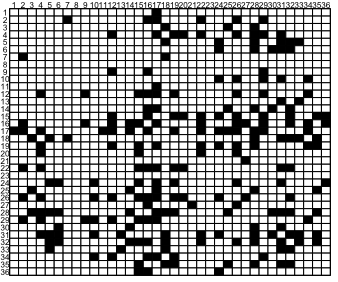
\includegraphics[scale=.6]{example_sociomatrix.png}
		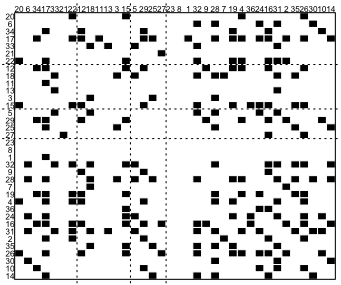
\includegraphics[scale=.6]{example_blockedmatrix.png}
		%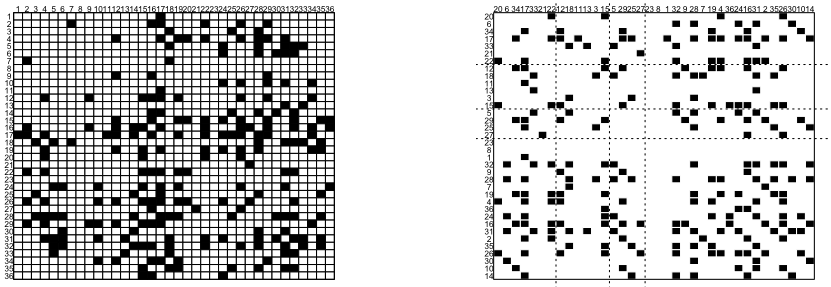
\includegraphics[scale=.5]{example_socio_and_blockedmatrix.png}
		\fonte{Elaborado pelo autor usando o pacote \textit{sna} \cite{snapackage}}
	\end{figure}
	
	A nova matriz pode ser representada agora através das densidades entre grupos e dentro dos grupos conforme a matriz da Tabela \ref{matriz-densidade}.
	
	% latex table generated in R 3.5.1 by xtable 1.8-3 package
	% Sat Dec 29 12:44:07 2018
	\begin{table}[ht]
		\ibgetab{
		\centering
		\caption{Matriz de densidades}
		\label{matriz-densidade}
	}
		{\begin{tabular}{rrrrr}
			\hline
			& Bloco 1 & Bloco 2 & Bloco 3 & Bloco 4 \\ 
			\hline
			Bloco 1 & 0.20 & 0.17 & 0.18 & 0.20 \\ 
			Bloco 2 & 0.17 & 0.13 & 0.17 & 0.17 \\ 
			Bloco 3 & 0.18 & 0.17 & 0.00 & 0.18 \\ 
			Bloco 4 & 0.20 & 0.17 & 0.18 & 0.14 \\ 
			\hline
		\end{tabular}
	}
	{\fonte{Elaborado pelo autor.} }
	\end{table}


	% enviar para estratégia metodológica	
	% Para investigar os nichos de qualidade dos mercado, identificaremos equivalência estrutural entre atores usando Blockmodels como proposto por \citeonline{lazega2009theorie}. Isso nos permitirá reduzir a complexidade das redes identificando nichos de mercado. 
	
	%On accounting for the multilevel networks, we will adopt the analysis strategy described by \citeonline{brailly2016market}. We will use ERGM's to test our hypotheses regarding relations within each level and 2-mode to 1-mode transformations to investigate the affiliations between levels. We will briefly explain the rationale of the models.
	
	
	Na análise empreendida neste trabalho utilizaremos uma versão estocástica frequentista do modelo elaborada por \citeonline{daudin2008mixture} e uma versão estocástica bayesiana elaborada por \citeonline{latouche2012variational}\footnote{Maiores esclarecimentos sobre essas variações dos blockmodels serão apresentadas oportunamente.}
	
	%In this research we will use a stochastic frequentist version of the model elaborated by \citeonline{daudin2008mixture} and a stochastic bayesian version elaborated by \citeonline{latouche2012variational}.
	
	
	
	\subsection{Modelos probabilísticos com dados relacionais}
	
	Uma análise sociológica com dados relacionais profunda e informativa depende de um uso consciente das métricas características do paradigma mas também de técnicas probabilísticas que permitam modelar os processos sociais a partir dos atributos dos atores e das configurações internas da estrutura sob investigação. É fundamental entender o processo de escolhas sociométricas dos atores para explicar comportamentos, crenças, escolhas relacionais e normativas, etc \cite{lazega2014redes}.
	
	Contudo, o dado relacional apresenta problemas específicos quando utilizado em modelos estatísticos. Nos casos em que variáveis relacionais são utilizadas como variáveis independentes (escores de centralidade, autonomia, etc.), ou seja, variáveis que explicam algum fenômeno social, há grandes chances de multicolinearidade pois as diversas métricas relacionais tendem a ser altamente correlacionadas entre si.
	
	Em outros casos, os dados relacionais são variáveis dependentes, ou seja, aquilo que se busca explicar. ``É o caso quando se busca explicar porque alguns atores tem mais facilmente acesso a um maior número de recursos, ou identificar os critérios que utilizam para escolher ou selecionar suas relações'' \cite[p. 76]{lazega2014redes}. Investigamos aqui o impacto que a própria estrutura de interdependências bem como os atributos do indivíduo (como escolaridade, renda, cor da pele, status, gênero, etc.) tem nas escolhas relacionais observadas. O dado relacional, contudo, fere um pressuposto básico da análise estatística convencional, qual seja, a \textit{independência das observações} \cite{gujarati2011econometria}. É necessário, portanto, um tipo de modelo estatístico que leve em conta as interdependências das observações.
	
	A partir da década de 1980 surgiu um conjunto de modelos desde o primeiro batizado modelo $p_1$ de \citeonline{holland1981exponential} até os recentes ERGM's (\textit{Exponential Random Graph Models}) que dividem a rede em subestruturas de díades, tríades e configurações de ordem superior (\textit{high order}) e estimam parâmetros para uma melhor compreensão do sistema tanto em seu aspecto individual quanto coletivo.
	
	\begin{citacao}
		Essa ideia se baseia no postulado de \citeonline{holland1981exponential} segundo o qual é possível compreender os mecanismos e processos em jogo em uma rede, se nos interessarmos unicamente pelas estruturas locais, na medida em que estas últimas são dependentes entre si. Porém, como demonstrado por \citeonline{besag1974spatial} e \citeonline{frank1986markov}, a consideração da dependência de estrutura permite reduzir o conjunto dos grafos possíveis condicionalmente às estruturas -- ou configurações -- especificadas. \cite[p. 78]{lazega2014redes}
	\end{citacao}
	
	
	
	\subsubsection{Noções básicas do ERGM}
	
	Os ERGM's, \cite{robins2007introduction,lusher2013exponential,lazega2014redes,brailly2017explorer}, são modelos estatísticos desenvolvidos especificamente para dados relacionais. Uma estrutura de relações postula interdependência entre as identidades que a compõem. Isso fere um dos pressupostos da modelagem estatística convencional, qual seja, a independência das informações. ``O fato de que eu escolho Pedro como amigo não é necessariamente independente do fato de que eu também escolho Paulo porque eles também podem ser amigos entre si \cite[p. 76]{lazega2014redes}.
	
	%ERGM's are statistical models developed specifically to deal with relational data \cite{robins2007introduction,lusher2013exponential}. A relations structure postulates interdependence between identities. This goes against one of the assumptions of conventional statistical modeling, the independence of information. ``The fact that I choose Peter as my friend is not necessarily independent of the fact that I also choose Paul because they can be friends with each other'' \cite[p. 76]{lazega2014redes}.
	
	A segmentação da estrutura em rede em tríades mencionada acima ocorre a partir da classificação \textit{MAN} (sigla para \textit{Mutual, Asymmetric, Null}). Esse esquema classifica as díades dentro das tríades observadas com 3 algarismo, o primeiro indicando o número de laços mútuos, o segundo indicando o número de laços assimétricos e o terceiro indicando o número de laços nulos ou inexistentes. O esquema também faz uso das letras U (\textit{up}), D (\textit{down}), T (\textit{transitive}) e C (\textit{cyclic}) para diferenciar a direção dos laços quando necessário. Um exemplo das configurações possíveis está apresentado na Figura \ref{triades-man}.
	
	
	\begin{figure}[!ht]
		\centering
		\caption{Tipos de isomorfismos de tríades com a nomemclatura \textit{MAN}}
		\label{triades-man}
		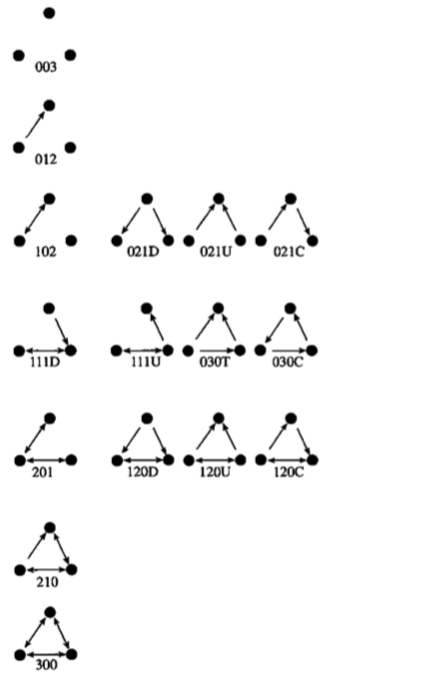
\includegraphics[scale=.6]{triades.png}
		\fonte{\cite[p. 566]{wasserman1994social}}
	\end{figure}
	
	Cada uma das configurações do esquema \textit{MAN} pode indicar um processo social. Para citar alguns exemplos, a configuração 102 indica reciprocidade, 021D indica atividade 021U indica prestígio, 030T indica transitividade, 030C indica relações cíclicas (a solidariedade no sentido da troca generalizada de Lévi-Strauss).
	
	Para além das configurações endógenas da própria rede, os últimos avanços do modelo incluem ainda os atributos dos indivíduos e outras relações também mensuradas entre eles. Utilizando os atributos é possível investigar se a construção de laços é moldada por algum deles (e.g., homofilia). Utilizando outros laços mensurados é possível testar o efeito de de redes covariáveis, ou seja, em que medida esses outros laços condicionam a formação da rede em investigação. Por exemplo, \citeonline{crepalde2017social} investiga os laços de produção acadêmica conjunta e testa se a coautoria é moldada, no caso dos atributos, por participação nos mesmos grupos de pesquisa, por gênero, cor, renda ou produtividade acadêmica ou, no caso das redes covariáveis, se laços de pedidos de revisão, prestígio metodológico, prestígio teórico, amizade ou indicação profissional moldam a construção de laços de coautoria.
	
	
	
	Os ERGM's podem ser definidos por
	
	
	\begin{equation}
	Pr(Y=y) \quad = \quad \left(\frac{1}{k}\right) exp \left\{ \sum_{A} \eta_A g_A (\textbf{y}) \right\}
	\end{equation}
	
	onde $Y$ é o grafo teórico estimado, $y$ é o grafo observado, $\sum_{A}$ é a soma de todas as configurações \textit{A}, $\eta_A$ é o parâmetro estimado correspondente à configuração \textit{A}, $g_A(\textbf{y})$ é a estatística da rede correspondente à configuração \textit{A} no grafo \textbf{y} e \textit{k} é uma constante que assegura uma distribuição de probabilidade adequada\cite{robins2007introduction}. 
	
	%Esta família de modelos nos permite estimar o efeito de cada configuração endógena na emergência da própria rede. Dito de outra maneira, visto que cada configuração endógena pode ser associada a um processo social, este modelo nos permite \textit{explicar a rede como uma variável dependente}, explicar quais processos são importantes e quais são secundários para entender a estrutura social em investigação.
	
	%where Y is the theoretical estimated graph, y is the observed graph, $\sum_{A}$ is the sum of all configurations \textit{A},  $\eta_A$ is the estimated parameter corresponding to configuration \textit{A}, $g_A(\textbf{y})$ is the network statistic corresponding to configuration \textit{A} of graph \textbf{y} and \textit{k} is a constant that ensures an adequate probabilities distribution \cite{robins2007introduction}. This model allows us to estimate the effect of each endogenous configuration of the network on the emergence of the network itself. Put another way, since every endogenous configuration can be associated with a social process, the model allows us to \textit{explain the network as a dependent variable}, to explain which processes are important and which are not important to understand the social structure under investigation. In our case, this procedure will be conducted for both levels of the network, that is, we will model both social processes modeling the inter-individual structure and the inter-organizational structure.
	
	
	
	

	%Para entender o mercado da música de concerto, é necessário um arcabouço teórico que o dê sentido e, ao mesmo tempo, conduza o olhar do pesquisador. No processo de pesquisa, foi possível identificar elementos de diversos \textit{frameworks} teóricos que lançam luz sobre o nosso objeto de estudo. Neste capítulo, nosso esforço se dará numa tentativa de articulação desses elementos de modo a obtermos um arcabouço teórico para análise de nosso objeto. Apresentaremos quatro elementos teóricos que lidam com a emergência dos mercados, a saber, o modelo relacional de Harrison White, o modelo de Fligstein, o conceito de \textit{coopetition} e o conceito de isomorfismos organizacionais.










        \subsubsection{Network Autocorrelation Models}

        Para além das situações em que desejamos explicar a própria rede como uma variável resposta, há alguns casos em que estaríamos interessados em explicar um atributo específico dos atores envolvidos. Nesses casos, uma solução interessante é provida pelo \textit{Network Autocorrelation Model}, ou NAM. O NAM foi proposto de duas maneiras; a primeira, como um modelo de autocorrelação a partir dos laços observados entre os atores da rede\footnote{Segundo \citeonline[p. 22]{leenders2002modeling}, ``Autocorrelation of either a variable (or error term) is the situation where the observations of variables (or error terms) for different actors are not independent over time, through space, or across a network''.}; a segunda como uma variação dos ERGM e chamado de \textit{Autologistic Actor Attribute Model} \cite{kashima2013acquisition,daraganova2013autologistic,daraganova_pattison_2013};
	A intuição básica desse modelo consiste da estimação de atributos dos atores como variáveis dependentes da estrutura relacional do ator e de outras covariáveis exógenas. Dito de outra forma ao invés de modelar a estrutura, este modelo estima um atributo específico dos atores. Nesse caso, ele difere dos métodos estatísticos convencionais como a regressão linear ou a regressão logística pois leva em conta a dependência das observações de modo que os atributos dos atores são dependentes uns dos outros por meio da relação diádica, isto é, se eles compartilham um laço.
	
	O \textit{Network Autocorrelation Model} pode ser definido por
	
	\begin{equation}\label{NAM}
	y = \rho W_y + X \beta + \epsilon, \quad \epsilon \sim \mathcal{N}(0, \sigma^2 1)
	\end{equation}
	
	onde \textit{y} representa o atributo estimado, $\rho W_y$ representa a matriz de adjacência da rede em questão (necessariamente uma matriz $m \times m$), $\beta$ representa o vetor de estimadores para as covariáveis da matriz $X$ e $\epsilon$, o erro do modelo.


        % Escrever aqui um conectivo conectivo conectivo


        Até aqui, buscamos apresentar uma visão geral do paradigma relacional o qual norteia toda a nossa investigação. A seguir, apresentamos o principal modelo teórico adotado neste trabalho, a saber, a teoria dos mercados de White.



        
	\section{Markets from Networks}

	Para Harrison \citeonline{white2002markets}, os mercados não são dados mas são estruturas sociais que emergem de interações complexas de seus componentes. Essas interações podem acontecer tanto de forma competitiva quanto, argumentamos, de forma cooperativa visando estabilização do mercado e redução do que o professor White chama de ``incerteza knightiana\footnote{Em referência ao economista americano Frank H. Knight. Para Knight, a incerteza se diferenciava do risco de que este representava uma probabilidade mensurável enquanto aquele relacionava-se a situações de diversos valores indeterminados e não quantificáveis, ou seja, uma situação de probabilidade numericamente imensurável \cite{andrade2011construccao}.}''.
        
	Sua teoria visa explicar ``como as firmas minimizam incertezas formando um mercado como uma coleção de nichos baseada em sinais observados em seus engajamentos\footnote{(...) how firms minimize uncertanty by forming a market as a collection of niches based on signals observed in their commitments.}'' \cite[p. xiii]{white2002markets}. Em que consiste, portanto, um mercado de produção? A resposta para essa pergunta perpassa duas dimensões. A primeira, já comentada no parágrafo acima, remonta à natureza interdependente de sua estrutura, ou seja, uma emergência a partir das dependências de seus próprios fluxos. A segunda remonta ao seu mecanismo de operação o qual consiste dos engajamentos das diversas firmas em fluxos de produtos nos quais a procura do comprador agregado foi incorporada. Para esse autor ``Os fluxos resultantes de bens ou serviços diferenciados do mercado se dividem entre diversos compradores como opções igualmente boas: \textbf{a disciplina do mercado está centrada na qualidade do produto}\footnote{Resulting streams of differentiated goods or services from the market get split among diverse buyers as equally good options: The market discipline centers on product quality.}'' \cite[p. 1, grifo meu]{white2002markets}. Este ponto é central na caracterização de nosso objeto de estudo. O que seriam, entretanto, disciplinas de mercado?

	\citeonline[p. 63]{white2008} indica que ``disciplinas oferecem regras dos jogos que produzem coordenação em tarefas em um mundo que, do contrário, seria caótico\footnote{Disciplines offer rules of the games that yield coordination in tasks in an otherwise messy world.}''. As disciplinas permitem ações conjuntas dando ordem aos laços traçados entre identidades em rede. Cada disciplina possui um tipo de processo que agrega a ação conjunta. Elas possuem ainda um ordenamento de valor específico pelo qual a estrutura se organiza hierarquicamente (por isso, podemos entender as disciplinas também como um sistema local de status). Dentre os tipos ideais de disciplinas elencadas pelo autor, aquela que se aplica aos mercados é chamada de \textit{interface}. Seu processo típico é o \textit{engajamento} que gera fluxos produtivos. O valor distintivo típico desse tipo de disciplina é a \textit{qualidade}.

	No caso dos mercados de produção, as firmas engajam fluxos de produtos direcionados ao comprador agregado que são percebidos na interface do mercado como igualmente bons. O distintivo social, o ordenador de valor nessa estrutura, é a qualidade.

	Como se articulam os mercados? Para \citeonline{white2002markets}, algumas distinções básicas precisam ser feitas para entendermos sua estrutura. A primeira delas concerne a distinção entre \textit{downstream} e \textit{upstream}\footnote{Pela grande dificuldade em traduzir esses termos, optamos por mantê-los conforme o idioma original. Uma tentativa de tradução pouco elegante poderia ser feita como ``fluxos para baixo'' e ``fluxos para cima''.}, ou seja, os fluxos de produtos engajados pelo produtor em direção ao comprador agregado e a demanda desse comprador agregado o qual é incorporada nos produtos. Essa distinção gera uma segunda distinção concernente a três possíveis papeis para as firmas num mercado, a saber, fornecedor, produtor e comprador. Cada mercado possui uma orientação \textit{upstream} ou \textit{downstream}. Segundo o autor, ``os produtores não estão imbricados em um mercado, como o sociólogo Mark \citeonline{granovetter2007acao} argumentaria; eles de fato constituem a interface do mercado como um set de suas percepções e escolhas\footnote{Producers are not just embedded in a market, as the sociologist Mark Granovetter (1985) [na citação original] would argue; they actually constitute the market's interface in, and as the set of, their perceptions and choices.}'' \cite[p. 8]{white2002markets}. A constituição da interface do mercado se dá em direcionamento à origem percebida de risco. Nesse ponto, para White, reside a fraqueza da teoria econômica ortodoxa.

	Ora, a teoria econômica ortodoxa oferece várias tentativas de modelagem de mercados empíricos/realísticos e, para isso, ancora-se em várias asserções provenientes do senso comum. Muito embora esse corpo de conhecimento possua modelos econométricos sofisticados, ele reside muito próximo do senso comum. Entretanto, ao abordar fluxos de produtos em rede num ambiente realístico, a teoria econômica ortodoxa abandona seus modelos, sejam eles realísticos ou de senso comum, e se atém à ficção da competição perfeita. Para \citeonline[p. 9]{white2002markets} ``um enorme custo dessa ortodoxia tem sido a infiltração desapercebida de noções de competição pura na pesquisa de economistas práticos\footnote{One great cost of this orthodoxy has been the unacknowledged infiltration of notions of pure competition into practical economists' research.}''. Do mesmo modo, a sociologia também tem relutado em incorporar os achados da teoria econômica em tentativas de construir críticas mais gerais à influência econômica nos processos sociais a partir das pesquisas de mercados específicos.

	Como, então, podemos entender a estabilização de uma interface de mercado? Que propriedades dela podem sucumbir à ``incerteza knightiana'' que atua contra seus membros?

	\subsection{Estabilizando a ``incerteza knightiana''}

	Transações num mercado tem mais a ver com interações repetitivas do que com momentos únicos. Desse modo, o volume de fluxos de produtos em um mercado pode funcionar como um sinalizador para os produtores sobre os engajamentos. Nas palavras de White:

	\begin{citacao}
		Cada um [produtor] pode se orientar em direção a um nicho pelo tamanho que é apropriado à avaliação do mercado de sua própria qualidade comparada à de seus companheiros que também se orientarão aos nichos: o mercado como uma construção social conjunta\footnote{Each can orient to a niche by the size that is appropriate to the market's assessment of its quality compared to that of its fellows, who also are orienting to niches: the market as a joint social construction.}. \cite[p. 10]{white2002markets}
	\end{citacao}

	Atrelada à interface do mercado está a noção de qualidade que, embora seja comumente tomada por uma característica inerente aos produtos, emerge das interações entre julgamentos tanto de produtores quanto de compradores. Desse modo,

	\begin{citacao}
		É uma noção dual de qualidade diferencial referente tanto a produto como a produtor que se torna estabelecida como o centro em volta do qual um conjunto de solos sólidos\footnote{\citeonline{white2008} caracteriza os \textit{footings} ou solos sólidos como definições compartilhadas da vida social sobre a qual os indivíduos orientam sua ação e sua interpretação da ação do outro.} [\textit{footings}] para produtores pode se reproduzir como solos sólidos em um perfil de mercado conjunto. Os dois lados, compradores e produtores, exercem pressões concorrentes no formato desse perfil, pressões que são correlacionadas com suas respectivas discriminações de qualidade\footnote{(\dots) it is dual notions of differential quality, referent both to product and to producer, that become established as the core around which a set of market footings for producers can reproduce itself as footings in a joint market profile. The two sides, buyers and producers, exert contending pressures on the shape of this profile, pressures that correlate with their respective discriminations of quality.}. \cite[p. 10]{white2002markets}
	\end{citacao}

	Cada produtor busca diferenciar seu produto e ao mesmo tempo reconhece um sistema de diferenciação  -- o índice de qualidade -- para sua versão de um produto no mercado. Nesse contexto, as escolhas interagem com influência e calibram os engajamentos repetidos de fluxos de produção e de pagamentos. Essa interação entre escolhas pressupõe um mínimo de comparabilidade o que é obtido de uma forma mais simples numa ordem linear de precedência. ``A reputação num ordenamento individual é a moeda de disciplina para mercados de produção'' \cite[p. 10]{white2002markets}, o que se torna difícil de sustentar com muitos participantes devido às nossas limitações cognitivas e de percepção.


	\subsection{O mecanismo por trás da produção}

	%Os engajamentos de fluxos de produtos estão alinhados, de acordo com \citeonline[p. 12]{white2002markets}, a nove fenômenos. São eles:
	
	%According to \citeonline[p. 12]{white2002markets}, flow commits are related to various phenomena, some of them specially interesting to our modelling rationale:
	
	De acordo com \citeonline[p. 12]{white2002markets}, os engajamentos de fluxos de produtos estão relacionados com vários fenômenos dos quais alguns tem especial interesse para a construção de nosso modelo analítico:

	\begin{enumerate}
		\item um \textit{pequeno número} reconhecido de firmas que constituem uma linha negócios;
		\item uma \textit{identidade} relacionada àquele mercado específico;
		\item um ordenamento \textit{desigual} entre firmas incluindo sua distribuição de lucros e volume de fluxos de produtos engajados no mercado;
		\item as firmas visam \textit{lucro} e não se engajam, conforme a teoria econômica ortodoxa, em um sistema de ``soma zero'';
		\item se as condições permitem o aumento da produção, espera-se que o custo unitário diminua gerando \textit{maiores retornos};
		\item em algumas linhas de negócios, reconhecimento de qualidade superior de um produto exige custos estruturais menores do que outros produtos de qualidade reconhecidamente inferior gerando \textit{retornos perversos};
		\item \textit{monopólios} são fenômenos extremamente \textit{raros};
		\item há um \textit{ciclo de vida} reconhecido dos produtos num mercado;
		\item o \textit{desengajamento} (\textit{decoupling}) ocorre de acordo com variabilidades e caminhos do mercado, não necessariamente por oferta e demanda.
	\end{enumerate}

	Esses fenômenos são explicáveis entre si e atravessados por um modelo operacionalizado segundo parâmetros específicos o qual apresentaremos a seguir.	O modelo parte do pressuposto fundamental de que qualidade e identidade não emanam um do outro mas produzem um ao outro nas interações entre as firmas num mercado. A qualidade é aqui entendida como uma construção social e não como um atributo evidente.


	\subsection{O modelo de produção de White}

	Chamemos o retorno total recebido por um volume de produtos de \textit{valor} (\textit{worth}). Seja  $W(y)$ o valor do volume $y$. Basicamente, o perfil do mercado pode ser inferido a partir da observação do comportamento dos pares volume-valor (Figura \ref{white_1.2}).

	\begin{figure}[ht]
		\centering
		\caption{Um perfil Retorno X Volume}
		\label{white_1.2}
		\includegraphics[scale=1]{white_1_2.png}
		\fonte{Elaboração do autor adaptado de \citeonline[p. 15]{white2002markets}}
	\end{figure}

	Cada firma $k$ tenta selecionar o $y(k)$ ótimo e também ajusta sua estratégia de \textit{preço}
	$ W(y(k))/y(k) = p(y(k)) $
	para maximizar o \textit{lucro}
	$ W(y) - C(y(k), k) $. Portanto, \citeonline[p. 36]{white2002markets} define o âmbito do custo como a variação do custo do produtor com o volume conforme abaixo:
	
	\begin{equation}
	\label{cost}
	C(y, n) = q \cdot y^c \cdot n^d
	\end{equation}
	
	onde os dois parâmetros principais são os expoentes $c$ e $d$, expressões de elasticidade. Nessa fórmula, $q$ é um fator escalar numérico ao longo de todas as firmas, uma constante, $y$ representa o volume de engajamentos de produtos e $n$ é um componente de qualidade, a própria identidade do produto daquela firma. O parâmetro $d$ é especialmente interessante nesse caso. Isso será analisado em maior profundidade oportunamente.
	
	Do lado do consumidor, a \textit{satisfação} do comprador agregado $ S(y, n) $ é definida por 

	\begin{equation}
	\label{satisfaction}
	S(y, n) = r \cdot y^a \cdot n^b 	
	\end{equation}
	
	e reside tanto sobre o número de unidades adquiridas $y$ quanto num \textit{componente qualitativo}, $n$. De acordo com \citeonline{favereau2002markets}, visto que ``compradores no agregado tomam decisões de 'sim ou não' quando recebem a oferta de um par volume/preço por um produtor'', os únicos produtores que podem se destacar são aqueles cuja oferta satisfaz o \textit{cosntraint} a seguir:
	
	\begin{equation}
	\label{S-theta}
	S(y[n], n) = \theta \cdot W(y[n])	
	\end{equation}
	
	
	``O parâmetro $\theta$ é um tipo de marca de satisfação (\dots) sobre o custo geral de compra de uma dada produção''\footnote{The parameter $\theta$ is a sort of mark-up of satisfaction (\dots) over the overall buying cost of a given production.} \cite[p. 217]{favereau2002markets}. Ele é também uma razão que funciona como um ``critério de negócio'' \cite[p. 39]{white2002markets}. O custo $C$ e o perfil do mercado $W(y)$ são conhecidos pelos produtores mas não a função de satisfação $S$ a qual é um construto do observador.
	
	
	
	
	%A curva da figura \ref{white_1.2} pode ser estimada por um analista de negócios como um guia para um perfil adequado dentro desse mercado. Esse perfil disciplina os engajamentos de cada firma quanto ao volume visando um resultado ótimo de Retornos X Custos. A qualidade se vê refletida nesse perfil e isso se dá sem a necessidade de um índice explícito. As definições da vida são incorporadas em um ordenamento de qualidade o qual perpassa o discurso vigente num domínio em rede. Esse ordenamento que condiciona a formação de laços na rede é percebido em termos de prestígio e combina qualidade de consumo e relações de concorrência \cite{white2002markets}.

	Os esforços de uma firma refletidos em sua estrutura de custos tendem a ser refletidas em avaliações do comprador agregado. Essa correlação provê uma base para o ordenamento da qualidade percebida, a saber, um ordenamento linear suficiente para embasar o perfil do mercado. Mas qual é a relação entre os volumes engajados e a qualidade percebida? Isso depende da linha de negócio. \citeonline{white2002markets} explica que:

	\begin{citacao}
		Às vezes, um $y$ grande traz a conotação de maior qualidade como no setor de refrigerantes, mas por outro lado, pode implicar baixa qualidade, como no setor de vinhos. Portanto, a frequência com a qual compradores encontram um \textit{output} de um produtor pode sinalizar coisas diferentes entre formas diferentes de perfil. Como alguns bens monopolizam o espaço nas estantes [de supermercado], mães mais ricas do subúrbio bem como as mães ricas da região Leste em Manhattan, fogem deles já que é isso o que as pessoas comuns estão comprando. Para outros bens que recebem alta exposição nos comerciais, é precisamente isso que esses compradores compram. Afinal de contas, o fato de que todos estão comprando isso confirma que este é o melhor\footnote{Sometimes, a large $y$ connotes higher quality, as in the soda pop industry, but at other times, lower quality, as in the wine industry. So the frequency with which buyers encounter a producer's output (\dots) can signal different things across different shapes of profile. As some goods monopolize shelf space, wealthier suburban mothers, like wealthy East Siders in Manhattan, shy away from them, since they are what the average person is buying. For other goods that receive high exposure in advertising, that's precisely what these shoppers buy. After all, the fact that everyone else is buying it confirms that it's the best.}. \cite[p. 15]{white2002markets}
	\end{citacao}

	O ordenamento da qualidade, portanto, envolve um contexto social onde as empresas possuem uma distribuição prévia de prestígio que mescla sua reputação com a de seus produtos. Fluxos de informação são centrais no mecanismo de reprodução de um mercado de produção. Informação útil ao produtor, entretanto, não precisa coincidir com a informação formulada por outros. ``Quando possível para os atores usarem informações lidas das ações de outras, chamamos essa informação de \textit{sinal}. Engajamentos anteriormente feitos são em si mesmos sinais lidos como perfil pelos produtores\footnote{When it is possible for actors to make use of information read from the doings of others, let's call this information a \textit{signal}. Fulfilled prior commitments are themselves the signals read off as profile by the producers.}'' \cite[p. 16]{white2002markets}.

	White resume o mecanismo dos mercados de produção da seguinte maneira:

	\begin{citacao}
		Um mercado de produção se forma entre produtores e portanto consiste de uma interface conjunta entre eles ao confrontarem incertezas do outro lado da interface. Essa interface é energizada pela rivalidade entre seus pares produtores, todos buscando compradores para seus fluxos contínuos de produção em quantidades ótimas para suas estruturas de custo individuais. Os produtores sinalizam uns para os outros através de um perfil ao longo de seus engajamentos de produção\footnote{A production market forms around and thus consists in a joint interface between producers confronting uncertainty from the other side of the interface. This interface is energized by rivalry among its peer producers, all seeking buyers for their continuing streams of production in amounts optimal for their individual cost structures. The producers have come to signal each other through a profile across their production commitments.}. \cite[p. 27]{white2002markets}
	\end{citacao}

	Concentremos nossa atenção agora nos parâmetros de elasticidade, os expoentes $a$, $b$, $c$ e $d$, para entender como o mercado pode ser entendido nos termos dessas variáveis.
	
	%Let us now take a closer look to the elasticities parameters, the exponents $a$, $b$, $c$ and $d$, to understand how the market can be understood in terms of these variables.
	
	
	\subsection{A topologia dos mercados -- os parâmetros de elasticidade}
	
	%To \citeonline{white2002markets}, the four elasticities parameters, saturation terms that shape the market curves, when analyzed jointly allow for the investigation of the viability of the market. Parameters $b$ and $d$ are measures of dispersion across quality, ``the exponents of discount of valuation with declining quality by, respectively, taste of consumers and cost of producers'' \cite[p. 50]{white2002markets}. The same way, $a$ and $c$ are saturation parameters for volume produced. These parameters relate themselves as we describe in table \ref{exponents-abcd}.
	
	Para \citeonline{white2002markets}, os quatro parâmetros de elasticidade são termos de saturação que moldam as curvas do mercado. Quando analisados conjuntamente, eles permitem a investigação da viabilidade do mercado. Os parâmetros $b$ e $d$ são medidas de dispersão ao longo da qualidade, ``expoentes de desconto da avaliação com a diminuição da qualidade por, respectivamente, gosto dos consumidores e custo dos produtores'' \cite[p. 50]{white2002markets}.  Do mesmo modo, $a$ e $c$ são parâmetros de saturação  para o volume produzido. Esses parâmetros se relacionam entre si como descrito na tabela \ref{exponents-abcd}.
	
	\begin{table}[ht]
		\ibgetab{
			\caption{Tabulação dos parâmetros}
			\centering
			\label{exponents-abcd}
		}
		{\begin{tabular}{l c c}
				\hline
				\hline
				& \textit{Necessidade do Consumidor} & \textit{Custo do Produtor} \\
				\hline
				Sensitividade ao Volume	  & a					  & c						\\
				Sensitividade à Qualidade & b					  & d						\\
				\hline			
			\end{tabular}
		}
		{\fonte{\cite[p. 51]{white2002markets}}}
	\end{table}
	
	
	%According to \citeonline{white2002markets}, we should combine the parameters in ratios in a way that each ratio with buyer side in the numerator and producer side on the denominator makes an axis of the market plane. This allows for a simplified representation of the possible market profiles despite of the complexity of the $W(y)$ model (cf. FIG. \ref{market-plane}).
	
	De acordo com \citeonline{white2002markets}, devemos combinar os parâmetros em razões de um modo que cada razão com o lado do comprador no numerador e o lado do produtor no denominador faz um eixo do Plano do Mercado (\textit{Market Plane}). Isto permite uma representação simplificada dos perfis possíveis de mercado apesar da complexidade do modelo $W(y)$ (cf. FIG. \ref{market-plane}).
	
	
	\begin{figure}[th]
		\centering
		\caption{Market plane, designando quatro regiões, três locais}
		\label{market-plane}
		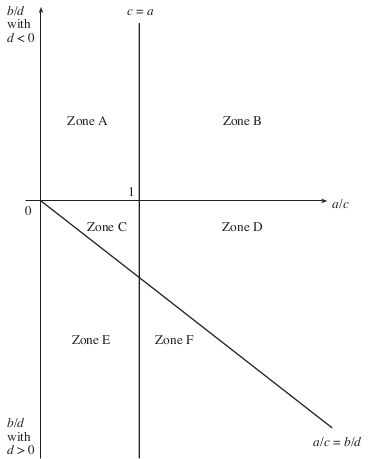
\includegraphics[scale=1]{market_plane_favereau.png}
		\fonte{\cite[p. 229]{favereau2002markets}}
	\end{figure}
	
	%To \citeonline{eloire2009reseaux}, the main goal of White's model is to show the structure of the market. The market plane shows six zones; four of them are zones that demarcate viable market, the other two, non-viable or unraveling. They can be described in a simplified way\footnote{A mathematical development of this plane is described in Appendix 1.} like this:
	
	Para \citeonline{eloire2009reseaux}, o principal objetivo do modelo de White é mostrar a estrutura do mercado. O plano do mercado mostra seis zonas; quatro delas são zonas que demarcam o mercado viável, as outras duas, o mercado não viável ou desvendado (\textit{unravelling}). Eles podem ser descritos de uma maneira simplificada da seguinte maneira:
	
	%Zone C is labelled \textbf{ordinary}. In this zone, revenues decrease to scale ($a/c < 1$) since cost increases with quality ($d > 0$). This is the `ordinary' that we think about quality. Also, returns are decreasing to quality to a more severe degree than to scale ($a/c > b/d$). Zones D and F are labelled \textbf{advanced}. In this zone higher quality is more expensive to produce ($d > 0$) and revenues increase to scale ($a/c > 1$). Zone A is labelled \textbf{paradox}. In this zone, in contrast with the ordinary thinking, higher quality is less costly to produce than lower quality ($d < 0$) although there are decreasing returns to scale ($a/c < 1$). B and E are non-viable market zones. 
	
	A zona C é chamada de \textit{ordinária}. Nessa zona, receitas diminuem com a escala ($a/c < 1$) visto que o custo aumenta com a qualidade ($d > 0$). Isto é o comum, o ``ordinário'', que pensamos sobre a qualidade. Além disso, os retornos diminuem com a qualidade em um grau mais severo do que com a escala ($a/c > b/d$). As zonas D e F são chamadas \textit{avançadas}. Nessa zona melhor qualidade é mais cara de ser produzida ($d > 0$) e as receitas aumentam com a escala ($a/c > 1$). A zona A é chamada \textit{paradoxo}. Nessa zona, em contraste com o pensamento ordinário, melhor qualidade é menos custosa de ser produzida do que pior qualidade ($d < 0$) embora os retornos diminuam com a escala ($a/c < 1$). B e E são zonas de mercado não viável.
	
	
	
	

	
	\subsection{Mensurações}
	
	%\subsubsection{Como o modelo $W(y)$ tem sido mensurado}
	
	%In the $W(y)$ model, measurements are an issue to be solved in a creative way because White does not close the scope of the variables to be chosen. The review of two important studies gives us a basis to decide on this measurement issue.
	
	No modelo $W(y)$, as mensurações são uma questão a ser resolvida de uma maneira criativa pois White não fecha o escopo das possíveis variáveis a serem escolhidas para isso. A revisão de dois estudos importantes nos dá uma base para decidir sobre a questão da mensuração.
	
	%\citeonline{biencourt2002market} studied the theatrical institutions markets. They argue that the main advantage of White's model is related to the interdependence of the market structure and individual decisions through niches. This is particularly interesting to this specific case because
	
	\citeonline{biencourt2002market} estudaram o mercado das instituições teatrais. Eles argumentam que a principal vantagem do modelo de White está relacionada à interdependência da estrutura do mercado e das decisões individuais através dos nichos. Isto é particularmente interessante porque
	
	\begin{citacao}
		Organizações teatrais baseiam a construção de seus nichos nas competências de seus times administrativo, técnico e artístico, nas experiências prévias do público e na política de elaboração dos programas que orienta as escolhas de repertório e diretores. O conceito de nicho é adequado à singularidade das performances. Sua qualidade é resultado de uma combinação da qualidade do trabalho individual dos atores e técnicos num projeto sob o controle do diretor\footnote{Theatrical organizations base their construction of niches on the competencies of their administrative, technical and artistic teams, the public's former experiences and the programming policy that orients choices of repertories and directors. The concept of a niche is suited to the uniqueness of performances. Their quality is the result of a combination of the quality of actors' and technicians' individual work on a project, under the control of the director.}. \cite[p. 255]{biencourt2002market}
	\end{citacao}
	
	
	%If we retake the functions of satisfaction (\ref{satisfaction}) and cost (\ref{cost}), the variables were chosen in this manner:
	
	Se retomarmos as funções de satisfação (\ref{satisfaction}) e custo (\ref{cost}), as variáveis foram escolhidas da seguinte maneira:
	
	\begin{itemize}
		\item \textbf{Volume de produção $Y$} -- estimado pelo número de performances listadas no relatório anual do teatro.
	\end{itemize}
	
	%The authors show that for \apudonline{throsby1993economics}{biencourt2002market} the number of tickets sold is a better suited indicator for $Y$. However, ``the determination of $S$ would then require one to know the degree of audience satisfaction after each performance, something that is impossible'' \cite[p. 264]{biencourt2002market}. The number of seats available for each performance would also have been a good indicator if the authors had access to this data.
	
	Os autores mostram que para \apudonline{throsby1993economics}{biencourt2002market} o número de ingressos vendidos é um indicador bem adequado para $Y$. Entretanto, ``a determinação de $S$ requereria que se conhecesse o grau de satisfação do público após cada performance, algo impossível\footnote{The determination of $S$ would then require one to know the degree of audience satisfaction after each performance, something that is impossible.}'' \cite[p. 264]{biencourt2002market}.  O número de assentos disponíveis para cada performance seria também um bom indicador se os autores tivessem acesso a esses dados.
	
	\begin{itemize}
		\item \textbf{Satisfação dos consumidores $S$} -- medida pelo número de visitantes pagantes à instituição.
	\end{itemize}
	
	%The authors justify this choice showing data from previous research on theatre audiences' habits and representations. Also, they divided the performances on four repertoire categories, namely, ``classical'', ``20th century'', ``contemporary French'' and ``contemporary foreign'' plays. They also make a correction for the repertory effect by ``multiplying the number of paying visitors observed  in each of the four categories by the average ratio $\bar{x}_i$ between the share of performances and that of the number of visitors in a given genre $i$ for all the institution markets'' \cite[p. 265]{biencourt2002market}. Let $\tilde{P}_i$ be the number of performances and $\tilde{V}_i$ be the number of paying visitors to all theatres in category $i$. The average can be defined by
	
	Os autores justificam essa escolha mostrando dados de pesquisas anteriores em hábitos do público do teatro e representações. Além disso, eles dividem as performances em quatro categorias de repertório, a saber, ``clássico'', ``século XX'', ``contemporâneo Francês'' e ``contemporâneo de outros países''. Eles também fazem uma correção para o efeito do repertório ``multiplicando o número de visitantes pagantes observados em cada uma das quatro categorias pela razão média $\bar{x}_i$ entre a proporção de performances e a proporção do número de visitantes em um dado gênero $i$ para todas as instituições do mercado\footnote{(\dots) Multiplying the number of paying visitors observed  in each of the four categories by the average ratio $\bar{x}_i$ between the share of performances and that of the number of visitors in a given genre $i$ for all the institution markets.}'' \cite[p. 265]{biencourt2002market}. Seja $\tilde{P}_i$ o número de performances e $\tilde{V}_i$ o número de visitantes pagantes para todos os teatros na categoria $i$. A média pode ser definida por
	
	\begin{equation}
	\label{repertory-effect-correction}
	\bar{x}_i = \frac{\tilde{P}_i / \sum_{i=1}^{4}\tilde{P}_i}{\tilde{V}_i / \sum_{i=1}^{4}\tilde{V}_i}	
	\end{equation}
	
	%If $v_i$ represents the number of paying visitors in category $i$ of repertoire, the public satisfaction can be estimated by
	
	Se $v_i$ representa o número de visitantes pagantes na categoria $i$ de repertório, a satisfação do público pode ser estimada por
	
	\begin{equation}
	\label{satisfaction-corrected}
	S = \sum_{i=1}^{4}\bar{x}_i v_i
	\end{equation}
	
	

	
	\begin{itemize}
		\item \textbf{O custo agregado $C$} -- esta variável foi obtida adicionando os custos artísticos do teatro (diferenciados aqui dos custos fixos).
		
		\item \textbf{escalar $r$} -- igual ao inverso do preço médio dos lugares $\bar{p}$ em todos os teatros.
		
		\item \textbf{escalar $q$} -- considerado igual a 1.
	\end{itemize}
	
	%Although White's model represents a big step in the construction of knowledge about the markets, it has an issue related to its very core, the quality ranking. To him, quality is given in a predetermined social space. In fact, \citeonline{favereau2002markets} states that to agree on price is not a big deal but to agree on quality is intrinsically a problem. We shall argue, however, that quality is not predefined but actors struggle and negotiate on a daily basis for its definition.
	
	Embora o modelo de White representa um grande passo na construção de conhecimento sobre os mercados, ele tem um problema relacionado com seu núcleo duro, o ranking de qualidade. Para ele, a qualidade é dada em um espaço social predeterminado. De fato, \citeonline{favereau2002markets} postulam que concordar no preço não é uma grande coisa mas concordar na qualidade é intrinsecamente um problema. Argumentamos, entretanto, que a qualidade não é predefinida mas que os atores disputam e negociam diariamente pela sua definição.
	
	%According to \citeonline{eloire2009reseaux}, by embracing the annual publications previously mentioned, this industry has ``specific judgement devices on quality'' as \citeonline{karpik2009elements}  argues. This devices do not only help the coordination between offer and demand, but they also ``contribuent au classement des producteurs selon des critères de qualité collectivement définis et surtout acceptés, mais qui sont aussi des objets de lutte pour leur définition'' \cite[p. 494]{eloire2009reseaux}. In fact, \citeonline{eloire2009reseaux} states that the very existence of various guides is, by itself, an evidence of this symbolic struggles for the definition of quality, although in the ``high distinction'' the guides seem to converge.
	
	De acordo com \citeonline{eloire2009reseaux}, ao receber as publicações anuais previamente mencionadas, esse setor tem ``dispositivos de julgamento específicos para a qualidade'' como argumenta \citeonline{karpik2009elements}. Estes dispositivos não somente ajudam a coordenação entre oferta e demanda mas também ``contribuem à classificação dos produtores de acordo com os critérios de qualidade definidos coletivamente e sobretudo aceitos, mas que são também objetos de luta por definição\footnote{(\dots) Contribuent au classement des producteurs selon des critères de qualité collectivement définis et surtout acceptés, mais qui sont aussi des objets de lutte pour leur définition.}'' \cite[p. 494]{eloire2009reseaux}. De fato, \citeonline{eloire2009reseaux} postula que a própria existência de vários guias de qualidade é, em si, uma evidência dessa luta simbólica pela definição da qualidade, embora na ``alta distinção'' os guias tendam a convergir.
	
	%What if there are no guides or websites to testify on orchestra's quality and the critics in the main newspapers in town are nearly nonexistent? Well, this is the case in Belo Horizonte and it poses a quite of a challenge. All the cultural economics and singularities economics discussion on quality relies on the action of critics who are, per excellence, the ones who have the primacy of quality definition. In Belo Horizonte, orchestral performances almost never get a critic and there is not such a well structured platform for it as Rotten Tomatoes\footnote{\url{https://www.rottentomatoes.com}.} or \textit{Adoro Cinema}\footnote{A famous Brazilian movie critics website. Available in \url{http://www.adorocinema.com}.} for movies. If critics do not act much within the field of our study object, where does the quality definition come from?
	
	E se não houverem guias ou plataformas online especializadas para testificar da qualidade de uma orquestra e a presença de críticas nos jornais for ínfima? Este é o caso da cidade de Belo Horizonte, MG, e ele coloca um grande desafio à pesquisa. Toda a discussão da economia da cultura e da economia das singularidades sobre a qualidade repousa sobre uma ação dos críticos que são, por excelência, aqueles que possuem a primazia da definição da qualidade. Em Belo Horizonte as performances orquestrais quase nunca recebem uma crítica e não há uma plataforma bem estruturada para isso como o Rotten Tomatoes\footnote{\url{https://www.rottentomatoes.com}.} ou \textit{Adoro Cinema}\footnote{Um website brasileiro famoso de críticas de cinema. Disponível em \url{http://www.adorocinema.com}.}. Se as críticas não possuem grande atuação dentro do campo de nosso objeto de estudo, de onde vem a definição da qualidade?
	
	%\citeonline{biencourt2002market} present an interesting approach to the quality problem regarding theatres' market. We shall depart from their rationale to build the quality index $n$ we will use in this investigation.
	
	\citeonline{biencourt2002market} apresentam uma abordagem interessante para o problema da qualidade com relação ao mercado teatral. Partiremos de sua \textit{rationale} para construir o índice de qualidade $n$ que usaremos em nossa investigação.
	
	%To deal with quality index $N$, the authors elaborate a sophisticated construct to explain how various actors have a different influence on quality. To them,
	
	Para lidar com o índice de qualidade $N$, os autores elaboraram um construto sofisticado para explicar como vários atores tem diferentes influências sobre a qualidade. Para eles
	
	\begin{equation}
	\label{biencourt-quality}
	N_{l}^{b_l} = N_{1l}^{b_{1l}} N_{2l}^{b_{2l}} N_{3l}^{b_{3l}} N_{4l}^{b_{4l}} 
	\end{equation}
	
	%that is, the \textit{overall quality} $N$ in the year $l$ is constructed aggregating the judgements of \textit{drama critics} $N_1$, the judegements of \textit{programme planners} $N_2$, the judgement of the \textit{public authorities} $N_3$ and the influence of \textit{previous consumption} $N_4$. Now, each of these parts of the overall quality were measured in this manner:
	
	isto é, a \textit{qualidade geral} $N$ no ano $l$ é construída agregando as opiniões de \textit{críticos de teatro} $N_1$, as opiniões de \textit{planejadores de programas} $N_2$, a opinião de \textit{autoridades públicas} $N_3$ e a influência de \textit{consumo prévio} $N_4$. Cada uma das partes da qualidade geral foi mensurada da seguinte maneira:
	

	
	\begin{itemize}
		\item \textbf{Opiniões de críticos teatrais $N_1$} -- mensuradas registrando todas as críticas de apresentações agendadas nos teatros nos jornais \textit{Le Monde} e \textit{Libération} e na revista \textit{Télérama}, líderes de opinião entre os críticos teatrais.

		\item \textbf{Opiniões dos planejadores de programas $N_2$} -- a centralidade de grau de entrada normalizada do teatro; nesse caso, isso significa o número de performances de espetáculos produzidos por outras instituições teatrais agendadas pelo teatro divididas pela centralidade máxima da rede.
		
		\item \textbf{Opiniões de autoridades públicas $N_3$} -- mensurada pelo volume de subsídio do Estado. Para \citeonline[p. 267]{biencourt2002market}, ``essa escolha é justificada pelo peso do Estado que é maior do que o das autoridades locais no reconhecimento político da reputação de uma instituição artística\footnote{This choice is justified by the weight of the state, which is greater that that of local authorities in the political recognition of an institution's artistic reputation.}''.

		\item \textbf{Influência de consumos prévios $N_4$} -- mensurada pelo número de visitantes pagantes no período precedente.
	\end{itemize}
	
	%The overall quality perceived by the public is constructed by aggregating these four variables in the form of a Cobb-Douglas function (cf. equation \ref{biencourt-quality}). To measure the weight of each one of these variables on the overall quality, they estimated a linear model that had the number of paying visitors per performance as the dependent variable. Knowing that $r = 1/\bar{p}$ and taking into account equations (\ref{satisfaction}) and (\ref{biencourt-quality}), we can derive
	
	A qualidade geral percebida pela público é construída agregando essas quatro variáveis na forma de uma função Cobb-Douglas (cf. equação \ref{biencourt-quality}). Para medir o peso de cada uma das variáveis, eles estimaram um modelo linear que possuía o número de visitantes pagantes por performances como variável dependente. Sabendo que $r = 1/\bar{p}$ e levando em conta as equações (\ref{satisfaction}) e (\ref{biencourt-quality}), podemos derivar
	
	\begin{equation}
	\label{biencourt-derivation}
	[S\bar{p}/Y]_l = Y_{l}^{\hat{a}_l} N_{l}^{\hat{b}_l} \varepsilon_l = Y_{l}^{\hat{a}_l} N_{1l}^{\hat{b}_{1l}} N_{2l}^{\hat{b}_{2l}} N_{3l}^{\hat{b}_{3l}} N_{4l}^{\hat{b}_{4l}} \varepsilon_l
	\end{equation}
	
	%where $l$ is the year under investigation. This leads to the linear model
	onde $l$ é o ano sob investigação. Isso leva ao modelo linear
	
	\begin{equation}
	\label{regression}
	\log([S\bar{p}/Y]_l) = \hat{a}_l \log Y_l + \hat{b}_{1l} \log N_{1l} + \hat{b}_{2l} \log N_{2l} + \hat{b}_{3l} \log N_{3l} + \hat{b}_{4l} \log N_{4l} + \hat{\varepsilon}_l
	\end{equation}
	
	%From this, it is possible to deduce, without a constant,
	Disto é possível deduzir, sem a constante,
	
	\begin{equation}
	\label{N-com-pesos}
	\log N_l = \hat{b}_{1l} \log N_{1l} + \hat{b}_{2l} \log N_{2l} + \hat{b}_{3l} \log N_{3l} + \hat{b}_{4l} \log N_{4l} + e_l \hat{\varepsilon}_l
	\end{equation}
	
	%with $0 \le e_l \le 1$ assuming $\hat{b}_l = 1$.
	com $0 \le e_l \le 1$ assumindo $\hat{b}_l = 1$.
	
	%Then, the four elasticities exponents were deduced as solutions of a system of two equations to two unknowns. As the authors were studying two years seasons, by posing $\Delta = \log Y_l \cdot \log N_{l+1} - \log Y_{l+1} \cdot \log N_l$, they obtain:
	
	Então, os quatro expoentes de elasticidade foram deduzidos como soluções de um sistema de duas equações para dois desconhecidos. Como os autores estudaram duas temporadas, definindo $\Delta = \log Y_l \cdot \log N_{l+1} - \log Y_{l+1} \cdot \log N_l$, eles obtiveram:
	
	$$ a = \frac{ \log([S\bar{p}]_l) \cdot \log N_{l+1} - \log([S\bar{p}]_{l+1}) \cdot \log N_{l} }{\Delta} $$
	
	$$ b = \frac{ \log([S\bar{p}]_{l+1}) \cdot \log Y_{l} - \log([S\bar{p}]_{l}) \cdot \log Y_{l+1} }{\Delta} $$
	
	$$ c = \frac{ \log C_l \cdot \log N_{l+1} - \log C_{l+1} \cdot \log N_{l} }{\Delta} $$
	
	\begin{equation}
	\label{parameters}
	d = \frac{ \log C_l \cdot \log Y_{l+1} - \log C_{l+1} \cdot \log Y_{l} }{\Delta}
	\end{equation}
	
	

	
	% OBS: A partir da página 280, Éloire começar a falar dos niches de qualités e as variáveis que escolhe para medir cada parte do modelo.
	
	%On the other hand, \citeonline{eloire2009reseaux} chose a different set of variables to measure the inputs of the $W(y)$ model. In his PhD thesis, he studied the market of restaurants in Lille. He also uses the number of clients as an indicator to $y$ and observes the revenues (\textit{Chiffre d'affaires}) as well as uses the average ticket price for $W$. In order to investigate the market plane, \citeonline{eloire2009reseaux} mobilized the variables described in Table \ref{eloire-abcd}:
	
	Por outro lado, \citeonline{eloire2009reseaux} escolheu um set diferente de variáveis para medir os \textit{inputs} do modelo $W(y)$ Em sua tese de doutoramento, ele estudou o mercado dos restaurantes em Lille (França). Ele também usou o número de clientes como indicador de $y$ e observa as receitas (\textit{Chiffre d'affaires}) e o preço médio da entrada para $W$. Para investigar o plano do mercado, \citeonline{eloire2009reseaux} mobilizou as variáveis descritas na Tabela \ref{eloire-abcd}:
	
	\begin{table}[ht]
		\ibgetab{
			\centering
			\caption{Parâmetros de nichos de qualidade}
			\label{eloire-abcd}
		}
		{\begin{tabular}{c | p{5cm} p{5cm}}
				\hline
				& \textbf{Volume}  & \textbf{Qualidade} \\
				\hline
				\textbf{Satisfação}  & \textbf{a} = Número médio de clientes por serviço & \textbf{b} = Valor médio da entrada + Nota da qualidade \\
				\textbf{Custo} & \textbf{c} = Assalariados / \textit{Couverts} * Serviços & \textbf{d} = Razão de disponibilidade de assalariados / clientes \\
				\hline
			\end{tabular}
		}
		{\fonte{\citeonline[p. 289]{eloire2009reseaux}}}
	\end{table}




	% This here is on page 290!!!
	%Éloire argues that quality is a social construction build between the offer from structured producers and an aggregated demand. In the restaurants case, it also depends on the ``cuisine'' style which is very difficult to measure. However, this culinary scale is closely correlated with simple economic statistics: price, availability ratio in a way that the higher the prices and the ratio, the more ``fancy'' is the restaurant. Therefore, he considers the quality cost (\textbf{d} parameter) is related to the availability ratio, that is the amount of personnel that a restaurant hires over the number of clients it intends to serve. Clients satisfaction (\textbf{b} parameter) can be represented by the average ticket value.
	
	Éloire argumenta que a qualidade é uma construção social feita entre a oferta de produtores estruturados e a demanda agregada. No caso dos restaurantes, isso também depende do estilo de \textit{cuisine} o qual é bastante difícil de mensurar. Entretanto, essa escala culinária está fortemente correlacionada com estatísticas econômicas simples: preço, taxa de de disponibilidade de modo que quanto maior os preços e a taxa, mais ``\textit{chic}'' é o restaurante. Portanto, ele considera que o custo de qualidade (o parâmetro \textbf{d}) está relacionado com a razão de disponibilidade, isto é, a quantidade de pessoal que o restaurante contrata sobre o número de clientes que ele intenciona servir. A satisfação da clientela (o parâmetro \textit{b}) pode ser representado pelo valor médio do ticket.
	
	% PAGE 290
	%The author recognizes that the a restaurant's capacity is correlated to the volume of personnel. So, the volume costs (\textbf{c} parameter) are measured to the number of salaried employees divided by the (potential) number of cutlery multiplied by the number of services. Also, he acknowledges that a main strategy of the restaurants is related to the amount of time/time of the day that it stays open. Some restaurants can function 24/7, some only at lunch, some only at night,  and this implicates requires cost, personnel, logistics, etc. This is expressed on the \textbf{c} parameter calculus. The satisfaction at volume (\textbf{a} parameter) is measured by the average number of clients per service. This is derived of the restaurant's ``filling rate''. The higher this rate, the more we can infer that his decisions regarding volume costs are validated by the clients. On the other hand, the lower this rate, the more the volume costs can be seen as ``disproportional'' by the clients \cite{eloire2009reseaux}.
	
	O autor reconhece que a capacidade de um restaurante está correlacionada com o volume de pessoal. Portanto, o volume de custos (o parâmetro \textbf{c}) é medido pelo número de empregados assalariados dividido pelo número (potencial) de talheres multiplicado pelo número de serviços. Ainda, ele percebe que a principal estratégia dos restaurantes está relacionada com a quantidade de time/a hora do dia em que ele permanece aberto. Alguns restaurantes podem funcionar 24hs, alguns apenas no horário de almoço, outros apenas à noite, e isso implica custos, pessoal, logística, etc. Isto é expresso no cálculo do parâmetro \textbf{c}. A satisfação quanto ao volume (o parâmetro \textbf{a}) é medida pelo número médio de clientes por serviço. Isto é derivado da ``taxa de lotação'' do restaurante. Quanto maior a taxa, mais é possível inferir que suas decisões quanto aos custos de volume são validadas pelos clientes. Por outro lado, quanto menor a taxa mais os custos de volume podem ser vistos como ``desproporcionais'' pelos clientes \cite{eloire2009reseaux}.
	
	%The quality note pointed by the author in table \ref{eloire-abcd} is built aggregating the notes of five international restaurant guides, all of them well known and recognized in the profession, namely, ``Le Guide Michelin France'', ``Le Bottin Gourmand'', the ``GaultMillau'', the ``Champérard'' and ``Le Pudlo France''. The aggregation of these guides scoring was obtained through a specialized website\footnote{\url{http://restaurant-hitlisten.de/france/bewertung.htm}}.
	
	A qualidade da nota apontada pelo autor na tabela \ref{eloire-abcd} é construída agregando as notas de cinco guias internacionais de restaurantes, todos muito bem conhecidos e reconhecidos na meio profissional, a saber, ``Le Guide Michelin France'', ``Le Bottin Gourmand'', o ``GaultMillau'', o ``Champérard'' e ``Le Pudlo France''. A agregação das notas desses guias foi obtida através de um site especializado\footnote{\url{http://restaurant-hitlisten.de/france/bewertung.htm}}.
	
	
	
% \begin{comment}

% 	%\subsection{Nossa proposta de mensuração}
	
	
% 	Retomemos as duas principais equações do modelo $W(y)$. Primeiro a equação de custo (\ref{cost}):
% 	$$C(y, n) = q \cdot y^c \cdot n^d$$
% 	e a equação de satisfação (\ref{satisfaction}):
% 	$$S(y, n) = r \cdot y^a \cdot n^b$$
	
% 	Para os propósitos desta investigação os parâmetros serão mensurados da seguinte maneira:
	
% 	\begin{itemize}
% 		\item A constante $q = 1$;
% 		\item A constante $r =$ o inverso do preço médio do ingreso nas performances da temporada, isto é, $1/\bar{p}$;
% 		\item O custo agregado $C$ será obtido pelos custos artísticos da orquestra;
% 		\item A satisfação do público $S$ será estimada pela razão entre o número de indivíduos pagantes no público sobre o número de assentos;
% 		\item O volume de produção $y$ será estimado pelo número de assentos disponíveis para cada performance\footnote{Caso não tenhamos acesso a esse dado, $y$ será estimado pelo número total de performances na temporada.};
% 		\item O índice de qualidade $n$ será estimado agregando o preço do ticket, o orçamento total, ``proximidade com o Estado'' e a percepção dos músicos;
% 		\item ``A proximidade com o Estado'' será mensurada pelo número de contratos assinados e o financiamento total proveniente do Estado.
% 	\end{itemize}
	
	
% 	%The elasticities $a$ and $b$, related to the Satisfaction equation, can be obtained as solutions of a system of two equations to two unknowns as proposed by \citeonline{biencourt2002market}. Trying to measure any of these variables would violate the assumption that cultural goods are not rivals in consumption.
	
% 	As elasticidades $a$ e $b$, relacionadas à equação de satisfação, podem ser obtidas como soluções de um sistema de duas equações para dois desconhecidos como proposto por \citeonline{biencourt2002market}. Tentar medir algumas dessas variáveis violaria o pressuposto de que bens culturais não são rivais no consumo.
	
% 	%The elasticities $c$ and $d$, on the other hand, can be measured in the following way:
% 	% ELABORATE! ELABORATE! ELABORATE! ELABORATE! ELABORATE!
	
% 	As elasticidades $c$ e $d$, por outro lado, podem ser mensuradas da seguinte maneira:
	
% 	\begin{itemize}
% 		\item $c =$ o número de empregados assalariados  $/$ número de performances;
% 		\item $d =$ orçamento total $/$ número de performances.
% 	\end{itemize}
	
% 	A tabela \ref{measurements-wy} sintetiza as variáveis escolhidas como indicadores para medir os \textit{inputs} do modelo $W(y)$.
	
% 	\begin{table}
% 		\ibgetab{
% 			\caption{Indicadores propostos - modelo $W(y)$}
% 			\label{measurements-wy}
% 		}
% 		{\begin{tabular}{|c|c|}
				
% 				\hline
% 				\textbf{Conceito} & \textbf{Indicador} \\
% 				\hline
% 				A constante \textbf{q} & 1 \\
% 				\hline
% 				A constante \textbf{r} &  $1/\bar{p}$ \\
% 				\hline
% 				Custo agregado \textbf{C} & Despesas artísticas \\
% 				\hline
% 				Satisfação \textbf{S} & Indivíduos pagantes / assentos à disposição \\
% 				\hline
% 				Volume de produção \textbf{y} & Assentos disponíveis (ou número de performances) \\
% 				\hline
% 				Índice de qualidade \textbf{N} & Preço do ingresso, \\
% 				& Orçamento total, \\
% 				& ``Proximididade com o Estado'', \\
% 				& Precepção dos músicos. \\
% 				\hline
% 				``Proximidade com o Estado'' & Número de contratos assinados, \\
% 				& Financiamento total do Estado. \\
% 				\hline
% 				A elasticidade \textbf{c} & Número de empregados / número de performances \\
% 				\hline
% 				A elasticidade \textbf{d} & Orçamento total / número de performances\\
% 				\hline
% 			\end{tabular}
% 		}
% 		{\fonte{Elaborado pelo autor.}}
% 	\end{table}

% \end{comment}	




        \subsection{Algumas considerações sobre a teoria}

        Muito embora o modelo $W(y)$ possua uma formulação que lembre bastante os construtos elegantes da área econômica, ele possui um elemento sociológico por excelência em sua essência, a saber, a noção de que os mercados não são estruturas dadas mas emergem das relações entre organizações. ...





        

	\section{A arquitetura dos mercados}

	Neil \citeonline{fligstein2002architecture} traça uma teorização sobre a emergência e funcionamento dos mercados ligeiramente diferente da que vimos em White. Fligstein também leva em conta uma estrutura relacional onde firmas interagem entre si e com o comprador generalizado visando a estabilização do mercado (e consequente subsistência de todos). A grande diferença fica por conta da participação do Estado. Enquanto White não tece grandes considerações acerca do papel estatal na emergência e funcionamento dos mercados de produção, Fligstein elabora seu esquema teórico identificando a estrutura do Estado como central para o desenvolvimento dos mercados. Por que Estados? - pergunta Fligstein. O próprio autor responde que ``À medida que a possibilidade de padrões de interação complexos na esfera da troca econômica se expandem, os atores se mostraram incapazes de prover regras para si mesmos\footnote{As the possibility for complex patterns of interaction in the sphere of economic exchange has expanded, actors have proven incapable of providing rules for themselves.}'' \cite[p. 27-8]{fligstein2002architecture} e, portanto, recorrem ao Estado como provedor de regras para que o jogo econômico funcione de maneira justa.

	\citeonline{fligstein2002architecture} concebe os mercados como ``campos'', arenas sociais onde vendedores e compradores se encontram. Essas arenas obedecem a quatro tipos puros de regras para a produção e reprodução de sua estrutura, quais sejam:

	\begin{enumerate}
		\item direitos de propriedade;
		\item estruturas de governança;
		\item regras de troca e
		\item concepções de controle.
	\end{enumerate}

	Estas diferentes formas de regulação são inclusivas; o nível posterior necessariamente pressupõe o anterior. Do primeiro ao último há um maior grau de generalidade.

	Direitos de propriedade são, segundo o autor, regras que definem quem possui diretos sobre os retornos financeiros das firmas. Formas comuns de direito de propriedade são patentes e credenciais. Sua constituição não é, necessariamente, o desfecho de um processo eficiente mas um contínuo e contestável processo político \cite{fligstein2002architecture}.

	Essa regras configuram condição \textit{sine qua non} de existência de mercados uma vez que definem as relações entre aqueles que detém posse de algum bem e os demais estabilizando o mercado. ``Os direitos de propriedade funcionam, portanto, para produzir duas formas de estabilidade: a definição de relações de poder entre constituintes dentro e fora das firmas e sinalizar a outros quem essas firmas são\footnote{Property rights thus function to produce two forms of stability: defining the power relationships between constituencies in and around firms, and signaling to other firms who firms are.}'' \cite[p. 34]{fligstein2002architecture}.

	Estruturas de governança são estruturas de regras gerais ao nível da sociedade que definem relações competitivas e cooperativas entre firmas além de sua organização interna. Essas regras definem formas legais e ilegais de controle da competição no espaço mercantil. Elas podem aparecer na forma de leis (e.g., leis antitrustes) ou normas sociais muito embora assumam grande variação entre diferentes sociedades. Cabe ressaltar que a organização interna de uma firma também se dá como resposta a formas legais ou ilegais de competição no mercado. Firmas podem se integrar tanto verticalmente, como forma de assegurar seus insumos necessários, quanto horizontalmente, comprando ações visando produzir um ordenamento estável no mercado ou diversificando sua carta de produtos visando proteção contra os ``caprichos de produtos específicos'' \cite[p. 34]{fligstein2002architecture}. A formação de parcerias estáveis e de longo prazo também configuram respostas à competição.

	As regras de troca definem quem pode se engajar em transações comerciais com quem bem como suas condições. As regras abrangem pesos, padrões comuns, fretagem, cobrança, seguro, trocas financeiras e a firma de contratos. ``As regras de troca ajudam a estabilizar os mercados assegurando que as trocas ocorram sob condições que se aplicam a todos\footnote{Rules of exchange help stabilize markets by ensuring that exchanges occur under conditions that apply to everyone.}'' \cite[p. 35]{fligstein2002architecture}. Alguns dos tratados comerciais internacionais mais recentes como o GATT (\textit{General Agreement of Tariffs and Trade}) focam na harmonização das regras de troca.

	``Concepções de controle refletem acordos específicos de mercado entre atores em firmas sobre princípios de organização interna (\dots), táticas de competição ou cooperação (\dots), e a hierarquia ou o ordenamento de status das firmas num dado mercado\footnote{Conceptions of control reflect market-specific agreements between actors in firms on principles of internal organization (\dots), tactics for competition or cooperation (\dots), and the hierarchy or status ordering of firms in a given market.}'' \cite[p. 35]{fligstein2002architecture}. São, em sua essência, produtos histórico-culturais. São históricos à medida que se restringem ao contexto histórico de um determinado setor em uma determinada sociedade e são culturais pois formam um arcabouço de entendimentos e práticas vigentes num dado mercado. Para \citeonline{fligstein2002architecture}

	\begin{citacao}
		Um mercado estável é um campo social no qual a concepção de controle define as relações sociais entre firmas vendedoras incumbentes e desafiantes de modo que as incumbentes reprodruzem essas relações de tempos em tempos. O propósito da ação em um dado mercado é criar e manter mundos estáveis dentro das firmas e entre elas que permita a sobrevivência de firmas dominantes\footnote{A stable market is a social field in which a conception of control defines the social relations between incumbent and challenger seller firms such that the incumbent firms reproduce those relations on a period-to-period basis. The purpose of action in a given market is to create and maintain stable worlds within and across firms that allow dominant seller firms to survive.}. \cite[p. 35]{fligstein2002architecture}
	\end{citacao}

	As concepções de controle evidenciam também, como podemos notar, um elemento político dos mercados no que toca à manutenção do ordenamento hierárquico vigente, sua reprodução e sua manifestação no processo de definição de padrões de qualidade e certificação. Dito de outra forma, as concepções de controle colocam perguntas como ``quem controla a entrada e saída de um sistema concorrencial?'' ``Como os desafiadores e os dominantes entram em relação?'' ``Quem consegue impor a pauta de qualidade num setor industrial, por exemplo, um \textit{standard} ISO ou um sistema de certificação do que é um produto orgânico no mercado de alimentos?''

	Para Fligstein, a entrada de países em sistemas capitalistas ``empurra'' os Estados a uma posição regulatória com relação aos quatro tipos acima mencionados. No exercício regulatório, os Estados produzem normativas culturais que determinam o processo de estruturação da ação econômica. Esse exercício é contínuo. Constantemente os Estados lidam com situações de crise e com o \textit{lobby} das empresas clamando por intervenção estatal. Os rumos que os mercados tomam estão diretamente relacionados a dois fatores: (1) a capacidade de intervenção, regulação e mediação do Estado e (2) o poder de organizações privadas para influenciar os termos de intervenção.

	O Estado tem ainda um papel fundamental no financiamento da inovação. Segundo \citeonline{fligstein2002architecture}

	\begin{citacao}
		Os governos nas sociedades industriais tem um papel importante quanto ao investimento e mediação da luta de classe. As ações dos empresários e empreendedores são enquadradas em torno dessas formas de estabilidade. Eles podem criar novos setores usando a ajuda do governo para investir em tecnologias arriscadas. Eles podem diversificar os riscos em suas firmas para produzir identidades estáveis para as firmas\footnote{Governments in industrial societies play a role in investment and mediating the class struggle as well. The actions of managers and entrepreneurs are framed around these forms of stability. They can create new industries using government support to invest in uncertain technologies. They can diversify their risks in their firms to produce stable identities for firms.}. \cite[p. 62]{fligstein2002architecture}
	\end{citacao}

	Para esse autor, seria muito difícil imaginar a existência de um mercado sem o aparato estatal cuidando de seu regulamento e estabilização. Isso, entretanto, não implica que a atuação estatal seja neutra mas ela reproduz o controle de grupos sociais dominantes os quais mantém uma relação próxima do Estado e tem primazia nos pedidos de intervenção em épocas de crise. Sem as regras e acordos geridos pelo Estado, não haveria uma organização-social mínima para que produtores possam arriscar com novos produtos fazendo emergir novos mercados.

	Para Fligstein, num mercado o preço é um indicador confiável de qualidade. As empresas se veem impelidas pela competição de preços a diferenciar seus produtos formando nichos como forma de proteção contra a instabilidade. A diversificação da carta de produtos é também uma estratégia dominante para a diminuição de riscos. ``Uma firma pode produzir produtos múltiplos que reduzem sua dependência em um produto específico e, portanto, aumenta suas chances de sobrevivência\footnote{A firm can produce multiple products that reduce their dependence on any one product and, hence, increase the likelihood that the firm will survive.}'' \apud[p. 74]{kay1997pattern}{fligstein2002architecture}.

	\citeonline[p. 81]{fligstein2002architecture} postula ainda que ``em mercados com concepções de controle estáveis, os participantes amplamente concordam com a concepção de controle, com a hierarquia de status e as estratégias que ela implica\footnote{In markets with stable conceptions of control, market participants widely agree on the conception of control and the status hierarchies and strategies it implies.}''. Uma vez estabilizado, o mercado é compreendido tanto por firmas estabelecidas como ``desafiantes'' em sua estrutura de poder. Essa estrutura permite a avaliação da ação e das estratégias das firmas por qualquer observador e, consequentemente, sua ação orientada sobre essas estratégias. Aqui, estamos muito próximos ao que White chama de ``disciplina'' do mercado.

	As crises nos mercados são percebidas quando firmas estabelecidas começam a falir. Isso pode ser causado por três eventos: (1) queda na demanda pelo produto o que pode ser proveniente de más condições econômicas ou mudanças nas preferências dos compradores, (2) a entrada de uma nova firma no mercado distorcendo a concepção de controle vigente e forçando a reorganização do mercado ou (3) o Estado pode, intencionalmente ou não, mudar as regras vigentes e desestabilizar o mercado.

	É curioso notar que enquanto para Fligstein o Estado tem um papel preponderante na estrutura de mercado, para White o Estado não conta com a mesma importância. Sua teoria é construída nas relações entre firmas, em sua capacidade de percepção do tecido relacional que compõe a estrutura do mercado e na diferenciação de hierarquias por qualidade. Ambos os autores também divergem quanto à postura de cada firma em relação a seu posicionamento no mercado. Para White, a busca pelo posicionamento ótimo advém da observação dos pares engajamentos/retornos. A hierarquização das firmas (e consequente estabilização do mercado numa interface inteligível por todos) se dá por meio da qualidade percebida. Já para Fligstein, a busca pelo posicionamento se dá através de estratégias de proteção contra a concorrência dos preços (construção de nichos de mercado), da diversificação da carta de produtos oferecidos num ambiente que visa a estabilidade onde a figura central de controle é o Estado.

	A abordagem de Fligstein, como vimos, dá um papel central ao Estado como articulador, regulador e estabilizador do mercado. Sem ele, a estrutura não teria condições para fazer emergir uma normativa compartilhada que servisse como regime de controle, solo sólido para orientação da ação econômica e elaboração de estratégias de atuação. Estamos falando do clássico problema da ação coletiva; ela se preocupa em barrar a atuação de ``caronas'' e alocar de forma equânime custos de produção de bens públicos. Como podemos pensar num mercado, uma estrutura concorrencial por excelência, como uma ação coletiva? Ocorre cooperação? De fato, para que o mercado se estabilize e haja distribuição igualitária de oportunidades e acesso ao mercado tanto por firmas dominantes quanto desafiantes, em alguma medida  elas acabam cooperando mesmo que essa cooperação ocorra em um nível supraintencional. Isso se assemelha ao famoso conceito da ``mão invisível'' de Adam Smith. O trabalho do sociólogo seria, portanto, torná-la visível.

	%Resta ainda uma investigação mais profunda sobre o processo de atuação das firmas no dia a dia engajando-se em movimentos ao mesmo tempo de competição e cooperação. O conceito de isomorfismos organizacionais parecem lançar uma boa luz sobre esses processos. Vejamo-los mais detidamente.



	
	\section{A busca de nichos como processo social regulatório}

	Para \citeonline{lazega2009theorie}, a busca das firmas pela estabilização de um mercado passa por uma noção de qualidade construída coletivamente a partir das relações tecidas pelas firmas. Em sua atuação, as firmas se engajam em processos ao mesmo tempo de competição e cooperação -- o que ficou conhecido na sociologia das organizações como \textit{coopetition}. As organizações não conduzem seus negócios de maneira isolada mas são necessariamente dependentes de alguns recursos que as forçam a tecer laços de cooperação com outras organizações. Essas relações podem se manifestar na forma de um quadro jurídico e social mais ou menos definido. Segundo o autor, ``esses recursos interorganizacionais trocados através de laços multiplexos, podendo consistir de aprendizado, bens ou serviços, não são forçosamente de natureza monetária ou puramente funcional\footnote{Ces resources interorganisationnelles, échangés à travers des liens multiplexes, et pouvant consister en de l'apprentissage, des biens, des services, ne sont pas forcément de nature monétaire ou purement fonctionnelle.}'' \cite[p. 568]{lazega2009theorie}.

	Em sua atuação, o empreendedor busca a estruturação de seu contexto de interações e de negócios visando a sua própria segurança no mercado e a de seus investimentos relacionais. Esse processo, que possui uma forte capacidade de politização, leva o empreendedor a uma autorestrição contextual quanto à seleção de seus parceiros comerciais. Segundo o autor

	\begin{citacao}
	A troca social conduz o empreendedor a uma forma de autodisciplina social que se apoia de fato sobre uma endogeneização (\dots) das estruturas relacionais. Essa endogeneização toma a forma de manutenção ou construção de nichos sociais bem como de entrada na concorrência por status social\footnote{L'échange social conduit ainsi l'entrepreneur à une forme d'autodiscipline sociale qui s'appuie en fait sur une endogénéisation (\dots) des structures relationnelles. Cette endogénéisation prend la forme de l'entretien ou de la construction de niches sociales ainsi que celle d'une entrée dans la concurrence de statut social.}. \cite[p. 572]{lazega2009theorie}
	\end{citacao}

	A busca por nichos sociais, desse modo, é um primeiro meio de mobilização de uma estrutura de oportunidades. O nicho social, portanto, pode ser definido como o ``subconjunto de colegas-concorrentes com os quais se tem relações especialmente densas, multifuncionais, duráveis e ligadas, direta ou indiretamente, a suas atividades de produção\footnote{(\dots) le sous-ensemble de collègues-concurrents avec lesquels il/elle a des relations spécialement denses, multifonctionnelles, durables et liées, directement ou indirectement, à ses activités de production.}'' \cite[p. 575]{lazega2009theorie}.

	Na estruturação do tecido social que compõe o mercado processos sociais se articulam com disciplinas sociais emergentes proporcionando uma estrutura cognitiva pela qual pode-se orientar a ação econômica. Nessa articulação, quatro processos sociais se engajam com disciplinas:

	\begin{enumerate}
		\item Apredizado coletivo;
		\item Fenômenos de solidariedade;
		\item Controle social e
		\item Regulação e institucionalização.
	\end{enumerate}

	De maneira bastante breve, o aprendizado coletivo ou aprendizado organizacional ocorre a partir de fluxos de informações, recursos (humanos ou materiais) e através de trocas de conhecimento tácito. Fenômenos de solidariedade podem ocorrer na presença de ameaças ou instabilidade no mercado. Acordos comerciais, coletivos, associações entre empresas que, embora concorrentes, cooperam, emergem como estratégia de conquista de espaço no campo social. O controle social é facilitado pelos nichos sociais e pelo reconhecimento de uma estrutura de status entre organizações. Por fim, processos de regulação e institucionalização consistem da redefinição das regras do jogo. Nesse processo, organizações competem e cooperam para estabelecer uma linguagem de referência, um corpo normativo comum.
	
	%Our research aims to investigate a social regulatory process par excellence: the construction of the quality standard. As we saw, the quality index is the main gear that makes the orchestral music market engine run. The emergence of quality is a regulatory process that comes out of a struggle between the various actors involved in the market (musicians, public, critics, the State). The outcome would not necessarily be defined in terms of which actor is the most powerful, as conventional sociological theory would state, but it will emerge as a construct from complex interactions of \textit{coopetition} movements of the actors.
	
	Nossa pesquisa está interessada em investigar um processo social regulatório por excelência: a construção do padrão de qualidade. Como vimos, o índice de qualidade é a principal engrenagem que faz o motor do mercado da música de concerto funcionar. A emergência de qualidade é um processo regulatório que emerge de uma disputa entre vários atores envolvidos no mercado (músicos, público, crítica, o Estado). O resultado não seria necessariamente definido em termos de investigar qual ator detém mais poder, como a teoria sociológica convencional colocaria, mas emerge como um construto de interações complexas de movimentos de \textit{coopetição} entre os atores.
	
	\section{Isomorfismos normativos}

	Ao se debruçar sobre o mesmo fenômeno, a estruturação do campo de um mercado, \citeonline{dimaggio1983iron} mobilizam o conceito de isomorfismo para dar conta dos processos de competição-cooperação nos quais as organizações se engajam. Esses autores partem da seguinte pergunta: Por que as organizações são tão parecidas? Embora a pergunta pareça trivial, ela não é de nenhum modo intuitiva. A questão está em diálogo com um diagnóstico amplo da sociologia weberiana em relação à crescente racionalização do mundo industrial. Ora, se nos mercados a ação racional é concorrencial, esperaríamos que houvesse maior diversificação das formas organizacionais, cada uma buscando meios diferentes de subsistência. Não é o que os autores percebem ao postular a questão supracitada. %verificar isso com o Silvio

	Uma vez que organizações diversas se engajam numa mesma linha de mercado formando um estrutura (um campo), os processos que levam à similaridade começam a emergir com robustez.

	De que falamos, entretanto, quando falamos em isomorfismos? \citeonline[p. 149]{dimaggio1983iron} definem o termo como ``um processo de controle que força uma unidade na população a assemelhar-se a outras unidades que encaram o mesmo conjunto de condições ambientais\footnote{(\dots) a constraining process that forces one unit in a population to resemble other units that face the same set of environmental conditions.}''.

	\citeonline{dimaggio1983iron} citam três mecanismos de isomorfismos: (1) isomorfismos coercitivos, (2) isomorfismos miméticos e (3) isomorfismos normativos. Os isomorfismos coercitivos resultam de pressões formais e informais sobre as empresas. Expectativas relacionadas a normas sociais ou a padrões culturais também são gatilhos para esse mecanismo. Por vezes, o Estado também pode impulsionar esse tipo de isomorfismo estabelecendo novas políticas de controle sobre o funcionamento dos mercados (como padrões para controle de resíduos ou emissão de gases, por exemplo).

	Os isomorfismos miméticos surgem em resposta à incerteza do mercado. Em face a um cenário de incertezas, uma firma pode imitar o modelo de uma outra que seja bem sucedida no mercado. Os isomorfismos normativos advém de normativas e tradições bem como, principalmente, da crescente profissionalização. Um coletivo profissional pode, por exemplo, empreender esforços para definir condições e métodos de seu estrato profissional, estabelecer critérios de controle ou estabelecer uma base cognitiva e legitimação para a autonomia ocupacional.

	Os processos de isomorfismo lançam luz sobre o comportamento observado nas orquestras em geral (embora seja difícil explicar como os três tipo puros operam simultaneamente). Já argumentamos que todos os grupos orquestrais estão comprometidos com um padrão de qualidade comum pelo qual são posicionados numa hierarquia percebida na estrutura do mercado tanto por eles mesmos quanto pelo público. Tentativas de uma orquestra de recolocação dentro da escala hierárquica, por exemplo, podem ser empreendidas através de sua reformulação interna objetivando aproximar-se das características da organização dominante naquele cenário. Para isso, a orquestra lançará mão ainda de mecanismos de cooperação (com as diversas identidades que integram o mercado) onde aprenderá processos, lançará mão de recursos, etc.

	Até aqui, os diversos elementos teóricos parecem convergir de maneira complementar no que toca a análise do mercado da música orquestral. Apresentaremos, a seguir, o modelo de análise que norteará esta investigação.




	\section{A abordagem multinível}\label{cap:multinivel}
	
	
	 %\citeonline{lazega2016synchronization}\footnote{\citeonline{lazega2016synchronization} gives a theoretical introduction to multilevel networks. For a technical introduction as well as a reconstruction of the operationalization of the concept, see \citeonline{snijders2016multiple}.} states that a sociological tradition whose  origins are attributed to Max Weber develops itself to point out a kind of society that \apudonline{perrow1991society}{lazega2016synchronization} calls ``organizational'' and \apudonline{breiger1974duality}{lazega2016synchronization} calls ``dual''. Both concepts point to ``two levels of collective agency that co-constitute each other: an inter-individual level and an inter-organizational level'' \cite[p. 48]{lazega2016synchronization} between all kinds of collective entities. Individuals are distributed within a social structure where they have ties which each other, where they are affiliated to organizations and where those organizations also relate and build ties to each other. This makes the actors look at the world in a multilevel perspective and be aware of the importance of accounting for people's belongings to collectivities and the relations between these collectivities in a higher order to rationalize their actions in terms of control and efficiency. To \citeonline[p. 48]{lazega2016synchronization}, ``without this multilevel coordination (\dots), neither individuals nor organizations can access or mobilize on their own all the resources that are needed to produce, compete and survive''.
	 
	 \citeonline{lazega2016synchronization}\footnote{\citeonline{lazega2016synchronization} apresenta uma introdução teórica das redes multinível. Para uma introdução técnica bem como uma reconstrução da operacionalização do conceito, cf. \citeonline{snijders2016multiple}.} postula que uma tradição sociológica cujas origens remetem a Max Weber se desenvolve apontando um tipo de sociedade a qual \apudonline{perrow1991society}{lazega2016synchronization} chama de ``organizacional'' e \apudonline{breiger1974duality}{lazega2016synchronization} chama de ``dual''. Ambos os conceitos apontam para ``dois níveis de agência coletiva que co-constituem um ao outro: um nível interindividual e um nível interorganizacional\footnote{two levels of collective agency that co-constitute each other: an inter-individual level and an inter-organizational level}'' \cite[p. 48]{lazega2016synchronization} entre todos os tipos de entidades coletivas. Indivíduos são distribuídos dentro de uma estrutura social onde eles possuem laços uns com os outros, onde são afiliados a organizações e onde essas organizações também se relacionam e constroem laços umas com as outras. Isto faz os atores olharem para o mundo de uma perspectiva multinível e estarem apercebidos da importância de levar em conta os pertencimentos das pessoas a coletividades e as relações entre essas coletividades num plano mais alto para racionalizar suas ações em termos de controle e eficiência. Para \citeonline[p. 48]{lazega2016synchronization}, ``sem essa coordenação multinível (\dots), nem indivíduos nem organizações podem acessar ou mobilizar sozinhos todos os recursos necessários para produzir, competir e sobreviver\footnote{Without this multilevel coordination (\dots), neither individuals nor organizations can access or mobilize on their own all the resources that are needed to produce, compete and survive.}''.
	
	%Interpersonal interdependencies are formed out of cowork, advice, friendship and other kind of relations built within or across organizations. The rules that organize social exchange are also part of these interdependencies. Inter-organizational interdependencies, on the other hand, are created mostly by contractual agreements between entities where contributions, rights and responsibilities are defined in the pursue of a common goal. It also depends on institutions that guarantee its credibility. It is important to notice that the relations are much less personalized in the organizational level. ``Resources, commitments and rules are different in nature from those characterizing the inter-individual level of agency'' \cite[p. 49]{lazega2016synchronization}. The links between those two levels are created by member affiliations on one level to the other (typically individuals in organizations). These approach is called `linked design' \cite{lazega2008catching}. 
	
	Dependências interpessoais são formadas de trabalho conjunto, aconselhamento, amizade e outros tipos de relações construídas dentro ou entre as organizações. As regras que organizam a troca social são também parte dessas interdependências. Interdependências organizacionais, por outro lado, são criadas principalmente por acordos contratuais entre entidades onde contribuições, direitos e responsabilidades são definidas na busca de um objetivo comum. Elas também dependem das instituições que garantem sua credibilidade. É importante notar que as relações são muito menos pessoais no nível das organizações. ``Recursos, compromissos e regras são diferentes em sua natureza daquelas que caracterizam o nível de agência interindividual\footnote{Resources, commitments and rules are different in nature from those characterizing the inter-individual level of agency.}'' \cite[p. 49]{lazega2016synchronization}. As ligações entre esses dois níveis são criadas por afiliações de membros de um nível a outro (tipicamente indivíduos a organizações). Essa abordagem é chamada de ``\textit{linked design}'' \cite{lazega2008catching}.
	
	%When accounting for the interdependencies of both levels horizontally(within each level) and vertically (affiliations between levels), we can observe overlap and complementarity from which arise complex combinations of the various interests at stake. Also, actors are displayed in a stratified structure where status hierarchy is perceived not only regarding their individual assets, but also their organizations'. There can be ``big fish in big pond'', ``small fish in big pond'', and so on. \cite{lazega2008catching}.
	
	Quando levamos em conta as interdependências de ambos os níveis horizontalmente (dentro de cada nível) e verticalmente (as afiliações entre os níveis), podemos observar sobreposições e complementaridade das quais emergem combinações complexas de vários interesses em disputa. Além disso, atores são dispostos em uma estrutura estratificada onde a hierarquia de status é percebida não somente com relação aos recursos individuais, mas também com relação aos recursos organizacionais. Podem haver ``peixes grandes em aquários grandes'', ``peixes pequenos em aquários grandes'', e assim por diante \cite{lazega2008catching}.



	\citeonline{brailly2016market} estudam um mercado internacional entre organizações. De acordo com os autores, por trás das relações interorganizacionais há sempre laços entre indivíduos. Algumas organizações precisam de encontros interpessoais para iniciarem ações conjuntas ou parcerias. À medida que essas parcerias se repetem a relação se torna cada vez mais interorganizacional e cada vez menos interpessoal caminhando em direção a prescindir de encontros entre membros específicos. Os autores argumentam que, para um melhor entendimento dos fenômenos mercantis, deveria-se estudar as complexas articulações entre esses dois níveis de ação.
	
	Nos estudos em redes, ambos os níveis tem sido levados em conta embora um de cada vez. Ou os autores concentram-se no nível das organizações (e colocam sua atenção em laços como alianças comerciais, trocas, parcerias que afetam o desempenho e as chances de sobrevivência das empresas) ou no nível dos indivíduos (identificando redes relacionais informais como amizade, aconselhamento, colaboração, troca de recursos e informação, etc.). \citeonline{brailly2016market} argumentam que as atividades econômicas e os mercados são moldados pelos dois níveis que operam de maneira interdependente. ``Um negócio entre duas companhias, que é um laço interorganizacional, depende de relações interpessoais e vice versa. Relações econômicas como negócios entre duas organizações e relações informais entre seus membros são interdependentes\footnote{A deal between two companies, which is an inter-organizational tie, depends on inter-individual relationships and \textit{vice versa}. Economic relationships such as deals between two organizations and informal relationships between their members are interdependent.}'' \cite[p. 246]{brailly2016market}. Ambos os níveis são, portanto, superpostos e parcialmente aninhados.
	
	Considerar transações mercantis como fenômenos multinível implica em duas hipóteses: (1) a \textit{hipótese de dependência estrutural horizontal} dentro dos dois níveis e (2) a \textit{hipótese da dependência estrutural vertical} entre os níveis. A primeira postula que atores em ambos os níveis agem em contexto social. A segunda postula que a rede relacional de um indivíduo depende da rede de sua companhia e vice versa.
	
	Duas estratégias de análise são mobilizadas nessa perspectiva. Para analisar a dependência horizontal em ambos os níveis, os autores propõe o uso de ERGM's pois o modelo contextualiza os laços internodais em sua vizinhança imediata (e.g., centralidade, díades, tríades e outras estruturas mais complexas). Para analisar a dependência vertical, os autores partem de uma intuição comum na ARS que consiste da transformação de redes \textit{2-mode} em redes \textit{1-mode}. Essa transformação aloca um laço entre organizações que possuam um membro em comum e aloca um laço entre indivíduos que participam de uma mesma organização. Os autores propõe, portanto, a articulação dessas técnicas como uma nova abordagem para dar conta de ambas as dependências.
	
	
	



	
%	Uma versão sintetizada do modelo de análise pode ser visualizado na Figura \ref{modelo-analise}.
	
	
	
%	\begin{figure}[!h]
%		\centering
%		\caption{Modelo de Análise}
%		\label{modelo-analise}
%		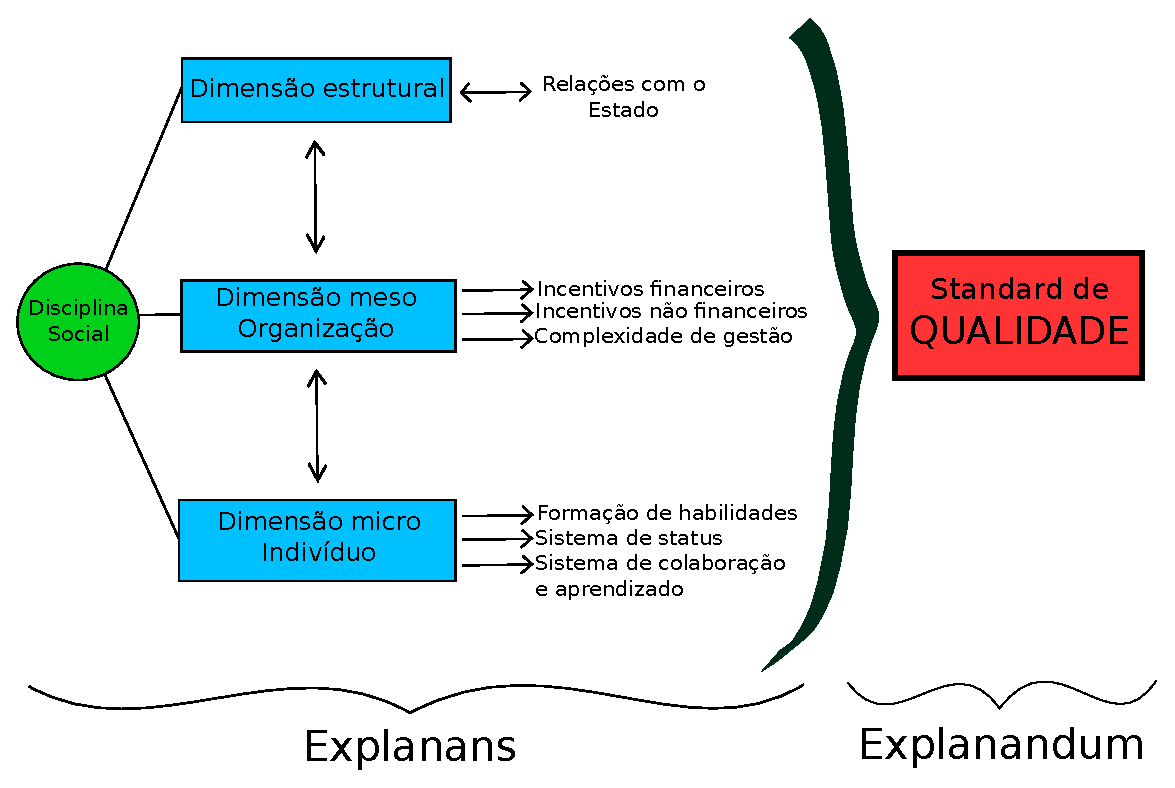
\includegraphics[scale=.8]{modelo_analise_tese.eps}
%		\fonte{Elaboração do autor.}
%	\end{figure}



	
	
	%In this research we will use a variation of the ERGM known as ``Social Selection Models''. These models were proposed by \citeonline{robins2001network} aiming to take account of the existing heterogeneity inside social structures using nodal attributes as exogenous covariables. Therefore, besides the network's own configurations, we will analyze how exogenous variables shape the emergence of the structure as well \cite{wang2016social}.
	
	\begin{comment}
	\section{Transformações de redes de 2 modos}
	
	%2-mode to 1-mode transformations allow us to investigate an affiliation network anchored in the assumption that when people are engaged in the same organizations or in the same events (a common approach in the literature), people build ties between themselves. This procedure counts one tie between two organizations when they share a person or a tie between two persons when both are engaged in the same organization \cite{brailly2016market,lazega2014redes}. The result is a 1-mode weighted network of individuals who participate in the same organizations or a 1-mode weighted network of organizations that share members.
	
	Transformações de redes de 2 modos para 1 modo nos permitem investigar uma rede de afiliações ancorada no pressuposto de que quando as pessoas estão engajadas nas mesmas organizações ou nos mesmos eventos (uma abordagem muito comum na literatura), elas constroem laços entre si. De acordo com \citeonline{denooy2011exploratory}
	
	\begin{citacao}		
		Na ciência política, economia e sociologia, muita atenção tem sido dada à composição de conselhos em grandes corporações. (\dots) Se uma pessoa é membro de um conselho de diretores em duas companhias, ele ou ela (\dots) é um diretor múltiplo que cria um diretorado conectivo ou uma conexão entre firmas. A rede de diretorados conectivos nos diz algo sobre a organização de um setor de negócios. É assumido que diretorados conectivos são canais de comunicação entre firmas\footnote{In political science, economy, and sociology, much attention has been paid to the composition of the boards of large corporations. (\dots) If a person is a member of the board of directors in two companies, he or she (\dots) is a multiple director who creates an interlocking directorate or interlock between firms. The network of interlocking directorates tells us something about the organization of a business sector. It is assumed that interlocking directorates are channels of communication between firms.}. \cite[p. 117]{denooy2011exploratory}
	\end{citacao}
	
	
	O procedimento de transformação conta um laço entre duas organizações quando elas compartilham um indivíduo afiliado ou um laço entre duas pessoas quando ambas estão engajadas na mesma organização \cite{brailly2016market,lazega2014redes}. O resultado é uma rede ponderada de 1 modo de indivíduos que participam nas mesmas organizações ou uma rede ponderada de 1 modo de organizações que compartilham membros.
	
	\end{comment}

	
	
	



	\section{Síntese teórica}

	% White - qualidade
	Neste trabalho, procuramos entender o funcionamento dos mercados de produção da música de concerto, bem como suas bases operacionais. Aqui, os mercados serão analisados como estruturas em rede \cite{white2002markets}. A disciplina em torno da qual funciona o mercado da música orquestral é uma \textit{interface} e sua ordem de valor é dada pela \textbf{qualidade} \cite{white2002markets}. A qualidade é reguladora da ação conjunta pois todos os participantes do mercado seja qual for sua natureza (indivíduos ou organizações) tiram dela suas bases normativas básicas da vida social imbuídas na estrutura. Dito de outra forma, é a partir da qualidade percebida e do \textit{Ranking} de orquestras advindo da escala de qualidade como marco regulatório (a interface do mercado) que os agentes (identidades) agem sobre a estrutura em que estão. A qualidade, entretanto, não é algo inerente às organizações mas um atributo que emerge de múltiplas interações tanto no nível das organizações quanto no nível dos indivíduos. Explicar como emerge a qualidade no mercado das orquestras configura o centro desta investigação.

	% Estado
	Para além da disciplina, o mercado da música orquestral encontra no Estado o seu segundo articulador mais importante.	De acordo com \citeonline{fligstein2002architecture}, o Estado possui um papel fundamental na regulação e, consequentemente, na estabilização dos mercados. No contexto brasileiro, a máquina estatal figura como principal financiador das orquestras mesmo que atuando de forma indireta (através das leis de incentivo à cultura). As leis de incentivo à cultura funcionam como catalisadores da produção cultural no país (quer seja a nível federal, estadual ou municipal) e fora do seu escopo há poucas produções acontecendo estando mais voltadas ao entretenimento. As únicas produções que são capazes de subsistir prescindindo desse mecanismo de financiamento são, normalmente, grandes shows ou grandes espetáculos promovidos por grandes empresas.

	% Nível da organização - incentivos financeiros e não financeiros, capacidade de gestão
	Mais ao nível da organização, é possível apontar algumas atributos que exercem influência sobre a construção de sua identidade e, consequentemente, seu posicionamento na estrutura mercantil. São eles o \textit{salário pago} e a capacidade de gestão da organização ou de sua instituição mantenedora. Suspeitamos que haja uma forte correlação entre o salário pago pelas orquestra e a percepção de seu posicionamento no \textit{Ranking} de qualidade. 
	%Do mesmo modo, as orquestras podem criar sistemas de incentivos aos músicos onde o retorno pode passar tanto pelo prestígio quanto pela realização pessoal. Uma audição interna para a escolha de um solista para um dos concertos na temporada ou uma foto de um músico estampada no encarte mensal são exemplos de incentivos não financeiros.
	Finalmente, quando nos referimos à capacidade de gestão da instituição, estamos visando sua estrutura formal. É razoável pensar que uma organização que possua uma estrutura formal mais complexa será melhor avaliada no \textit{Ranking} da qualidade do que organizações com estruturas formais mais simples. O discurso comum no campo é de que ``orquestras mais organizadas são melhores''.

	% isomorfismos
	Segundo \citeonline{dimaggio1983iron}, as organizações se engajam em processos que as levam a se tornarem cada vez mais parecidas. Esses isomorfismos acontecem como estratégia de estabilização e segurança contra as incertezas do mercado. No caso das orquestras, isso parece ser uma estratégia de diferenciação em nichos de mercado claramente perceptíveis, sobretudo no que toca ao estilo de especialidade da orquestra. Hoje, há orquestras especializadas em música antiga, em música contemporânea, em música \textit{pop}, etc.


	% coopetição
	Vimos que no exercício cotidiano de suas atividades, embora estejam em situação de competição, as organizações entram em processos supraintencionais de cooperação como estratégia que visa a estabilização do mercado, o que ficou conhecido como \textit{coopetição} \cite{lazega2009theorie}. Elas se organizam em nichos de mercado identificáveis por análise de equivalência estrutural. No mercado das orquestras esse processo pode acontecer por meio de trocas de recursos (partituras, equipamentos, ajudas financeiras propriamente dito), de informação e/ou conhecimento. Músicos que tocam em mais de uma orquestra, regentes e solistas convidados podem ser alavancas para trocas de informação e conhecimento.

	Mais ao nível do indivíduo, podemos indentificar alguns atributos que possam ter influência na qualidade atribuída a uma determinada orquestra. Esses atributos passam pelas habilidades adquiridas pelos músicos onde entram tanto o seu ambiente de formação quanto o seu professor (a construção das habilidades artísticas do músico, argumentamos, possuem tanto uma dimensão técnica relacionada à sua habilidade de tocar propriamente dita, quanto uma dimensão simbólica associada ao prestígio de seu professor e da instituição de ensino que frequentou). Além disso, no nível da interação é que podemos verificar um sistema de status entre músicos e um sistema de colaboração e aprendizado.

	Dadas essas breves definições iniciais, podemos explicitar algumas proposições centrais que nortearão a condução de nosso pensamento: (1) Os mercados de produção da música orquestral operam e encontram sua estabilização ancorados num padrão de qualidade comum com o qual todos assumem compromisso. Esse padrão de qualidade também dá origem a um ordenamento interorganizacional que reflete a interface do mercado e que é amplamente reconhecido. (2) A qualidade, o principal mecanismo articulador da estrutura, emerge do próprio mercado no fluxo das interações entre organizações e agentes. 
	% Os agentes com maior peso na emergência da qualidade são os professores e os \textit{hubs}, músicos com grande centralidade na estrutura.

        \section{Indicadores}\label{sec:geradores_nomes}
	
	%Our study object presents itself as a multilevel structure: the meso/organizational level represented by social groupings, in this case, orchestras and organizations and their relations with the State, the micro, individual level and the affiliations between the two levels \cite{brailly2016market,eloire2009reseaux,lazega2008catching,favre2016inter,lazega2016synchronization}.
	
	Nosso objeto de estudo se apresenta como uma estrutura em rede multinível: o nível organizacional representado pelos grupos sociais, neste caso, as orquestras e demais organizações com quais elas mantém relação e o Estado, o nível individual composto aqui pelos músicos da cidade de Belo Horizonte e as afiliações entre os dois níveis.
	

	%The structure in the individual level, musicians, will be tracked from advisement networks\footnote{Cf. Appendix 2 - Sociometric online questionnaire - individuals.} (aiming to capture artistic prestige), friendship networks and job indication networks. We will adopt degree centrality, betweeness centrality and constraint as indicators for finding \textit{hubs}. We will also investigate some of the individuals' \textbf{attributes} such as country of origin, the city of origin, training institution and teacher along with demographic information. This indicators show us a little of the musicians' \textbf{context} and how he can be situated \textit{a priori} in a prestige scale within the field. The name generators will be as follows:
	
	A estrutura do nível individual será investigada a partir de redes de aconselhamento\footnote{Cf. Apêndice 2 - Questionário sociométrico online - indivíduos.} (com o objetivo de capturar o prestígio individual), redes de amizade, indicação para trabalhos e convites para se apresentar conjuntamente. Adotaremos a centralidade de grau, a centralidade de intermediação e o \textit{constraint} como indicadores para encontrar os \textit{hubs}. Investigaremos também alguns dos atributos individuais como país de origem, cidade de origem, instituição de treinamento musical e professor junto com algumas variáveis sociodemográficas. Esses indicadores nos mostram um pouco do contexto dos músicos e como eles podem ser situados \textit{a priori} numa escala de prestígio dentro do campo. Os geradores de nomes aplicados foram:
	
	\begin{enumerate}
		\item Se o(a) senhor(a) precisasse de aconselhamento sobre a interpretação de alguma peça, independente do período ou do estilo da obra, a quem o(a) senhor(a) pediria conselho? Mencione quantas pessoas o(a) senhor(a) quiser.
		\item O(a) senhor(a) costuma se encontrar com outros músicos em ocasiões sociais fora do horário de trabalho? Com quem o(a) senhor(a) se encontra? Mencione quantas pessoas o(a) senhor(a) quiser.
		\item Se o(a) senhor(a) fosse indicar um músico para uma excelente posição em uma orquestra, a quem o(a) senhor(a) indicaria? Mencione quantas pessoas o(a) senhor(a) quiser independente do instrumento.
		\item Se o(a) senhor(a) fosse responsável por organizar um recital ou um concerto no qual o(a) senhor(a) fosse tocar, independente da instrumentação das obras que o senhor poderia escolher, a quem o(a) senhor(a) convidaria para tocar com o(a) senhor(a)? Mencione quantas pessoas o(a) senhor(a) quiser.
	\end{enumerate}




	
	
	%\section{Proposta de indicadores}
	
	%Com o intuito de operacionalizar o desenho de pesquisa descrito supra, buscaremos os seguintes indicadores: para verificar o padrão de qualidade vigente, verificaremos a representação dos músicos dos atributos da qualidade. Para verificar o Ranking das orquestras, utilizaremos um conjunto de indicadores: a representação dos músicos sobre o Ranking, o preço médio do ingresso, a quantidade de concertos por temporada e o volume total de investimentos. O preço médio do ingresso é adotado aqui como uma \textit{proxy} da qualidade embasado no achado de \citeonline{throsby1983quality} (a demanda é inelástica em relação ao preço mas altamente correlacionada com relação á qualidade percebida). Argumentamos que esta é uma boa proxy pois as pessoas estariam dispostas a pagar mais por um concerto que percebem como sendo de alta qualidade. A quantidade de concertos e o volume total de investimentos parecem, à primeira vista, \textit{proxys} menos seguras do que a anterior pois percebe-se um risco de cair numa tautologia. As orquestras são boas porque tem mais financiamento ou tem mais financiamento porque são boas? Tocam mais porque são boas ou são consideradas boas porque tocam mais? Contudo, argumentamos que, se adotados com parcimônia e sempre conjugados a outras variáveis, esses indicadores podem dar \textit{insights} valiosos sobre o campo. Pretendemos testar um índice de qualidade criado a partir da aglutinação dessas variáveis através de uma análise fatorial\footnote{Em linhas muito gerais, a análise fatorial é uma técnica de análise multivariada que visa reduzir a complexidade dimnuindo as dimensões a serem analisadas em índices ou escores \cite{mingoti2005analise}.}.
	
	
	%Para capturar as interações no nível individual, construiremos redes relacionais entre músicos a partir de questionários sociométricos. Maiores detalhes sobre o questionário serão apresentados na seção seguinte. Por ora é suficiente indicar que adotaremos a centralidade de grau, centralidade de intermediação e o \textit{constraint} como indicadores para encontrar os \textit{hubs}. Os atributos dos indivíduos, as variáveis exógenas às redes, serão mensuradas pelo país de origem, cidade de origem, instituição de formação e o professor. Esses indicadores nos mostram um pouco do contexto do músico e de como ele pode ser situado a priori numa escala de prestígio em meio ao campo.
	
	%A estrutura de incentivos oferecida pela orquestra será mensurada através do salário médio e dos níveis salariais dos músicos\footnote{Pretendemos comparar entre orquestras tanto a média geral do salário quanto o salário por funções específicas, e.g., spalla e chefes de naipe que comumente ganham mais do que os demais músicos de seção.}. Os incentivos não financeiros serão mensurados pela quantidade de vezes em que um membro da orquestra se apresentou como solista ou teve um concerto de câmara agendado em nome da orquestra\footnote{É comum às orquestras organizarem concertos com formações menores como quartetos de cordas ou quintetos de metais com músicos selecionados entre seus membros.}. A complexidade da gestão será mensurada pela quantidade de setores e diretorias que a orquestra/instituição mantenedora possui e pela quantidade de níveis hierárquicos do instrumentista até o presidente.
	
	%Os indicadores escolhidos para mensurar o nível de interação com o Estado são o volume financeiro investido pelo próprio Estado e a existência/quantidade de contratos, convênios ou parcerias firmados.
	
	
	
	%The upper level is composed by the orchestras and all the other organizations with whom they maintain any kind of relation, whether it is an economic relation, a partnership or a resources exchange agreement\footnote{Cf. Appendix 3 - Sociometric questionnaire - organizations.}. We will track the organizations' main activity, it's style (in White's terms), it's formal structure and it's collaboration ties. The \textbf{incentive structure} offered by the orchestra will be measured through average salary and salaries of musicians\footnote{We intend to compare both the average salary and specific salary by function, e.g., concertmaster and other leaders inside the orchestra that commonly earn more money than the other section musicians.}. The \textbf{non-financial incentives} will be measured by the number of times an orchestra member played as a soloist or in a chamber music concert in the orchestras' season\footnote{It is common to professional orchestras to organize concerts with smaller ensembles as string quartets or brass quintets with selected musicians.}. The \textbf{management complexity} will be measured by the quantity of sections and boards that the orchestra/maintainer have and by the amount of hierarchical levels between the instrumentalist and the CEO.
	
	O nível organizacional é composto pelas orquestras e todas as outras organizações com as quais elas mantêm algum tipo de relação, seja uma relação econômica, uma parceria ou uma troca de recursos\footnote{Cf. Apêndice 3 - Questionário Sociométrico - organizações.}. Investigaremos a principal atividade das organizações, seu estilo (nos termos de White), sua estrutura formal e seus laços. 
	%Os incentivos não financeiros serão investigados pela quantidade relativa de vezes que os membros da orquestra se apresentaram como solistas ou em concertos de câmara durante a temporada\footnote{É comum as orquestras profissionais organizarem concertos com grupos menores como quartetos de cordas ou quintetos de metais com músicos selecionados.}. 
	A complexidade organizacional será mensurada pela quantidade de setores ou diretorias que a orquestra possui, pelo número de níveis hierárquicos que separam os músicos do CEO e pelo seu orçamento anual. A proximidade com o Estado será mensurada a partir do volume financeiro investido diretamente pelo Estado nas organizações e, quando não for o caso, a quantidade de projetos financiados pela iniciativa privada via Leis de Incentivo à Cultura.
	
	
	%Table \ref{indicadores-relational} show a synthesized version of the proposed indicators regarding the relational data and the organizational level.
	
	A Tabela \ref{indicadores-relational} mostra uma versão sintetizada dos indicadores propostos relacionados aos dados relacionais nos níveis individual e organizacional.
	
	%Os indicadores aqui elencados estão apresentados de forma resumida na Tabela \ref{indicadores}. Seguimos apresentando os dados a serem coletados e os métodos de análise utilizados.
	
	
	\begin{table}[!ht]
		\ibgetab{
			\centering
			\caption{Indicadores propostos - dados relacionais}
			\label{indicadores-relational}
		}
		{\begin{tabular}{|c|c|}
				
				\hline
				\textbf{Conceito - Nível individual} & \textbf{Indicador} \\
				\hline
				Interação individual & Redes \\
				\hline
				Atributos individuais de interesse & País de origem  \\
				& Cidade de origem  \\
				& Insituição de formação \\
				& Professor    \\
				\hline
				Informações demográficas & Idade \\
				& Sexo \\
				& Renda total \\
				& Escolaridade \\
				& Cor da pele \\
				& Estado civil \\
				& Número de filhos \\
				\hline
				\textbf{Conceito - Nível organizacional} & \textbf{Indicador} \\
				\hline
				Interação organizacional & Redes \\
				\hline
				
				Complexidade Organizacional  & Número de setores/diretorias  \\
				& Distância em níveis entre os músicos e o CEO \\
				& Orçamento anual \\
				\hline
				Proximidade com o Estado & Financiamento total do Estado \\
				& Quantidade de projetos incentivados \\
				\hline
				Salário pago & Salário médio pago aos músicos \\
				\hline
				
			\end{tabular}
		}
		{\fonte{Elaborado pelo autor.}}
	\end{table}
	


	Apresentaremos agora nossas principais hipóteses de trabalho.
	
	\section{Hipóteses}\label{hipoteses}
	
	\newtheorem{hip}{Hipótese}

	%We depart from the central assumption that the quality standard, the gravity center of orchestras' market, emerges from its own structure. At the individual level, we argue that the concepts of a ``good orchestra'', a ``good performance'', a ``good instrumental technique'', emerge from the bottom up and not from top down. Also, that seems to be a struggle for the ``right'' to the definition of quality. This leads us to hypotheses regarding individuals, organizations and their relation with the State.
	
	Partimos do pressuposto central de que o padrão de qualidade, o centro gravitacional do mercado das orquestras, emerge de sua própria estrutura. No nível individual, argumentamos que os conceitos de ``boa orquestra'', ``boa performance'', ``boa técnica instrumental'', emergem de baixo para cima e são fortemente influenciados pelos atores de maior prestígio na rede. Além disso, parece haver uma disputa pela ``correta'' definição da qualidade tanto entre músicos quanto entre dirigentes de orquestras. Traçamos, portanto, as seguintes hipóteses:

        Tomando a qualidade percebida de uma orquestra como a qualidade percebida dessa organização entre os músicos que compõem a estrutura do mercado, postulamos que 
	

        \begin{hip}\label{hip:redecomplexa}
		%The more complex an orchestra's business network, the better it will be positioned in quality ranking.
		Quanto mais complexa a rede de negócios de uma orquestra (em termos de tamanho e densidade), melhor será sua qualidade percebida.
	\end{hip}

        Considerando que o músico é o principal ``insumo'' da orquestra na construção de seu produto final, o concerto, postulamos que
        
	\begin{hip}\label{hip:musprest}
		Quanto maior for a concentração de músicos prestigiosos numa orquestra, melhor será sua qualidade percebida.
	\end{hip}
	

	
	\begin{hip}\label{hip:incentivos}
		%The more an orchestra provides structural incentives for the musicians, the better it will be positioned in quality ranking.
		Quanto melhor for a média salarial de uma orquestra para seus músicos, melhor será sua qualidade percebida.
              \end{hip}

              No que toca à hipótese apresentada acima, é importante salientar que no caso brasileiro os músicos de seção (músicos que não possuem funções de chefia de naipe e que necessariamente estão num ponto acima na hierarquia orquestral) possuem, normalmente, o mesmo salário. O pagamento não se diferencia pela experiência ou prestígio dos músicos. A média do salário pago se apresenta, portanto, como um indicador do investimento da organização em seus músicos.
              
	
	\begin{hip}\label{hip:orcamento}
		Quanto maior for o orçamento anual de uma orquestra, melhor será sua qualidade percebida.
	\end{hip}
	
	% Quanto mais incentivos as orquestras proporcionam a seus músicos, mais elas tendem a ocupar as primeiras posições no Ranking de qualidade.


        Tomando a complexidade da estrutura organizacional como um indicador para capacidade administrativa, 
        
	\begin{hip}\label{hip:estruturacomplexa}
		%The more complex the organizational structure of an orchestra or of its maintainer, the better it will be positioned in quality ranking.
		Quanto mais complexa for a estrutura organizacional de uma orquestra ou de sua mantenedora, melhor será sua qualidade percebida.
              \end{hip}

              Nesse caso, estamos considerando complexidade de estrutura organizacional como a quantidade de setores ou diretorias da orquestra (ou de sua mantenedora) bem como a distância - em departamentos - entre o músico e a presidência.
	
	
	%Por fim, num nível macro, o nível do próprio mercado e sua relação com o Estado, argumentamos que
	Por fim, tomando em conta o protagonismo do Estado na promoção e no fomento das atividades culturais no contexto brasileiro, postulamos que
	
	\begin{hip}\label{hip:proxestado}
		%The closest the relationship of an orchestra with the State, the better it will be positioned in quality ranking.
		Quanto mais próximas as relações de uma orquestra com o Estado, melhor será sua qualidade percebida.
	\end{hip}


        Estas são as hipóteses que nos interessam testar neste trabalho. Maiores detalhes sobre a operacionalização dos testes das hipóteses serão apresentados no capítulo a seguir.






	\begin{comment}





	%\subsection{A perspectiva da sociologia econômica}

	\ldots













	\citeonline{white1993canvases} conduziram um estudo sobre a mudança técnica e sobre as carreiras dos pintores franceses do séc. XIX dando origem à chamada escola ``impressionista''. Para esses autores,



	\begin{citacao}

		A arte não é um tipo de brinquedo manipulado em seu desenvolvimento por forças sociais e econômicas. Mesmo assim, pintores mostram grande interesse em como se tornarem reconhecidos e viver de sua arte. Os padrões e relações no trabalho desses indivíduos tornam-se possíveis e são controladas por pressões institucionais das quais nenhum homem está apercebido. Os quadros e carreiras dos indivíduos mudam e são mudados pelas instituições peculiares ao mundo da arte\footnote{Art is not a kind of tinkertoy manipulated in its development by social and economic forces. Yet, individual painters do show deep interest in how to become recognized and make a living. The patterns and relations in the work of these individuals are made possible and are constrained by institutional pressures of which no one man is quite aware. The canvases and careers of individuals change and are changed by the institutions peculiar to the art world.}. \cite[p. xxi]{white1993canvases}

	\end{citacao}



	Esses autores entendem o sistema institucional como uma ``rede persistente de crenças, costumes e procedimentos formais que juntos formam uma organização social mais ou menos articulada com um objetivo central conhecido – aqui a criação e reconhecimento da arte\footnote{(…)a persistent network of beliefs, customs, and formal procedures which together form a more-or-less articulated social organization whit an acknowledged central purpose – here the creation and recognition of art.}'' \cite[p. 2]{white1993canvases}.



	Pierre Bourdieu tem também uma contribuição significativa nessa área de estudos. O autor desenvolveu o conceito de ``campo'' para estudar diversas ramificações do mundo econômico: o mercado imobiliário \cite{bourdieu2005social}, o campo científico \cite{bourdieu2008ciencia}, e o campo literário \cite{bourdieu2005regras} para citar alguns exemplos. Para Bourdieu



	\begin{citacao}

		Quando falamos de um \textit{campo} de tomadas-de-posição, estamos insistindo que o que pode ser constituído como um \textit{sistema} pelo bem da análise não é o produto de uma intenção de buscar coerência ou um consenso objetivo (mesmo se isso pressupõe concordância inconsciente ou princípios comuns) mas o produto e prêmio de um conflito permanente; ou, para colocar de outra forma, que o princípio gerativo, unificador desse 'sistema' é a luta, com todas as contradições que ele engendra\footnote{When we speak of a \textit{field} of position-takings, we are insisting that what can be constituted as a \textit{system} for the sake of analysis is not the product of a coherence-seeking intention or an objective consensus (even if it presupposes unconscious agreement of common principles) but the product and prize of a permanent conflict; or, to put it another way, that the generative, unifying principle of this 'system' is the struggle, whit all the contradictions it engenders.}. \cite[p. 34]{bourdieu1993field}

	\end{citacao}



	Num estudo sobre compositores de trilha sonora na indústria cinematográfica de Hollywood, \citeonline{faulkner2003music} busca entender de que forma compositores se associam a produtores de cinema dando origem às redes de produção hollywoodianas, quais são os compositores mais centrais no sistema e quais deles, por conseguinte, tem domínio sobre a rede. Para isso, além de uma grande pesquisa etnográfica, o autor monta uma matriz de afiliação indicando quais compositores trabalharam com quais produtores e, com uso de um \textit{blockmodeling}, separa ambos os profissionais em quatro subgrupos onde os membros de um mesmo grupo são estruturalmente equivalentes. Para dividir os compositores em um mesmo subgrupo o critério usado pelo autor foi de consistência, não conectividade. Por exemplo:



	\begin{citacao}

		Fred Karlin e Michael Small são figuras grandes e centrais em Hollywood. Eles compuseram para filmes de um mesmo produtor ao longo dos doze anos. Os pontos de trabalho em suas linhas de carreira convergem. Na medida em que eles ``compartilham'' subgrupos de cineastas, são mais propensos a aparecer juntos na matriz da Grande Hollywood. Os compositores Karlin e Small trabalharam para o produtor e diretor Alan J. Pakula, cujos créditos incluem \textit{The sterile Cuckoo} (1969), \textit{Klute} (1971), \textit{The Parallax View} (1974), \textit{All the President's Men }(1976), e antes, \textit{Up the Down Staircase }(1967), \textit{The Stalking Moon }(1968), e \textit{Love with the Proper Stranger }(1963). Se o compositor David Shire se junta a Karlin e Small, como fez quando compôs a trilha para o sucesso \textit{All the President's Men}, ele é mais propenso a mostrar um padrão de equivalência em suas conexões a essa parte do mercado, a parte ou nicho feita pelos filmes de Alan Pakula e suas seleções de compositores para esses filmes.



		Similarmente, quando John Williams é contratado pelo cineasta Walter Mirisch, e Jerry Fielding e John Mandel são também contratados por Mirisch, há um padrão de conexões comuns entre os três a este, um cineasta altamente produtivo. Todos os três estão consistentemente ligados a um empregador comum. Todos os três foram sujeitos ao controle de Mirisch como empregador e como um ``cliente'' para seus serviços.



		De acordo com que ``sets'' múltiplos de produtores de filme, como Pakula e Mirisch, contratam os serviços de freelancers como Shire, Karlin, Williams, Fielding, Mandel e Small, um padrão de equivalência começa a emergir. \cite[p. 186]{faulkner2003music}

	\end{citacao}



	Com essa análise, Faulkner consegue identificar quais são os compositores que tem o mesmo padrão de conexões com produtores. Adicionando a essa informação medidas de produtividade (quais deles tem o maior número de créditos) e de reconhecimento (quais deles tem indicações e vitórias no Oscar, quais filmes cujas trilhas foram compostas por eles foram indicados e ganharam o Oscar), o autor identifica quais são os principais compositores do mercado de filmes em Hollywood, aqueles que tem o controle do sistema.



	Seguiremos a linha de análise desenvolvida por \citeonline{white1993canvases} e \citeonline{becker2008art} no que tange os processos de produção e distribuição pelo fato de esses autores, como já dito, entenderem o sistema de produção da arte como redes de cooperação.



	\end{comment}



	\begin{comment}





	%\subsection{O Mercado dos Concertos}



	Compreender o mercado da música de concerto exige entendimento acerca das convenções vigentes, dos recursos que são mobilizados no processo de cooperação entre atores e como esses recursos circulam na rede, da distribuição/comunicação das instituições artísticas envolvidas, do papel dos críticos na formação de opiniões, do papel do Estado como regulador e principal financiador, dos processos de mudança no mundo da música de concerto e da construção da reputação dos atores envolvidos. Discorreremos brevemente acerca desses pontos. Características relevantes do público frequentador e sua influência no consumo dos concertos serão abordadas oportunamente.



	Para \citeonline{becker2008art} as convenções exercem grande controle sobre os artistas em virtude de sua complexidade sistêmica; para que alguma convenção sofra mudança, uma diversidade de outras mudanças é necessária. ``Um sistema de convenções toma corpo em equipamentos, materiais, treinamento, espaços e lugares disponíveis, sistemas de notação, e similares, os quais devem ser mudados se qualquer componente é mudado \footnote{A system of conventions gets embodied in equipment, materials, training, available facilities and sites, systems of notation, and the like, all of which must be changed if any one component is.}'' \cite[p.32]{becker2008art}. Se um compositor escreve uma música num sistema de 42 microtons dentro de uma oitava ao invés do sistema habitual de doze semitons, surge a necessidade da construção de instrumentos específicos para que essa música seja tocada. Os instrumentos ocidentais em sua grande maioria não são capazes de produzir intervalos menores do que um semitom (algumas exceções seriam os instrumentos da família das cordas pelo fato de não serem temperados\footnote{Em outra oportunidade, estudamos de que modo o processo chamado de temperamento dos intervalos da série harmônica e a consequente forma de construção dos instrumentos ocidentais modernos dão corpo ao processo de racionalização da música ocidental \cite{weber1995fundamentos}}). Algumas obras de Villa-Lobos, para citar outro exemplo, fazem uso de instrumentos de percussão nunca antes utilizados e inspirados em instrumentos dos índios da Amazônia. Quando da apresentação dessas obras, os percussionistas da orquestra precisam construir os instrumentos a partir de orientações deixadas por Villa-Lobos.



	Além dos recursos financeiros necessários, uma longa lista pode ser feita abarcando recursos materiais e recursos humanos (\textit{personnel}). \citeonline{becker2008art} comenta a respeito do controle que os artistas podem sofrer em seu processo criativo no caso de um alto nível de especialização técnica ou monopolização de recursos dos colaboradores:



	\begin{citacao}

		Eles [os artistas] escolhem do conjunto do que está disponível para eles no mundo da arte em que trabalham. Os mundos diferem em o que eles tornam disponível e na forma pela qual tornam-no disponível. Os padrões de atividade econômica característicos de uma sociedade moldam com o que os artistas podem trabalhar e com quem eles podem trabalhar. Fatos como o grau de monopolização da produção de materiais, a rentabilidade de mercados menores e o grau no qual os artistas precisam de itens especialmente desenhados e manufaturados para eles afeta o que está disponível e, portanto, o que os artistas podem fazer. Similarmente, as organizações pelas quais o pessoal de suporte encontra os projetos nos quais trabalham criam motivos organizacionais, profissionais e de carreira que podem ir de encontro às intenções dos artistas que os empregam \footnote{They choose these out of the pool of what is available to them in the art world they work in. Worlds differ in what they make available and in the form in which they make it available. The patterns of economic activity characteristic of a society shape what artists can get to work with and who they can get to work with them. Such facts as the degree of monopolization of production materials, the profitability of minority markets, and the degree to which artists need items specially designed and manufactured for them all affect what is available and thus what artists can do. Similarly, the organizations through which support personnel find the projects they work on create organizational, professional, and career motives which may run counter to the intentions of the artists who employ them.}. \cite[p. 92]{becker2008art}

	\end{citacao}



	Há um papel essencial representado pelos \textit{dealers}, os produtores ou os agentes, no caso das estrelas da música de concerto, na circulação de recursos e financiamento. No contexto brasileiro onde a grande maioria dos concertos são realizados através de incentivos fiscais do Estado às empresas patrocinadoras, esses \textit{dealers} são os intermediários entre os artistas e o dinheiro. As empresas que investem em séries de concertos geralmente escolhem os projetos nos quais investirão visando maior retorno simbólico para sua marca. Esta forma de alocar os recursos disponíveis será discutida oportunamente.



	Os críticos e os ``esteticistas'' (\textit{aestheticians}) são responsáveis por definir o que é e o que não é boa música de concerto, o que é e o que não é uma boa apresentação e tem um papel fundamental no sistema de produção da música de concerto. Nos estudos de socioeconomia franceses, estes são os prescritores da boa qualidade. Os sistemas estéticos e de classificação construídos por eles produzem reputação. ``Distribuidores e membros do público levam em conta as reputações quando decidem o que apoiar emocionalmente e financeiramente, e isso afeta os recursos disponíveis aos artistas para continuar seu trabalho\footnote{Distributors and audience members take reputation into account when they decide what to support emotionally and financially, and that affects the resources available to artists to continue their work.}'' \cite[p. 131]{becker2008art}.



	No Brasil, praticamente todos os concertos de orquestras são feitos mediante alguma ``lei de incentivo à cultura''. Essas leis operam em um mecanismo de incentivo fiscal aonde as empresas podem escolher alguns projetos culturais para investir parte dos impostos devidos. Desse modo, o caminho entre o recurso público e o artista é encurtado já que o Estado prescinde do recolhimento do imposto e possibilita a alocação do recurso diretamente ao projeto no mercado. Curioso notarmos que, embora o recurso provenha do Estado, o poder de alocação dele está nas mãos das empresas. Isso gera uma série de controles aos artistas e dá mais poder aos \textit{dealers} e captadores mencionados supra. Interessa-nos pesquisar de que forma esse mecanismo, que parece ser a principal forma de financiamento no país, exerce controle sobre as orquestras. Entretanto, os agentes públicos podem atuar contribuindo para a autonomia do artista como comenta Becker:



	\begin{citacao}

		A despeito dos controles, alguns governos tem sido responsáveis por trabalhos contemporâneos de grande porte. Em tais casos, oficiais especializados, ``iluminados'' no sentido de Haskell [patrocinadores com recursos suficientes e conhecimento necessário para entender as obras], compartilhando as convenções e estética de artistas no mundo da pintura e escultura contemporâneas, tomam o controle o trabalho diário de burocracias que administram fundos apropriados para arte. Eles isolam artistas de alguma, embora não toda, pressão política direta. André Malraux, enquanto era ministro da cultura no governo francês, exemplifica o tipo\footnote{Despite these constraints, many governments have been responsible for major contemporary works. In such cases, specialized officials, ``enlightened'' in Haskell’s sense, sharing the conventions and aesthetic of artists in the contemporary painting and sculpture world, take over the day-to-day workings of the bureaucracies which administer funds appropriated for art. They insulate artists from some, though not all, direct political pressure. André Malraux, while he was minister of culture in the French government, exemplifies the type.}. \cite[p. 105]{becker2008art}

	\end{citacao}



	Para Becker, os mundos da arte estão em constante mudança. Os processos e modos de produção, com o passar do tempo vão se transformando mesmo porque, na visão do autor, ninguém faz algo duas vezes exatamente da mesma maneira \cite[p. 301]{becker2008art}. Convenções, recursos materiais, modos de produção e distribuição quando mudam podem ou não impor novos aprendizados às pessoas envolvidas no sistema. Quando não impõem novos aprendizados são chamados de \textit{drifts}. Quando impõem, são chamados pelo autor de ``revoluções'' evocando a Thomas Kuhn.



	\begin{citacao}

		Revoluções artísticas fazem grandes mudanças no caráter das obras produzidas e nas convenções usadas para produzi-las. Assim, os impressionistas e cubistas mudaram a linguagem visual existente, o modo como se põe tinta na tela de modo que seja lido como uma representação de algo. Schoenberg, Berg e Webern fundamentalmente mudaram a lógica das relações entre notas musicais quando introduziram o sistema dodecafônico na composição \footnote{\textbf{FALTA TRADUÇÃO DESTE TRECHO}}.\cite[p. 305]{becker2008art}

	\end{citacao}



	Dois exemplos de revoluções puderam ser observados nos últimos anos. A primeira relacionada ao modo de distribuição da música: com o crescimento da pirataria e da utilização dos arquivos MP3's, a venda de discos diminuiu significativamente levando algumas empresas a sérias crises financeiras, apesar de não infligir nenhuma mudança no caráter das músicas. Algum tempo depois, começaram a surgir os primeiros discos digitais, músicas em formato MP3's que eram comercializadas online. Além de comprar o disco inteiro, o consumidor tinha ainda a opção de comprar apenas uma ou quantas músicas quisesse. A segunda, explorando possibilidades expressivas da área, foi observada em uma montagem da ópera ``O Barbeiro de Sevilha'' pela Cia. Brasileira de Ópera apresentada em todo o Brasil no ano de 2010. A ópera foi encenada usando recursos de projeção digitais de modo que os cantores contracenavam com personagens em desenho animado (FIG. 1)



	\begin{figure}[h]

		\centering

		\caption{O Barbeiro de Sevilha. Cia Brasileira de Ópera.}

		%\includegraphics{imagefile}

		\legend{FONTE: \ldots}

	\end{figure}



	Finalmente, ao abordar de que modo a reputação de um artista é construída, Becker mostra que, se o foco da análise de um pesquisador ou crítico de arte está no artista como indivíduo, faz sentido evocar uma teoria da reputação que está assentada sobre cinco pressupostos.



	\begin{citacao}

		(1) Pessoas especialmente dotadas (2) criam obras de excepcional beleza e profundidade que (3) expressam emoções humanas profundas e valores culturais. (4) As qualidades especiais da obra testificam dos dons especiais de seu autor, e esses dons do autor já conhecidos testificam das qualidades especiais da obra. (5) Desde que a obra revela as qualidades essenciais e o valor do autor, todas as obras que essa pessoa fizer, mas não outras, deveriam ser incluídas no corpus sobre o qual sua reputação está baseada \footnote{(1) Specially gifted people (2) create works of exceptional beauty and depth which (3) express profound human emotions and cultural values. (4) The work’s special qualities testify to its maker’s special gifts, and the already known gifts of the maker testify to the special qualities of the work. (5) Since the works reveal the maker’s essential qualities and worth, all the works that person makes, but no others, should be included in the corpus on which his reputation is based.}. \cite[p. 352-3]{becker2008art}

	\end{citacao}



	Entretanto, o autor afirma que qualquer que seja o nível de reputação desfrutada pelo artista, esta só é possível através de um processo social de desenvolvimento que passa pela construção de um consenso perceptivo e de julgamento entre os atores que fazem parte do mundo da arte em questão, sejam eles público, críticos, artistas ou outros. Tudo o que contribui para a existência da obra de arte acaba por contribuir também para a construção de sua reputação.



	\end{comment}







	\chapter{Dados e Métodos}
	
	Os dados deste trabalho foram coletados entre os meses de setembro e dezembro de 2018. Para compreender o nível organizacional, dirigentes das orquestras foram contactados e convidados a realizar uma entrevista semiestruturada abordando questões pertinentes para a investigação. O roteiro de entrevista com os dirigentes das orquestras encontra-se no anexo 3 deste trabalho.
	
	Quanto ao nível individual, os músicos participantes das orquestras em Belo Horizonte foram contactados pessoalmente, via redes sociais e telefone, e foram convidados a responderem o questionário sociométrico apresentado no anexo 2 deste trabalho. Alguns questionários foram respondidos por telefone, outros foram respondidos numa versão online.
	
	Neste ponto, é importante salientar ao leitor que houve grande dificuldade no contato com os músicos. Atribuímos esse fator a duas razões, a saber, a carga enorme de trabalho que os músicos da cidade possuem tanto de ensaios nas orquestras quanto de estudos fora de seu horário regular de trabalho (especialmente em se tratando de repertório cuja execução é tecnicamente mais desafiadora) e ao perfil característico dos músicos que, no contexto investigado, tendem a possuir alto status sócio-ocupacional e, em geral, selecionam de forma bastante criteriosa os compromissos nos quais irão se engajar.
	
	As análises serão realizadas em duas partes. No primeira, apresentaremos uma descrição detalhada do campo a partir das entrevistas semiestruturadas realizadas com os dirigentes das orquestras. Na segunda, apresentaremos os resultados das análises para as redes observadas entre indivíduos e para as redes de indivíduos e organizações obtidas através da transformação \textit{2-mode} para \textit{1-mode} (redes de afiliações). As análises de redes se darão em 3 momentos; o primeiro consiste uma apresentação descritiva da rede com métricas básicas ao nível da rede (densidade, diâmetro, distância média e grau médio) e ao nível do indivíduo (centralidade de grau, centralidade de intermediação, centralidade de proximidade e \textit{constraint}). O segundo consiste de uma modelagem de blocos visando identificar padrões de vértices estruturalmente equivalentes. O terceiro consistirá de uma estimação de ERGM's para explicar os processos sociais que exercem influência na emergência da estrutura. Para os fins deste trabalho, utilizaremos uma variação dos ERGM's conhecida como ``Modelos de Seleção Social'' (\textit{Social Selection Model}). Esses modelos foram propostos por \citeonline{robins2001network} com o objetivo de dar conta da heterogeneidade existente dentro das estruturas sociais usando atributos dos nós como covariáveis exógenas. Desse modo, além das configurações internas da própria rede, analisaremos ainda como variáveis exógenas moldam a emergência da estrutura \cite{wang2016social}.

	Por fim, as hipóteses deste trabalho serão predominantemente testadas utilizando o \textit{Network Autocorrelation Model} (NAM). 

	%A seção dedicada à Orquestra Filarmônica de Minas Gerais será um pouco maior do que as demais unicamente porque além das entrevistas realizadas com o dirigente contatado, utilizamos como fonte também os relatórios gerenciais disponibilizados pela organização em seu site oficial.


        \chapter{Apresentação dos dados}
        
	\section{A qualidade para os músicos}
	
	Parte importante deste trabalho se deu a compreender, para além da categorização que os músicos normalmente fazem do ranking qualitativo das orquestras em Belo Horizonte, como esses músicos representam a qualidade, como eles a qualificam, como a definem. Esta questão não é de nenhum modo trivial se verificamos que existe uma grande parte da tradição sociológica que investiga como as definições da vida não são dadas mas construídas socialmente e refletem, sobretudo, as relações hierárquicas na estrutura relacional entre as pessoas. O que é ou não é uma boa orquestra, afinal, não é algo dado, mas uma definição sujeita a disputa. 
	
	No questionário online os músicos foram solicitados a explicar porque a orquestra que consideravam como a de melhor qualidade era de fato assim. A Figura \ref{wordcloud} mostra uma síntese das palavras mais faladas.
	
	\begin{figure}[!ht]
		\centering
		\caption{Nuvem de palavras - palavras mais faladas sobre a qualidade}
		\label{wordcloud}
		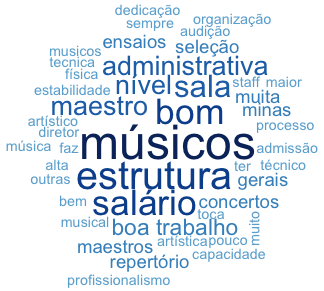
\includegraphics[scale=.8]{qualidade_wordcloud.png}
		\fonte{Elaboração do autor.}
	\end{figure}
	
	As respostas tenderam a polarizar em três grupos principais identificados a partir de uma análise de \textit{clusters} (Figura \ref{cluster}). O primeiro deles está relacionado à estrutura da orquestra e ao salário dos músicos. A maioria dos entrevistados salientou o quanto um bom salário para os músicos e uma estrutura de trabalho organizada proporciona aos músicos condições para se dedicar ao estudo técnico e do repertório selecionado. Nesse grupo estão também vários considerações à importância do maestro na condução da orquestra a uma qualidade diferenciada. Outro grupo está relacionado à qualidade técnica dos músicos bem como a um regime de contratação que não provê estabilidade, ``o que faz com que cada membro da orquestra mantenha-se sempre em forma nas suas funções'' (\textit{músico entrevistado}). Um terceiro grupo aborda o tipo de seleção realizada na orquestra e os métodos de admissão que garantem a entrada de gente comprometida com um alto nível de qualidade.
	
	\begin{figure}[!ht]
		\centering
		\caption{\textit{Cluster Analysis} - palavras mais faladas sobre a qualidade}
		\label{cluster}
		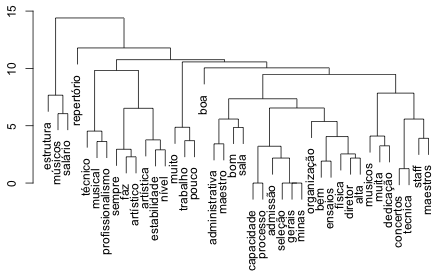
\includegraphics[scale=.8]{qualidade_cluster.png}
		\fonte{Elaboração do autor.}
	\end{figure}
	
	Embora não apareçam no dendograma apresentado na Figura \ref{cluster}, há alguns músicos que argumentam numa linha contrária à apresentada acima. Segundo esses músicos, a principal razão de considerar alguma orquestra como sendo de boa qualidade está relacionada à sua tradição, sua experiência e sua flexibilidade em transitar por diversos tipos de repertório, diversas épocas, até mesmo incluindo a música popular.
	
	Interessante notar que o fato de uma orquestra trabalhar com música popular é considerado um ``tabu'' por uma grande parcela de músicos\footnote{Aqui é importante relatar ao leitor que o autor deste trabalho possui formação acadêmica em regência e uma experiência de mais de 10 anos entre os músicos e as orquestras na cidade de Belo Horizonte. A perspectiva aqui relatada vem de um conhecimento de campo construído no decorrer da experiência profissional.}. Há um grupo que considera a prática da música popular como um comportamento desviante, que deve ser evitado a todo custo para que não atrapalhe a busca do refinamento necessário à performance da música erudita. Por outro lado, há outro grupo que acredita que a mescla de estilos é salutar e provê ao músico de orquestra habilidades técnicas e musicais às quais ele não poderia desenvolver senão com a prática da música popular, por exemplo, a improvisação, o desenvolvimento de sonoridades alternativas e inovadoras nos instrumentos. Não há um consenso a esse respeito.
	
	Os músicos que também atuam como professores responderam no questionário online a seguinte pergunta: ``Caso o(a) senhor(a) seja também professor(a), como o(a) senhor(a) faz seus alunos entenderem o que é necessário para uma boa performance?'' Essas respostas abordaram basicamente duas coisas: (1) o estudo técnico firme e concentrado realizado de maneira metódica e com muita dedicação e (2) a busca do aprimoramento da percepção musical/artística através de experiências com outros músicos, outros professores, audições, etc. Apenas um entrevistado mencionou atenção ao mercado de trabalho para que o aluno se mantenha competitivo. Entretanto, esse parece ser um comentário tangencial embora abarque, implicitamente, o argumento dominante do refinamento técnico.
	
	
	Voltemos nossa atenção agora às orquestras da cidade de Belo Horizonte. No momento da redação deste trabalho, existem cinco orquestras profissionais\footnote{A Orquestra Sinfônica da Polícia Militar não foi aqui incluída pois foge ao escopo do nosso trabalho.} de tamanhos variados atuando na cidade, a saber, a Orquestra Filarmônica de Minas Gerais\footnote{\url{http://www.filarmonica.art.br}}, a Orquestra Sinfônica de Minas Gerais\footnote{\url{http://www.fcs.mg.gov.br/index.php?option=com_gmg&view=page&id=2631&controller=page&Itemid=1281}}, a Orquestra de Câmara Sesiminas\footnote{\url{http://www7.fiemg.com.br/sesi/centro-de-cultura/belo-horizonte/produtos/detalhe/orquestra-de-camara-sesiminas}}, a Orquestra Ouro Preto\footnote{\url{http://www.orquestraouropreto.com.br}} e a Orquestra Opus\footnote{\url{https://www.facebook.com/OrquestraOpus/}}.


	\section{Orquestra Filarmônica de Minas Gerais}\label{cap:filarmonica}

	

	Criada muito recentemente, em 2008, a Orquestra Filarmônica de MG tem sido aclamada pela crítica nacional pela qualidade técnica e artística de suas apresentações. A organização pode ser divida em dois grandes setores: a orquestra propriamente dita e sua instituição mantenedora, o Instituto Cultural Filarmônica. A orquestra é composta por cerca de noventa músicos, o maestro e seu assistente, um gerente, um inspetor, um assistente administrativo, quatro arquivistas e seis montadores. Já o Instituto Cultural Filarmônica é formado pela Assembleia de Associados, pelo seu Conselho Administrativo, pela Diretoria Executiva, Equipe Técnica e Equipe Administrativa.



	A Diretoria Executiva do Instituto é formada pelo Diretor Presidente, pelo Diretor Administrativo-financeiro, pela Diretora de Comunicação, pela Diretora de MKT e Projetos, pelo Diretor de Operações e pelo Diretor de Produção Musical. A equipe técnica é formada pelo Gerente de Comunicação, Gerente de Produção Musical, Assessor de Programação Musical, Produtores, Analistas de Comunicação, Analista de MKT de Relacionamento, Analistas de MKT e Projetos, Assistente de MKT de Relacionamento, Assistente de Procução e quatro profissionais alocados na Sala Minas Gerais (Gerente de Infraestrutura, Gerente de Operações, Assistente Operacional e Técnico de Iluminação e Áudio). A equipe administrativa é formada pelo Gerente Administrativo-financeiro, Gerente de Recursos Humanos, Analistas Administrativos, Analista Contábil, Secretária Executiva, Assistente Administrativa, Assistente de Recursos Humanos, Recepcionista, Auxiliar Administrativo, Auxiliares de Serviços Gerais, Mensageiros e um menor aprendiz.



	%\begin{figure}[h]

	%	\centering

	%	\caption{Organograma da Orquestra Filarmônica de MG e do Instituto Cultural Filarmônica}

		%\includegraphics[keyvals]{imagefile}

	%	\fonte{Elaboração do autor a partir de dados disponíveis online}

	%\end{figure}



	Em seu funcionamento, ambos os setores se envolvem em relações comerciais ou artísticas com outros atores. No caso da orquestra, é comum a visita de solistas e maestros convidados. No caso do Instituto, uma rede de fornecedores nos mostra o âmbito dos recursos necessários à mobilização. Dentre os fornecedores do Instituto há assessoria contábil, assessoria jurídica, assessoria de imprensa, assessoria em TI, \textit{clipping}, criação e finalização de som, fotógrafos, gestão de projetos culturais, gráfica rápida, impressão digital, produção audiovisual, produção gráfica, sistema de assinaturas e compra de ingressos, serviços de segurança eletrônica, sistema de gestão e a redação de notas para os programas dos concertos.

	
	Na lógica estrutural da orquestra Filarmônica, cada diretoria possui técnicos ligados a sua atividade fim logo abaixo do diretor. Ainda logo abaixo do diretor há um gerente, abaixo deste há um analista ao que se seguem os assistentes e os auxiliares. É possível entender a estrutura da diretoria artística, diretoria onde os músicos estão inseridos, a partir da mesma estrutura. De acordo com o dirigente entrevistado, a direção artística é ocupada pelo maestro da orquestra\footnote{Situação que é comum embora algumas orquestras optem por ter uma pessoa designada para a direção artística e outra para ocupar a regência titular do grupo.}, os músicos se encontram logo abaixo do diretor artístico mas ocupam uma posição que seria superior ao gerente. A ligação contratual deles é diretamente com a presidência embora respondam artisticamente ao maestro. Desse modo, os músicos estão num posição hierárquica bastante elevada na organização.

	%\begin{sidewaysfigure}[!ht]

	%	\centering

	%	\caption{O Instituto Cultural Filarmônica e os recursos mobilizados}

	%	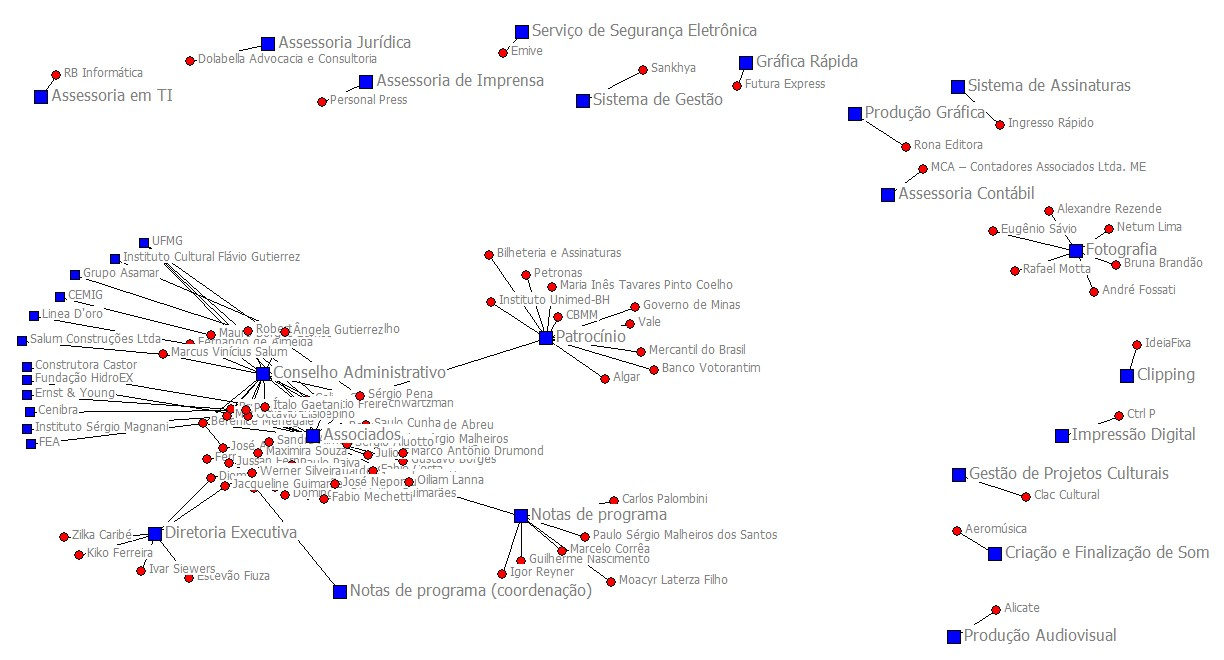
\includegraphics[scale=0.5]{filarmonica_rede2mode.eps}

	%	\fonte{Elaboração do autor com dados disponíveis online \cite{filarmonica2015site}.}

	%	\label{fil2mode}

	%\end{sidewaysfigure}



	É possível perceber a complexidade da teia de recursos que o Instituto mobiliza no decurso de suas atividades cotidianas. Além dos serviços de caráter administrativo como assessorias contábil, jurídica, de TI e outros serviços comuns no campo da cultura como gráfica rápida, fotografia e assessoria de imprensa, é curioso notar alguns serviços que parecem peculiares (embora não exclusivos) ao universo da orquestra. A redação das notas de programa é feita por professores de universidades públicas e pesquisadores vinculados a programas de pós-graduação no exterior. Essas notas de programa geralmente funcionam como um guia ao ouvinte e são inseridas no ``Fortíssimo'', uma publicação mensal da orquestra contendo ainda as biografias dos maestros e solistas convidados e notícias da orquestra. Mais do que um simples programa de concertos, o ``Fortíssimo'' é uma publicação indexada em sistemas nacionais e internacionais de catalogação. As notas de concerto geralmente informam o expectador sobre alguns pontos importantes da biografia do compositor, algumas questões estéticas e estilísticas envolvendo a obra programada para execução além de algumas sugestões de escuta da obra e leitura relacionada. A publicação é distribuída gratuitamente e, ao fim dos concertos, os ouvintes podem retorná-la, caso não queiram guardá-la. O Instituto também mantém uma relação comercial com uma empresa especializada em gestão de projetos culturais. Isso faz sentido se sabemos que uma boa fatia dos recursos captados pela orquestra o são mediante projetos de isenção fiscal.



	
	%Minas Gerais Philharmonic Orchestra began its activities in 2008 led by maestro Fabio Mechetti. It was created from a partnership between Minas Gerais State and \textit{Instituto Cultural Filarmônica}, the maintainer of the orchestra. ``\textit{Instituto Cultural Filarmônica} is a non-profit civil association that has the goals of structuring and maintaining Minas Gerais Philharmonic and promote the diffusion of classical music''\footnote{\fonte{Minas Gerais Philharmonic Website, \url{http://www.filarmonica.art.br/instituto/instituto-cultural-filarmonica/}.}}.
	%The recognition of the \textit{Instituto Cultural Filarmônica} as an \textit{OSCIP}, an Organization of the Civil Society of Public Interest grants them the possibility of signing partnership contracts \cite{minas2017aditivo} with State Government and, therefore, receive investments directly from it. This partnership contract states the amount of resources invested by the government as well as both parts' duties. The document also states the goals and the criteria by which the contract and the orchestra will be evaluated. Those criteria are particularly interesting to us specially because they indicate the weights with which the state conceives artistic quality. Those criteria are divided in 8 large groups and disaggregated according to Table \ref{goals} \cite{filarmonica2017gerencial}:
	
	``O Instituto Cultural Filarmônica é uma associação civil sem fins lucrativos que tem como tarefas estruturar e manter a Orquestra Filarmônica de Minas Gerais e promover a difusão da música clássica'' \footnote{Fonte: Site da Orquestra Filarmônica de Minas Gerais, \url{http://www.filarmonica.art.br/instituto/instituto-cultural-filarmonica/}.}. O reconhecimento do Instituto como uma OSCIP, uma Organização da Sociedade Civil de Interesse Público dá a ele a possibilidade de assinar termos de parceria \cite{minas2017aditivo} com o Governo do Estado e, portanto, receber investimentos diretamente dele. Esse termo de parceria estabelece o volume de recursos investido pelo governo bem como os direitos e deveres de ambas as partes. O documento também estabelece os objetivos e os critérios pelos quais o contrato e a orquestra serão avaliados. Esses critérios são particularmente interessantes para nós especialmente porque eles indicam os pesos com os quais o Estado concebe qualidade artística.  Esses critérios estão divididos em oito grandes grupos conforme a Tabela \ref{goals} \cite{filarmonica2017gerencial}:
	
	

\begin{SingleSpace}
	\begin{footnotesize}
		\begin{center}
			\begin{longtable}{p{6cm} p{7cm} c}
				\caption{Objetivos da Orquestra Filarmônica}\\
				\label{goals}\\
				\hline
				\textbf{Grupo}  & \textbf{Objetivo} & \textbf{Peso} \\
				\hline
				\endfirsthead
				\hline
				\endhead
				\hline
				\endfoot
				\hline
				\multicolumn{3}{l}{Fonte: \cite[p. 3-4]{filarmonica2017gerencial}}\\
				\endlastfoot

				Execução de concertos de assinatura & Número cumulativo de concertos sinfônicos de assinatura no ano de referência & 15 \\
				& Percentual médio de ocupação dos concertos de assinatura de Quinta & 4 \\
				& Percentual médio de ocupação dos concertos de assinatura de Sexta & 4 \\
				& Percentual médio de ocupação dos concertos de assinatura de Sábado & 4 \\
				& Número de assinaturas para séries de concertos sinfônicos & 3 \\
				& Taxa de renovação de assinaturas em relação ao ano anterior & 3 \\
				\hline
				Educação e formação de público para música & Número cumulativo de concertos da série Concertos para a Juventude & 5 \\
				& Percentual médio de ocupação da série Concertos para a Juventude & 4 \\
				& Número cumulativo de concertos da série Concertos Didáticos & 0.5 \\
				& Percentual médio de ocupação da série Concertos Didáticos & 0.5 \\
				& Número cumulativo de concertos da série Música de Câmara & 0.5 \\
				& Percentual médio de ocupação da série Música de Câmara & 0.5 \\
				\hline
				Democratização do acesso à música clássica & Número cumulativo de concertos em praças públicas ou parques na região metropolitana de Belo Horizonte & 0.5 \\
				& Número médio de pessoas nos concertos em praças públicas ou parques da região metropolitana de Belo Horizonte & 0.5 \\
				& Número cumulativo de concertos fora de Belo Horizonte e dentro de Minas Gerais & 0.5 \\
				& Percentual médio de ocupação dos concertos fora de Belo Horizonte e dentro de Minas Gerais & 0.5 \\
				\hline
				Representar o Estado de Minas Gerais nacionalmente e internacionalmente & Número de concertos fora de Minas Gerais & 0.5 \\
				& Percentual médio de opcupação dos concertos fora de Minas Gerais & 0.5 \\
				\hline
				Estímulo à revelação de novos talentos para a música clássica & Realização do \textit{Laboratório de Regência} e o \textit{Festival Tinta Fresca} & 5 \\
				& Percentual médio de ocupação do \textit{Laboratório de Regência} e do \textit{Festival Tinta Fresca} & 4 \\
				\hline
				Prover novas experiências e conhecimento ao corpo arstítico da orquestra & Número cumulativo de regentes convidados e solistas convidados & 5 \\
				\hline
				Financiamento & Financiamento através da bilheteria e assinaturas & 10 \\
				& Financiamento através de patrocínios & 10 \\
				& Dependência dos fundos do contrato de parceria & 10 \\
				\hline
				Gestão da parceria & Percentual de acordo das peças de comunicação da Filarmônica com as direções da OEP & 3 \\
				& Acordo dos processos analisados na chegagem períodica amostral & 3 \\
				& Efetividade do monitoramento do contrato de parceria & 3 \\
			\end{longtable}
		\end{center}
	\end{footnotesize}
\end{SingleSpace}

	
	
	%It is very interesting to notice that if we observe the disaggregated goals, the one with the greatest weight is the cumulative number of signature symphonic concerts but if we observe the groups, the one with the greatest weight is Fund-raising. The signature symphonic concerts are the main activity of the orchestra, the concerts with the most challenging repertoire and that receive the most prestigious guests conductors and soloists. On the other hand, fund-raising states for the management capacities of the maintainer, its capability of running a sustainable of even profitable business.
	
	É muito interessante notar que se observarmos os objetivos desagregados, aquele que possui o maior peso é o número cumulativo de concertos sinfônicos realizados. Entretanto, observando os grupos, o grupo com maior peso é o Financiamento. Os concertos sinfônicos de assinatura são a principal atividade da orquestra. São concertos com o repertório mais desafiador e que recebem os maestros e solistas convidados de maior prestígio. Por outro lado, o grupo de Financiamento se relaciona com as capacidades de gestão da mantenedora, sua capacidade de gerir um negócio sustentável e, até mesmo, lucrativo.
	
	Examinaremos agora os objetivos da orquestra em maiores detalhes.
	
	\subsection{Avaliação dos objetivos da orquestra}
	
	%The first goal group is evaluated regarding the total number of concerts presented in a season, regarding the occupancy of these concerts and regarding the number of signatures\footnote{In Brazil, a signature is a ticket set for all the concerts within a specific series. They can be bought just for a specific series, for combinations of series or for all the concerts in a season.} sold and renewed. The total number of concerts is essentially a quantitative measure of the orchestra's supply. The average percentage of occupancy can be understood, according to the reviewed literature, as a qualitative measure of the concerts. The number of signatures sold and renewed can be understood both as a measure of quality and as a measure of the management capacity of the organization. 
	
	O primeiro grupo de objetivos é avaliado com relação ao número total de concertos apresentados em uma temporada, com relação à ocupação desses concertos e com relação ao número de assinaturas\footnote{Uma assinatura é um conjunto de ingressos para todos os concertos de uma série específica. Eles podem ser comprados apenas para uma série, para uma combinação de séries ou para todos os concertos da temporada.} vendidas e renovadas. O número total de concertos é essencialmente uma medida quantidade da produção da orquestra. O percentual médio de ocupação pode ser entendido, de acordo com a literatura revisada, como uma medida qualitativa dos concertos. O número de assinaturas vendidas e renovadas pode ser entendido tanto quanto uma medida de qualidade quanto uma medida da capacidade gerencial da organização.
	
	%The second group of goals (Education and Formation of Public) is evaluated mainly through one concert series, \textit{Concertos para a Juventude} (Youth concerts). These concerts usually take place on Sunday mornings with low ticket prices and are destined to formation of public. They present ``accessible language to the diffusion of the repertoire of orchestral music'' \cite[p. 9]{filarmonica2017gerencial}. The number of Youth concerts offered and the average percentage of occupancy are the main measures to evaluate this group. The other series that are part of this strategy, the Didactic concerts\footnote{Concerts exclusive to students of the public education system, children's groups social institutions and universities.} and the Chamber concerts\footnote{Concerts with smaller formations, usually string quartets, brass quintets, wood quintets, string trio and piano, etc.} have a very low weight (0.5).
	
	O segundo grupo de objetivos (Educação e Formação de Público) é avaliado principalmente através de uma série de concertos, os Concertos para a Juventude. Esses concertos usualmente acontecem no Domingo pela manhã com ingressos a preços baixos e são destinados à formação de público. Eles apresentam ``linguagem acessível para a difusão do repertório da música orquestral'' \cite[p. 9]{filarmonica2017gerencial}. O número de Concertos para a Juventude realizados e o percentual médio de ocupação são as principais métricas para avaliar esse grupo. As outras séries que fazem parte dessa estratégia, os Concertos Didáticos\footnote{Concertos exclusivos para estudantes da rede pública de ensino, grupos de crianças, instituições sociais e universidades.} e os concertos de Câmara\footnote{Concertos com formações menores, usualmente quartetos de cordas, quintetos de metais, quintetos de madeiras, trio de cordas com piano, etc.} tem um peso mais baixo (0.5).
	
	%The third and fourth groups of goals have a very low impact on the evaluation. These groups are related to orchestra trips to outside the capital of Minas Gerais, to other states and abroad.
	
	O terceiro e o quarto grupos de objetivos tem um impacto baixo na avaliação. Esses grupos são relacionados às viagens da orquestra para fora da capital mineira, outros estados e ao exterior.
	
	%The fifth group is evaluated by the \textit{Laboratório de Regência} (Conducting Lab) and the \textit{Tinta Fresca} Festival. The first event is a conducting masterclass with the orchestra under the guidance of maestro Fabio Mechetti. Nineteen students are selected to participate, fifteen as listener students and four as fully participating students. Those students spend three to four days working with the orchestra on a given repertoire and, at the end, they conduct a concert. The second event is an award to new compositions. The first place winner receives a prize and his composition is included in the next season schedule.
	
	O quinto grupo é avaliado pelo \textit{Laboratório de Regência} e pelo \textit{Festival Tinta Fresca}. O primeiro evento consiste de uma masterclasse de regência com a orquestra sob a orientação do maestro Fabio Mechetti. Dezenove estudantes são selecionados para participar, quinze como ouvintes e quatro como alunos executantes (ou ativos). Estes alunos passam de três a quatro dias trabalhando com a orquestra em um dado repertório e, ao fim, conduzem o concerto de encerramento. O segundo evento consiste de um prêmio para novas composições. O vencedor, além do prêmio, tem sua composição incluída no repertório da temporada seguinte.
	
	%The sixth group is evaluated by a single goal, which is the number of guest conductors and soloists. The partnership contract defines guests conductors as ``Those who do not have permanent contract or employment relationship with the orchestra but come to conduct it or a lyric chorus by invitation of the maintainer'' \cite[p. 40]{minas2017aditivo} and guest soloists as ``instrumentalists or singers who do not have permanent contract or employment relationship with the orchestra and participate on concerts by invitation of the maintainer, playing pieces that require their individual participation'' \cite[p. 40]{minas2017aditivo}. Eventually, musicians that have permanent contract with the orchestra and stand out in the classical music field can be invited to play as a guest soloist.
	
	O sexto grupo é avaliado por um único objetivo, qual seja, o número de regentes e solistas convidados na temporada. O contrato de parceria define regentes convidados como ``Aqueles que não possuem contrato permanente ou vínculo empregatício com a orquestra mas que vem conduzi-la ou o coral lírico por convite da mantenedora'' \cite[p. 40]{minas2017aditivo} e solistas convidados como ``instrumentistas ou cantores que não possuem contrato permanente ou vínculo empregatício com a orquestra e participam de concertos por convite da mantenedora, tocando peças que requerem sua participação individual''  \cite[p. 40]{minas2017aditivo}. Eventualmente, músicos que possuem contrato permanente com a orquestra e se destacam no cenário da música clássica podem ser convidados a se apresentarem como solistas convidados.
	
	%The seventh group, Fund-raising, has the biggest impact on the orchestra evaluation by the State. This group is evaluated by fund-raising through the box office and signatures sold, fund-raising through sponsorship and the ``Dependency on the partnership contract'' score. The first and the second goals are measured in Brazilian Reais (R\$) and the third one is given by a ratio between budget from the partnership contract over total budget.
	
	O sétimo grupo, Financiamento, tem o maior impacto na avaliação da orquestra pelo Estado. Este grupo é avaliado pelo financiamento proveniente da bilheteria e assinaturas vendidas, pelo financiamento através de patrocínio e pela medida de ``Dependência do contrato de parceria''. O primeiro e segundo objetivos são mensurados em reais brasileiros (R\$). O terceiro é definido por uma razão entre o orçamento do contrato de parceria sobre o orçamento total.
	
	%The eighth and last group regards the management of the partnership contract and is evaluated by technical directions regarding marketing material, bureaucratic processes and the monitoring of the contract. We will now take a look at some of this goals in a deeper way.
	
	O oitavo e último grupo está relacionado com a gestão do contrato de parceria e é avaliado por direcionamentos técnicos com relação ao material de marketing, processos burocráticos e monitoramento do contrato. Observaremos agora alguns dos objetivos de maneira mais aprofundada.
	
	\subsection{Principais concertos}
	
	%The ``signature concerts'' are composed by the series called \textit{Allegro}, \textit{Vivace}, \textit{Veloce}, \textit{Presto} and \textit{Fora de Série}. Allegro's concerts happen on thursdays and privilege Romantic and beginning of 20th century repertoire. These concerts are repeated on fridays with the name Vivace. The same logic operates on Presto (thursdays) and Veloce (fridays) concerts. \textit{Fora de Série}'s concerts happen on saturdays and they follow a theme chosen for the season. For instance, 2015's theme was Beethoven, 2016's theme was Mozart, 2017's was Baroque Music and 2018's theme was ``Expeditions'', music from around the globe.
	
	Os ``concertos de assinatura'' são compostos pelas séries chamadas \textit{Allegro}, \textit{Vivace}, \textit{Veloce}, \textit{Presto} and \textit{Fora de Série}. Os concertos da série Allegro acontecem às quintas e privilegiam repertório Romântico e do início do século XX. Esses concertos são repetidos às sextas com o nome Vivace. A mesma lógica opera nos concertos da série Presto (quintas) e Veloce (sexta). Concertos da série \textit{Fora de Série} acontecem aos sábados e normalmente seguem uma temática escolhida para a temporada. Por exemplo, em 2015 o tema escolhido foi Beethoven, em 2016, Mozart, em 2017 música barroca e em 2018 ``Expedições'', música ao redor do mundo.
	
	%Those are the main products of the orchestra, the ones by which it gains its prestige, its status. Also, these concerts are responsible for the biggest part of the orchestras income (.....) %%% MOSTRAR EM UM GRÁFICO.
	
	Estes são os principais produtos da orquestra, aqueles pelos quais ela ganha o seu prestígio, seu status. Além disso, esses concertos são responsáveis pela maior parte das receitas da organização.
	
	
	
	\subsection{Financiamento e dependência do Estado}
	
	%Although one of the most important criteria chosen by the state to evaluate the orchestra is related to its capacity of sustainability, that is, the orchestra's capacity of raising funds from outside the direct investment of the partnership contract, it does not constrain the orchestra to any expectations of less dependency on the State itself. The most part of the investment from private companies is really public money because it is obtained through the laws to encourage culture.
	
	Um dos critérios mais importantes escolhidos pelo Estado para avaliação da orquestra esteja relacionado com sua capacidade de ser sustentável, ou seja, sua capacidade de levantar fundos fora do investimento direto via contrato de parceria. A meta estabelecida para esse indicador é de, no mínimo, 50\%, ou seja, que a parcela de recursos investidos diretamente pelo Governo do Estado seja metade ou menor do que o orçamento total. É importante considerar, entretanto, que a maior parte dos investimentos de companhias privadas é, de fato, dinheiro público visto que são obtidos através de leis de incentivo à cultura mas não contam como tal, contam como investimento privado. No caso da Filarmônica, há uma separação entre o montante financiado por empresas via Leis de Incentivo à Cultura e investimento direto (cf. Tabela \ref{financiamento2017})
	
	A Orquestra Filarmônica contou em 2017 com um financiamento de R\$29.744.228,41 \cite{minas2017aditivo} proveniente de fontes diversificadas. A instituição recebe fundos direto do Governo de Minas, seu principal financiador, de empresas investidoras através de leis de incentivo à cultura e do público pagante.
	
	
	Seu maior financiador, o Governo de Minas é responsável por 61,52\% de seu financiamento total.
	
	% latex table generated in R 3.2.1 by xtable 1.7-4 package
	
	% Thu Oct 15 01:17:07 2015
	
	\begin{table}[!h]
		\IBGEtab{
			\centering
			\caption{Fontes de financiamento da Filarmônica em 2017}
			\label{financiamento2017}
		}
		{\begin{tabular}{rrc}
				\hline
				Fontes & Montantes (R\$) & (\%)  \\
				\hline
				Governo de Minas & 18.298.315 & 61,52 \\ 
				Mercantil do Brasil & 299.000 & 1,005 \\ 
				Banco Votorantim & 229.000 & 0,7699 \\ 
				Anglo Gold Ashanti & 700.000 & 2,353 \\ 
				Instituto Unimed-BH & 370.133 & 1,244 \\ 
				Aliança Energia & 850.000 & 2,858 \\ 
				Picchioni & 180.000 & 0,6052 \\ 
				BTG Pactual & 350.000 & 1,177 \\ 
				Banco Intermedium & 100.000 & 0,3362 \\ 
				CEMIG & 150.000 & 0,5043 \\ 
				Kinross & 688.629 & 2,315 \\ 
				Banco Itaú & 1.000.000 & 3,362 \\ 
				CBMM & 500.000 & 1,681 \\ 
				Telefônica Brasil SA & 320.000 & 1,076 \\ 
				Venda de Concertos & 783.200 & 2,633 \\ 
				Sindicato Hospitais MG & 120.000 & 0,4034 \\ 
				SESI & 485.000 & 1,631 \\ 
				FUNDEP UFMG & 58.200 & 0,1957 \\ 
				Cons. Reg. de Contabilidade MG & 120.000 & 0,4034 \\ 
				Embaixada Americana & 135.291 & 0,4548 \\ 
				Doações livres & 162.255 & 0,5455 \\ 
				Banco Mercantil & 172.000 & 0,5783 \\ 
				YPO - Capítulo BH & 10.000 & 0,03362 \\ 
				Diversas doações & 5.917 & 0,01989 \\ 
				Líder Taxi Aéreo & 200.000 & 0,6724 \\ 
				Bilheteria e Assinaturas & 2.504.687 & 8,421 \\ 
				\hline
				TOTAL & 29.744.228,41 &  \\
				\hline
			\end{tabular}
		}
		{\fonte{Elaboração do autor a partir de \citeonline[p. 2]{minas2017aditivo} e \citeonline[p. 18-20]{filarmonica2017gerencial}.}
		}
	\end{table}
	
	
	
	Fica claro o papel decisivo do Estado como mantenedor da Orquestra Filarmônica de MG. Sem mais de 61,5\% de seu orçamento anual imaginamos que seria bastante difícil para os dirigentes manterem a cota de concertos e os convites a maestros e solistas convidados. 8,4\% do orçamento provém do pagamento de ingressos e assinaturas. Em termos absolutos, o valor representa uma quantia vultuosa se comparado ao campo cultural de um modo geral. Entretanto, representa uma pequena fatia no financiamento da orquestra.
	
	
	
	O restante do financiamento da instituição vem de empresas privadas por meio do mecanismo de incentivo fiscal das leis de incentivo à cultural federal e estadual. Na modalidade de incentivo fiscal, a lei federal (Rouanet) concede às empresas financiadoras de cultura no Brasil uma porcentagem de desconto no Imposto de Renda (IR). A lei estadual de Minas Gerais concede desconto no Imposto sobre Circulação de Mercadorias e Serviços (ICMS). O volume de financiamento adquirido via lei Rouanet corresponde a 18,85\% do total enquanto aquele adquirido via lei estadual, 1,08\% (apenas a empresa Telefônica Brasil SA patrocina por esse meio). Curioso notar que, apesar de as empresas constarem como financiadoras da orquestra, de fato o dinheiro investido provem de isenção fiscal, portanto, dinheiro público. O Estado aparece aqui como um grande centralizador do financiamento da orquestra.
	
	
	\subsection{Repertório e consumo}
	
	%Up to 2014, the orchestra held its main concerts at the \textit{Palácio das Artes} great hall. Usually, the concerts took place once a week or once in two weeks. In 2015, Minas Gerais Hall was inaugurated, a highly technological concert hall that hosts the main Minas Gerais Philharmonic concerts. Also, the opening of this new venue changed the orchestra's supply logic. Concerts began to happen in a weekly basis on thursdays and fridays (cf. ``main concerts'' section) and a new concert series was opened on saturdays.
	
	Esta seção abordará o repertório da orquestra e a taxa de ocupação para as temporadas realizadas em 2015 e 2016. Os dados para a temporada de 2017 ainda não estavam disponíveis no site da orquestra no momento da redação deste trabalho.
	
	Até 2014, a orquestra apresentava seus principais concertos no Grande Teatro do Palácio das Artes. Usualmente os concertos aconteciam uma vez por semana ou uma vez a cada duas semanas. Em 2015 a Sala Minas Gerais foi inaugurada, uma sala de concertos altamente tecnológica que abriga os principais concertos da Filarmônica a partir desse ano. Além disso, a abertura da sala modificou a lógica de produção da orquestra. Os concertos passam a acontecer semanalmente às quintas, sextas e em alguns sábados.
		
	% APRESENTAR ALGUMAS ANÁLISES DE REPERTÓRIO, SAZONALIDADE, DIFERENÇA DE PÚBLICO, ETC......
	
	%For 2015 and 2016, 85\% of all the orchestras concerts happened at Minas Gerais Hall. As we can see in Figure \ref{repertoire-peryear}, the orchestra seems to privilege Romantic and Modern\footnote{Period coding was made by the author. Beethoven was always included in Romantic category. Modern category refers to music of the 20th century.} repertoire.
	
	Para 2015 e 2016, 85\% de todos os concertos da orquestra aconteceram na sala Minas Gerais. Como podemos observar na Figura \ref{repertoire-peryear}, a orquestra parece privilegiar repertório Romântico e Moderno\footnote{A codificação dos períodos de cada obra foi feita pelo autor. Beethoven sempre foi classificado como \textit{romântico}. A categoria \textit{moderno} se refere à música do séc XX.}.
	
	\begin{figure}[!h]
		\centering
		\caption{Repertório da orquestra}
		\label{repertoire-peryear}
		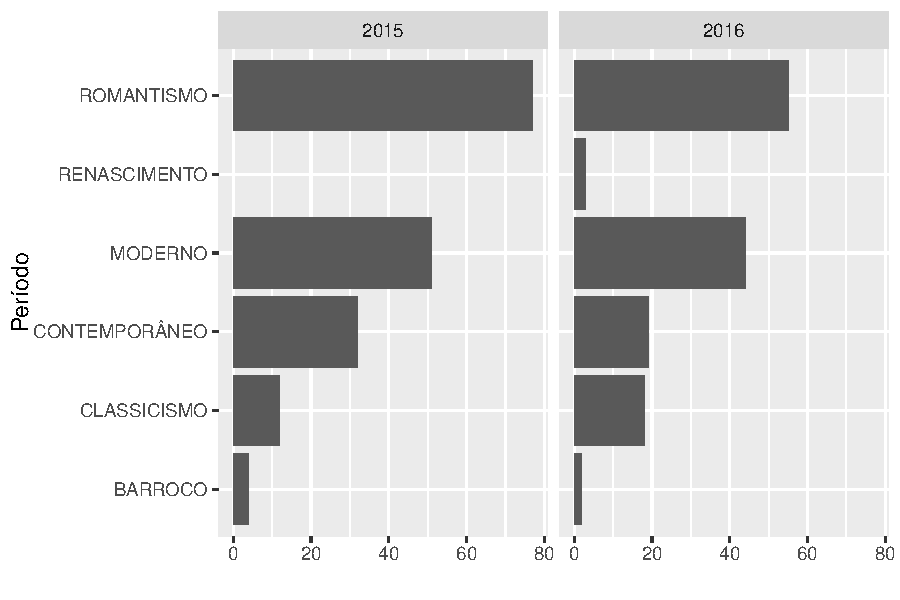
\includegraphics[scale=0.7]{periodo_peryear.pdf}
		\fonte{Elaborado pelo autor usando \textbf{dplyr} e \textbf{ggplot2} \cite{dplyr,ggplot2}.}
	\end{figure}
	
	
	%This proportion stays somewhat stable if we observe the main concert series (with the exception, of course, of the \textit{Fora de Série} thematic series). In Figure \ref{repertoire-perseries}, the Youth Concerts (in the middle column) seems to be the most balanced series. Allegro/Vivace and Presto/Veloce seem quite alike. In 2016, less Classical music has been made in these series. The genre was reserved in that year to \textit{Fora de Série} concerts. 
	
	Essa proporção continua relativamente estável se observamos as principais séries de concertos (com exceção, é claro, da \textit{Fora de Série} que é temática). Na Figura \ref{repertoire-perseries}, os Concertos para a Juventude (na coluna central) parecem ser a série mais balanceada. Allegro/Vivace e Presto/Veloce possuem grande similaridade. Em 2016, menos repertório clássico foi feito nessas séries. O gênero ficou reservado naquele ano para a série \textit{Fora de Série}.
	
	\begin{figure}[!h]
		\centering
		\caption{Repertório por série}
		\label{repertoire-perseries}
		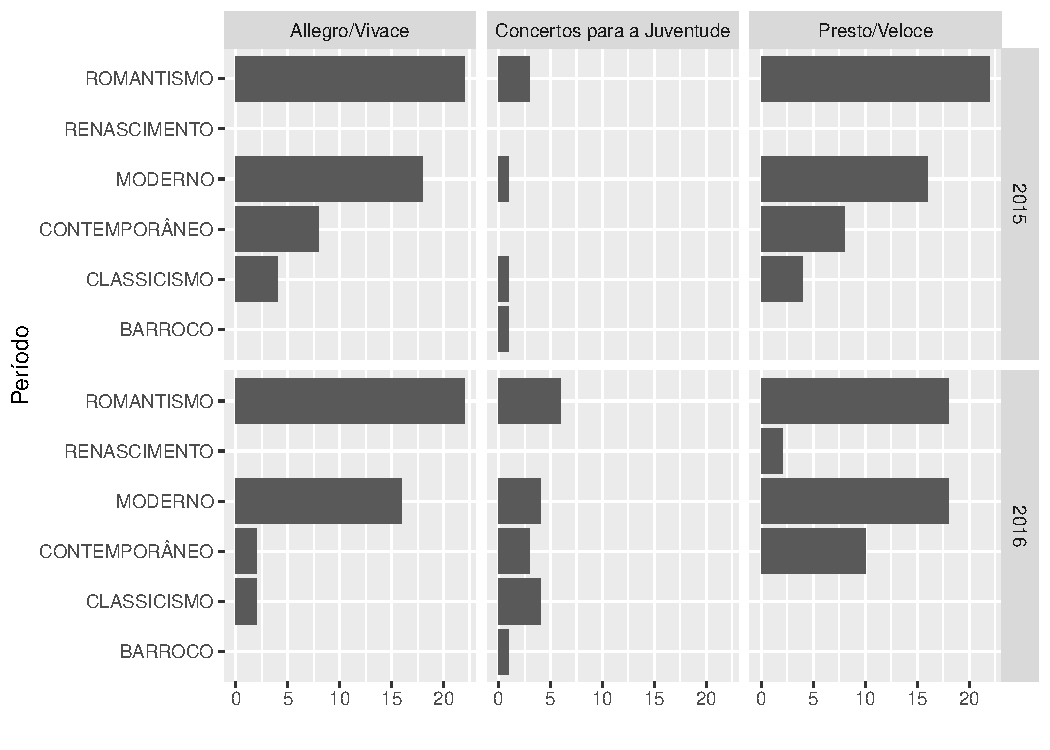
\includegraphics[scale=0.7]{periodo_perserie_year.pdf}
		\fonte{Elaborado pelo autor usando \textbf{dplyr} e \textbf{ggplot2} \cite{dplyr,ggplot2}.}
	\end{figure}
	
	
	%In order to investigate the consumption, the 2016 results report gives us the number of seats available and the number of tickets sold to calculate the occupancy rate. At first, we are tented to believe that the consumption of the concerts is mostly related by the chosen repertoire which, therefore, would reflect on the concert series. Nevertheless, because of the change in the concerts offering since 2015, we believe that the weekday has a larger impact on consumption. Linear models showed that the series has a bigger explanatory power on consumption (cf. Table \ref{concert-consumption-models}). The models were estimated with the occupancy rate as the dependent variable and only for 2016\footnote{Unfortunately, the number of seats available is only reported in 2016's reports. In order to make our further analysis more robust, we estimated the seats available for 2015 given that the venues, the weekdays of the concerts and the series were the same as 2016. A technical description of the estimation procedure is given in the appendix.}.
	
	Para investigar o consumo, o relatório de resultados de 2016 da Filarmônica nos dá o número de assentos disponíveis e o número de ingressos vendidos para calcular a taxa de ocupação. Numa primeira análise, somos tentados a acreditar que o consumo de concertos está altamente relacionado com o repertório escolhido o qual, portanto, refletiria nas séries de concertos. Contudo, por causa da mudança na oferta dos concertos desde a inauguração da Sala Minas Gerais em 2015, acreditamos que o dia da semana tem maior impacto no consumo. A figura \ref{fig:txocup} mostra a distribuição da taxa de ocupação por série de concertos e por dia da semana.

        \begin{figure}[!ht]
          \centering
          \caption{Taxa de ocupação por série e dia da semana}
          \label{fig:txocup}
          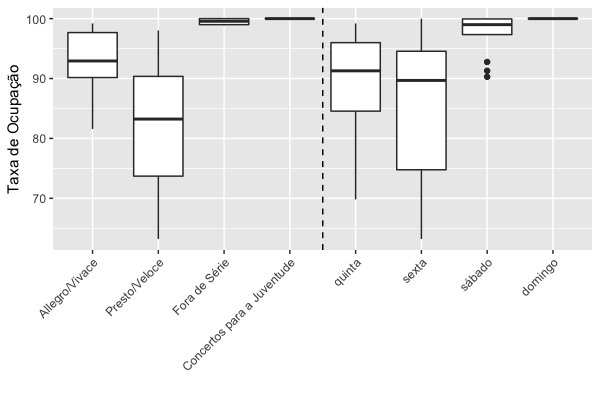
\includegraphics[scale=0.6]{taxa_ocup_dia_serie}
        \end{figure}

        Para testar essa hipótese, estimamos testes de média para todos os pares de dias da semana (cf. Tabela \ref{tab:tdia}) e séries de concerto (cf. Tabela \ref{tab:tserie}). É possível notar que os pares de séries de concerto apresentam mais diferenças de média estatisticamente significativas do que pares de dias da semana, o que indica que a ocupação está mais relacionada à escolha do repertório e desenho da série do que ao dia da semana.


        %estimamos dois modelos de regressão linear tendo a taxa de ocupação como variável dependente. O primeiro modelo utilizava os dias da semana como preditores. O segundo utilizava as séries de concerto como preditores. Comparando as medidas de ajuste do modelo ($R^2$ ajustado e RMSE), foi possível identificar que as séries de concerto possuem maior poder explicativo sobre o consumo ($R^2$ ajustado calculado para o modelo com as séries foi o dobro - 0.5 - que a mesma estatística de ajuste calculada para o modelo com os dias da semana - 0.25. O RMSE daquele modelo também foi menor indicando melhor ajuste). Os resultados dos dois modelos estão apresentados na  Tabela \ref{concert-consumption-models}. Os modelos foram estimados usando dados de 2016\footnote{Infelizmente, o número de assentos disponíveis foi reportado apenas no relatório de 2016, não em 2015.}.




        % Pairwise t testes
        % latex table generated in R 3.5.3 by xtable 1.8-3 package
        % Wed May  1 22:57:38 2019
        \begin{table}[ht]
          \ibgetab{
          \centering
          \caption{Testes de média pareados - dias da semana (p-values)}
          \label{tab:tdia}
          }
          {\begin{tabular}{r|rrr}
            \hline
            & Domingo & Quinta & Sábado \\ 
            \hline
            Quinta & 0.05 &  &  \\ 
            Sábado & 0.55 & 0.05 &  \\ 
            Sexta & 0.00 & 0.16 & 0.00 \\ 
            \hline
           \end{tabular}
         }
         {\fonte{Elaboração do autor.}}
        \end{table}



        % latex table generated in R 3.5.3 by xtable 1.8-3 package
        % Wed May  1 22:57:38 2019
        \begin{table}[ht]
          \ibgetab{
          \centering
          \caption{Testes de média pareados - séries de concertos (p-values)}
          \label{tab:tserie}
          }
          {\begin{tabular}{r|p{2.5cm}p{2.5cm}p{2.5cm}}
             \hline
             & Allegro/Vivace & Concertos para a Juventude & Fora de Série \\ 
             \hline
             Concertos para a Juventude & 0.09 &  &  \\ 
             Fora de Série & 0.07 & 0.89 &  \\ 
             Presto/Veloce & 0.00 & 0.00 & 0.00 \\ 
             \hline
           \end{tabular}
         }
         {\fonte{Elaboração do autor.}}
        \end{table}

        
\begin{comment}	
	\begin{table}[!h]
		\ibgetab{
			\centering
			\caption{Consumo de concertos - Modelos Lineares - Dependente: Taxa de Ocupação}
			\label{concert-consumption-models}
		}
		{\begin{tabular}{l c c }
				\hline
				& Modelo 1 & Modelo 2 \\
				\hline
				(Intercepto)                                        & $85.28^{***}$ & $93.36^{***}$  \\
				& $(1.84)$      & $(1.46)$       \\
				\textbf{Dia da semana} & & \\
				Domingo & $14.72^{***}$ &                \\
				& $(3.98)$      &                \\
				Quinta  & $4.59$        &                \\
				& $(2.58)$      &                \\
				Sábado  & $12.15^{***}$ &                \\
				& $(3.10)$      &                \\
				\textbf{Série de Concertos} & & \\
				Concertos para a Juventude                    &               & $6.64^{*}$     \\
				&               & $(3.21)$       \\
				Fora de Série                                 &               & $6.13^{*}$     \\
				&               & $(2.65)$       \\
				Presto/Veloce                                 &               & $-11.26^{***}$ \\
				&               & $(2.05)$       \\
				\hline
				R$^2$                                              & 0.28          & 0.53           \\
				Adj. R$^2$                                         & 0.25          & 0.50           \\
				Num. obs.                                          & 63            & 63             \\
				RMSE                                               & 8.64          & 7.01           \\
				\hline
				\multicolumn{3}{l}{\scriptsize{$^{***}p<0.001$, $^{**}p<0.01$, $^*p<0.05$}}
			\end{tabular}
		}
		{\fonte{Elaborado pelo autor.}}
	\end{table}
\end{comment}	
	
	% Talk about occupancy rate by series. Run the analysis in R.
	%On Table \ref{occupancy-table} we can observe that weekend concerts have higher occupancy rate than on weekdays. ....................
	
	Na Tabela \ref{occupancy-table} podemos observar que os concertos de fim de semana possuem uma taxa maior de ocupação em relação aos concertos realizados durante a semana. Os concertos de domingo tiveram lotação em todas as apresentações em 2016. O sábado é o segundo melhor dia de concertos com relação à ocupação. As sextas tem a média e a mediana de ocupação mais baixas.
	
	% latex table generated in R 3.4.3 by xtable 1.8-2 package
	% Mon Jan 15 14:19:21 2018
	\begin{table}[!h]
		\ibgetab{
			\centering
			\caption{Taxa de Ocupação -- 2016}
			\label{occupancy-table}
		}
		{\begin{tabular}{lrrrrr}
				\hline
				\multicolumn{6}{l}{\textbf{Por Série de Concertos}} \\
				\hline
				Série & mean & median & sd & min & max \\ 
				\hline
				Allegro/Vivace & 93.38 & 92.93 & 4.59 & 81.56 & 99.20 \\ 
				Concertos para a Juventude & 100.00 & 100.00 & 0.00 & 100.00 & 100.00 \\ 
				Fora de Série & 99.78 & 100.00 & 0.42 & 98.86 & 100.00 \\
				Laboratório de Regência & 98.93 & 98.93 & 0.00 & 98.93 & 98.93 \\ 
				Presto/Veloce & 82.64 & 84.56 & 10.43 & 63.20 & 98.03 \\ 
				\hline
				\multicolumn{6}{l}{\textbf{Por Dia da Semana}} \\
				\hline
				Dia  & mean & median & sd & min & max \\
				\hline
				Domingo  & 100.00 & 100.00 & 0.00 & 100.00 & 100.00 \\ 
				Quinta & 89.88 & 91.28 & 7.31 & 69.81 & 99.20 \\ 
				Sábado & 98.56 & 100.00 & 2.90 & 90.29 & 100.00 \\  
				Sexta & 86.81 & 90.14 & 12.27 & 63.20 & 100.00 \\ 
				\hline
			\end{tabular}
		}
		{\fonte{Elaborado pelo autor.}}
	\end{table}
	
	
	
	\subsection{Custos}
	
	De acordo com o dirigente entrevistado da orquestra Filarmônica de MG, a folha de pagamento do pessoal corresponde a 70\% do orçamento total da orquestra sendo que 64\% são destinados à folha de pagamento dos músicos e 6\% ao pagamento do pessoal do Instituto Cultural Filarmônica. Cerca de 17\% do orçamento total é destinado à direção artística.
	
	Para que os concertos aconteçam há vários custos relacionados à parte artística que vão além da folha da pagamento dos músicos e convidados. Além do cachê dos músicos e convidados há despesas com passagens, transporte, hospedagem e custos de comunicação. Isso ocupa 20\% do orçamento total. Os 10\% restantes ficam destinados a custos operacionais da organização.
	
	\subsection{Motivação}
	
	Quando indagado sobre os incentivos que a orquestra dá aos músicos para que eles se sintam motivados e felizes em relação ao trabalho, o dirigente entrevistado respondeu que essa é uma preocupação central na gestão da Filarmônica. Como medidas de motivação, o entrevistado citou um \textit{salário competitivo no mercado} visto que o salário inicial do músico que toca na Filarmônica é um dos melhores do país; pagamento de adicional para manutenção de instrumentos, adicional a título de seção de imagem além de plano de saúde, auxílio alimentação e seguro de vida.
	
	Para além desses incentivos financeiros, o dirigente comenta que a orquestra convida os músicos a participarem do destino da organização realizando uma comunicação direta e transparente com eles e deixando-os a par de todas as dificuldades e desafios da orquestra como organização. Eles são informados constantemente sobre os processos de captação de recursos da organização e convidados a apresentar ideias criativas que ajudem na gestão ou na própria captação.
	
	A Sala Minas Gerais em si configura, para o entrevistado, outro incentivo para que os músicos se sintam motivados. A orquestra trabalha para que os músicos desenvolvam um sentimento de pertencimento ao local, que o sintam como a ``casa'' da orquestra e um local onde eles tanto realizam as performances quanto utilizam como local de estudo e preparação do repertório. Eles podem utilizar os diversos espaços da sala para isso. Há também uma sala na parte administrativa do prédio reservada para a associação dos músicos da Filarmônica.
	
	Por fim, os músicos recebem constantemente convites para se apresentarem como solistas ou em concertos de câmara promovidos pela orquestra.
	
	
	\subsection{A rede da orquestra}
	
	Segundo o dirigente entrevistado, a orquestra Filarmônica possui intensa relação com a economia criativa demandando serviços que extrapolam a função musical. A orquestra exerce grande impacto no setor hoteleiro, nos restaurantes e na rede gastronômica da cidade, no setor de transportes, empresas de estruturas de palco, sonorização e iluminação, no setor de aviação e alguns outros.
	
	Na Figura \ref{rede-filarmonica} abaixo, representamos a rede egocentrada da orquestra Filarmônica reconstruída a partir da entrevista realizada. A rede está colorida a partir do tipo de relações que a orquestra possui.
	
	\begin{figure}[!ht]
		\centering
		\caption{Rede Egocentrada da Orquestra Filarmônica}
		\label{rede-filarmonica}
		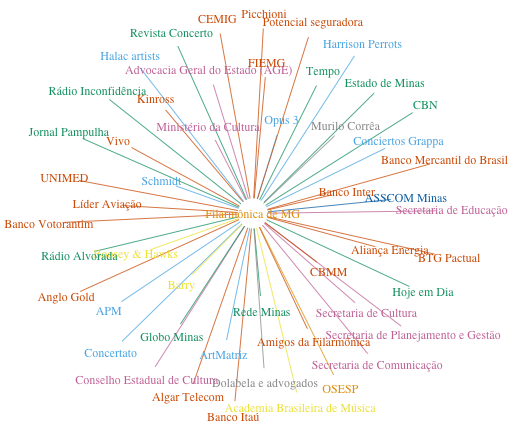
\includegraphics[scale=.7]{rede_filarmonica.png}
		\fonte{Elaboração do autor usando linguagem \textbf{R} e \textbf{igraph} \cite{rlanguage,igraph}}
	\end{figure}
	
	Podemos observar relações de patrocínio, parceria para divulgação, mediação de contratos com músicos e artistas convidados, relações com diversos órgãos do Estado, locação ou compra de partituras e material de orquestra, terceirização de serviços meio (advogados e gravação/sonorização), aconselhamento institucional e parceria institucional. As frequências observadas para cada tipo de relação estão apresentadas na Tabela \ref{relacoes-filarmonica}. 
	
	
	% latex table generated in R 3.5.1 by xtable 1.8-3 package
	% Wed Jan  2 18:07:14 2019
	\begin{table}[!h]
		\ibgetab{
		\centering
		\caption{Tipos de relações da Filarmônica}
		\label{relacoes-filarmonica}
	}
		{\begin{tabular}{lr}
			\hline
			\textbf{Relação} & \textbf{Frequência} \\ 
			\hline
			Patrocínio &  18 \\ 
			Divulgação &  10 \\ 
			Contratos &   8 \\ 
			Relação com o Estado &   7 \\ 
			Locação ou compra &   3 \\ 
			Terceirização de serviço &   2 \\ 
			Aconselhamento &   1 \\ 
			Parceria institucional &   1 \\ 
			\hline
		\end{tabular}
	}
	{\fonte{Elaboração do autor a partir da entrevista realizada com o dirigente da orquestra.}}
	\end{table}

	É interessante notar que dentre as relações com o Estado mencionadas estão a Secretaria de Cultura, a Secretaria de Educação, a Secretaria de Planejamento e Gestão, a Secretaria de Comunicação, a Advocacia Geral do Estado (AGE) e o Conselho Estadual de Cultura que fazem parte do Governo de Minas. Ao nível da União, foi citado o Ministério da Cultura, órgão gestor da Lei Federal de Incentivo à Cultura (Lei Rouanet) da qual a Filarmônica é beneficiária na captação de recursos junto às empresas por isenção fiscal. Como vimos acima, os recursos captados via Lei Rouanet são de grande importância para a manutenção da orquestra visto sua grande parcela no total. Embora a ASSCOM (Assessoria de Comunicação Social) tenha sido citada, ela aparece como a parceria institucional da orquestra.
	
	O dirigente apontou uma relação de aprendizado organizacional estabelecida com a OSESP, a Orquestra Sinfônica do Estado de São Paulo. Foi relatado que é comum a realização de \textit{benchmarking}'s\footnote{Prática de aprendizado organizacional. No caso específico relatado, trata-se do \textit{benchmarking de cooperação}, situação onde uma empresa de renome ou grande prestígio abre seus processos para que outra organização possa aprender com ela (cf. \url{https://endeavor.org.br/estrategia-e-gestao/benchmarking/}).} com eles para verificar técnicas de gestão, captação de recursos dentre outras especificidades.
	
	Entre seus patrocinadores estão financeiras e bancos, mineradoras, empresas de energia, telecomunicações, aviação, medicina, uma associação, uma seguradora, e a Federação das Indústrias. A rede, de um modo geral, é diversificada quanto ao tipo de empresas e quanto às relações nela mencionadas. Dentre as redes egocentradas identificadas pelas entrevistas com os dirigentes, a rede da Filarmônica é a mais complexa.
	


	\section{Orquestra Sinfônica de Minas Gerais}

	A Orquestra Sinfônica de Minas Gerais difere das demais pois não possui a autonomia de gestão que as demais possuem. A Sinfônica faz parte da Fundação Clóvis Salgado, e é gerida por ela. Todas as parcerias e contratos da orquestra não são feitos por ela mesma, mas pela Fundação. Desse modo a Orquestra Sinfônica não pode receber financiamento de empresas por meio das leis de incentivo à cultura mas recebe apenas repasses diretos do Governo do Estado por meio de termos de parceria.
	
	De acordo com o dirigente entrevistado, no último governo de Fernando Pimentel foram criados os termos de parceria para que a Fundação Clóvis Salgado fosse retirada do mercado de captação de recursos via leis de incentivo à cultura. Para o entrevistado, a Fundação é um organismo cultural muito forte e com uma história muito bem consolidada no Estado de Minas o que o empresariado tende a valorizar. Isso criava uma competição desigual com outros empreendedores menores que competiam pelos mesmos recursos. O Estado, portanto, repassa via termos de parceria praticamente a totalidade do orçamento anual da orquestra. Cerca de 90\% do orçamento da orquestra veio diretamente do Estado nos últimos três anos. Não obstante, o dirigente comenta que a arrecadação era maior quando era realizada através das leis de incentivo à cultura.
	
	A gestão financeira dos recursos é realizada pela APPA (Associação Pró-Cultura e Promoção de Artes). A APPA é um Organização da Sociedade Civil de Interesse Público (OSCIP) externa à Fundação Clóvis Salgado escolhida por licitação. É curioso notar que os termos de parceria celebrados entre a APPA e o Governo do Estado não preveem repasses apenas para a orquestra mas para toda a Diretoria Artística da Fundação Clóvis Salgado a qual deve gerir, com esse recurso, todos os corpos artísticos da instituição, a saber, a Orquestra Sinfônica, o Coral Lírico de MG e a Cia. de Dança.
	
	A orquestra é composta, em sua parte artística, pelo maestro, pelo maestro assistente e por setenta e três músicos no total. Desses músicos, 75,34\% (cinquenta e cinco músicos) são funcionário públicos estatutários, ou seja, o seu salário é pago diretamente pelo Governo do Estado; são funcionário do Estado. Os outros 24,64\% (dezoito músicos) são contratados e pagos pelo orçamento da Diretoria Artística. Segundo o dirigente entrevistado, os músicos contratados são parte essencial da orquestra a qual não consegue funcionar sem eles devido ao número mínimo de instrumentos necessários às obras selecionadas para compor a programação da temporada. O gerente da orquestra estaria ao lado do maestro na estrutura hierárquica da organização. Abaixo do gerente há a secretaria, os arquivistas e montadores.
	
	É curioso notar que, no caso da Sinfônica, o maestro é contratado. Isso permite a ele ter o poder decisório de questões artísticas da orquestra. Qualquer dúvida ou discussão artística no grupo é direcionada a ele para que a decisão seja tomada. Entretanto, pelo regime de contratação, o maestro não possui autoridade jurídica sobre os músicos, ou seja, não é responsável por nenhuma questão administrativa que os envolva, já que não é funcionário da organização. A coordenação administrativa dos músicos é feita pelo gerente e, em segunda instância, pela direção artística.
	

	\subsection{Avaliação dos objetivos da orquestra}
	
	A Orquestra Sinfônica tem também os relatórios de avaliação dos termos de parceria disponibilizados no site da Fundação Clóvis Salgado\footnote{\url{http://fcs.mg.gov.br/institucional/termos-de-parceria/}} e no site de sua gestora, a APPA\footnote{\url{https://appa.art.br/termos-de-parceria/diart-relatorios/}}. A avaliação da orquestra é realizada com base em cinco grupo que possuem nove indicadores. Eles estão apresentados na Tabela \ref{objetivos-sinfonica}.
	
	
	\begin{table}[!h]
		\ibgetab{
		\centering
		\caption{Avaliação dos objetivos da Orquestra Sinfônica}
		\label{objetivos-sinfonica}	
	}
		{\begin{tabular}{p{6cm} p{7cm} c}
				\hline
				\textbf{Grupo}  & \textbf{Objetivo} & \textbf{Peso} \\
				\hline
				Apoio à produção artística da Orquestra Sinfônica de MG & Nº de apresentações das séries Sinfônica ao Meio Dia, Sinfônica em Concerto, Concertos Comentados e Concurso Jovens Solistas. & 10\% \\
				\hline
				Apoio à produção artística do Coral Lírico de MG & Nº de apresentações das séries Lírico ao Meio Dia e Lírico em Concerto. & 10\% \\
				 & Nº de apresentações das séries Líricas: Sacro e Sarau & 10\% \\
				\hline
				Apoio à produção artística da Cia. de Dança Palácio das Artes & Nº de atividades do CDPA & 10\% \\
				\hline
				Apoio à produção artística integrada & Nº de apresentações conjuntas OSMG e CLMG & 15\% \\
				   & Nº de apresentações da série Sinfônica Pop & 15\% \\
				   & Nº de récitas de Óperas & 20\% \\
				\hline
				Gestão da entidade parceira & Percentual de conformidade dos processos analisados na checagem amostral periódica & 5\% \\
				   & Efetividade do monitoramento do Termo de Parceria & 5\% \\
				\hline				
			\end{tabular}
	}
		{\fonte{\cite[p. 3]{sinfonica2017gerencial}}}
	\end{table}


	Os objetivos da Sinfônica, assim como os da Filarmônica, estão intrinsecamente ligados à realização de sua principal atividade fim, os espetáculos mas, como podemos observar, privilegia as ações conjuntas dos corpos artísticos, a saber, os concertos da Orquestra Sinfônica junto ao Coral Lírico, os concertos da série Sinfônica Pop e as temporadas de Ópera do Palácio das Artes. As montagens de óperas são, de fato, as maiores produções da Orquestra Sinfônica e as que trazem consigo maior prestígio e reconhecimento\footnote{No fim de 2018, o Palácio das Artes teve a sua montagem da ópera \textit{La Traviata} de G. Verdi como finalista do prêmio Lauro Machado da Revista Concerto, uma das principais publicações especializadas do país. Embora não tenha sido a vencedora no julgamento da comissão avaliadora, foi a mais votada na participação do público (cf. \url{https://concerto.com.br/noticias/premio-concerto-2018}).}.
	
	Para além da realização das séries de concertos e apresentações dos três corpos artísticos da Fundação Clóvis Salgado, o Termo de Parceria avalia a gestão da entidade parceira com 10\% de peso acumulado para o grupo. É possível avaliar, observando  a Tabela \ref{objetivos-sinfonica}, que quanto à Orquestra Sinfônica, o que o Estado entende como prioridade são as récitas de Ópera e, em segundo lugar, as apresentações conjuntas.
	
	
	O orçamento da Orquestra Sinfônica acordado no Termo de Parceria foi de R\$7.830.346,05 para o cumprimento dos objetivos elencados na Tabela \ref{objetivos-sinfonica}\cite{appa2017parceria} entre junho de 2017 e dezembro de 2019. Segundo o dirigente entrevistado, desse montante não é extraído o pagamento dos músicos efetivos da orquestra, visto que são funcionários do Estado. Com ele são pagos os dezoito músicos contratados da orquestra, maestros, cantores contratados, bailarinos contratados, montadores contratados e toda a parte de produção artística do ano.  
	
	\subsection{Séries de concertos}
	
	A Orquestra Sinfônica possui quatro séries de concertos e, além disso, apresentações conjuntas com o Coral Lírico de Minas Gerais, a série Sinfônica Pop e as Óperas.
	
	A série Sinfônica em Concerto consiste da principal série de concertos da orquestra e traz variadas formações e tipos de repertório. O preço comum do ingresso é 30 reais. Os Concertos Comentados são uma série de caráter formativo mais voltada ao público jovem visando sensibilizá-los como espectadores e consumidores das apresentações artísticas. É privilegiado um repertório mais acessível, que possa ser explicado e seja mais didático; que mostre a formação da orquestra ou que possa contar alguma história através do repertório escolhido. Estes concertos são gratuitos. Os Concertos ao Meio Dia acontecem nesse horário no grande teatro do Palácio das Artes e tem, geralmente, o mesmo repertório dos Concertos Sinfônicos. Esta série, porém, tem entrada gratuita. O Concurso Jovens Solistas configura um incentivo para jovens instrumentistas e cantores. A premiação do concurso consiste da participação dos vencedores em um concerto com a Orquestra Sinfônica e a entrega de uma placa simbólica que registra o prêmio. Este concerto também é gratuito ao público \cite{appa2017parceria}.
	
	Os concertos em conjunto realizados pela Orquestra Sinfônica e pelo Coral Lírico são similares àqueles da série Sinfônica em Concerto mas com repertório que privilegie a formação de orquestra e coro. Os ingressos também são vendidos a 30 reais. A série Sinfônica Pop privilegia o repertório da música popular brasileira e normalmente acontece em conjunto com artistas convidados de renome\footnote{Zizi Possi, Wagner Tiso, Nana Caymmi, João Bosco, Gal Costa, Milton Nascimento, Lenine, Ivan Lins, Elba Ramalho são alguns dos convidados.}. Nesses concertos são realizados arranjos originais encomendados pela APPA. As produções de ópera quase sempre envolvem todos os corpos artísticos da instituição e exigem uma grande mobilização administrativa quanto à produção e à gestão pois trata-se de um empreendimento mais complexo. Dessas produções fazem parte as récitas no grande teatro do Palácio das Artes cujos ingressos são comercializados a sessenta reais e Concertos no Parque que são usados essencialmente para divulgar as temporadas de ópera e em seu repertório incluem trechos da ópera a ser executada. Os concertos no parque são gratuitos \cite{appa2017parceria}. Segundo o dirigente entrevistado, há também uma preocupação em realizar um repertório operístico que seja novo para a cidade de Belo Horizonte. ``Nos últimos anos fizemos seis óperas, quatro delas foram estreias em Minas Gerais'' (\textit{Dirigente Entrevistado}). Por fim, o Termo de Parceria propõe uma inovação na execução do repertório sinfônico de modo que sejam elaboradas novas formas de apresentação envolvendo os três corpos artísticos da instituição. 
	
	\subsection{A rede da orquestra}
	
	Das relações que a Orquestra Sinfônica de Minas Gerais possui, conseguimos identificar relações de patrocínio (com a Vivo, Instituto Unimed-BH e a FHEMIG), relações de apoio cultural (com a Rede Minas, Globo Minas e a Rádio Inconfidência), uma relação de colaboração cultural (com a Copasa) e uma parceria institucional (com a Orquestra Sinfônica da Polícia Militar). A rede identificada da Orquestra Sinfônica é bem menos complexa em relação à rede da Filarmônica mas já é possível perceber alguns nós em comum. A rede egocentrada da Orquestra Sinfônica está representada na Figura \ref{rede-sinfonica}.
	
	\begin{figure}[!ht]
		\centering
		\caption{Rede Egocentrada da Orquestra Sinfônica}
		\label{rede-sinfonica}
		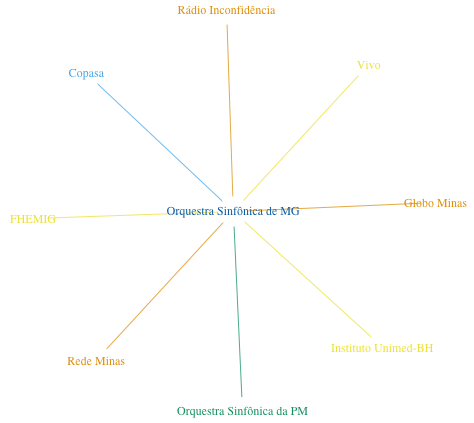
\includegraphics[scale=.7]{rede_sinfonica.png}
		\fonte{Elaboração do autor usando linguagem \textbf{R} e \textbf{igraph} \cite{rlanguage,igraph}}
	\end{figure}

	Dentre as relações observadas é curioso notar a parceria institucional com a Orquestra Sinfônica da Polícia Militar. Segundo o dirigente entrevistado, a Sinfônica tem realizado alguns concertos conjuntos com a Sinfônica da PM com as duas orquestras no palco. De acordo com o entrevistado a experiência tem sido extremamente positiva.


	\subsection{Motivação}
	
	O caso da Sinfônica é singular quanto à motivação de seus músicos. De acordo com o dirigente entrevistado, os músicos da Orquestra Sinfônica de Minas Gerais possuem o salário mais baixo entre as orquestras do Brasil, o que, obviamente, cria um grau de insatisfação muito grande e gera inúmeras dificuldades para a condução do trabalho artístico. Além disso, a incapacidade de fazer mudanças na equipe parece fazer com que o trabalho obtenha um limite qualitativo delimitado cuja transposição é bastante difícil.
	
	Na Orquestra Sinfônica acontecem convites para que os músicos se apresentem como solistas de alguns concertos específicos. Entretanto, essa prática esbarra na burocracia condicionada pelo modelo de contratação dos músicos. Pelo fato do músico da orquestra ser um funcionário público, ele não pode ser remunerado em nada além do seu salário para tocar como solistas em um concerto. Quando há interesse em fazer um convite dessa natureza é necessário negociar outros aspectos, dar outro tipo de de gratificação ao músico.
	
	Segundo o dirigente entrevistado, ``qualquer estrutura que engesse um grupo artístico faz com que esse grupo artístico sobreviva mas não evolua o tanto que precisa. O funcionarismo público garante a existência e a sobrevivência do grupo mas o engessa em inúmeros aspectos''. A orquestra se mobiliza para que haja melhoria salarial, melhoria na qualidade artística mas esses esforços acabam por não obter os resultados desejados devido ao alto grau de burocracia na qual a organização está inserida. Para que a orquestra possa avançar qualitativamente, seria necessário, de acordo com o dirigente entrevistado, maior maleabilidade e liberdade de atuação.
	
	
	
	
	
	\section{Orquestra SESIMINAS}
	
	A Orquestra de Câmara SESIMINAS é um caso diferente dos demais apresentados a começar pela natureza da própria relação da orquestra com o SESI. Os músicos não são funcionários do SESI, a orquestra é terceirizada. De acordo com o dirigente entrevistado, quando a orquestra foi fundada em 1986, os músicos eram então funcionários. Em dezembro de 1995 foi criada a MUSICOOP (Cooperativa dos Músicos Profissionais de Minas Gerais), uma cooperativa na qual os músicos são associados. Dessa cooperativa fazem parte os músicos, o presidente da MUSICOOP e gerente da orquestra e, como contratados da cooperativa, uma secretária e um arquivista. O SESI, o principal financiador da orquestra, contrata um número de concertos específicos da MUSICOOP anualmente e esse contrato configura, basicamente, o orçamento anual da organização. As únicas exceções são o maestro titular e o maestro assistente, ambos funcionários do SESI, encarregados da gestão artística do grupo, não da gestão administrativa.
	
	O SESI (Serviço Social da Indústria) é uma entidade que é parte do sistema FIEMG (Federação das Indústrias do Estado de Minas Gerais) e destina-se a oferecer ``programas e serviços para elevar a qualidade de vida dos trabalhadores e seus familiares\footnote{\url{https://www7.fiemg.com.br/sesi/mais-sesi}}''. A FIEMG é um sindicato patronal. Ela recebe a contribuição sindical patronal das indústrias em Minas Gerais pagas de acordo com a classificação do capital social em janeiro. A contribuição é espontânea e destinada a todas as empresas brasileiras. A contribuição possui previsão nos artigos 578, 579 e 580 da Consolidação das Leis do Trabalho (CLT)\footnote{\url{http://www.fiemg.com.br/hotsites/contribuicao_sindical/}}. O SESI, portanto, obtém suas receitas dessa contribuição sindical.
	
	Com a crise financeira que atingiu o país e a ausência de obrigatoriedade do pagamento compulsório da contribuição sindical patronal alterada pela lei nº 13.467/2017 (conhecida como reforma trabalhista), o SESI se encontra numa situação de difícil gestão devido à incerteza da arrecadação de seus recursos. Obviamente, como o SESI é a principal (praticamente única) financiadora da orquestra, esta se vê em um cenário de cortes crescentes e incertezas. 
	
	Para além do patrocínio do SESI via contrato, a orquestra também possui parcerias para a realização de eventos específicos, convites para performances e concertos para além do que já estava previsto na programação. Esses convites são normalmente realizados pelas indústrias conveniadas. Nesses casos, a instituição convidante deve arcar com os custos logísticos do concerto. Esses convites, porém são bastante pontuais. A organização também realiza alguns concertos fora daqueles contratados pelo SESI, embora também bastante pontuais. Nesses casos, a orquestra realiza a captação de financiamento pelas leis de incentivo à cultura e se apresenta não como Orquestra SESIMINAS mas como Orquestra MUSICOOP. Os projetos de gravação dos CD's da orquestra, por exemplo, foram realizados dessa forma.
	
	O SESI contratou, em 2017, 40 concertos da MUSICOOP. Para a realização destes 40 concertos, o orçamento anual foi de aproximadamente 1 milhão de reais. Em 2018 o SESI contratou 30 concertos o que gerou um orçamento anual de cerca de 750 mil reais e para 2019, estão previstos 21 concertos e um orçamento de cerca de 550 mil reais. Desse orçamento, cerca de 90\% fica a cargo do pagamento dos músicos. As demais despesas são contas fixas da organização (o salário dos dois funcionários, água, energia elétrica, taxa de condomínio, etc.). A orquestra não tem despesas com local de ensaio pois possui sede própria. Além disso, as possíveis despesas artísticas que a orquestra possa ter em suas performances relacionadas a sonorização, iluminação, e eventuais encomendas de composições ou arranjos são custeados pelo SESI fora do orçamento estipulado em contrato.
	
	O dirigente entrevistado citou apenas duas instituições com as quais a orquestra mantem algum tipo de relação. O próprio SESI que é o principal financiador da orquestra, e o Festival Internacional de Música Colonial Brasileira e Música Antiga de Juiz de Fora (MG), festival que convidou a orquestra para uma apresentação em sua edição 2018. Como os convites das indústrias para concertos e apresentações são muito pontuais e esporádicos, o entrevistado preferiu não nomeá-los especificamente. 
	
	\subsection{Séries e locais de apresentação}
	
	A Orquestra SESIMINAS possui uma série de concertos que foi criada em 2016 chamada ``Sempre às Quartas'' e consiste de 8 concertos anuais. A quarta-feira foi escolhida como dia para que não houvesse concorrência com a Orquestra Filarmônica que, tradicionalmente, realiza seus concertos às quintas e sextas. Essa série normalmente acontece no Teatro Sesiminas em Belo Horizonte embora alguns concertos aconteçam em outros locais, como a Sala Minas Gerais. Em 2017 os ingressos foram vendidos a 30 reais e, em 2018, a 20 reais. Os preços entretanto podem variar de acordo com o artista convidado; concertos com artistas de maior renome tendem a ser mais caros.
	
	\subsection{Motivação}
	
	Para o dirigente entrevistado da Orquestra SESIMINAS, o músico espera receber um salário que seja justo e pago em dia. Nesse sentido, para ele, a MUSICOOP é uma cooperativa muito organizada e muito bem administrada. O presidente é um profissional cuidadoso e zeloso com a gestão financeira e com as questões tributárias da organização. Os músicos possuem previdência, recebem décimo terceiro salário, férias e possuem, portanto, uma boa estrutura para trabalhar. Quando há viagens, os ônibus contratados são confortáveis e em ótimo estado; quando as viagens são longas os músicos recebem as passagens aéreas, e ficam hospedados nos melhores hotéis das cidades que visitam. Além disso, é comum a orquestra trabalhar com os músicos se apresentando como solistas.
	
	Para o entrevistado, o salário pago aos músicos já foi bom mas hoje não é mais devido aos cortes sofridos pela orquestra. Como o contrato não é de CLT mas são músicos associados, quando acontecem os cortes todos tem uma redução no salário para que a organização fique com as contas equilibradas. Nesse sentido, o principal interesse da orquestra, quanto à sua gestão financeira, é tentar captar mais recursos via projetos para as leis de incentivo à cultura e diminuir cada vez mais a dependência do SESI.
	
	``Uma orquestra sempre vai depender do dinheiro público. Não tem como uma orquestra ser financiada unicamente com dinheiro privado'', comenta o dirigente entrevistado. Para ele, o melhor exemplo disso na cidade de Belo Horizonte é o caso da Orquestra Filarmônica que possui financiamento misto, isto é, recebe investimento direto do Governo do Estado e investimento de empresas privadas (ainda que a maior parte desse financiamento aconteça via leis de incentivo à cultura). ``Se a sociedade quer ter orquestra, é preciso entender que o financiamento público é essencial'' (\textit{dirigente entrevistado}). 
	
	
	
	
	
	\section{Orquestra OPUS}
	
	A Orquestra OPUS foi fundada em 2006 e nasceu com o intuito de diminuir a distância entre o público e os concertos. ``Naquela época ainda não existia a Orquestra Filarmônica, as pessoas não sabiam se portar... Havia muito estranhamento entre o público e a orquestra'' (\textit{dirigente entrevistado}) O trabalho da orquestra OPUS, portanto, é um trabalho mais voltado à formação de público, à aproximação do público e à democratização da música de concerto. A orquestra costuma privilegiar repertório da música popular brasileira tocando arranjos originais escritos pelo próprio maestro da orquestra. A partir de 2011, a orquestra passou também a se apresentar em parceria com artistas reconhecidos da música popular brasileira como Fafá de Belém, Derico Sciotti (saxofone), Dado Villa-Lobos, dentre outros. 
	
	\subsection{Estrutura e Financiamento}
	
	A orquestra é formada normalmente por 15 músicos mas possui formação variável dependendo do repertório que irão executar. Isso acontece pois os músicos são contratados por projeto. O dirigente entrevistado comenta que já houve um tempo em que havia músicos com contrato por tempo indeterminado que recebiam mensalmente. Isso porém, no caso da Orquestra OPUS, não foi uma solução viável pois alguns músicos, confiando na segurança da renda, assumiam outros compromissos e quando havia algum conflito de horário eles subcontratavam outros músicos para que tocassem na OPUS em seu lugar pagando-lhes um valor inferior ao que recebiam.
	
	A orquestra é administrada pela Mais Arte Produções Artística LTDA, empresa da qual o maestro e diretor musical é sócio dirigente. A figura central da orquestra é o maestro e diretor musical. Abaixo dele há dois produtores, um deles responsável pelos músicos e pela equipe técnica e o outro responsável pela comunicação e pela assessoria de imprensa. O orçamento anual da orquestra gira em torno de 150 mil reais por ano e está dividido entre recursos captados via Lei Federal de Incentivo à Cultura (Lei Rouanet) e recursos de bilheteria. O dirigente entrevistado comenta que as proporções de investimento provenientes das leis e da bilheteria variam bastante e é difícil estimar.
	
	A orquestra possuía uma série de concertos no Centro Cultural Banco do Brasil em Belo Horizonte cujos ingressos eram praticados a 20 reais. Trata-se de um teatro pequeno, com 264 lugares. Acontecem também apresentações no Grande Teatro Sesc Palladium, um teatro bem maior, com 1321 lugares. Os ingressos nesse teatro são praticados a 90 reais, em média, mas o preço é variável de acordo com o artista convidado. A orquestra também já se apresentou no Cine Theatro Brasil Vallourec, um teatro com capacidade para 1000 pessoas. Nesse espaço os ingressos são praticados a 60 reais em média.
	
	\subsection{A rede da orquestra}
	
	A rede da orquestra é composta, essencialmente, pelo Ministério da Cultura e pela empresa patrocinadora (TRACBEL), pelos teatros onde a orquestra se apresenta (Centro Cultural Banco do Brasil, Cine Theatro Brasil Vallourec e Sesc Palladium), prestadores de serviços (assesoria de imprensa e restaurante) e uma escola de música parceira. Apresentamos uma representação da rede da Orquestra Opus na Figura \ref{rede-opus}.
	
	\begin{figure}[!h]
		\centering
		\caption{Rede Egocentrada da Orquestra OPUS}
		\label{rede-opus}
		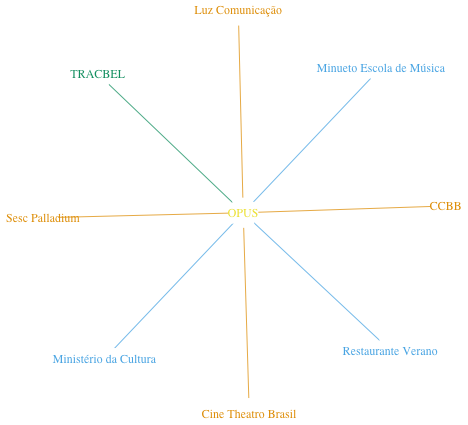
\includegraphics[scale=.7]{rede_opus.png}
		\fonte{Elaboração do autor usando linguagem \textbf{R} e \textbf{igraph} \cite{rlanguage,igraph}}
	\end{figure}
	
	\subsection{Diferenciação}
	
	De acordo com o dirigente entrevistado, a Orquestra OPUS procurou encontrar o seu papel, a sua identidade, no mercado das orquestras em Belo Horizonte buscando oferecer ao público algo diferente do que já existe e levando em conta a bagagem artística de seu maestro titular. ``A Filarmônica normalmente privilegia repertório romântico. A Sinfônica faz as temporadas de ópera na cidade. A OPUS seguiu para um lado mais popular'' (\textit{dirigente entrevistado}). O maestro da orquestra possui anos de experiência com música popular escrevendo arranjos, gravando e tocando. Esse experiência também se reflete na posição que a orquestra buscou para si na estrutura do mercado.
	
	
	\section{Orquestra Ouro Preto}\label{cap:ouropreto}
	
	A Orquestra Ouro Preto nasceu no ano 2000 fundada por Rufo Herrera e Ronaldo Toffolo com o nome de ``Orquestra Experimental da UFOP''. Hoje a orquestra possui cerca de 20 músicos mas seu tamanho pode variar de acordo com o repertório a ser executado. Normalmente, a orquestra privilegia repertório popular e repertório erudito para orquestra de cordas.
	
	A Orquestra Ouro Preto possui foca suas relações de parceria na iniciativa privada. De acordo com o dirigente entrevistado, ``100\% dos parceiros são da iniciativa privada. Não recebemos nenhum investimento direto do Estado. Até fugimos um pouco disso. A relação da orquestra com o Estado é sempre uma relação complicada. Há vários interesses que estão acima do interesse artístico'' (\textit{dirigente entrevistado}). É importante salientar que a orquestra obtém seu financiamento via leis de incentivo à cultura. Segundo o diretor entrevistado, a orquestra participa de uma modalidade da lei que provê um plano anual de manutenção da organização. Segundo o entrevistado, esse é o caso da Orquestra Ouro Preto, da Orquestra Sinfônica do Estado de São Paulo, do Museu de Arte Moderna do Rio de Janeiro, dentre outros corpos artísticos e espaços culturais do país. O projeto contempla a manutenção anual da organização e os patrocinadores investem já nesse planejamento.
	
	Para o entrevistado, trabalhar com a iniciativa privada dá maior liberdade de gestão do grupo embora tenha o ônus de fazer com que a orquestra esteja ``na maré do mercado'' (\textit{dirigente entrevistado}). É conhecido que a concorrência por financiamento é acirrada visto que a decisão da distribuição de investimento dos recursos das leis de incentivo à cultura fica a cargo das empresas. A orquestra, entretanto, possui estratégias bem delimitadas para competir e argumentar com os financiadores. Esse ponto será abordado oportunamente.
	
	\subsection{Estrutura e Financiamento}
	
	A Orquestra Ouro Preto possui um coordenador geral e um diretor artístico que estão no topo do processo decisório e gestão da organização. Além desses dois cargos centrais, há também a Coordenação de Criação, o Gerente, o Consultor Executivo (posição ocupada por uma empresa), a Gerência de Marca, a Coordenação de Comunicação, a Gestão Financeira, a Produção Executiva, a Assessoria de Produção, a Direção de Cena, o Conselho Consultivo e o Conselho Diretor\footnote{\url{http://www.orquestraouropreto.com.br/site/a-orquestra/}}. Entretanto, de acordo com o dirigente entrevistado, as relações entre as coordenações e demais órgãos na orquestra é bastante horizontal. ``As outras coordenações existem para fazer a parte artística funcionar. É um sistema bem diferente do que você vai encontrar em outras orquestras profissionais no país'' (\textit{dirigente entrevistado}). 
	
	O orçamento anual da orquestra gira entre dois e três milhões por ano. Ele depende muito do interesse de cada patrocinador. Desse montante, cerca de 40\% é destinado à folha de pagamento dos músicos, 20\% ao pagamento do pessoal administrativo e os outros 40\% destinados a custos de logística, viagens, etc.
	
	\subsection{Locais e ingressos}
	
	A orquestra possui uma série de concertos intitulada ``Domingos Clássicos'' que acontece aos domingos no Grande Teatro do Sesc Palladium. Os ingressos para esses concertos são comercializados numa média de 20 reais. Os concertos da turnê nacional acontecem sempre a preços populares. O entrevistado citou como exemplo um concerto realizado no Teatro Municipal de São Paulo em 2017 cujos ingressos foram comercializados a 40 reais e o balcão\footnote{Parte superior traseira do público nos teatros.} a 10 reais. Já as apresentações da turnê estadual são realizadas sempre em locais públicos e são gratuitas.
	
	\subsection{A rede da orquestra}
	
	A rede citada pelo dirigente entrevistado possui apenas relações de patrocínio e uma relação de parceria com o Sesc Palladium, espaço cultural onde a Orquestra Ouro Preto é ``orquestra residente''. Apresentamos uma representação da rede da orquestra na Figura \ref{rede-ouropreto}.
	
	\begin{figure}[!ht]
		\centering
		\caption{Rede Egocentrada da Orquestra Ouro Preto}
		\label{rede-ouropreto}
		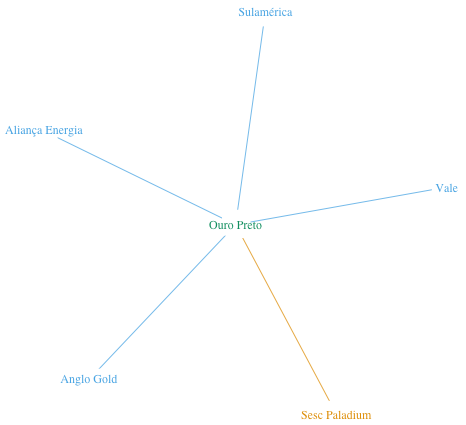
\includegraphics[scale=.7]{rede_ouropreto.png}
		\fonte{Elaboração do autor usando linguagem \textbf{R} e \textbf{igraph} \cite{rlanguage,igraph}}
	\end{figure}
	
	
	\subsection{Motivação}
	
	A Orquestra Ouro Preto sempre convida os músicos que irão fazer parte dela. Nesse sentido, a organização procura desenvolver uma relação muito próxima com esses músicos. O que a organização mais presta atenção no processo de escolha dos músicos não é a seleção em si mas uma espécie de período probatório onde cabe a decisão de mantê-lo ou não. Para o dirigente entrevistado, ``é crucial, para manter um músico na equipe, ver como ele funciona em grupo, como ele se relaciona, se ele é do tipo agregador ou desagregador, se causa problemas... Na orquestra nós soubemos manter pessoas no grupo com um grau de interesse muito grande pelo projeto'' (\textit{dirigente entrevistado}).
	
	``Tentamos motivar os músicos dando a eles a oportunidade de fazer coisas diferentes. Desse modo eles podem sair da `bolha' do repertório orquestral convencional'' (\textit{dirigente entrevistado}). 
	
	
	\subsection{Repertório e Branding}
	
	Segundo o entrevistado, a organização tem como uma de suas principais diretrizes a criação de uma identidade forte no mercado, a criação de uma marca. ``A orquestra é uma realidade completamente diferente de todas as outras. É uma orquestra independente, privada, que funciona a partir de projetos específicos e com um nome que carrega há 19 anos'' (\textit{dirigente entrevistado}).

	De acordo com o dirigente entrevistado, a orquestra sempre se engajou bastante na formação de público. Para ele, a orquestra representa o ``novo'', o que seria muito raro no planejamento cotidiano das orquestras em geral. Nesse sentido, a Orquestra Ouro Preto tenta resgatar o ``conceito moderno de orquestra'', a orquestra que produz projetos novos, atuais, com música de seu tempo, original e que dialogue com o público para que ele volte a sua atenção e comece a consumir os produtos da orquestra. ``A orquestra tem que competir com a TV, com a gasolina a 5 reais, com um sistema de transporte público ruim... Não pode ser 'vou tocar Bach porque Bach é importante'. Tem que ser mais do que isso...'' (\textit{dirigente entrevistado}). Desse modo, os produtos desenvolvidos pela Orquestra Ouro Preto são comissionados especialmente para a organização. A orquestra possui em seu repertório, projetos que são exclusivos. Um dos maiores custos da organização está relacionado com a comissão de composições e arranjos originais. 

	\begin{citacao}
		Hoje, somos a orquestra no Brasil que mais faz comissão de obras para compositores e arranjadores. Isso dá um caráter exclusivo ao que fazemos e nos diferencia no mercado. Se você quiser ouvir a nona sinfonia de Beethoven, você pode escolher com qual orquestra vai querer ouvir, com qual maestro...
		Se for uma obra de Mozart ou de Bach, pode ainda escolher qual estilo interpretativo... Mas se você quiser ouvir as ``Valencianas'', só vai ouvir com a Orquestra Ouro Preto. Se quiser ouvir ``O Pequeno Príncipe'', só vai ouvir com a Orquestra Ouro Preto. (\textit{dirigente entrevistado})
	\end{citacao}

	É possível verificar no site da orquestra alguns de seus CD's e DVD's provenientes desses projetos originais comentados acima. ``O Pequeno Príncipe'' é uma adaptação do maestro titular do clássico de Antoine de Saint-Exupéry com música do compositor Tim Rescala. Trata-se de uma composição para narrador e orquestra realizada com teatro de bonecos. Os produtos ``The Beatles'' e ``Valencianas'' são arranjos de autoria do arranjador e violinista Mateus Freire para canções do quarteto de Liverpool e do artista brasileiro Alceu Valença, respectivamente. A primeira foi realizada com a orquestra tocando junto a uma banda de rock. A segunda foi realizada junto ao artista autor das canções. O projeto ``Latinidade'' traz composições originais de autores latino-americanos. É comum a orquestra realizar concertos que privilegiem a integração de linguagens artísticas como música e teatro, música e cinema, etc. Seus concertos parecem possuir um caráter de espetáculo, de entretenimento para o público.

	``A orquestra possui a coisa mais importante para um artista hoje: casa cheia'' (\textit{dirigente entrevistado}). O entrevistado argumenta que a orquestra consegue atingir um público mais abrangente do que as demais concorrentes. ``Nós temos uma média de visualizações de vídeos no YouTube muito superior à da Filarmônica ou da própria OSESP. A OSESP é considerada a melhor orquestra do país e nós temos mais do dobro de ouvintes mensais no Spotify do que ela. Como podemos, então, definir o que é melhor?'' (\textit{dirigente entrevistado}). Os números da orquestra nas plataformas de \textit{streaming} são um dos principais pontos de argumentação junto às empresas para as quais eles apresentam possibilidade de parceria e costumam ter um peso muito grande na decisão de patrocinar. De acordo com o entrevistado, a preocupação com a aproximação e com a abrangência do público são diferenciais da organização. ``Já acatamos sugestões do público de arranjos, de repertório e fizemos. Tem um diálogo muito bom'' (\textit{dirigente entrevistado}). Para ele, as leis de incentivo à cultura tiveram um efeito colateral perverso na relação artista e público: ``Antes das leis, os artistas competiam pelo público. Agora eles competem pelo patrocínio. Isso é péssimo. Daí, você tem artistas com 1 milhão na conta e teatro vazio'' (\textit{dirigente entrevistado}).
	
	Muito embora a Orquestra Ouro Preto não seja considerada a orquestra de maior qualidade entre os entrevistados deste trabalho, ela se coloca, nas declarações de seu dirigente entrevistado, como uma organização diferenciada com um público diferenciado e com uma identidade de marca muito forte. Seu caráter exclusivo (devido aos produtos e repertório originais) e seus números grandes nas plataformas de \textit{streaming} são indicadores muito valorizados no cenário da música \textit{pop} e na indústria fonográfica, não necessariamente no mercado das orquestras. Essa preocupação proposital não era um achado esperado e coloca algumas questões muito interessantes sobre a qualidade nesse mercado específico que serão abordadas oportunamente.
	
	A seguir, apresentaremos os dados coletados junto aos músicos entrevistados na cidade de Belo Horizonte e as redes construídas a partir desses dados e das entrevistas com os dirigentes das orquestras.
	
	
	
	\chapter{Análise das Redes}
	
	\section{As redes entre músicos observadas}
	
	%a carga enorme de trabalho que os músicos da cidade possuem tanto de ensaios nas orquestras quanto de estudos fora de seu horário regular de trabalho (especialmente em se tratando de repertório cuja execução é tecnicamente mais desafiadora) e ao perfil característico dos músicos que, no contexto investigado, tendem a possuir alto status sócio-ocupacional e, em geral, selecionam de forma bastante criteriosa os compromissos nos quais irão se engajar.
	
	Os músicos de orquestra da cidade de Belo Horizonte não são um público de fácil acesso. Além de possuírem uma rotina bastante pesada de ensaios, estudo individual do repertório e aulas (sejam particulares ou nas universidades e escolas de música), eles contam com um status socioeconômico elevado o que faz com eles tenham uma seleção muito criteriosa dos compromissos que assumem. Contudo, a rede identificada a partir dos entrevistados parece ser bastante representativa do cenário musical orquestral de Belo Horizonte visto que, além das entrevistas em si, fizemos um trabalho de identificação do pertencimento de cada indivíduo citado na estrutura com as orquestras existentes.
	
	Foram usados quatro geradores de nomes\footnote{cf. Capítulo \ref{sec:geradores_nomes}.} para construir as redes de Aconselhamento, Amizade, Indicação para trabalho e Convites para tocar apresentadas na Figura \ref{redes-entre-musicos}. 	Todas exceto a rede de amizede foram aglutinadas para formar uma rede multiplexo de prestígio dos músicos. A rede multiplexo de prestígio está apresentada na Figura \ref{rede-multiplexo}.
	
	\begin{figure}[!ht]
		\centering
		\caption{Redes entre músicos}
		\label{redes-entre-musicos}
		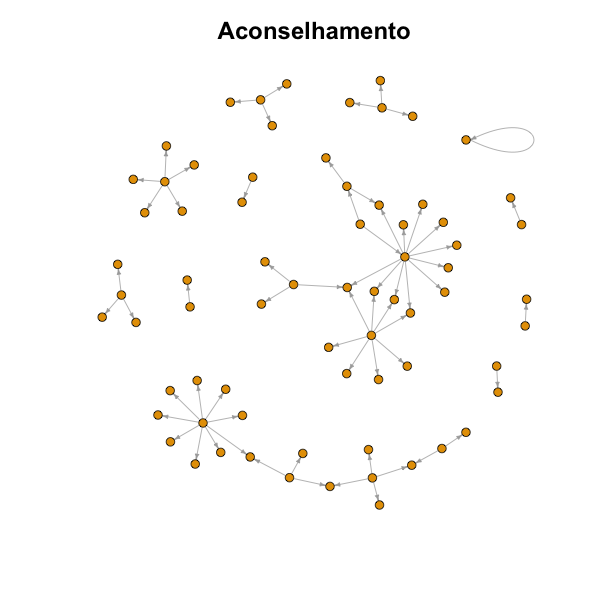
\includegraphics[scale=.35]{rede_conselho.png}
		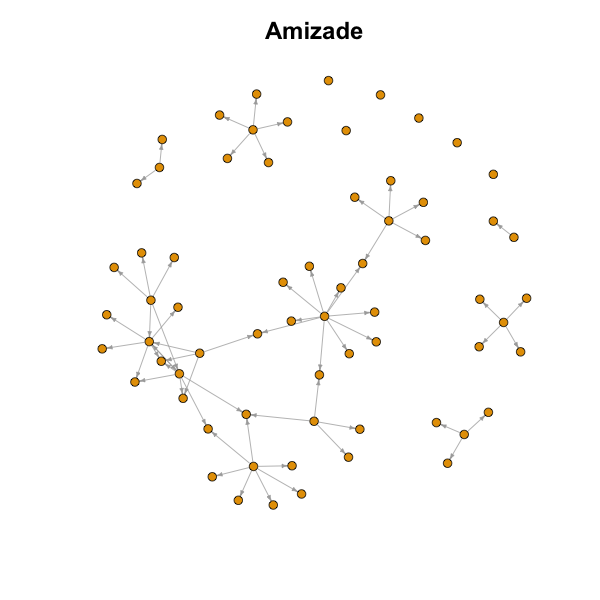
\includegraphics[scale=.35]{rede_amizade.png}
		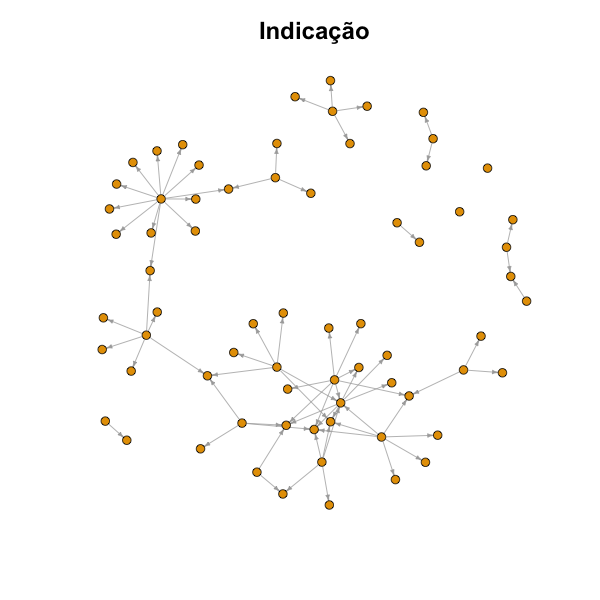
\includegraphics[scale=.35]{rede_indicacao.png}
		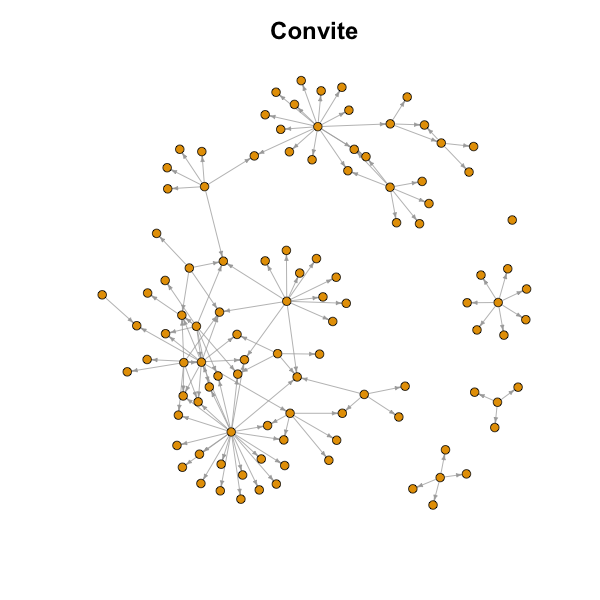
\includegraphics[scale=.35]{rede_convite.png}
		\fonte{Elaboração do autor usando linguagem \textbf{R} e \textbf{igraph} \cite{rlanguage,igraph}}
	\end{figure}
	

	\begin{figure}[!ht]
		\centering
		\caption{Rede multiplexo de prestígio entre músicos}
		\label{rede-multiplexo}
		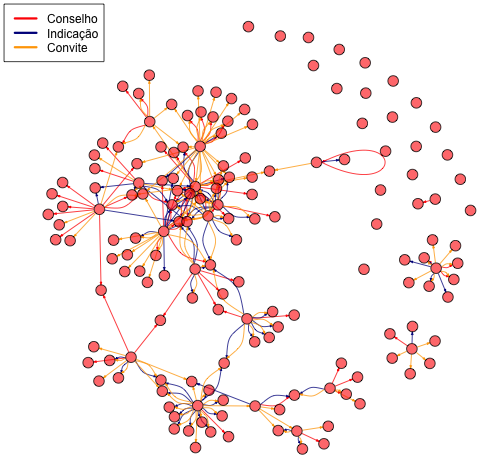
\includegraphics[scale=.7]{rede_multiplexo.png}
		\fonte{Elaboração do autor usando linguagem \textbf{R} e \textbf{igraph} \cite{rlanguage,igraph}}
	\end{figure}



	Ao todo 19 músicos colaboraram com a pesquisa. Dessas respostas foi possível elaborar uma rede multiplexo com 161 indivíduos. Esses indivíduos estão associados a 24 organizações identificadas. A tabela \ref{redes-descritivas1} apresenta algumas medidas descritivas das redes identificadas.

	% latex table generated in R 3.5.1 by xtable 1.8-3 package
	% Wed Jan  9 11:24:52 2019
	\begin{table}[!ht]
		\ibgetab{
		\centering
		\label{redes-descritivas1}
		\caption{Medidas descritivas das redes de indivíduos}
	}
		{\begin{tabular}{rllllp{1.5cm}p{1.5cm}}
			\hline
			\textbf{Rede} & \textbf{N} & \textbf{Laços} & \textbf{Densidade} & \textbf{Diâmetro} & \textbf{Distância média} & \textbf{Grau médio}  \\ 
			\hline
			Aconselhamento & 71 & 64 & 0.0129 & 2 & 1.1600 & 0.9014 \\ 
			Amizade & 66 & 62 & 0.0145 & 3 & 1.2771 & 0.9394  \\ 
			Indicação & 69 & 73 & 0.0156 & 2 & 1.1798 & 1.0580 \\ 
			Convite & 106 & 127 & 0.0114 & 3 & 1.3450 & 1.1981 \\  
			Multiplexo - Prestígio & 161 & 264 & 0.0102 & 3 & 1.4549 & 1.6398 \\
			\hline
		\end{tabular}
	}
	{\fonte{Elaboração do autor.}}
	\end{table}


	Entre as redes observadas, é possível perceber que a rede de convites para se apresentar em conjunto foi a que gerou mais nós e laços. As demais geraram redes de tamanhos similares. Todas possuem baixa densidade (devido ao número pequeno de respondentes), possuem diâmetros 2 e 3, distância média e grau médio próximos de 1. No Anexo 4 apresentamos as medidas de centralidade de grau, centralidade de intermediação, centralidade de proximidade e constraint para as 4 redes observadas e para a rede multiplexo de prestígio (cf Tabelas \ref{centralidades:conselho}, \ref{centralidades:amizade}, \ref{centralidades:indicacao}, \ref{centralidades:convite} e \ref{centralidades:multiplexo}).
	
	Os indivíduos que possuem os maiores índices de centralidade de grau e centralidade de intermediação estão concentrados, respectivamente, na Orquestra Filarmônica de MG, na Orquestra Ouro Preto e na Orquestra SESIMINAS. Um músico do naipe de percussão aparece como um dos nós mais centrais em todas as redes mapeadas. Outro músico também percussionista, três músicos do naipe das madeiras\footnote{Tracidionalmente o naipe composto por flautas, oboés, clarinetes e fagotes.} e um músico do naipe das cordas.
	
	Várias tentativas de blockmodel foram realizadas. Entretanto, este modelo não apresentou resultados relevantes. Ele foi capaz de separar os nós que responderam ao questionário e os que foram identificados mas não responderam.

	
	Investigamos ainda a correlação entre as redes utilizando a técnica da correlação QAP\footnote{A correlação QAP {Quadratic Assignment Procedure} é calculada empilhando as colunas das matrizes para formar vetores e calculando uma medida escolhida de correlação (neste caso, o $r$ de Pearson). O teste de hipótese é feito através de permutações das matrizes, ou seja, as linhas e colunas são rearranjadas aleatoriamente para testar a proporção em que todos os resultados com matrizes permutadas resultam numa correlação tão grande quanto a observada \cite{borgatti2018analyzing}.} Os resultados estão apresentados na Tabela \ref{cor:redes}. Todas as corelações giram em torno de 0,2 com exceção da correlação entre indicações para trabalho e convite para tocar: $r = 0,538$, indicando uma correlação mais forte.
	
	% latex table generated in R 3.5.1 by xtable 1.8-3 package
	% Fri Jan 11 13:07:07 2019
	\begin{table}[ht]
		\ibgetab{
		\centering
		\caption{Matriz de correlações QAP entre as redes observadas}
		\label{cor:redes}
	}
		{\begin{tabular}{rrrrr}
			\hline
			& Aconselhamento & Amizade & Indicação & Convite \\ 
			\hline
			Aconselhamento & 1.000 &  &  &  \\ 
			Amizade & 0.206 & 1.000 &  &  \\ 
			Indicação & 0.204 & 0.176 & 1.000 &  \\ 
			Convite & 0.232 & 0.166 & 0.538 & 1.000 \\ 
			\hline
		\end{tabular}
	}
		{\fonte{Elaboração do autor.}}
	\end{table}
	
	
	\section{A rede multinível}
	
	Após a construção da rede interganizacional, a construção das redes entre indivíduos e a identificação dos laços de afiliações dos indivíduos mencionados a organizações, elaboramos a rede multinível apresentada na Figura \ref{rede-multinivel}.
	
	
	\begin{figure}[!ht]
		\centering
		\caption{Rede Multinível}
		\label{rede-multinivel}
		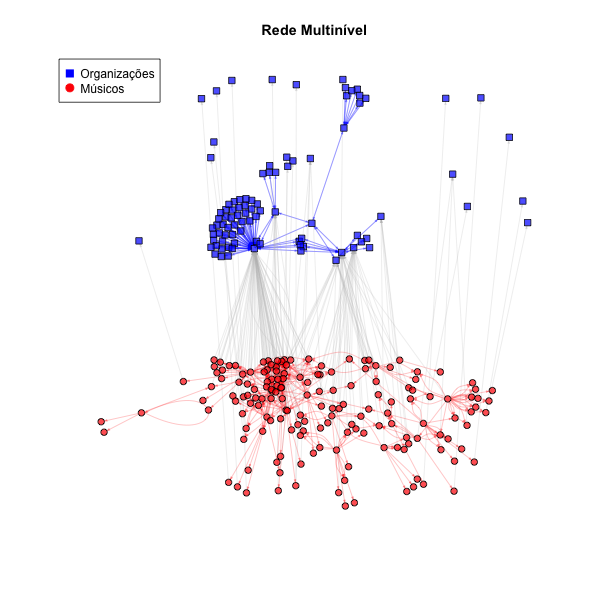
\includegraphics[scale=.7]{rede_multinivel.png}
		\fonte{Elaboração do autor usando linguagem \textbf{R} e \textbf{multinets} \cite{rlanguage,multinets}}
	\end{figure}
	
	O grafo representa em azul as organizações identificadas e, também em azul, os laços entre elas, em vermelho os músicos identificados e os laços entre eles (aqui todas as quatro redes observadas foram agrupadas formando um multiplexo) e em cinza, os laços de afiliação entre músicos e organizações. Por razões técnicas\footnote{Tradicionalmente, as redes \textit{2-mode} contém laços de afiliações que são essencialmente não direcionados. Não há como um indivíduo trabalhar numa organização e essa organização não tê-lo contratado. Contudo, as redes entre indivíduos e organizações são redes direcionadas. O pacote \textbf{igraph} não permite que numa mesma rede hajam laços direcionados e não direcionados o que, na verdade, não faz sentido pois as redes são representações de uma relação apenas entre nós.}, os laços de afiliação (tradicionalmente não direcionados) foram representados como laços direcionados mútuos. A rede multinível possui densidade $\delta = 0,0097$, diâmetro 5 e distância geodésica média 2,74. Conforme exposto no capítulo \ref{cap:multinivel}, procederemos com as análises de ambos os níveis em separado bem como das transformações das afiliações.
	
	
	\subsection{O nível dos músicos}
	
	Estimamos um ERGM para explicar os laços que compõem a rede multiplexo de prestígio. Assim procedemos pois não estamos interessados em explicar, necessariamente, os convites ou indicações para trabalho de forma efetiva mas o reconhecimento de uma grande capacidade técnica/musical mensurada pelos laços observados. O modelo explica, portanto, a emergência de uma estrutura de reconhecimento de uma certa autoridade artística.
	
	
	
	\begin{table}[!ht]
		\ibgetab{
		\centering
		\caption{ERGM - rede multiplexo de prestígio}
		\label{ergm:prestigio-coefs}
	}
			{\begin{tabular}{p{6cm} c c }
				\hline
				 &  & ERGM results \\
				\hline
                           Edges           &	 \raisebox{-.5\height}{
\includegraphics[scale=.5]{arc.png}}
                                               & $-6.11 \; (0.33)^{***}$ \\
                           Geometrically weighted edgewise shared partner distribution           & \raisebox{-.5\height}{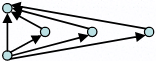
\includegraphics[scale=.5]{gwesp.png}}    & $2.23 \; (0.23)^{***}$  \\
				Geometrically weighted edgewise shared partner distribution: decay     &		& $-0.02 \; (0.44)$       \\
				Geometrically weighted in-degree distribution     & \raisebox{-.5\height}{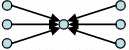
\includegraphics[scale=.5]{gwidegree.png}}   & $3.33 \; (0.40)^{***}$  \\
				Geometrically weighted in-degree distribution: decay & 	& $-0.20 \; (0.09)^{*}$   \\
				2-Paths    & \raisebox{-.5\height}{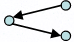
\includegraphics[scale=.5]{2paths.png}}      	& $-0.88 \; (0.11)^{***}$ \\
				Homophily (Sexo)  & \raisebox{-.5\height}{
\includegraphics[scale=.5]{homophily.png}}	& $0.47 \; (0.22)^{*}$    \\
				Attribute (Prestígio da Orquestra) & \raisebox{-.5\height}{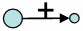
\includegraphics[scale=.5]{attribute_sum.png}} & $0.20 \; (0.02)^{***}$  \\
				Covariate Network (Amizade) & \raisebox{-.5\height}{
\includegraphics[scale=.5]{covariate.png}}   & $3.09 \; (0.26)^{***}$  \\
				\hline
				AIC      &       & 1663.29                 \\
				BIC        &     & 1726.19                 \\
				Log Likelihood & & -823.65                 \\
				\hline
				\multicolumn{3}{l}{\scriptsize{$^{***}p<0.001$, $^{**}p<0.01$, $^*p<0.05$}}
			\end{tabular}
		}
		{\fonte{Elaboração do autor usando \textbf{statnet} \cite{ergm,hunter2008ergm}}}
	\end{table}
	
	
	O primeiro parâmetro (\textit{Edges}) estima a quantidade de laços na rede. O valor negativo do parâmetro indica que na rede investigada os laços não estão restritos ao nível diádico mas sim ``encaixotados'' em microestruturas da tríade ou para além da tríade. Dito de outra forma, na rede em questão não há uma tendência de formação de díades isoladas umas das outras. O parâmetro \textit{Geometrically weighted edgewise shared partner distribution} estima o surgimento de triangulações de ordem superior (\textit{higher order}), ou seja, a distribuição de quantidades de nós que fazem o fechamento de triângulos para a base (\textit{i, j}). Trata-se do efeito \textit{closure}, ou fechamento das redes \cite{robins2007introduction}. O seu resultado positivo indica a tendência de buracos estruturais se fecharem quando há múltiplos caminhos independentes entre \textit{i} e \textit{j}. Dito de outra forma, pudemos identificar um efeito de fechamento, uma tendência à triangulação quanto maior o número de nós compartilhados entre dois nós (\textit{i, j}). O parâmetro de fechamento \textit{decay} não significativo mostra que a tendência se mantém constante em toda a distribuição (isso faz sentido visto que foram estimados os fechamentos múltiplos apenas até $k = 2$). Já o parâmetro \textit{geometrically weighted in-degree distribution} estima um efeito de concentração de laços recebidos por alguns nós. O parâmetro positivo indica que os laços de entrada, ou seja, os ``reconhecimentos de autoridade musical'' não são distribuídos igualmente pela rede mas, ao contrário, tendem a uma grande concentração. O parâmetro de caída associado a essa estatística negativo e significativo mostra que quanto maior o número de laços de entrada, menor tende a ser a caída do efeito, ou seja, maior ainda a concentração. O parâmetro \textit{2-Paths}, ou seja, a construção de tríades do tipo 021C e 111U\footnote{cf. Figura \ref{triades-man}.}, caminhos de 2 passos literalmente, obteve resultado negativo e significativo. Esse resultado também mostra a não igualdade da distribuição de laços, reforçando a constatação de alta concentração.
	
	No modelo foram testados 3 parâmetros exógenos, a saber, homofilia com relação ao sexo, o atributo ``prestígio da orquestra'' e a rede de amizade observada. O modelo indica uma leve tendência à homofilia por sexo, ou seja, os músicos tendem a reconhecer pessoas do mesmo sexo como autoridades musicais. Esse resultado, entretanto, não diz muito a respeito da estrutura, visto que a grande maioria dos indivíduos identificados é homem (82,5\%).	O atributo ``prestígio da orquestra'' foi construído a partir da classificação feita pelos respondentes. À orquestra considerada a de melhor qualidade pelo maior número de respondentes foi atribuído o valor de 5 e à orquestra considerada a de menor qualidade foi atribuída o valor de 1 e somados os valores para cada músico (pois alguns músicos tocam em mais de uma orquestra). O parâmetro positivo e significante mostra uma leve tendência de que indivíduos participantes em orquestras mais prestigiosas tendam formar laços com músicos de orquestras igualmente prestigiosas, ou seja, a atribuir prestígio a seus pares. Exatamente, o parâmetro diz que quanto maior a soma dos valores de prestígio da orquestra dos nós (\textit{i, j}), maior a probabilidade da existência do laço. Por fim, os laços de amizade tem um efeito positivo sobre o reconhecimento de competência musical. Há maiores chances de reconhecimento de competência entre amigos do que entre pessoas que não possuem laço de amizade.
	
	Em linhas gerais, o modelo aponta para uma grande tendência de concentração do prestígio em poucos indivíduos. Essa concentração é explicada mais pelas relações de amizade do que pelo sexo do indivíduo ou pela qualidade percebida da orquestra onde ele atua. O modelo teve um excelente ajuste. Os gráficos de avaliação de ajuste (\textit{goodness of fit}) na Figura \ref{gof:prestigio} mostram a adequação das redes simuladas aos dados observados. Em regras gerais a avaliação dos gráficos segue a seguinte lógica: A linha escura dos dados observados deve estar contida dentro das caixas que mostram a distribuição dos parâmetros estimados nas simulações. Se não estiver, isso significa que o modelo simulou redes que não se assemelham à rede observada e, portanto, os parâmetros possuem viés.
	
	
	\begin{figure}[!ht]
		\centering
		\caption{Gráficos de ajuste do modelo ERGM para a rede multiplexo de prestígio}
		\label{gof:prestigio}
		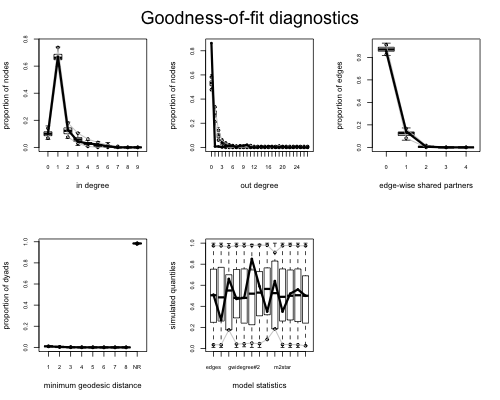
\includegraphics[scale=.8]{gof_individuos.png}
		\fonte{Elaboração do autor usando \textbf{statnet} \cite{ergm,hunter2008ergm}}
	\end{figure}
	
	Vamos agora investigar o nível individual a partir do nível meso da rede, ou seja, dos laços de afiliação de músicos a organizações. A partir da filtragem desses laços e sua transformação de uma rede \textit{2-mode} para uma rede \textit{1-mode} obtemos uma relação de coparticipação de atores nas mesmas organizações\footnote{Essa transformação, conforme argumentamos na seção \ref{cap:multinivel}, pressupõe que indivíduos afiliados às mesmas organizações constroem relações lá dentro. Há várias críticas a essa transformação, muito embora, na análise das redes multinível, ela seja recomendada por \citeonline{brailly2016market}.}. O componente principal da rede (foram retirados os nós isolados e outros subgrupos pequenos) está representado na Figura \ref{rede:coparticipacao} onde o tamanho do vértice indica a centralidade de intermediação. Sua análise visual já demonstra que há um nó absolutamente central na estrutura pois já teve passagens por quatro das cinco orquestras investigadas em Belo Horizonte. Há também outros 5 nós na parte de baixo do grafo que fazem intermediação entre duas regiões do grafo e um na parte de cima. Curioso notar que esse nó que aparece no centro do grafo não obteve grande relevância posicional nas outras redes mensuradas mas possui posicionamento privilegiado na participação de organizações.
	
	
	\begin{figure}[!ht]
		\centering
		\caption{Rede intermúsicos por coparticipação em organizações (transformação 2-mode para 1-mode) -- componente principal}
		\label{rede:coparticipacao}
		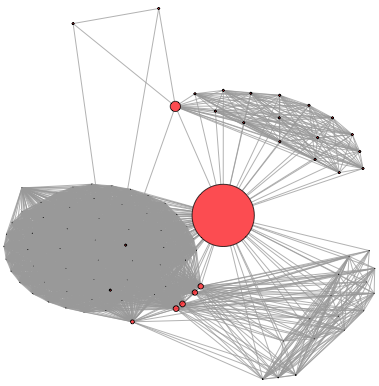
\includegraphics[scale=.7]{mesonivel1.png}
		\fonte{Elaboração do autor.}
	\end{figure}
	
	%Para entender a articulação da estrutura, estimamos um blockmodel estocástico e um blockmodel bayesiano segundo os desenvolvimentos de \citeonline{daudin2008mixture} e \citeonline{latouche2012variational}. O blockmodel estocástico variacional obteve o melhor desempenho. O modelo indicou que a divisão da rede em 3 subgrupos obteve o melhor critério de ajuste (ICL). Os resultados da estimação e uma representação da matriz reordenada estão apresentados na Figura \ref{block_ind_res}. O componente principal da rede multiplexo de prestígio com os blocos demarcados está apresentado na Figura \ref{rede_prestigio_blocos}.
	
	
	
%	\begin{figure}[!ht]
%		\centering
%		\caption{Resultados do blockmodel estocástico}
%		\label{block_ind_res}
%		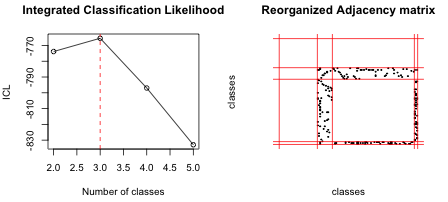
\includegraphics[scale=.8]{sbm_individual_out.png}
%		\fonte{Elaboração do autor usando pacote \textbf{mixer} \cite{daudin2008mixture}.}
%	\end{figure}


%	\begin{figure}[!ht]
%		\centering
%		\caption{Rede Multiplexo de prestígio com blocos}
%		\label{rede_prestigio_blocos}
%		%\includegraphics[scale=.7]{}
%		\fonte{Elaboração do autor usando pacote \textbf{mixer} \cite{daudin2008mixture}.}
%	\end{figure}
		
		
	\subsection{O nível organizacional}
	
	Adotaremos a mesma estratégia para investigar a rede entre organizações. O componente principal da rede observada entre organizações está representada na Figura \ref{rede:organizacoes}. O tamanho do nó indica a centralidade de grau.
	
	
	\begin{figure}[ht]
		\centering
		\caption{Rede observada entre organizações -- componente principal}
		\label{rede:organizacoes}
		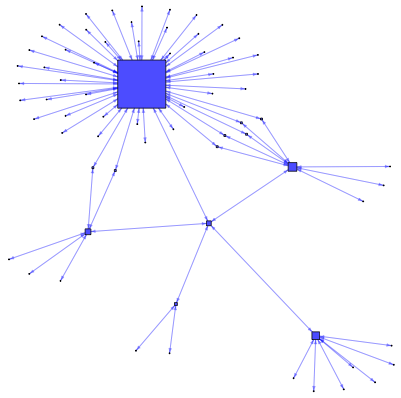
\includegraphics[scale=.7]{nivel2.png}
		\fonte{Elaboração do autor.}
	\end{figure}
	
	A complexidade das orquestras já foi discutida nos capítulos \ref{cap:filarmonica} a \ref{cap:ouropreto}. Aqui é possível visualizar de maneira mais completa, a complexidade das orquestras. O ponto central conectando toda a estrutura é o Ministério da Cultura (pequeno ponto localizado exatamente no meio do grafo da figura \ref{rede:organizacoes}). Ele configura o que chamamos de \textit{cutpoint}, ou seja, se ele fosse retirado, a estrutura se fragmentaria. A visualização mostra a centralidade da Lei Rouanet para o funcionamento da música de orquestra em Belo Horizonte. É possível perceber também alguns nós fazendo conexão entre as orquestras (5 nós na parte superior direta e 2 nós à esquerda). Trata-se de empresas que patrocinam as orquestras em Belo Horizonte e teatros, locais de apresentação. A estrutura reconstruída a partir das afiliações também possui uma configuração muito interessante. A representação de seu componente principal está na Figura \ref{rede:mesonivel2}.
	
	\begin{figure}[!ht]
		\centering
		\caption{Rede interorganizacional a partir da cofiliação de músicos (transformação 2-mode para 1-mode) -- componente principal}
		\label{rede:mesonivel2}
		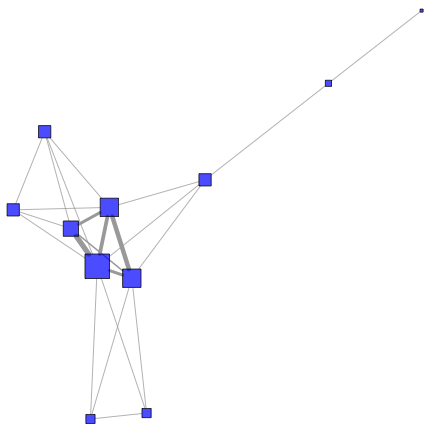
\includegraphics[scale=.7]{mesonivel2.png}
		\fonte{Elaboração do autor.}
	\end{figure}

	O tamanho dos vértices na Figura \ref{rede:mesonivel2} representa a centralidade de grau. É possível perceber um núcleo fortemente conectado no centro do grafo composto pelas orquestras de Belo Horizonte exceto a OPUS. Os nós tangenciais na parte superior à esquerda e inferior do grafo são outras orquestras da qual os músicos já fizeram parte e que, por esse motivo, carregam conhecimento e cultura desses lugares para as organizações que estão no centro. Os nós na ponta superior direta são instituições de ensino superior e uma escola de música da cidade. É possível perceber aqui a estreita ligação que o mercado das orquestras tem com as universidades.
	
	\subsubsection{Blockmodels}
	
	Estimamos dois modelos de blocos para identificar subgrupos na estrutura gerada pelo compartilhamento de colaboradores (Figura \ref{sbmout:mesonivel2}). e na estrutura observada a partir das entrevistas com os dirigentes (Figura \ref{sbmout:orgs}). Em ambos os casos, tanto o modelo ``variacional'' quanto o modelo bayesiano produziram resultados idênticos. No primeiro caso, na rede de compartilhamento de colaboradores, o modelo identificou dois blocos de nós estruturalmente equivalentes (Figura \ref{blocos:mesonivel2}).
	
	
	\begin{figure}[!ht]
		\centering
		\caption{Blockmodel para rede de organizações a partir das afiliações}
		\label{sbmout:mesonivel2}
		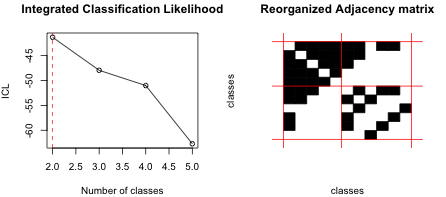
\includegraphics[scale=.8]{blockmesonivel2.png}
		\fonte{Elaboração do autor usando o pacote \textbf{mixer} \cite{daudin2008mixture,latouche2012variational}}
	\end{figure}

	\begin{figure}[!ht]
		\centering
		\caption{Blockmodel para rede de organizações observada}
		\label{sbmout:orgs}
		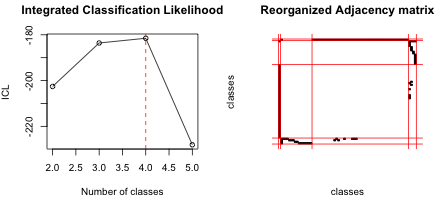
\includegraphics[scale=.8]{blockoutorgs.png}
		\fonte{Elaboração do autor usando o pacote \textbf{mixer} \cite{daudin2008mixture,latouche2012variational}}
	\end{figure}

	\begin{figure}[!ht]
		\centering
		\caption{Rede interorganizacional a partir da cofiliação de músicos (transformação 2-mode para 1-mode) com blocos de nós estruturalmente equivalentes}
		\label{blocos:mesonivel2}
		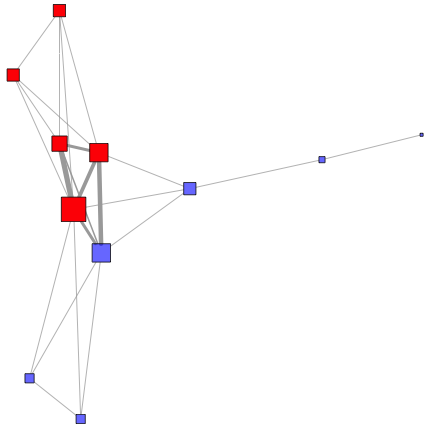
\includegraphics[scale=.7]{block_rede_mesonivel2.png}
		\fonte{Elaboração do autor.}
	\end{figure}
	
	
	É curioso notar que o modelo de blocos alocou num mesmo bloco as três orquestras que possuem o maior escore de qualidade percebida calculado e, no outro, alocou a orquestra que ocupa a quarta posição no ranking. A última orquestra não está presente nessa estrutura pois não houveram identificações de afiliação a ela nos dados.
	
	
	\begin{figure}[!ht]
		\centering
		\caption{Rede observada entre organizações com blocos de nós estruturalmente equivalentes}
		\label{blocos:orgs}
		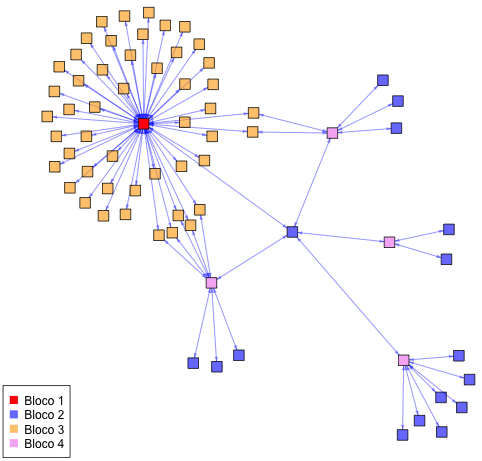
\includegraphics[scale=.7]{block_nivel2_observado.png}
		\fonte{Elaboração do autor.}
	\end{figure}

	Já o blockmodel da rede observada identificou quatro blocos de nós estruturalmente equivalentes (Figura \ref{blocos:orgs}). A orquestra Filarmônica ficou alocada sozinha no bloco 1, as demais orquestras no bloco 4. O bloco 3 é formado pelas organizações que possuem relacionamento com a Filarmônica e com outras duas orquestras (7 delas). O bloco 2 é formado pelas organizações que possuem relacionamento com as outras orquestras da cidade. Este modelo captou que a Filarmônica possui um perfil relacional diferenciado em relação às outras orquestras que, por sua vez, possuem perfil relacional semelhante.

        Ambos os modelos nos apresentam informações complementares sobre o nosso objeto de estudo embora, à primeira vista, pareçam contraditórios. Eles nos mostram que, com relação às relações interorganizacionais, a Filarmônica possui um perfil relacional único embora compartilhe músicos com outras duas orquestras que também possuem alta qualidade percebida. Uma explicação possível para este último resultado seria o fato de que vários componentes da orquestra considerada de melhor qualidade participam nas outras duas subsequentes no ranking. Isso faria com que o conhecimento qualitativo dos músicos compartilhados fosse aprendido por seus pares nas outras orquestras elevando a qualidade. Essa hipótese, contudo, só poderá ser verificada com trabalho qualitativo posterior.

	\begin{comment}
	%\subsubsection{ERGM}
	
	Por fim, estimamos um ERGM para investigar a emergência da estrutura entre organizações. Várias tentativas foram realizadas e os diversos modelos de circuitos sociais (\textit{higher order}) testados não convergiram. Foi estimado um modelo markoviano com dois parâmetros, a saber, \textit{Edges} (laços) e \textit{K-star(2)} (estrela de 2 pontas) (Tabela \ref{ergm:organizacoes}). O primeiro parâmetro indica que a rede possui menos laços do que o esperado se a estrutura fosse aleatória. O segundo parâmetro indica uma leve tendência à concentração de laços.
	
	\begin{table}[!ht]
		\ibgetab{
		\centering
		\caption{ERGM - rede entre organizações}
		\label{ergm:organizacoes}	
	}
			{\begin{tabular}{l c c }
				\hline
				 &  & ERGM - results \\
				\hline
				Edges & \raisebox{-.5\height}{
\includegraphics[scale=.5]{edges.png}}         & $-1.51 \; (0.67)^{*}$ \\
				K-star (2)  & \raisebox{-.5\height}{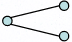
\includegraphics[scale=.5]{2star.png}}       & $0.16 \; (0.08)^{*}$  \\
				\hline
				AIC      &      & 77.75                 \\
				BIC        &    & 81.77                 \\
				Log Likelihood  &  & -36.88                \\
				\hline
				\multicolumn{3}{l}{\scriptsize{$^{***}p<0.001$, $^{**}p<0.01$, $^*p<0.05$}}
			\end{tabular}
	}
	{\fonte{Elaboração do autor usando \textbf{statnet}, \cite{ergm,hunter2008ergm}}}
	\end{table}
      \end{comment}
      
	
	\section{Testes de hipóteses}
	
	Para testar as hipóteses traçadas no capítulo \ref{hipoteses}, utilizaremos o \textit{Network Autocorrelation Model} conforme especificado na Equação \ref{NAM}. Visando um bom ajuste aos dados, estimamo um modelo linear generalizado com distribuição \textit{gamma} e link ``log''. Nosso modelo estimou a qualidade percebida de cada orquestra como função da rede observada entre organizações levando em consideração tanto as relações de um passo quanto de dois passos, da soma da centralidade dos músicos a ela afiliados (um parâmetro, neste caso, essencialmente multinível), do salário médio pago pela orquestra (em milhares de reais), do orçamento anual (em centenas de milhares de reais), da complexidade
	%, da proximidade com o estado 
	e da centralidade de grau.	
	Estatísticas descritivas das variáveis estão apresentadas na Tabela \ref{varsMAN}.
	
	% Table created by stargazer v.5.2.2 by Marek Hlavac, Harvard University. E-mail: hlavac at fas.harvard.edu
	% Date and time: Mon, Jan 14, 2019 - 11:50:22
	\begin{table}[!htbp] 
		\ibgetab{
		\centering 
		\caption{Estatísticas descritivas das variáveis do \textit{Network Autocorrelate Model}} 
		\label{varsMAN}
	}
		{\begin{tabular}{@{\extracolsep{5pt}}lcccccc} 
			\\[-1.8ex]\hline 
			\hline \\[-1.8ex] 
			Statistic &  \multicolumn{1}{c}{Mean} & \multicolumn{1}{c}{St. Dev.} & \multicolumn{1}{c}{Min} & \multicolumn{1}{c}{Pctl(25)} & \multicolumn{1}{c}{Pctl(75)} & \multicolumn{1}{c}{Max} \\ 
			\hline \\[-1.8ex] 
			Qualidade &  0.314 & 0.866 & 0.1 & 0.1 & 0.1 & 5.1 \\ 
			Rede interorganizacionais - Dist 1  & 4.543 & 2.563 & 0 & 4 & 5 & 15 \\ 
			Rede interorganizacionais - Dist 2  & 0.857 & 3.136 & 0 & 0 & 0 & 14 \\ 
			Centralidade de grau & 2.171 & 5.983 & 1 & 1 & 1 & 50 \\ 
			Centr. dos músicos (soma) & 2.929 & 16.859 & 0 & 0 & 0 & 137 \\ 
			Salário médio pago & 0.209 & 0.967 & 0 & 0 & 0 & 7 \\ 
			Orçamento anual & 0.518 & 3.576 & 0 & 0 & 0 & 30 \\ 
			Complexidade & 0.371 & 1.590 & 0 & 0 & 0 & 9 \\
			Prox. com o Estado & 0.214 & 0.866 & 0 & 0 & 0 & 5 \\ 
			\hline \\[-1.8ex] 
		\end{tabular}
	}
	{\fonte{Elaboração do autor.}}
	\end{table} 

	A variável \textit{Qualidade} foi construída a partir das respostas dos músicos ao questionário sociométrico online onde a orquestra identificada como a de melhor qualidade recebia 5 e a de menor qualidade recebia 1. Quando uma orquestra não era citada pelo respondente recebia o valor 0 (ausência de classificação). As demais organizações da rede receberam também 0. A essa variável foi somado 0,1 para tornar possível a estimação do modelo generalizado com distribuição \textit{gamma} e \textit{link log}. Como não possuímos dados das covariáveis para todas as organizações presentes na estrutura, apenas as orquestras, elaboraremos seis modelos; o primeiro com apenas as variáveis da estrutura relacional, ou seja, a rede e a centralidade de grau, e um modelo para cada covariável controlando pelas variáveis estruturais. Colocar as covariáveis juntas no modelo cria, desse modo, um viés.
	Os resultados dos modelos estimados estão apresentados na Tabela \ref{res:NAM} abaixo.
	
	
	\begin{table}[!ht]
		\ibgetab{
		\centering
		\caption{Network Autocorrelation Models - Resultados - Dependente: Qualidade percebida da orquestra}
		\label{res:NAM}
	}
		{\begin{tabular}{l c c c c c c }
			\hline
			 & Model 1 & Model 2 & Model 3 & Model 4 & Model 5 & Model 6 \\
			\hline
			(Intercept)                & $-2.29^{***}$ & $-2.28^{***}$ & $-2.29^{***}$ & $-2.27^{***}$ & $-2.29^{***}$ & $-2.30^{***}$ \\
			& $(0.05)$      & $(0.04)$      & $(0.02)$      & $(0.05)$      & $(0.05)$      & $(0.01)$      \\
			Rede interorg. - Dist 1           & $-0.01$       & $0.02^{*}$    & $0.01$        & $0.01$        & $-0.01$       & $0.00$        \\
			& $(0.01)$      & $(0.01)$      & $(0.00)$      & $(0.01)$      & $(0.01)$      & $(0.00)$      \\
			Rede interorg. - Dist 2          & $0.25^{***}$  & $0.25^{***}$  & $0.18^{***}$  & $0.28^{***}$  & $0.23^{***}$  & $0.14^{***}$  \\
			& $(0.01)$      & $(0.01)$      & $(0.01)$      & $(0.01)$      & $(0.01)$      & $(0.00)$      \\
			Cent. de grau                  & $0.03^{***}$  & $-0.10^{***}$ & $-0.05^{***}$ & $-0.08^{*}$   & $0.02^{***}$  & $-0.01^{***}$ \\
			& $(0.00)$      & $(0.01)$      & $(0.01)$      & $(0.03)$      & $(0.01)$      & $(0.00)$      \\
			Cent. músicos (soma) &               & $0.05^{***}$  &               &               &               &               \\
			&               & $(0.01)$      &               &               &               &               \\
			Salário médio pago         &               &               & $0.65^{***}$  &               &               &               \\
			&               &               & $(0.04)$      &               &               &               \\
			Orçamento        &               &               &               & $0.17^{**}$   &               &               \\
			&               &               &               & $(0.05)$      &               &               \\
			Complexidade     &               &               &               &               & $0.06^{*}$    &               \\
			&               &               &               &               & $(0.03)$      &               \\
			Prox. Estado      &               &               &               &               &               & $0.58^{***}$  \\
			&               &               &               &               &               & $(0.01)$      \\
			\hline
			AIC                        & -329.87       & -370.08       & -440.87       & -336.66       & -332.87       & -636.36       \\
			BIC                        & -318.63       & -356.59       & -427.38       & -323.17       & -319.38       & -622.86       \\
			Log Likelihood             & 169.94        & 191.04        & 226.44        & 174.33        & 172.44        & 324.18        \\
                   Deviance                   & 1.98          & 1.09          & 0.40          & 1.75          & 1.85          & 0.02          \\
                   Effron's Pseudo $R^2$ & 0.714 & 0.837 & 0.918 & 0.806 & 0.774 & 0.996 \\
			Num. obs.                  & 70            & 70            & 70            & 70            & 70            & 70            \\
			\hline
			\multicolumn{7}{l}{\scriptsize{$^{***}p<0.001$, $^{**}p<0.01$, $^*p<0.05$}}
		\end{tabular}
	}
	{	\fonte{Elaboração do autor usando o pacote \textbf{tnam} \cite{tnam}.} }
	\end{table}

	
	A partir do modelo 1, faremos as análises referentes às variáveis estruturais. A rede vizinha não obteve resultado estatisticamente significativo. Ao levar em conta os nós a dois passos de distância, entretanto, encontramos um efeito positivo e significativo. Esse efeito controla a atividade dos nós com os quais o ego não possui relação direta. A centralidade de grau obteve também um resultado positivo e significativo. Esses dois resultados em conjunto podem ser vistos como excelentes indicadores da complexidade da rede egocentrada de cada nó. Podemos, com eles, testar \textit{H\ref{hip:redecomplexa}}: eles nos dizem que quanto maior a complexidade da estrutura ao redor de uma organização, maior tende a ser a sua qualidade percebida.
	
	A partir do segundo modelo observamos os resultados para a soma da centralidade de grau dos músicos de cada instituição. O resultado foi positivo e significante. Com ele podemos testar \textit{H\ref{hip:musprest}}; o modelo mostra que quanto mais um orquestra possui colaboradores que sejam prestigiosos na rede interindividual, maior será a sua qualidade percebida. 
	
	Do terceiro e quarto modelos observaremos os resultados para as covariáveis exógenas salário e orçamento. Ambas as variáveis obtiveram resultados positivos e estatisticamente significativos. Esses resultados nos ajudam a testar \textit{H\ref{hip:incentivos}} e \textit{H\ref{hip:orcamento}}; ambas confirmadas. É curioso notar que a variável salário médio pago possui, dentre as variáveis investigadas, o maior efeito. 
			
	Do quarto e quinto modelos analisaremos os resultados para a complexidade organizacional da orquestra e para sua proximidade com o Estado. Ambas as variáveis obtiveram resultados positivos e significantes. A partir deles podemos corroborar \textit{H\ref{hip:estruturacomplexa}} e \textit{H\ref{hip:proxestado}}.

        Por fim, apresentamos o pseudo $R^2$ de Effron para cada modelo estimado. Esta métrica funciona de modo análogo ao $R^2$ da regressão linear indicando o percentual da variância explicada pelo modelo. É curioso notar que o modelo que possui o melhor ajuste aos dados é aquele que leva em conta a proximidade com o estado e, em segundo lugar, o modelo que leva em conta o salário pago.


	
	\chapter{Discussão e Considerações Finais}

	Para investigar a emergência da qualidade no mercado da música de concerto na cidade de Belo Horizonte entrevistamos os dirigentes das cinco orquestras selecionadas na cidade e construímos um banco de dados com dezenove respostas de músicos ao nosso questionário online. Esses dados aliados à investigação documental disponível online e gentilmente cedida pelas organizações nos permitiu reconstruir uma rede multinível que engloba músicos, organizações e as relações entre eles tanto uns com os outros em seus respectivos níveis quanto as relações de afiliação e pertencimento interníveis. Esta estrutura é formada a partir de quatro relações entre músicos, a saber, relações de aconselhamento, amizade, indicações para trabalho e convites para apresentações conjuntas. Todas essas relações exceto amizade são tomadas aqui em conjunto como indicadores de reconhecimento de prestígio entre músicos. Entre organizações, pudemos identificar as diversas relações que as orquestras possuem com outras instituições, sejam elas parceiras, patrocinadores, fornecedores ou o próprio Estado, seja na condição de financiador ou na condição de gestor do principal mecanismo de fomento vigente no país, a saber, as leis de incentivo à cultura.

        \section{Redes intermúsicos}

        Aos investigar a estrutura relacional entre os músicos, encontramos uma estrutura que tende a uma forte concentração de prestígio entre os músicos. Quanto mais prestigioso um músico é, mais prestigioso tende a ser e mais concentrado nele o prestígio tende a estar (em oposição a se distribuir entre os outros músicos na rede). Além disso, foi possível identificar que, ao contrário do que se possa pensar, o reconhecimento de competência entre os músicos está fortemente atrelado às suas relações de amizade. Pensar-se-ía que a imputação de prestígio por um músico a um de seus pares nada teria a ver com relações pessoais mas apenas com questões técnicas relacionadas ao seu fazer musical. Contudo, verificamos que o laço de amizade possui um efeito bastante forte (o segundo maior efeito estimado no modelo da Tabela \ref{ergm:prestigio-coefs}) sobre a emergência de um laço na rede multiplexo de prestígio.

        Foi possível identifcar também uma forte tendência ao \textit{closure}, ao movimento de fechamento de tríades. Isso pode ser interpretado como outro indicador de concentração do prestígio na estrutura dos músicos de modo que o reconhecimento tende a se fechar em pequenas estruturas triádicas. Por fim, foi possível identificar que músicos que tocam em orquestras prestigiosas tendem a tecer laços com músicos de orquestras igualmente prestigiosas. O prestígio da orquestra atrai prestígio para os músicos que dela fazem parte.



        \section{Redes interorganizacionais}

        Quanto às redes interorganizacionais, o processo social que salta aos olhos em nossa investigação está relacionado à concentração. No caso das orquestras, a concentração da qual falamos parece estar em quase todos os âmbitos de seu funcionamento, a saber, concentração de recursos, de acesso ao Estado, de patrocinadores, excetuando apenas a concentração exclusiva de músicos. É comum no mercado que estudamos observar alguns músicos que têm participação em várias orquestras. 

        Embora o trânsito de músicos entre diversas orquestras não tenha sido abordado em nossas análises (o que foge ao escopo do nosso trabalho) temos indícios de que esse processo seja um forte mecanismo de aprendizado organizacional.
        A transformação de redes \textit{2-mode} para \textit{1-mode} a qual utilizamos para investigar o nível meso das redes multinível (afiliações) está ancorada no pressuposto de que músicos que transitam entre diferentes organizações tecem laços dentro de cada uma delas e compartilham modos de fazer, técnicas e concepções artísticas que são absorvidas e processadas por seus pares de maneiras singulares. Este é um assunto que pretendemos abordar em futuros trabalhos.


        \section{A qualidade}
	%DE QUE FORMA MEUS DADOS CONFIRMAM OU MODIFICAM A TEORIA?...........
	
	Todas as hipóteses que traçamos a respeito da qualidade percebida de uma orquestra foram corroboradas Foi possível verificar que a percepção da qualidade da orquestra pelos músicos é fortemente afetada pela complexidade da estrutura relacional das organizações, pelo prestígio dos músicos que a compõem, pelo seu orçamento, pelo salário ou cachê pago aos músicos, pela complexidade organizacional e pela proximidade com o Estado.

        Muito embora o maior efeito identificado seja justamente relacionado ao salário dos músicos (como era de se esperar), o modelo que obteve o melhor ajuste aos dados é o que leva em conta a variável ``Proximidade com o Estado'' mensurada a partir do número de contratos de parceria firmados e volume de investimento direto do Estado na orquestra. No caso brasileiro, isso faz muito sentido tendo em vista que o Estado é o principal mantenedor/fomentador de ações culturais no país. As artes em geral possuem um grau altíssimo de depência do Estado, seja por investimento direto, seja por investimento indireto através do montante investido pelas empresas mediante isenção fiscal.

        É curioso notar que, no caso de Belo Horizonte, o Estado possui uma atuação muito forte não só como financiador mas como regulador da atuação orquestral. As duas orquestras com a maior qualidade percebida são justamente aquelas que possuem contratos de parceria onde o Estado estabele metas e indicadores de mensuração. No caso da Filarmônica, a orquestra com a maior qualidade percebida, o rigor do Estado é maior quanto ao controle (cf. Tabela \ref{goals}). Embora os indicadores escolhidos para monitoramento nessa orquestra pareçam ter a finalidade de controlar essencialmente a quantidade do serviço oferecido à população mineira e brasileira de um modo geral, vários desses indicadores tem impacto direto em aspectos qualitativos do grupo como, por exemplo, a quantidade de solistas e regentes convidados, a realização do Festival Tinta Fresca (com estreias de obras inéditas) e a realização de turnês estaduais e nacionais.

        Além disso, o Estado possui impacto direto em outras variáveis testadas nos modelos estimados, a saber, salário dos músicos e orçamento. É possível uma orquestra manter seu funcionamento sem investimentos diretos do Estado -- como o é caso da Orquestra Ouro Preto -- e até mesmo sem nenhuma intervenção -- como o caso da Orquestra SESIMINAS. Entretanto, no primeiro caso, seguramente a orquestra não sobreviveria sem o incentivo fiscal visto que se as empresas patrocinadoras tivessem que investir diretamente de seu orçamento sem o benefício da isenção fiscal, com certeza o volume investido seria bem menor. Já no segundo caso, o próprio dirigente entrevistado já reconhece a necessidade da orquestra em diversificar sua carta de patrocinadores e fazer mais uso das leis de incentivo à cultura visando a sustentabilidade da organização.

        O Estado se revela, portanto, como o grande centro gravitacional da qualidade no caso da cidade de Belo Horizonte. Vejamos o impacto desse achado na teoria de base apresentada.

        

        \section{Retomando a síntese teórica}
        
        Construímos uma síntese a partir de quatro linhas teóricas, a saber, o modelo $W(y)$ de Harrison White, a arquitetura dos mercados de Fligstein, os isomorfismos do tipo normativos de \citeauthoronline{dimaggio1983iron} e o conceito de \textit{coopetition} conforme desenvolvido por Lazega. Essas perspectivas se alinham na abordagem do fenômeno mercantil da música orquestral à medida que se complementam em aspectos importantes para a compreensão do objeto de estudo em questão.

        A perspectiva de White para os mercados de produção coloca as relações entre organizações em primeiro plano. Para esse autor, a qualidade, que está altamente relacionada com a identidade, é construída nas relações entre organizações. Para além do que o autor postulou, este trabalho nos permite acrescentar\footnote{Os ``acréscimos'' aqui apresentados são postulados apenas no nível teórico. As formalizações fogem ao escopo do trabalho.} que a qualidade também é fortemente moldada pela estrutura de primeiro nível relacionada aos músicos. Em outras palavras, a qualidade percebida de uma orquestra é tanto produto de suas relações com outras organizações quanto produto das relações de seus músicos com outros músicos. Isso só foi possível perceber através das técnicas de análise de redes multinível.
	
	À teoria de White é possível acrescentar também a importância do Estado como principal financiador e regulador da produção de concertos. Através da imposição de metas, o Estado molda os esforços da organização em direções específicas. Os termos de avaliação da Orquestra Filarmônica de MG e da Orquestra Sinfônica de MG diferem bastante mas ambos associam as metas principalmente com o volume de concertos realizados e, no caso da Filarmônica, com a eficiência da gestão financeira e capacidade de captação de recursos de outras fontes. A eficiência de gestão (administrativa de um modo geral, não exclusivamente financeira) foi um argumento bastante mobilizado pelos músicos entrevistados sobre a qualidade.
	
	Os isomorfismos normativos são um ponto que merece especial atenção. Por um lado, os \textit{blockmodels} encontraram padrões onde as orquestras possuem um mesmo perfil relacional com exceção da Orquestra Filarmônica. No \textit{blockmodel} gerado a partir das afiliações de músicos a orquestras, encontramos um padrão diferente, embora as orquestras também tenham sido separadas em dois blocos. É curioso notar que este último modelo não foi capaz de captar as linhas de estilo das orquestras as quais, consideramos, não se expressam pelo compartilhamento de colaboradores. Ao contrário, foi possível encontrar orquestras cujas definições de qualidade são diametralmente opostas e que compartilham dos mesmos músicos. Muito embora haja de fato um consenso entre os músicos sobre a qualidade técnica individual e coletiva nas orquestras, a definição mesmo de qualidade da orquestra é objeto de disputa. As orquestras não necessariamente estão preocupadas em encontrar o seu nicho de mercado ou seu público específico, mas parecem mais preocupadas com a definição da legitimidade do trabalho que realizam, das escolhas de repertório e estilo. É possível afirmar, parafraseando Merleau Ponty, que a orquestra, assim como a obra de arte, cria seu próprio público. Nesse sentido, o movimento das organizações estudadas não parece tender ao isomorfismo mas um movimento contrário direcionado a uma diferenciação específica de cada orquestra. Isso fica claro nas entrevistas com os dirigentes à medida que cada orquestra investigada parece ser reconhecida por seus pares como tendo um perfil específico. A teoria dos isomorfismos não apresenta contribuição significativa para o entendimento do mercado das orquestras em Belo Horizonte. Em nosso estudo podemos, portanto, desconsiderá-la\footnote{Falsear a teoria dos isomorfismos organizacionais parece um salto demasiadamente ambicioso para um estudo modesto como o que é apresentado ao leitor. Nos limitamos, portanto, apenas a dizer que a referida teoria pouco ou nada tem a contribuir para o entendimento do mercado sob investigação.}.
	
	Foi possível também perceber claramente os movimentos de coopetição entre orquestras. A colaboração é feita tanto de forma direta como nos casos de parceria entre orquestras para fins específicos, seja \textit{benchmarking}, seja a realização de concertos conjuntos quanto indireta. A cooperação indireta acontece quando as orquestras compartilham os mesmos patrocinadores, as mesmas casas de concerto e, principalmente, os mesmos músicos. Há aí um aprendizado tácito que ocorre entre orquestras à medida que seus músicos transitam entre as organizações conforme argumentamos supra.

        Embora o modelo $W(y)$ de White tenha sido desenvolvido para explicar mercados de produção (mesmo que o próprio autor tenha declarado que o modelo é também aplicável aos mercados de serviços), no caso dos mercados culturais brasileiros,  ele se mostra incompleto sem a consideração do Estado. A sugestão deste trabalho é que o modelo seja revisitado e reformulado de modo a considerar a atuação financiadora e reguladora do Estado no posicionamento e tipificação das organizações bem como sua disposição no espaço de viabilidade mercantil. Enquanto White se perguntava \textit{``Where do markets como from?''}, nós nos perguntaríamos \textit{``Where do musical markets come from in Brazil?''}. A operacionalização dessa tarefa (igualmente ambiciosa) foge ao escopo de nosso trabalho embora acreditemos que o apontamento da direção em que o modelo deve ser revisto já configure uma grande contribuição à teoria.


	\section{Perspectivas para o futuro}
	
	Como o leitor pode perceber, nem todas as variáveis pretendidas e coletadas foram utilizadas nos modelos e testadas. Isso se deu por conta do baixo volume de respostas que obtivemos. Além disso, para investigar a construção da qualidade, utilizamos o \textit{Network Autocorrelation Model} o qual é um modelo bastante robusto e adequado para os testes de hipótese propostos. Entretanto, os \textit{Autologistic Actor Attribute Models} que trabalham a partir das técnicas de estimação oriundas dos ERGM's parecem ser mais robustos para a estimação de atributos de atores e permitem outros tipos de controles. 
	
	Além disso, utilizamos os ERGM's para estimação das estruturas entre indivíduos e entre organizações separadamente. Entretanto, o MELNET, laboratório de pesquisa especializado em análise de redes da Universidade de Melbourne na Austrália já desenvolveu um software (MPNET) capaz de realizar a estimação de redes multinível levando em conta o nível 1, o nível 2 e as afiliações de maneira conjunta. Isso implica em novas configurações a serem testadas no modelo e, por consequência, novos tipos de processos sociais multinível a serem explicados. Seria formidável se tivéssemos tempo hábil para abordar esses novos métodos que muito nos interessam o que, infelizmente, não é possível. Pretendemos abordá-los em trabalhos futuros junto com a revisão da teoria de White apontada acima.


































	\begin{comment}

	\section{Dados e métodos}



	Investigamos aqui a emergência da qualidade num domínio em rede através de um modelo de difusão social (\textit{network diffusion model}). Esse modelo é realizado através de simulações computacionais onde o pesquisador simula interações entre os agentes dados alguns pressupostos. Esse tipo de método é utilizado numa grande variedade de campos do conhecimento, de difusão de inovações tecnológicas a contágio e infecções.



	Segundo \citeonline[p. 98]{valente2005network}, ``a teoria da difusão de inovações tenta explicar como novas ideias e práticas se espalham dentro e entre comunidades''\footnote{Diffusion of innovations theory attempts to explain how new ideas and practices spread within and between communities.}. Esta teoria está ancorada na antropologia, na economia, na geografia, na sociologia e em várias outras áreas das humanidades aplicadas. ``A premissa, confirmada por pesquisa empírica, é que novas ideias e práticas se espalham através de contatos interpessoais sobretudo por meio da comunicação interpessoal''\footnote{The premise, confirmed by empirical research, is that new ideas and practices spread through interpersonal contacts largely consisting of interpersonal communication.} \cite{ryan1943diffusion,beal1955farm,katz1963traditions,valente1995network,valente1995origins,rogers2003diffusion}.



	Nas simulações realizadas, programamos 3 cenários, do mais ``abstrato'' ao mais ``empírico''. A primeira escolha pertinente está relacionada com a topologia\footnote{Chamamos de topologia a rede que será utilizada nas simulações. Todas as interações simuladas acontecerão dentro das limitações dessa rede.} simulada. Simulamos uma rede tipo ``pequeno mundo'' e uma rede livre de escala como topologias.



	No primeiro cenário, cada indivíduo pode executar três ações de acordo com as probabilidades atribuídas: (1) ir a um concerto, (2) ler as críticas do concerto e (3) conversar com os amigos sobre o concerto. Cada uma dessas ações recebe uma probabilidade atribuída arbitrariamente.



	No caso da primeira ação, em cada rodada, é gerado um número aleatório entre 0 e 1. Se este número for menor do que a probabilidade fixada de ir a um concerto, segue o código onde um novo número aleatório\footnote{Este número aleatório é gerado dentro de uma distribuição normal com média 3 e desvio padrão 1.} é gerado. Ao agente é atribuído uma classificação final que consiste da média aritmética do valor aleatório e de sua classificação prévia. As classificações prévias foram geradas aleatoriamente numa distribuição normal com média 3 e desvio padrão 1. Os valores iniciais foram arredondados para número inteiros de 1 a 5.



	No caso das críticas dos concertos, dois valores aleatórios são gerados: uma probabilidade de ``ler'' as críticas do concerto e uma probabilidade de adoção das críticas. No primeiro momento, se o número aleatório gerado for menor do que a probabilidade de ler as críticas, seguimos com o código. No segundo momento, se o valor aleatório for menor do que a probabilidade de adoção, a clasificação prévia do agente é substituída pelo valor da crítica. Do contrário, a classificação final do agente é obtida através da média aritmética do valor da crítica e de sua classificação prévia.



	No caso das interações, em cada rodada o agente ``conversa'' com seus amigos, ou seja, aqueles outros agentes com os quais tem um laço. É gerado um número aletório que, se menor do que a probabilidade de concordar fixada, transforma a classificação final do agente em uma média das classificações prévias dos dois agentes. Caso contrário, ambas as classificações ficam como estão, sem alterações. Este processo será apresentado de forma resumida, abaixo, como foram programadas no formato de pseudo-código. O código originalmente usado em linguagem \textit{Python} pode ser consultado no repositório GitHub\footnote{\url{http://github.com/neylsoncrepalde/diffusion_models}}.









	\begin{algorithm}

		\caption{Simulações}\label{sim-geral}

		\begin{algorithmic}[1]

			\Function{Simulação}{Prob\_ler\_crítica, Prob\_adotar\_crítica, Prob\_concordar, Prob\_ir\_ao\_concerto, Crítica}



			\While{True}

			\If{Rodada $< 25$} \Comment{Antes da metade}

			\State Críticas $\gets x$

			\Else			   \Comment{Depois da metade}

			\State Críticas $\gets x+1$ ou $x-1$

			\EndIf

			\State \Call{Ir ao concerto}{}

			\State \Call{Ler críticas}{}

			\State \Call{Conversar com amigos}{}

			\EndWhile

			\EndFunction





			\Function{Ir ao concerto()}{}

			\State Class. do concerto $\gets N\acute{u}mero\ aleat\acute{o}rio \sim \mathcal{N}(3,1)$

			\If{ $\{aleat\acute{o}rio \ | \  0 \le aleat\acute{o}rio \le 1\} \  < \ $Prob\_ir\_ao\_concerto }

			\State Class. final = (Class. do concerto $+$ Class. prévia)$/2$

			\Else

			\State Não foi ao concerto.

			\EndIf

			\EndFunction



			\Function{Ler críticas()}{}

			\If{ $\{aleat\acute{o}rio \ | \  0 \le aleat\acute{o}rio \le 1\} \  < \ $Prob\_ler\_críticas }

			\If{ $\{aleat\acute{o}rio \ | \  0 \le aleat\acute{o}rio \le 1\} \  < \ $Prob\_adotar\_crítica }

			\State Adotou a crítica TOTALMENTE.

			\State Class. final = Crítica

			\Else

			\State Adotou a crítica PARCIALMENTE

			\State Class. final = (Class. inicial $+$ Crítica)$/2$

			\EndIf

			\Else

			\State Não leu as críticas.

			\EndIf

			\EndFunction



			\Function{Conversar com amigos()}{}

			\For{amigo em amigos}

			\If{ $\{aleat\acute{o}rio \ | \  0 \le aleat\acute{o}rio \le 1\} \  < \ $Prob\_concordar }

			\State Class. final = (Class. prévia $+$ Class. do amigo)$/2$

			\Else

			\State Sem alterações

			\EndIf

			\EndFor

			\EndFunction

		\end{algorithmic}

	\end{algorithm}



	\end{comment}

























	%Rede Provisória: Filarmônica de MG e OSESP, 2012 a 2015.



	%\begin{figure}[ht]

	%	\centering

	%	\caption{Rede bipartida: Orquestras e Artistas Convidados - Provisória}

	%	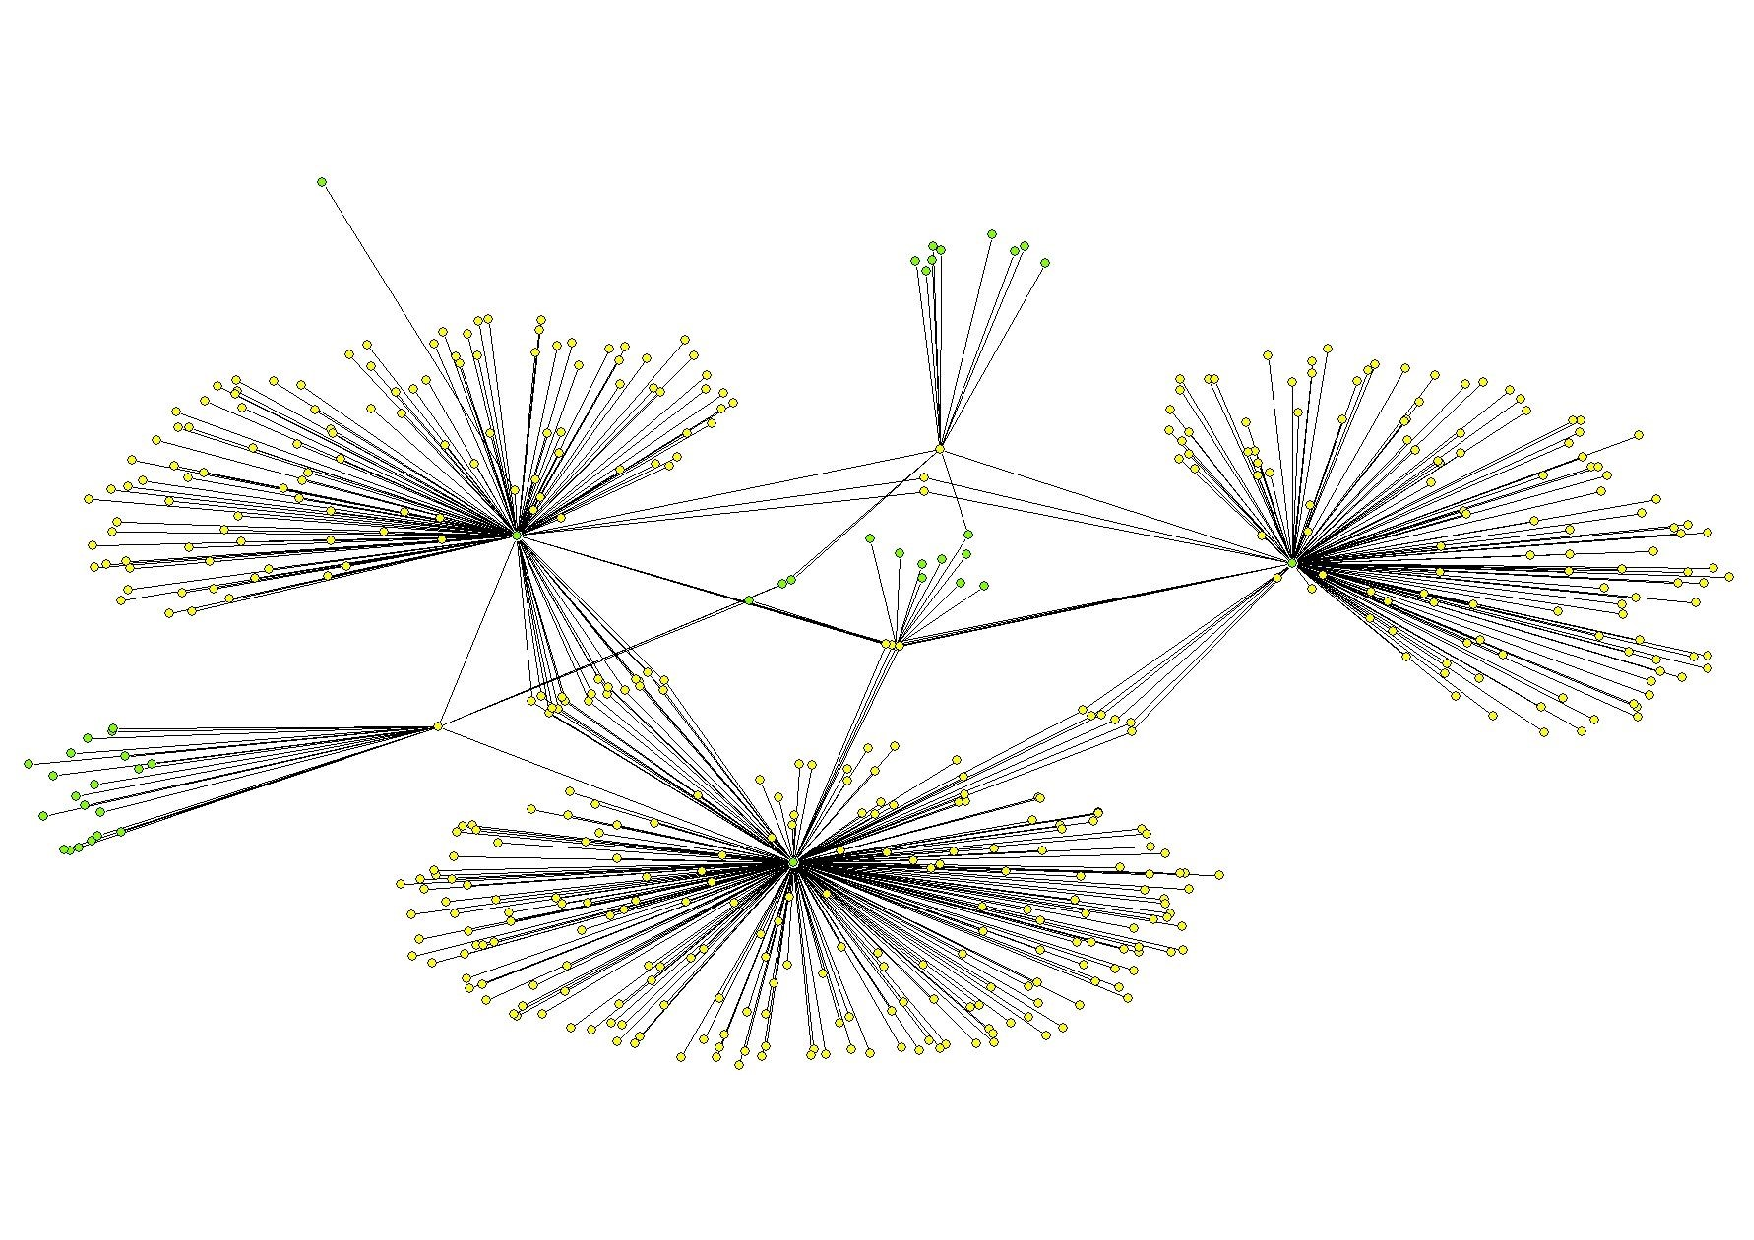
\includegraphics[scale=0.55]{rede_artistas_orquestras_PROVISORIO.pdf}

	%	\fonte{Elaboração do autor a partir de dados disponíveis online}

	%\end{figure}







	\postextual

	\citeoption{abnt-full-initials=yes}

	\bibliography{BIBDOUTORADO, abnt-options}
















	\chapter*[Anexo 1]{Anexo 1 - Investigação Bibliográfica}
        \addcontentsline{toc}{chapter}{Anexo 1 - Investigação Bibliográfica}        

	Com o objetivo de identificar o ``estado da arte"  no campo de pesquisas que envolvem o mercado da música e a economia da música, pesquisamos os \textit{abstracts} de trabalhos publicados na área entre 1983 e 2014 ($n=44$). Para isso, usamos as \textit{keywords} listadas na Figura \ref{chaves-busca} nos indexadores \textit{Sociological Abstracts} e \textit{Econlit}. A grande maioria dos trabalhos encontrados são artigos (86.36\%), quatro são teses de doutorado e dois são livros que foram publicados também a partir de trabalhos de doutorado. Os tipos de estudo mais encontrados na área foram estudos de caso (\textit{Case Studies}), estudos históricos e trabalhos de cunho quantitativo (cf. Tabela \ref{tipo-de-estudo}). Aqui é importante salientar que a codificação dos tipos de estudo foi feita a partir dos resumos consultados tendo como critério a sua citação expressa.

	\begin{figure}[!h]
		\centering
		\caption{Chaves de busca usadas}
		\label{chaves-busca}
		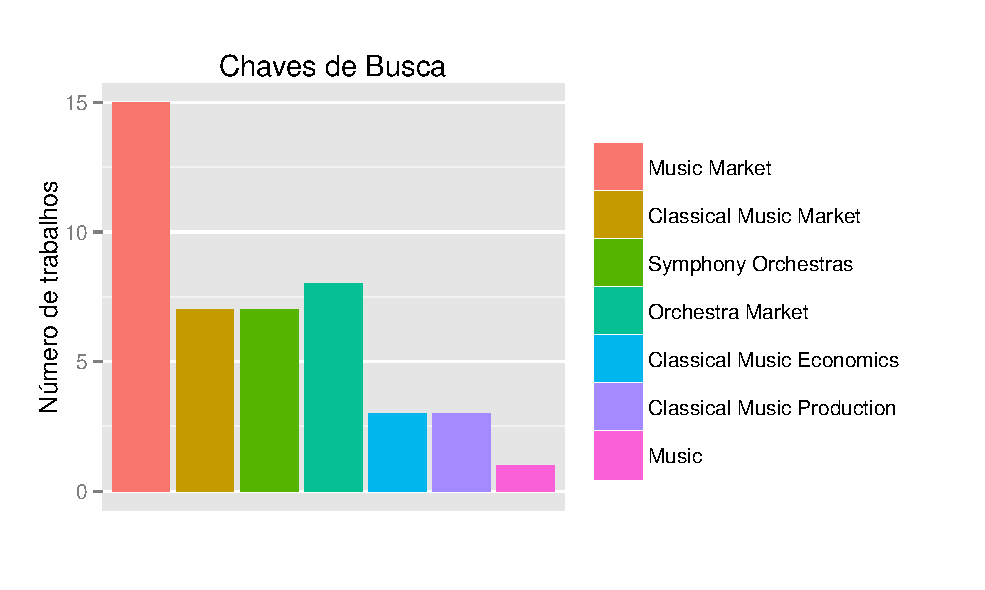
\includegraphics[scale=0.8]{chave.eps}
		\legend{Fonte: Dados trabalhados pelo autor}
	\end{figure}



	Dois estudos experimentais chamaram nossa atenção pela originalidade do desenho metodológico, a saber, \citeonline{salganik2008leading} pela aplicação do método experimental no estudo de um mercado cultural artificial e \citeonline{kasaras2012musical} que também utilizam do método experimental aliado à análise de redes sociais para investigar a influência no gosto musical na Web.  Eles são ainda bem recentes e não estão inseridos, como as outras metodologias, numa tradição de pesquisa em sociologia.

	Os métodos (cf. Tabela \ref{metodos-usados}) mais citados nos resumos foram a \textit{Social Network Analysis}, o \textit{Web-based Experiment} e pesquisas utilizando grandes bancos de dados (\textit{Big Data}) e entrevistas. Após cruzar as frequências dos métodos utilizados com o ano de publicação, investigamos se, de fato há associação entre essas variáveis na amostra calculando o $V$ de Cramér, uma medida para associação de variáveis categóricas. O $V$ de Cramér é definido por $$ V = \sqrt{\frac{\chi^2}{n\cdot(k-1)}} $$ onde $k$ é o menor valor entre o número de linhas e o número de colunas da tabela gerada \cite{barbetta2012estatistica}.

	O valor calculado para estas variáveis foi $V=0.9280$ indicando uma associação muito forte. As variáveis ``Métodos" e "Tipo de estudo" apresentaram associação perfeita. Podemos perceber que os métodos utilizados tem uma mudança mais significativa no tempo do que as metodologias propriamente. É notável a grande variedade de métodos utilizados nessa área de pesquisa. Esse fato aliado ao pequeno número de artigos publicados no espaço de trinta e um anos denota pouca atenção destinada ao campo do mercado da música de concerto o que, \textit{per se}, já justifica nosso esforço.



	% latex table generated in R 3.1.3 by xtable 1.7-4 package

	% Wed Jul 08 11:53:02 2015



	\begin{table}[ht]
		\ibgetab{
		\centering
		\caption{Tipos de Publicação}
	}
		{\begin{tabular}{lr}
			\hline
			\hline
			Artigo &  38 \\
			PhD Dissertation &   4 \\
			Livro &   2 \\
			\hline
			\end{tabular}
		}
		{\fonte{dados trabalhados pelo autor.}}
	\end{table}





	% latex table generated in R 3.1.3 by xtable 1.7-4 package

	% Wed Jul 08 11:56:08 2015

			\begin{table}[ht]
				\ibgetab{
				\centering
				\caption{Tipo de Estudo}
				\label{tipo-de-estudo}
			}
				{\begin{tabular}{lr}
					\hline
					\hline
					Case Study &   6 \\
					Experimental Study &   2 \\
					Estudo exploratório &   1 \\
					Estudo histórico &   6 \\
					Qualitativo &   1 \\
					Quantitativo &   5 \\
					Sociologia Econômica &   1 \\
					Institutionalist Economic Sociology &   1 \\
					\hline
					\end{tabular}
				}
				{\fonte{dados trabalhados pelo autor.}}
			\end{table}





	% latex table generated in R 3.1.3 by xtable 1.7-4 package

	% Wed Jul 08 11:57:57 2015

					\begin{table}[ht]
						\ibgetab{
						\centering
						\caption{Métodos usados}
						\label{metodos-usados}
					}
						{\begin{tabular}{lr}
							\hline
							\hline
							Multivariate Regression Analysis &   1 \\
							Big Data &   1 \\
							Big Data + Word Count &   1 \\
							Comparative Analysis &   1 \\
							Comparative Historical Analysis &   1 \\
							Discourse Analysis &   1 \\
							Método Econômico &   1 \\
							Field Theory / Organizational Theory &   1 \\
							Pesquisa Documental &   1 \\
							Racionalização &   1 \\
							Social Network Analysis &   3 \\
							Survey &   1 \\
							Web-based Experiment &   2 \\
							Interviews + Documentation Analysis + Statistics  &  1 \\
							Interviews + Music Journals + Promotional Literature &   1 \\
							\hline
						\end{tabular}
					}
					{\fonte{dados trabalhados pelo autor.}}
					\end{table}







	%				\begin{figure}

	%					\caption{Tipos de publicação e métodos utilizados por ano}

	%					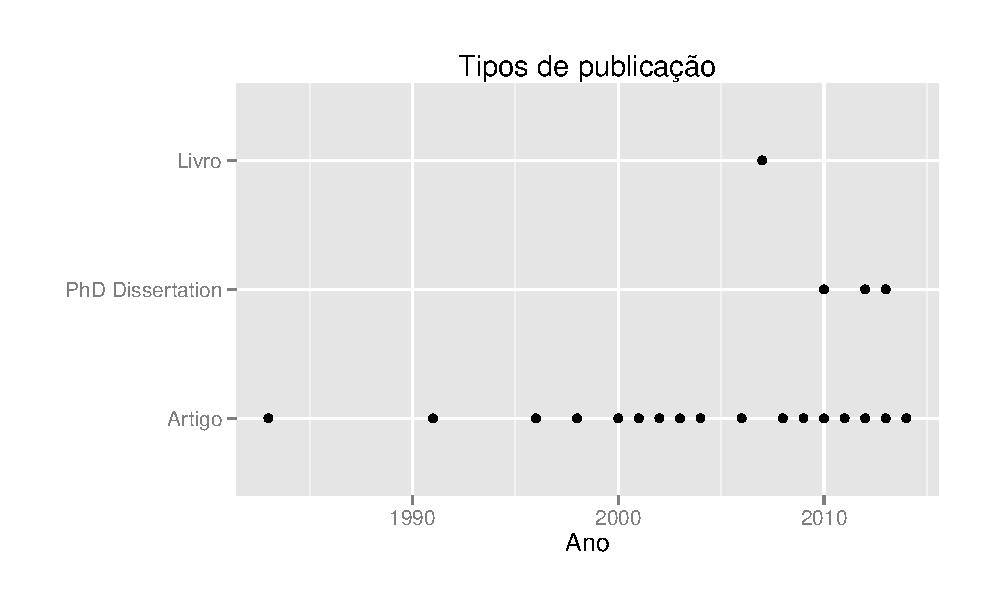
\includegraphics[scale=0.5]{tipopubano.eps}

	%					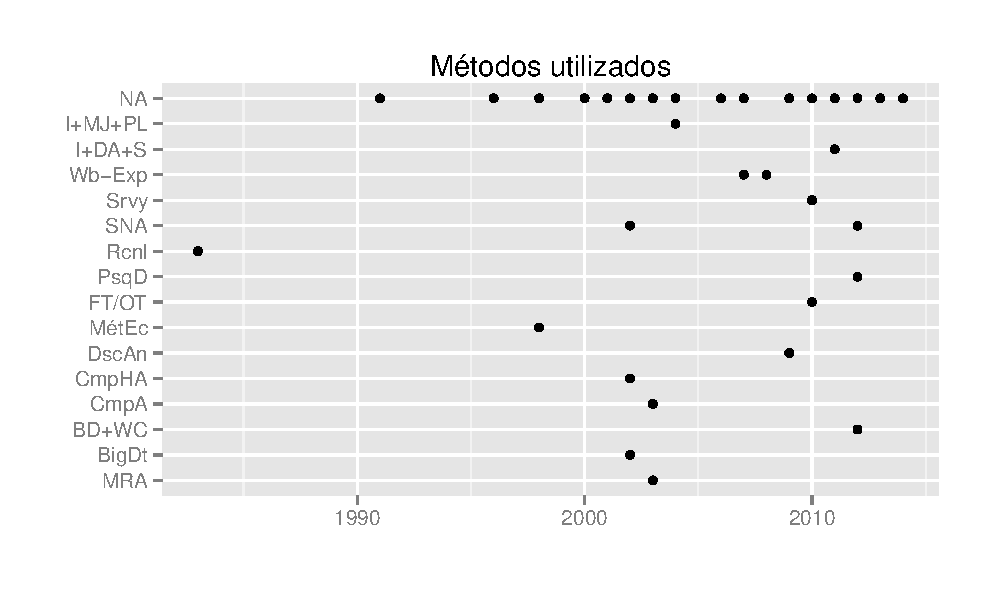
\includegraphics[scale=0.5]{metodoanoab.eps}

	%					\legend{Fonte: Dados trabalhados pelo autor}

	%				\end{figure}



	%\begin{figure}

	%	\caption{Métodos utilizados por ano}

	%	\includegraphics[scale=1]{metodoanoab.eps}

	%	\legend{Fonte: Dados trabalhados pelo autor}

	%\end{figure}



	%				\begin{figure}

	%					\centering

	%					\caption{Densidade de publicações por ano}

	%					\includegraphics[scale=0.5]{tipoestudoano.eps}

	%					\includegraphics[scale=0.7]{anodensidade.eps}

	%					\legend{Fonte: Dados trabalhados pelo autor}

	%				\end{figure}



	O gráfico de densidade\footnote{Um gráfico de densidade mostra a propabilidade de as observações cairem numa janela de variação ao longo da variável de interesse. Em contraposição ao histograma que mostra uma medida discreta, o gráfico de densidade mostra um contínuo de distribuição dessas probabilidades \cite{lander2014r}.} na figura \ref{grafico-densidade} gerado a partir dos anos de publicação (Figura 3) mostra que, nos trinta e um anos analisados, o campo tem crescido. Este crescimento, entretanto, se deu mais efetivamente nos últimos quinze anos. A densidade das publicações até 1995 é bastante baixa.



	\begin{figure}
		\centering
		\caption{Densidade de publicações por ano}
		\label{grafico-densidade}
		\includegraphics[scale=.6]{anodensidade.eps}
		\legend{Fonte: Dados trabalhados pelo autor}
	\end{figure}




		Os temas de investigação aparecem nos trabalhos de uma maneira bastante difusa. Encontramos algumas publicações abordando aspectos culturais que influenciam o mercado da música, o mercado de trabalho dos músicos, as relações de gênero e a divisão do trabalho, financiamento e ``patronagem", o consumo da música e as variáveis que o explicam, gosto musical, padrões estéticos, identidade cultural e música nacional/folclórica, história social dos músicos, o ``cânon" do repertório musical, liderança do maestro e participação e satisfação dos músicos, música antiga\footnote{No campo da música, convencionou-se chamar de música antiga aquela escrita até o séc. XVII.}, revolução digital e indústria fonográfica.

		Percebemos algumas leves polarizações entre os autores expressamente citados nos resumos. Um deles é Bourdieu que, conhecidamente, deixou um vasto trabalho na área de sociologia da arte e do consumo de arte. O nome de Viviana Zelizer aparece relacionado ao de Bourdieu em um resumo consultado. Stigler e Becker são citados num trabalho que argumenta contra a perspectiva econômica neoclássica. Matthew Salganik também aparece nessa bibliografia como autor de dois trabalhos e é citado por mais um indicando novamente atenção ao método experimental na área. No campo, alguns trabalhos tendem a seguir uma perspectiva teórica que privilegia a influência dos aspectos culturais na economia (sociologia econômica). No entanto, não há uma corrente teórica definida perceptível, o que indica que a área não é madura e nem tem uma tradição de pesquisas consolidada.

		Apresentamos a seguir um quadro contendo autor, ano, periódico de publicação e principais assuntos de todos os trabalhos aqui investigados. Pelo fato de que todas referências encontradas são apenas tangenciais ao nosso objeto de pesquisa, nenhuma delas foi revisada em profundidade. O mérito desta investigação bibliográfica preliminar consiste justamente do reconhecimento de que nosso objeto de pesquisa permanece até hoje praticamente inexplorado em suas particularidades.






	\begin{SingleSpace}

	\begin{footnotesize}

	\begin{center}



	\begin{longtable}{p{4cm}lp{4cm}p{4cm}}







		\hline

		\textbf{Autores} &\textbf{Ano} & \textbf{Journal} & \textbf{Assunto}\\

		\hline

		\hline

		\endfirsthead

		\hline

		\endhead

		\hline

		\endfoot

		\hline

		\hline

		\endlastfoot



		Roy, Tirthankar & 1998 & Contributions to Indian Sociology & Indian classical music\\

		Waterman, Stanley & 2010 & Contemporary Jewry & Israel culture/music\\

		Coaldrake, Kimi	& 2012 & Japanese Studies & Japanese popular music\\

		Menger, Pierre-Michel & 1991 & Cahiers de recherche sociologique & Factors affecting market structure and music evaluation\\

		Menger, Pierre-Michel & 1983 & Sociologie du Travail & Division of musical labor\\

		Buchholz, Larissa & 2013 & NA & Global rules of art\\

		Etzioni, Amitai & 1998 & Journal of Socio-Economics & Taste for classical music\\

		Roebuck, James C & 2000 & American Sociological Association & Gendered-habitus, and the sexual division of labor\\

		Francois, Pierre & 2004 & Sociologie du Travail & Ilness of cost / concert market / musicians labor market\\

		Gligorijevic, Jelena & 2014 & International Journal of Cultural Policy & Music festival / Serbia\\

		Hofman, Ana & 2014 & Dve domovini / Two Homelands & Identification and affiliation / trumpet orchestra music / Balkan music\\

		Segnini, Liliana Rolfsen Petrilli & 2011 & Estudos de Sociologia & Music job market\\

		Epstein, Louis K & 2013 & NA & Music patronage\\

		Kaleta, Andrzej & 2004 & Polish Sociological Review & Cultural Activity of Rural Inhabitants\\

		Zolberg, Vera & 1996 & International Sociology & Music patronage\\

		Mauskapf, Michael G & 2012 & NA & Music patronage / economic and cultural sustainability\\

		Borowiecki, Karol J; O'Hagan, John W & 2012 & Historical Social Research/Historische Sozialforschung & Historical Patterns / The case of classical composers\\

		Fisher, Timothy C G; Preece, Stephen B & 2003 & Poetics & Culture of comsumption\\

		Dowd, Timothy J; Liddle, Kathleen; Lupo, Kim; Borden, Anne. & 2002 & Poetics & Musical Canon\\

		Kremp, Pierre-Antoine & 2010 & Social Forces & Musical Canon\\

		Broughton, Andrea & 2001 & European Journal of Industrial Relations & Collective Bargaining in the Arts and Culture Sector\\

		Hughes, Patricia; Luksetich, William; Rooney, Patrick & 2014 & Nonprofit Management \& Leadership & Music patronage\\

		Glynn, Mary Ann & 2002 & Poetics & Organizational Crisis / Institutional Shifts / Musical Canon\\

		Wood, Roy D & 2010 & NA & Conductor leadership style, musician employment status, organizational participation to orchestra musician job satisfaction\\

		Bijsterveld, Karin; Schulp, Marten & 2004 & Social Studies of Science & Innovation in classical music instruments\\

		Luthje, Corinna & 2010 & Medien \& Kommunikationswissenschaft & Classical Music in German Commercial Radio Programming\\

		McCormick, Lisa & 2009 & Cultural Sociology & International Music Competition\\

		Lee, Steve Sungchu & 2007 & NA & Musical stratification / aesthetics\\

		Francois, Pierre & 2006 & Revue francaise de Sociologie & Early Music Market\\

		Santoro, Marco & 2013 & European Societies & Institutions / music market\\

		Abreu, Paula & 2009 & Revista Critica de Ciencias Sociais & Portuguese phonographic industry\\

		Watson, Allan & 2012 & Global Networks & Urban networks of music production / Itunes\\

		Nicolau, Michel & 2010 & International Sociological Association & National Identity / Brazilian music\\

		Janowska, Anna Anetta & 2011 & Societes & Digital Revolution / Reconrding Industry\\

		Abreu, Paula & 2004 & Revista Critica de Ciencias Sociais & Territorial dynamics of cultural markets / Portuguese music\\

		Shin, Eui Hang; Oh, Joong-Hwan & 2002 & East Asia: An International Quarterly & Relationships between two different sets of actors - songwriters \& singers / Korean popular music industry\\

		Salganik, Matthew J; Watts, Duncan J & 2008 & Social Psychology Quarterly & Self-fulfilling Prophecies in an Artificial Cultural Market\\

		Dowd, Timothy J & 2003 & Comparative Social Research & Structural Power and the Construction of Markets / R\&B\\

		DeNora, Tia & 2013 & European Societies & Markets and socio-cultural practices\\

		Menger, Pierre-Michel & 2002 & Annales & Genius / Beethoven\\

		Pethig, Rudiger; Cheng, Sao-Wen & 2002 & Schmollers Jahrbuch & Cultural Capital / Consumption of Cultural Services\\

		Salganik, Matthew J & 2007 & NA & Success and failure in cultural markets\\

		Kasaras, Kostas; Klimis, George Michael; Michailidou, Martha & 2012 & Contemporary Social Science: Journal of the Academy of Social Sciences & Musical tastes / experimental study\\

		Ginsburgh, Victor & 2003 & Journal of Economic Perspectives & Expertise in the arts influence success\\



	\end{longtable}

\end{center}

\end{footnotesize}

\end{SingleSpace}






	\chapter*[Anexo 2]{Anexo 2 - Questionário online}

	\addcontentsline{toc}{chapter}{Anexo 2 - Questionário online}



	[\textbf{Primeira página - Concordância}]
	
	QUESTIONÁRIO SOCIOMÉTRICO DIRECIONADO A MÚSICOS E PROFESSORES
	
	Olá. A pesquisa de tese em andamento intitulada ``A Construção Social da Qualidade num Mercado de Música de Concerto'' de autoria de Neylson Crepalde visa investigar a construção de um padrão de qualidade amplamente aceito por orquestras, músicos e público com o qual todos assumem compromisso e sobre o qual todos agem na construção do mercado da música de concerto. O estudo está sendo realizado de uma perspectiva relacional. Desse modo, uma parte das perguntas a serem feitas aos entrevistados são o que a literatura chama de “geradores de nomes”, ou seja, perguntas que demonstram algum tipo de relação entre dois indivíduos ou organizações.
	
	Um dos principais objetivos do estudo é reconstruir a estrutura de relações entre músicos e entre organizações para, a partir dela, entender como emerge o conceito de qualidade.
	
	A tese está sendo orientada pelo professor Silvio Salej Higgins (UFMG/Brasil) e tem coorientação do prof. Emmanuel Lazega (CSO – SciencesPo/França).
	
	Muito embora esta pesquisa de tese não tenha passado por nenhum comitê de ética em pesquisa, todos os procedimentos éticos recomendados estão sendo adotados. Nenhum nome, seja de organização ou indivíduo será divulgado (a menos que haja expresso desejo da organização ou indivíduo) e a participação é voluntária. Os participantes possuem o direito de retirar sua participação a qualquer momento da pesquisa. É importante, entretanto, salientar o quão importante é a participação de cada convidado para o sucesso da pesquisa de tese.
	
	Para quaisquer dúvidas ou esclarecimentos, os contatos dos responsáveis pela pesquisa estão disponibilizados abaixo:
	
	Neylson Crepalde – Doutorando
	Telefone: +55 31 98554 0770
	E-mail: neylsoncrepalde@gmail.com
	
	Silvio Salej Higgins – Orientador
	E-mail: sisahi@yahoo.com.br
	
	\vspace{1cm}
	
	[\textbf{Segunda Página - Informações gerais}] % UNDER CONSTRUCTION......
	
	\begin{enumerate}
		\item Qual é o seu nome: 
		
		\item Sexo?
		\begin{itemize}
			\item Masculino
			\item Feminino
			\item Outro
		\end{itemize}
		
		\item Qual é a sua escolaridade?
		\begin{itemize}
			\item Ensino médio - incompleto
			\item Ensino médio - completo
			\item Superior - incompleto
			\item Superior - completo
			\item Mestrado - incompleto
			\item Mestrado - completo
			\item Doutorado - incompleto
			\item Doutorado - completo
		\end{itemize}
		
		\item Quanto à cor da pele, o(a) senhor(a) se considera...?
		\begin{itemize}
			\item Branco
			\item Preto
			\item Pardo
			\item Amarelo
			\item Indígena
			\item Outro
		\end{itemize}
		
		\item Qual é a sua idade?
		

		\item Qual é o seus estado civil?
		\begin{itemize}
			\item Casado
			\item Solteiro
			\item Divorciado
			\item Viúvo
			\item Outro
		\end{itemize}
		
		
		\item O(a) senhor(a) tem filhos? Quantos?
		
		
		[\textbf{Terceira página - Atividades musicais}]  
		
		
		\item Qual é a sua principal atividade como músico?
		\begin{itemize}
			\item Intrumentista
			\item Cantor
			\item Maestro
			\item Professor
			\item Outro
		\end{itemize}
		
		

		
		\item O(a) senhor(a) toca em alguma orquestra? Qual ou quais?
		
		\item O(a) senhor(a) ensina em alguma escola de música, faculdade/universidade? Qual?
		\item Se sim, quantos alunos possui hoje?
		\item Qual foi a sua renda total no último mês considerando todas as orquestras nas quais o(a) senhor(a) tocou?
		\item Qual foi a sua renda total no último mês considerando seu trabalho com as orquestras e todas as outras atividades que o(a) senhor(a) exerce?
		
		\item Com que frequência o(a) senhor(a) assiste a concertos?
		\begin{itemize}
			\item Uma ou duas vezes por ano
			\item Uma ou duas vezes a cada três meses
			\item Uma ou duas vezes por mês
			\item Uma vez por semana
			\item Mais de uma vez por semana
		\end{itemize}
		
		
		
		[\textbf{Quarta página - Bloco relacional}]
		
		
		\item Se o(a) senhor(a) precisasse de aconselhamento sobre a interpretação de alguma peça, independente do período ou do estilo da obra, a quem o(a) senhor(a) pediria conselho? Mencione quantas pessoas o(a) senhor(a) quiser.
		
		\item O(a) senhor(a) costuma se encontrar com outros músicos em ocasiões sociais fora do horário de trabalho? Com quem o(a) senhor(a) se encontra? Mencione quantas pessoas o(a) senhor(a) quiser.
		
		\item Se o(a) senhor(a) fosse indicar um músico para uma excelente posição em uma orquestra, a quem o(a) senhor(a) indicaria? Mencione quantas pessoas o(a) senhor(a) quiser independente do instrumento.
		
		\item Se o(a) senhor(a) fosse responsável por organizar um recital ou um concerto no qual o(a) senhor(a) fosse tocar, independente da instrumentação das obras que o senhor poderia escolher, a quem o(a) senhor(a) convidaria para tocar com o(a) senhor(a)? Mencione quantas pessoas o(a) senhor(a) quiser.
		
		\item Para o(a) senhor(a), quais são as orquestras em Belo Horizonte que possuem a melhor qualidade? Por favor, cite da que possui a melhor qualidade para a que possui a pior dentre elas.
		
		\item Porque a orquestra que o(a) senhor(a) disse ser a melhor é a melhor? Cite quantas razões o(a) senhor(a) quiser.
		
		\item Caso o(a) senhor(a) seja também professor(a), como o(a) senhor(a) faz seus alunos entenderem o que é necessário para uma boa performance?
		
		
		
		
		[\textbf{Quinta página - Bloco Contextual}]
		
		
		\item Em qual país o(a) senhor(a) nasceu?
		\item Em qual cidade o(a) senhor(a) nasceu?
		\item Por quantos ANOS o(a) senhor(a) estuda música?
		\item Por quantos ANOS o(a) senhor(a) tem trabalhado como músico/musicista profissional?
		\item Em qual instituição o(a) senhor(a) recebeu a maior parte de sua educação musical?
		\item E em segundo lugar?
		\item Com qual professor o(a) senhor(a) estudou pelo período mais longo?
		\item E em segundo lugar?
		
	\end{enumerate}
	
	Muito obrigado pela sua participação. Sua colaboração é imprescindível para o sucesso dessa pesquisa. Novamente, muito obrigado!
	
	

	
	
	
	\chapter*[Anexo 3]{Anexo 3 -- Questionário sociométrico - organizações}

        \addcontentsline{toc}{chapter}{Anexo 3 - Questionário sociométrico - organizações}
	
	%Good day. I want to thank you very much for your participation and assure that it is extremely important for the success of this PhD research.
	
	Bom dia. Quero agradecer muitíssimo pela sua participação e assegurar o quanto ela é importante para o sucesso desta pesquisa de Doutorado.
	
	\vspace{1cm}
	\begin{enumerate}
		%\item Let's start with your professional partnerships. Could you name all the professionals that you relate with regularly? By professionals I mean every company with whom you have relations, economic or other, for example, advisement, collaboration, resources exchange, etc.
		
		\item Vamos começar com suas parcerias profissionais. O senhor poderia nomear todos os empresas com as quais a organização se relaciona regularmente? Me refiro aqui a qualquer companhia com a qual a orquestra tenha relações, econômicas ou de outra natureza, como por exemplo, aconselhamento, colaboração, troca de recursos, etc.
		
		%\item What is the main activity of each of these professionals?
		
		\item Vamos retomar cada uma dessas empresas. Qual é a principal atividade de cada uma delas?
		
		%\item I would like to retake each of this professionals that you mentioned. What is the relation that you would say you have with each one of them?
		
		\item Vamos retomar mais uma vez a lista de empresas que o senhor mencionou. Qual é a relação que o senhor diria que a orquestra possui com cada um?
		\begin{itemize}
			\item Uma relação de fornecedor e cliente, apenas.
			\item Uma parceria
			\item Uma colaboração
			\item Uma relação de aconselhamento
			\item Outra
		\end{itemize}
		
		%\item What is the organization's structure? Is there an organizational chart that I could consult?
		\item Qual é a estrutura da organização? Existe um organograma que eu possa consultar?
		
		%\item What is the organization's budget?     
		
		\item Qual é o orçamento total da organização?
		
		%\item You did mention the State as one of your partners (What about the State?) How many contracts do you have with the State? What is it's share in your budget?
		
		\item O senhor mencionou o Estado como um de seus parceiros (E o Estado?) Quantos contratos a orquestra possui com o Estado? Qual é a sua parcela de contribuição no orçamento?
		
		%\item What would you say is your organization's style within the market?
		

		%\item In what spaces does the orchestra usually play? How many seats available?
		
		\item Em quais espaços a orquestra normalmente toca? Quantos assentos tem disponíveis em cada um?
		
		%\item What is the ticket price for each of the concert series? Is there variation on ticket price according to the place in the concert room? How many tickets are made available with each price?
		\item Qual é o preço do ingresso para cada série de concertos? Há uma variação no preço de acordo com o lugar na sala? Quantos ingressos são disponibilizados por cada faixa de preço?
		
		%\item How much does the organization spend with musicians paycheck?
		\item Quanto a orquestra gasta com a folha de pagamento dos músicos?
		
		%\item Besides musicians and guests paycheck, what would you say are other artistic expenses of a performance?
		\item Além da folha de pagamento dos músicos e convidados, o senhor diria que há outras despesas artísticas relacionadas às performances?
		
		%\item Does the orchestra have some incentive for the musicians to feel motivated, pleased and satisfied with their jobs? Could you list them, please?
		\item A orquestra oferece incentivos aos músicos para que eles se sintam motivados, felizes e satisfeitos com seu emprego? O senhor poderia listá-los, por favor?
		
	\end{enumerate}
	
	Muito obrigado pela participação!




	\chapter*[Anexo 4]{Anexo 4 - Medidas de centralidade e constraint para as redes observadas}

        \addcontentsline{toc}{chapter}{Anexo 4 - Medidas de centralidade e constraint para as redes observadas}

		\begin{SingleSpace}
		\begin{footnotesize}
			\begin{center}
				\begin{longtable}{c c c c c}
					\caption{Medidas de centralidade e constraint da rede de aconselhamento}\\
					\label{centralidades:conselho}\\
					\hline
					\textbf{ID}  & \textbf{Indegree} & \textbf{Betweeness} & \textbf{Closeness} & \textbf{Constraint} \\
					\hline
					\endfirsthead
					\hline
					\endhead
					\hline
					\endfoot
					\hline
					\multicolumn{5}{l}{Fonte: Elaboração do autor}\\
					\endlastfoot
					V1 & 0 & 0 & 0.015 & 0.2 \\ 
					V2 & 1 & 0 & 0.014 & 1 \\ 
					V3 & 0 & 0 & 0.015 & 0.333 \\ 
					V4 & 1 & 0 & 0.014 & 1 \\ 
					V5 & 0 & 0 & 0.015 & 0.333 \\ 
					V6 & 1 & 0 & 0.014 & 1 \\ 
					V7 & 1 & 10.5 & 0.017 & 0.083 \\ 
					V8 & 2 & 0 & 0.014 & 0.5 \\ 
					V9 & 0 & 0 & 0.016 & 0.111 \\ 
					V10 & 1 & 0 & 0.014 & 1 \\ 
					V11 & 0 & 0 & 0.017 & 0.5 \\ 
					V12 & 0 & 0 & 0.016 & 0.125 \\ 
					V13 & 2 & 0 & 0.014 & 0.5 \\ 
					V14 & 0 & 0 & 0.014 & 1 \\ 
					V15 & 1 & 0 & 0.014 & 1 \\ 
					V16 & 0 & 0 & 0.014 & 1 \\ 
					V17 & 1 & 0 & 0.014 & 1 \\ 
					V18 & 1 & 0 & 0.014 & 0 \\ 
					V19 & 0 & 0 & 0.014 & 0.5 \\ 
					V20 & 1 & 0 & 0.014 & 1 \\ 
					V21 & 0 & 0 & 0.014 & 1 \\ 
					V22 & 1 & 0 & 0.014 & 1 \\ 
					V23 & 0 & 0 & 0.014 & 1 \\ 
					V24 & 1 & 0 & 0.014 & 1 \\ 
					V25 & 0 & 0 & 0.015 & 0.333 \\ 
					V26 & 1 & 0 & 0.014 & 1 \\ 
					V27 & 0 & 0 & 0.015 & 0.333 \\ 
					V28 & 1 & 0 & 0.014 & 1 \\ 
					V29 & 0 & 0 & 0.014 & 1 \\ 
					V30 & 1 & 0 & 0.014 & 1 \\ 
					V31 & 1 & 1.5 & 0.014 & 0.333 \\ 
					V32 & 1 & 0 & 0.014 & 1 \\ 
					V33 & 0 & 0 & 0.015 & 0.333 \\ 
					V34 & 1 & 0 & 0.014 & 1 \\ 
					V35 & 0 & 0 & 0.015 & 0.25 \\ 
					V36 & 2 & 0 & 0.014 & 0.5 \\ 
					V37 & 1 & 0 & 0.014 & 1 \\ 
					V38 & 3 & 0 & 0.014 & 0.333 \\ 
					V39 & 1 & 0 & 0.014 & 1 \\ 
					V40 & 1 & 0 & 0.014 & 1 \\ 
					V41 & 1 & 0 & 0.014 & 1 \\ 
					V42 & 2 & 0 & 0.014 & 0.5 \\ 
					V43 & 1 & 0 & 0.014 & 1 \\ 
					V44 & 2 & 0 & 0.014 & 0.5 \\ 
					V45 & 1 & 0 & 0.014 & 1 \\ 
					V46 & 1 & 0 & 0.014 & 1 \\ 
					V47 & 1 & 0 & 0.014 & 1 \\ 
					V48 & 1 & 0 & 0.014 & 1 \\ 
					V49 & 1 & 0 & 0.014 & 1 \\ 
					V50 & 2 & 0 & 0.014 & 0.5 \\ 
					V51 & 1 & 0 & 0.014 & 1 \\ 
					V52 & 1 & 0 & 0.014 & 1 \\ 
					V53 & 1 & 0 & 0.014 & 1 \\ 
					V54 & 1 & 0 & 0.014 & 1 \\ 
					V55 & 2 & 0 & 0.014 & 0.5 \\ 
					V56 & 1 & 0 & 0.014 & 1 \\ 
					V57 & 1 & 0 & 0.014 & 1 \\ 
					V58 & 1 & 0 & 0.014 & 1 \\ 
					V59 & 1 & 0 & 0.014 & 1 \\ 
					V60 & 1 & 0 & 0.014 & 1 \\ 
					V61 & 1 & 0 & 0.014 & 1 \\ 
					V62 & 1 & 0 & 0.014 & 1 \\ 
					V63 & 1 & 0 & 0.014 & 1 \\ 
					V64 & 1 & 0 & 0.014 & 1 \\ 
					V65 & 1 & 0 & 0.014 & 1 \\ 
					V66 & 1 & 0 & 0.014 & 1 \\ 
					V67 & 1 & 0 & 0.014 & 1 \\ 
					V68 & 1 & 0 & 0.014 & 1 \\ 
					V69 & 1 & 0 & 0.014 & 1 \\ 
					V70 & 1 & 0 & 0.014 & 1 \\ 
					V71 & 1 & 0 & 0.014 & 1 \\ 
					
				\end{longtable}
			\end{center}
		\end{footnotesize}
	\end{SingleSpace}
	


		\begin{SingleSpace}
		\begin{footnotesize}
			\begin{center}
				\begin{longtable}{c c c c c}
					\caption{Medidas de centralidade e constraint da rede de amizade}\\
					\label{centralidades:amizade}\\
					\hline
					\textbf{ID}  & \textbf{Indegree} & \textbf{Betweeness} & \textbf{Closeness} & \textbf{Constraint} \\
					\hline
					\endfirsthead
					\hline
					\endhead
					\hline
					\endfoot
					\hline
					\multicolumn{5}{l}{Fonte: Elaboração do autor}\\
					\endlastfoot
					V1 & 0 & 0 & 0.016 & 0.25 \\ 
					V2 & 3 & 0 & 0.015 & 0.333 \\ 
					V3 & 0 & 0 & 0.017 & 0.143 \\ 
					V4 & 1 & 0 & 0.015 & 1 \\ 
					V5 & 0 & 0 & 0.018 & 0.313 \\ 
					V6 & 2 & 0 & 0.015 & 0.5 \\ 
					V7 & 2 & 9 & 0.018 & 0.261 \\ 
					V8 & 3 & 14 & 0.018 & 0.239 \\ 
					V9 & 0 & 0 & 0.016 & 0.2 \\ 
					V10 & 1 & 0 & 0.015 & 1 \\ 
					V11 & 0 & 0 & 0.019 & 0.242 \\ 
					V12 & 0 & 0 & 0.018 & 0.1 \\ 
					V13 & 1 & 0 & 0.015 & 1 \\ 
					V14 & 0 & 0 & 0.015 & NaN \\ 
					V15 & 0 & 0 & 0.015 & NaN \\ 
					V16 & 0 & 0 & 0.015 & 1 \\ 
					V17 & 1 & 0 & 0.015 & 1 \\ 
					V18 & 0 & 0 & 0.016 & 0.333 \\ 
					V19 & 1 & 0 & 0.015 & 1 \\ 
					V20 & 0 & 0 & 0.016 & 0.5 \\ 
					V21 & 1 & 0 & 0.015 & 1 \\ 
					V22 & 0 & 0 & 0.015 & NaN \\ 
					V23 & 0 & 0 & 0.015 & NaN \\ 
					V24 & 0 & 0 & 0.015 & NaN \\ 
					V25 & 0 & 0 & 0.016 & 0.25 \\ 
					V26 & 1 & 0 & 0.015 & 1 \\ 
					V27 & 0 & 0 & 0.015 & NaN \\ 
					V28 & 0 & 0 & 0.016 & 0.2 \\ 
					V29 & 1 & 0 & 0.015 & 1 \\ 
					V30 & 1 & 0 & 0.015 & 1 \\ 
					V31 & 1 & 0 & 0.015 & 1 \\ 
					V32 & 2 & 0 & 0.015 & 0.5 \\ 
					V33 & 1 & 0 & 0.015 & 1 \\ 
					V34 & 1 & 0 & 0.015 & 1 \\ 
					V35 & 1 & 0 & 0.015 & 1 \\ 
					V36 & 1 & 0 & 0.015 & 1 \\ 
					V37 & 1 & 0 & 0.015 & 1 \\ 
					V38 & 2 & 0 & 0.015 & 0.764 \\ 
					V39 & 2 & 0 & 0.015 & 0.5 \\ 
					V40 & 2 & 0 & 0.015 & 0.5 \\ 
					V41 & 1 & 0 & 0.015 & 1 \\ 
					V42 & 3 & 0 & 0.015 & 0.553 \\ 
					V43 & 2 & 0 & 0.015 & 0.5 \\ 
					V44 & 1 & 0 & 0.015 & 1 \\ 
					V45 & 1 & 0 & 0.015 & 1 \\ 
					V46 & 1 & 0 & 0.015 & 1 \\ 
					V47 & 1 & 0 & 0.015 & 1 \\ 
					V48 & 1 & 0 & 0.015 & 1 \\ 
					V49 & 1 & 0 & 0.015 & 1 \\ 
					V50 & 1 & 0 & 0.015 & 1 \\ 
					V51 & 1 & 0 & 0.015 & 1 \\ 
					V52 & 1 & 0 & 0.015 & 1 \\ 
					V53 & 1 & 0 & 0.015 & 1 \\ 
					V54 & 1 & 0 & 0.015 & 1 \\ 
					V55 & 1 & 0 & 0.015 & 1 \\ 
					V56 & 1 & 0 & 0.015 & 1 \\ 
					V57 & 1 & 0 & 0.015 & 1 \\ 
					V58 & 1 & 0 & 0.015 & 1 \\ 
					V59 & 1 & 0 & 0.015 & 1 \\ 
					V60 & 1 & 0 & 0.015 & 1 \\ 
					V61 & 1 & 0 & 0.015 & 1 \\ 
					V62 & 1 & 0 & 0.015 & 1 \\ 
					V63 & 1 & 0 & 0.015 & 1 \\ 
					V64 & 1 & 0 & 0.015 & 1 \\ 
					V65 & 1 & 0 & 0.015 & 1 \\ 
					V66 & 1 & 0 & 0.015 & 1 \\ 
					
				\end{longtable}
			\end{center}
		\end{footnotesize}
	\end{SingleSpace}
	
	
		\begin{SingleSpace}
		\begin{footnotesize}
			\begin{center}
				\begin{longtable}{c c c c c}
					\caption{Medidas de centralidade e constraint da rede de indicação}\\
					\label{centralidades:indicacao}\\
					\hline
					\textbf{ID}  & \textbf{Indegree} & \textbf{Betweeness} & \textbf{Closeness} & \textbf{Constraint} \\
					\hline
					\endfirsthead
					\hline
					\endhead
					\hline
					\endfoot
					\hline
					\multicolumn{5}{l}{Fonte: Elaboração do autor}\\
					\endlastfoot
					V1 & 0 & 0 & 0.015 & 0.333 \\ 
					V2 & 1 & 0 & 0.014 & 1 \\ 
					V3 & 0 & 0 & 0.017 & 0.261 \\ 
					V4 & 4 & 0 & 0.014 & 0.369 \\ 
					V5 & 0 & 0 & 0.014 & NaN \\ 
					V6 & 4 & 16 & 0.016 & 0.185 \\ 
					V7 & 5 & 0 & 0.014 & 0.271 \\ 
					V8 & 0 & 0 & 0.015 & 0.5 \\ 
					V9 & 4 & 0 & 0.014 & 0.28 \\ 
					V10 & 0 & 0 & 0.017 & 0.188 \\ 
					V11 & 0 & 0 & 0.017 & 0.174 \\ 
					V12 & 3 & 0 & 0.014 & 0.333 \\ 
					V13 & 0 & 0 & 0.018 & 0.083 \\ 
					V14 & 1 & 0 & 0.014 & 1 \\ 
					V15 & 0 & 0 & 0.015 & 0.5 \\ 
					V16 & 1 & 0 & 0.014 & 1 \\ 
					V17 & 0 & 0 & 0.015 & 1 \\ 
					V18 & 1 & 0 & 0.014 & 1 \\ 
					V19 & 0 & 0 & 0.016 & 0.167 \\ 
					V20 & 1 & 0 & 0.014 & 1 \\ 
					V21 & 0 & 0 & 0.015 & 0.5 \\ 
					V22 & 1 & 0 & 0.014 & 1 \\ 
					V23 & 0 & 0 & 0.014 & NaN \\ 
					V24 & 0 & 0 & 0.015 & 0.333 \\ 
					V25 & 1 & 0 & 0.014 & 1 \\ 
					V26 & 0 & 0 & 0.015 & 1 \\ 
					V27 & 2 & 0 & 0.014 & 0.5 \\ 
					V28 & 0 & 0 & 0.015 & 1 \\ 
					V29 & 1 & 0 & 0.014 & 1 \\ 
					V30 & 0 & 0 & 0.017 & 0.179 \\ 
					V31 & 1 & 0 & 0.014 & 1 \\ 
					V32 & 0 & 0 & 0.015 & 0.25 \\ 
					V33 & 1 & 0 & 0.014 & 1 \\ 
					V34 & 0 & 0 & 0.015 & 0.25 \\ 
					V35 & 3 & 0 & 0.014 & 0.333 \\ 
					V36 & 1 & 0 & 0.014 & 1 \\ 
					V37 & 2 & 0 & 0.014 & 0.5 \\ 
					V38 & 2 & 0 & 0.014 & 0.5 \\ 
					V39 & 1 & 0 & 0.014 & 1 \\ 
					V40 & 1 & 0 & 0.014 & 1 \\ 
					V41 & 1 & 0 & 0.014 & 1 \\ 
					V42 & 1 & 0 & 0.014 & 1 \\ 
					V43 & 1 & 0 & 0.014 & 1 \\ 
					V44 & 1 & 0 & 0.014 & 1 \\ 
					V45 & 1 & 0 & 0.014 & 1 \\ 
					V46 & 1 & 0 & 0.014 & 1 \\ 
					V47 & 1 & 0 & 0.014 & 1 \\ 
					V48 & 2 & 0 & 0.014 & 0.5 \\ 
					V49 & 2 & 0 & 0.014 & 0.619 \\ 
					V50 & 1 & 0 & 0.014 & 1 \\ 
					V51 & 1 & 0 & 0.014 & 1 \\ 
					V52 & 1 & 0 & 0.014 & 1 \\ 
					V53 & 1 & 0 & 0.014 & 1 \\ 
					V54 & 1 & 0 & 0.014 & 1 \\ 
					V55 & 1 & 0 & 0.014 & 1 \\ 
					V56 & 1 & 0 & 0.014 & 1 \\ 
					V57 & 1 & 0 & 0.014 & 1 \\ 
					V58 & 1 & 0 & 0.014 & 1 \\ 
					V59 & 1 & 0 & 0.014 & 1 \\ 
					V60 & 1 & 0 & 0.014 & 1 \\ 
					V61 & 1 & 0 & 0.014 & 1 \\ 
					V62 & 1 & 0 & 0.014 & 1 \\ 
					V63 & 1 & 0 & 0.014 & 1 \\ 
					V64 & 1 & 0 & 0.014 & 1 \\ 
					V65 & 1 & 0 & 0.014 & 1 \\ 
					V66 & 1 & 0 & 0.014 & 1 \\ 
					V67 & 1 & 0 & 0.014 & 1 \\ 
					V68 & 1 & 0 & 0.014 & 1 \\ 
					V69 & 1 & 0 & 0.014 & 1 \\ 
					
				\end{longtable}
			\end{center}
		\end{footnotesize}
	\end{SingleSpace}
	
	
		\begin{SingleSpace}
		\begin{footnotesize}
			\begin{center}
				\begin{longtable}{c c c c c}
					\caption{Medidas de centralidade e constraint da rede de convites}\\
					\label{centralidades:convite}\\
					\hline
					\textbf{ID}  & \textbf{Indegree} & \textbf{Betweeness} & \textbf{Closeness} & \textbf{Constraint} \\
					\hline
					\endfirsthead
					\hline
					\endhead
					\hline
					\endfoot
					\hline
					\multicolumn{5}{l}{Fonte: Elaboração do autor}\\
					\endlastfoot
					V1 & 0 & 0 & 0.014 & 0.047 \\ 
					V2 & 1 & 0 & 0.009 & 1 \\ 
					V3 & 0 & 0 & 0.01 & 0.25 \\ 
					V4 & 1 & 0 & 0.009 & 1 \\ 
					V5 & 1 & 18 & 0.01 & 0.167 \\ 
					V6 & 1 & 0 & 0.009 & 1 \\ 
					V7 & 3 & 32 & 0.011 & 0.148 \\ 
					V8 & 2 & 0 & 0.009 & 0.602 \\ 
					V9 & 0 & 0 & 0.01 & 0.25 \\ 
					V10 & 4 & 0 & 0.009 & 0.25 \\ 
					V11 & 0 & 0 & 0.012 & 0.141 \\ 
					V12 & 0 & 0 & 0.011 & 0.083 \\ 
					V13 & 3 & 0 & 0.009 & 0.333 \\ 
					V14 & 0 & 0 & 0.012 & 0.067 \\ 
					V15 & 2 & 0 & 0.009 & 0.5 \\ 
					V16 & 1 & 4 & 0.01 & 0.363 \\ 
					V17 & 1 & 0 & 0.009 & 1 \\ 
					V18 & 0 & 0 & 0.01 & 1 \\ 
					V19 & 2 & 0 & 0.009 & 0.5 \\ 
					V20 & 0 & 0 & 0.01 & 0.167 \\ 
					V21 & 1 & 0 & 0.009 & 1 \\ 
					V22 & 1 & 5 & 0.01 & 0.363 \\ 
					V23 & 0 & 0 & 0.009 & NaN \\ 
					V24 & 0 & 0 & 0.01 & 0.143 \\ 
					V25 & 1 & 0 & 0.009 & 1 \\ 
					V26 & 0 & 0 & 0.01 & 0.333 \\ 
					V27 & 1 & 0 & 0.009 & 1 \\ 
					V28 & 0 & 0 & 0.01 & 0.25 \\ 
					V29 & 1 & 0 & 0.009 & 1 \\ 
					V30 & 0 & 0 & 0.011 & 0.194 \\ 
					V31 & 1 & 0 & 0.009 & 1 \\ 
					V32 & 0 & 0 & 0.01 & 0.143 \\ 
					V33 & 1 & 0 & 0.009 & 1 \\ 
					V34 & 0 & 0 & 0.01 & 0.25 \\ 
					V35 & 4 & 0 & 0.009 & 0.25 \\ 
					V36 & 1 & 0 & 0.009 & 1 \\ 
					V37 & 2 & 0 & 0.009 & 0.5 \\ 
					V38 & 2 & 0 & 0.009 & 0.5 \\ 
					V39 & 1 & 0 & 0.009 & 1 \\ 
					V40 & 1 & 0 & 0.009 & 1 \\ 
					V41 & 1 & 0 & 0.009 & 1 \\ 
					V42 & 2 & 0 & 0.009 & 0.5 \\ 
					V43 & 1 & 0 & 0.009 & 1 \\ 
					V44 & 1 & 0 & 0.009 & 1 \\ 
					V45 & 2 & 0 & 0.009 & 0.781 \\ 
					V46 & 1 & 0 & 0.009 & 1 \\ 
					V47 & 1 & 0 & 0.009 & 1 \\ 
					V48 & 1 & 0 & 0.009 & 1 \\ 
					V49 & 3 & 0 & 0.009 & 0.413 \\ 
					V50 & 1 & 0 & 0.009 & 1 \\ 
					V51 & 4 & 0 & 0.009 & 0.305 \\ 
					V52 & 1 & 0 & 0.009 & 1 \\ 
					V53 & 2 & 0 & 0.009 & 0.5 \\ 
					V54 & 3 & 0 & 0.009 & 0.413 \\ 
					V55 & 1 & 0 & 0.009 & 1 \\ 
					V56 & 1 & 0 & 0.009 & 1 \\ 
					V57 & 2 & 0 & 0.009 & 0.5 \\ 
					V58 & 1 & 0 & 0.009 & 1 \\ 
					V59 & 1 & 0 & 0.009 & 1 \\ 
					V60 & 1 & 0 & 0.009 & 1 \\ 
					V61 & 1 & 0 & 0.009 & 1 \\ 
					V62 & 2 & 0 & 0.009 & 0.5 \\ 
					V63 & 1 & 0 & 0.009 & 1 \\ 
					V64 & 1 & 0 & 0.009 & 1 \\ 
					V65 & 1 & 0 & 0.009 & 1 \\ 
					V66 & 3 & 0 & 0.009 & 0.333 \\ 
					V67 & 2 & 0 & 0.009 & 0.5 \\ 
					V68 & 1 & 0 & 0.009 & 1 \\ 
					V69 & 2 & 0 & 0.009 & 0.5 \\ 
					V70 & 1 & 0 & 0.009 & 1 \\ 
					V71 & 1 & 0 & 0.009 & 1 \\ 
					V72 & 1 & 0 & 0.009 & 1 \\ 
					V73 & 1 & 0 & 0.009 & 1 \\ 
					V74 & 1 & 0 & 0.009 & 1 \\ 
					V75 & 4 & 0 & 0.009 & 0.277 \\ 
					V76 & 1 & 0 & 0.009 & 1 \\ 
					V77 & 1 & 0 & 0.009 & 1 \\ 
					V78 & 1 & 0 & 0.009 & 1 \\ 
					V79 & 1 & 0 & 0.009 & 1 \\ 
					V80 & 1 & 0 & 0.009 & 1 \\ 
					V81 & 1 & 0 & 0.009 & 1 \\ 
					V82 & 1 & 0 & 0.009 & 1 \\ 
					V83 & 1 & 0 & 0.009 & 1 \\ 
					V84 & 1 & 0 & 0.009 & 1 \\ 
					V85 & 1 & 0 & 0.009 & 1 \\ 
					V86 & 1 & 0 & 0.009 & 1 \\ 
					V87 & 2 & 0 & 0.009 & 0.5 \\ 
					V88 & 1 & 0 & 0.009 & 1 \\ 
					V89 & 1 & 0 & 0.009 & 1 \\ 
					V90 & 1 & 0 & 0.009 & 1 \\ 
					V91 & 1 & 0 & 0.009 & 1 \\ 
					V92 & 2 & 0 & 0.009 & 0.5 \\ 
					V93 & 1 & 0 & 0.009 & 1 \\ 
					V94 & 1 & 0 & 0.009 & 1 \\ 
					V95 & 1 & 0 & 0.009 & 1 \\ 
					V96 & 1 & 0 & 0.009 & 1 \\ 
					V97 & 1 & 0 & 0.009 & 1 \\ 
					V98 & 1 & 0 & 0.009 & 1 \\ 
					V99 & 1 & 0 & 0.009 & 1 \\ 
					V100 & 1 & 0 & 0.009 & 1 \\ 
					V101 & 1 & 0 & 0.009 & 1 \\ 
					V102 & 1 & 0 & 0.009 & 1 \\ 
					V103 & 1 & 0 & 0.009 & 1 \\ 
					V104 & 1 & 0 & 0.009 & 1 \\ 
					V105 & 1 & 0 & 0.009 & 1 \\ 
					V106 & 1 & 0 & 0.009 & 1 \\
					
				\end{longtable}
			\end{center}
		\end{footnotesize}
	\end{SingleSpace}
	




	\begin{SingleSpace}
		\begin{footnotesize}
			\begin{center}
				\begin{longtable}{c c c c c}
					\caption{Medidas de centralidade e constraint da rede multiplexo de prestígio}\\
					\label{centralidades:multiplexo}\\
					\hline
					\textbf{ID}  & \textbf{Indegree} & \textbf{Betweeness} & \textbf{Closeness} & \textbf{Constraint} \\
					\hline
					\endfirsthead
					\hline
					\endhead
					\hline
					\endfoot
					\hline
					\multicolumn{5}{l}{Fonte: Elaboração do autor}\\
					\endlastfoot
					V1 & 0 & 0 & 0.008 & 0.056 \\ 
					V2 & 2 & 0 & 0.006 & 1 \\ 
					V3 & 0 & 0 & 0.008 & 0.163 \\ 
					V4 & 1 & 0 & 0.006 & 1 \\ 
					V5 & 1 & 29 & 0.006 & 0.177 \\ 
					V6 & 1 & 0 & 0.006 & 1 \\ 
					V7 & 8 & 84.685 & 0.007 & 0.125 \\ 
					V8 & 10 & 0 & 0.006 & 0.248 \\ 
					V9 & 0 & 0 & 0.007 & 0.076 \\ 
					V10 & 1 & 0 & 0.006 & 1 \\ 
					V11 & 0 & 0 & 0.008 & 0.185 \\ 
					V12 & 0 & 0 & 0.008 & 0.075 \\ 
					V13 & 11 & 0 & 0.006 & 0.257 \\ 
					V14 & 0 & 0 & 0.007 & 0.068 \\ 
					V15 & 1 & 0 & 0.006 & 1 \\ 
					V16 & 1 & 6 & 0.006 & 0.273 \\ 
					V17 & 1 & 0 & 0.006 & 1 \\ 
					V18 & 1 & 0 & 0.006 & 0.5 \\ 
					V19 & 0 & 0 & 0.007 & 0.133 \\ 
					V20 & 1 & 0 & 0.006 & 1 \\ 
					V21 & 1 & 7 & 0.007 & 0.251 \\ 
					V22 & 4 & 0 & 0.006 & 0.5 \\ 
					V23 & 0 & 0 & 0.006 & 1 \\ 
					V24 & 1 & 0 & 0.006 & 1 \\ 
					V25 & 0 & 0 & 0.007 & 0.112 \\ 
					V26 & 1 & 0 & 0.006 & 1 \\ 
					V27 & 0 & 0 & 0.006 & 0.224 \\ 
					V28 & 2 & 0 & 0.006 & 1 \\ 
					V29 & 0 & 0 & 0.006 & 0.167 \\ 
					V30 & 1 & 0 & 0.006 & 1 \\ 
					V31 & 1 & 4.315 & 0.007 & 0.18 \\ 
					V32 & 1 & 0 & 0.006 & 1 \\ 
					V33 & 0 & 0 & 0.007 & 0.133 \\ 
					V34 & 3 & 0 & 0.006 & 1 \\ 
					V35 & 0 & 0 & 0.007 & 0.139 \\ 
					V36 & 2 & 0 & 0.006 & 0.5 \\ 
					V37 & 2 & 0 & 0.006 & 1 \\ 
					V38 & 9 & 0 & 0.006 & 0.33 \\ 
					V39 & 2 & 0 & 0.006 & 1 \\ 
					V40 & 2 & 0 & 0.006 & 0.5 \\ 
					V41 & 8 & 0 & 0.006 & 0.25 \\ 
					V42 & 2 & 0 & 0.006 & 0.5 \\ 
					V43 & 1 & 0 & 0.006 & 1 \\ 
					V44 & 6 & 0 & 0.006 & 0.454 \\ 
					V45 & 2 & 0 & 0.006 & 1 \\ 
					V46 & 2 & 0 & 0.006 & 1 \\ 
					V47 & 1 & 0 & 0.006 & 1 \\ 
					V48 & 3 & 0 & 0.006 & 0.556 \\ 
					V49 & 1 & 0 & 0.006 & 1 \\ 
					V50 & 2 & 0 & 0.006 & 0.5 \\ 
					V51 & 1 & 0 & 0.006 & 1 \\ 
					V52 & 2 & 0 & 0.006 & 1 \\ 
					V53 & 1 & 0 & 0.006 & 1 \\ 
					V54 & 2 & 0 & 0.006 & 1 \\ 
					V55 & 6 & 0 & 0.006 & 0.283 \\ 
					V56 & 5 & 0 & 0.006 & 0.28 \\ 
					V57 & 1 & 0 & 0.006 & 1 \\ 
					V58 & 3 & 0 & 0.006 & 1 \\ 
					V59 & 4 & 0 & 0.006 & 0.405 \\ 
					V60 & 2 & 0 & 0.006 & 1 \\ 
					V61 & 1 & 0 & 0.006 & 1 \\ 
					V62 & 1 & 0 & 0.006 & 1 \\ 
					V63 & 3 & 0 & 0.006 & 0.688 \\ 
					V64 & 2 & 0 & 0.006 & 0.5 \\ 
					V65 & 4 & 0 & 0.006 & 0.427 \\ 
					V66 & 1 & 0 & 0.006 & 1 \\ 
					V67 & 7 & 0 & 0.006 & 0.292 \\ 
					V68 & 1 & 0 & 0.006 & 1 \\ 
					V69 & 1 & 0 & 0.006 & 1 \\ 
					V70 & 1 & 0 & 0.006 & 1 \\ 
					V71 & 1 & 0 & 0.006 & 1 \\ 
					V72 & 1 & 0 & 0.006 & 1 \\ 
					V73 & 0 & 0 & 0.006 & NaN \\ 
					V74 & 0 & 0 & 0.006 & NaN \\ 
					V75 & 0 & 0 & 0.006 & NaN \\ 
					V76 & 0 & 0 & 0.006 & NaN \\ 
					V77 & 0 & 0 & 0.006 & NaN \\ 
					V78 & 3 & 0 & 0.006 & 0.375 \\ 
					V79 & 3 & 0 & 0.006 & 0.556 \\ 
					V80 & 4 & 0 & 0.006 & 0.428 \\ 
					V81 & 1 & 0 & 0.006 & 1 \\ 
					V82 & 1 & 0 & 0.006 & 1 \\ 
					V83 & 0 & 0 & 0.006 & NaN \\ 
					V84 & 0 & 0 & 0.006 & NaN \\ 
					V85 & 0 & 0 & 0.006 & NaN \\ 
					V86 & 0 & 0 & 0.006 & NaN \\ 
					V87 & 1 & 0 & 0.006 & 1 \\ 
					V88 & 0 & 0 & 0.006 & NaN \\ 
					V89 & 1 & 0 & 0.006 & 1 \\ 
					V90 & 0 & 0 & 0.006 & NaN \\ 
					V91 & 0 & 0 & 0.006 & NaN \\ 
					V92 & 0 & 0 & 0.006 & NaN \\ 
					V93 & 2 & 0 & 0.006 & 1 \\ 
					V94 & 0 & 0 & 0.006 & NaN \\ 
					V95 & 1 & 0 & 0.006 & 1 \\ 
					V96 & 0 & 0 & 0.006 & NaN \\ 
					V97 & 1 & 0 & 0.006 & 1 \\ 
					V98 & 0 & 0 & 0.006 & NaN \\ 
					V99 & 0 & 0 & 0.006 & NaN \\ 
					V100 & 0 & 0 & 0.006 & NaN \\ 
					V101 & 0 & 0 & 0.006 & NaN \\ 
					V102 & 0 & 0 & 0.006 & NaN \\ 
					V103 & 2 & 0 & 0.006 & 1 \\ 
					V104 & 0 & 0 & 0.006 & NaN \\ 
					V105 & 0 & 0 & 0.006 & NaN \\ 
					V106 & 3 & 0 & 0.006 & 0.556 \\ 
					V107 & 3 & 0 & 0.006 & 0.694 \\ 
					V108 & 1 & 0 & 0.006 & 1 \\ 
					V109 & 2 & 0 & 0.006 & 1 \\ 
					V110 & 2 & 0 & 0.006 & 1 \\ 
					V111 & 1 & 0 & 0.006 & 1 \\ 
					V112 & 2 & 0 & 0.006 & 0.5 \\ 
					V113 & 4 & 0 & 0.006 & 0.5 \\ 
					V114 & 2 & 0 & 0.006 & 1 \\ 
					V115 & 2 & 0 & 0.006 & 1 \\ 
					V116 & 2 & 0 & 0.006 & 1 \\ 
					V117 & 2 & 0 & 0.006 & 1 \\ 
					V118 & 1 & 0 & 0.006 & 1 \\ 
					V119 & 2 & 0 & 0.006 & 1 \\ 
					V120 & 4 & 0 & 0.006 & 0.5 \\ 
					V121 & 1 & 0 & 0.006 & 1 \\ 
					V122 & 2 & 0 & 0.006 & 1 \\ 
					V123 & 2 & 0 & 0.006 & 1 \\ 
					V124 & 2 & 0 & 0.006 & 1 \\ 
					V125 & 1 & 0 & 0.006 & 1 \\ 
					V126 & 2 & 0 & 0.006 & 1 \\ 
					V127 & 2 & 0 & 0.006 & 1 \\ 
					V128 & 2 & 0 & 0.006 & 0.5 \\ 
					V129 & 2 & 0 & 0.006 & 1 \\ 
					V130 & 2 & 0 & 0.006 & 1 \\ 
					V131 & 2 & 0 & 0.006 & 1 \\ 
					V132 & 4 & 0 & 0.006 & 0.375 \\ 
					V133 & 2 & 0 & 0.006 & 1 \\ 
					V134 & 2 & 0 & 0.006 & 1 \\ 
					V135 & 2 & 0 & 0.006 & 1 \\ 
					V136 & 2 & 0 & 0.006 & 1 \\ 
					V137 & 1 & 0 & 0.006 & 1 \\ 
					V138 & 2 & 0 & 0.006 & 0.5 \\ 
					V139 & 1 & 0 & 0.006 & 1 \\ 
					V140 & 1 & 0 & 0.006 & 1 \\ 
					V141 & 1 & 0 & 0.006 & 1 \\ 
					V142 & 1 & 0 & 0.006 & 1 \\ 
					V143 & 1 & 0 & 0.006 & 1 \\ 
					V144 & 1 & 0 & 0.006 & 1 \\ 
					V145 & 1 & 0 & 0.006 & 1 \\ 
					V146 & 1 & 0 & 0.006 & 1 \\ 
					V147 & 1 & 0 & 0.006 & 1 \\ 
					V148 & 1 & 0 & 0.006 & 1 \\ 
					V149 & 2 & 0 & 0.006 & 0.5 \\ 
					V150 & 1 & 0 & 0.006 & 1 \\ 
					V151 & 1 & 0 & 0.006 & 1 \\ 
					V152 & 1 & 0 & 0.006 & 1 \\ 
					V153 & 1 & 0 & 0.006 & 1 \\ 
					V154 & 1 & 0 & 0.006 & 1 \\ 
					V155 & 1 & 0 & 0.006 & 1 \\ 
					V156 & 1 & 0 & 0.006 & 1 \\ 
					V157 & 1 & 0 & 0.006 & 1 \\ 
					V158 & 1 & 0 & 0.006 & 1 \\ 
					V159 & 2 & 0 & 0.006 & 0.5 \\ 
					V160 & 1 & 0 & 0.006 & 1 \\ 
					V161 & 1 & 0 & 0.006 & 1 \\  
					
				\end{longtable}
			\end{center}
		\end{footnotesize}
	\end{SingleSpace}

\end{document}

%%% Local Variables:
%%% mode: latex
%%% TeX-master: t
%%% End:
